\chapter[Experimentos]{Experimentos}

Os experimentos realizados neste trabalho compreendem os algoritmos NSGA-II [], NSGA-III [], SPEA2 [], MOEA/D [], AEMMT [], AEMMD [], MOACS e o ACO proposto: MACO/D. Todos os métodos são testados em dois problemas discretos multiobjetivos: o PMM e o PRM. A fim  de verificar o comportamento dos algoritmos em relação ao número de objetivos, diversas formulações foram consideradas, avaliando-se problemas desde dois até seis objetivos. Assim como o número de funções objetivos, a topologia da rede (PRM) e a quantidade de itens (PMM) também afetam a complexidade, portanto elaborou-se instâncias diferentes para cada problema: no PRM, considerou-se seis redes de diferentes complexidades e no PMM variou-se a quantidade de itens em 30, 40, 50, 100 e 200.

Os experimentos podem ser divididos em três etapas distintas:

\begin{enumerate}
	\item Teste dos AG's multiobjetivos NSGA-II, NSGA-III, SPEA2, MOEA/D e AEMMT nos problemas da mochila e do roteamento multicast. O número de objetivos varia entre dois e seis e, no PRM, três redes são testadas, enquanto o PMM lida com instâncias de 30, 50 e 100 itens. Esses experimentos compuseram o primeiro artigo gerado neste trabalho intitulado \textit{``A Comparative Analysis of MOEAs Considering Two Discrete Optimization Problems''} [], em português, uma análise comparativa entre algoritmos evolutivos multiobjetivos considerando dois problemas de otimização discretos. Além dos cinco algoritmos mencionados, avalia-se também uma pequena modificação no AEMMT chamada de AEMMT-f que remove o limite no tamanho do arquivo de soluções não-dominadas. As avaliações dos algoritmos são feitas com base em métricas relacionadas ao Pareto conhecido e permitem um melhor entendimento sobre o comportamento dos algoritmos, o que facilita a identificação de pontos fortes e fracos de cada estratégia, ajudando na elaboração de um novo modelo melhor adequado aos problemas em questão (PMM e PRM).
	\item Teste dos métodos de otimização many-objective NSGA-III, MOEA/D, AEMMT, AEMMD e do algoritmo proposto, MACO/D, nos problemas da mochila e do roteamento multicast. São testadas formulações com 4, 5 e 6 objetivos, avaliando-se 3 redes no PRM e problemas com 30, 40 e 50 itens no PMM. Esses experimentos foram responsáveis pela publicação do segundo artigo intitulado \textit{``MACO/D: Many-objective Ant Colony Optimization based on Decomposed Pheromone''} [], em português, MACO/D: otimização por colônia de formigas com muitos objetivos baseada em decomposição de feromônios. Os experimentos colocam à prova pela primeira vez o algoritmo proposto neste trabalho e revelam suas vantagens e fraquezas, possibilitando a identificação dos casos em que se é uma boa ideia utilizá-lo e as formas em que se pode melhorá-lo em cenários onde que os resultados foram desfavoráveis.
	\item Teste dos algoritmos de otimização many-objective NSGA-III, MOEA/D, AEMMT, AEMMD e MACO/D em instâncias complexas do PMM e PRM utilizando a métrica hipervolume, independente do Pareto. Esses experimentos são necessários, pois as duas etapas anteriores testaram apenas problemas com complexidade razoável onde se é possível estimar o Pareto. A inclusão de mais itens no PMM ou o uso de redes mais complexas no PRM torna inviável a obtenção da fronteira de Pareto e faz necessária a utilização do hipervolume para avaliar os algoritmos. Nesses experimentos são testadas duas novas redes para o PRM e duas novas instâncias do PMM, com 100 e 200 itens.
\end{enumerate}

Considerando as três etapas de experimentos, foram usadas 5 métricas diferentes para se avaliar os algoritmos, são elas:

\begin{itemize}
	\item Taxa de erro ($ER$): porcentagem das soluções encontradas que não fazem parte do Pareto aproximado;
	\item \textit{Generational distance} ($GD$): distância entre das soluções incorretas para a solução mais próxima no Pareto aproximado. Mede o quão distantes as soluções erradas encontradas estão de uma solução correta.
	\item \textit{Pareto subset} ($PS$): número absoluto de soluções encontradas que fazem parte do Pareto aproximado.
	\item Hipervolume ($HV$): Única métrica, além do tempo, utilizada que independe de um Pareto pré-conhecido. Mede o volume da figura geométrica m-dimensional (m é o número de objetivos) formada pelas distâncias entre as soluções encontradas e um ponto de referência $p_{ref}$. As coordenadas de $p_{ref}$ são diferentes para cada cenário (problema, formulação de objetivos e instância) e são determinadas pelo pior valor encontrado em cada um dos objetivos considerando a união das soluções dos Paretos obtidos em cada execução. Se o PMM de 5 objetivos e 100 itens é executado 10 vezes, por exemplo, extrai-se os 10 resultados e coloca-se soluções em um único conjunto $S_{todos}$. Varre-se $S_{todos}$ procurando pelo pior valor em cada uma das 5 coordenadas e cria-se uma solução fictícia $p_{ref}$ para os valores encontrados. $p_{ref}$ é então utilizado como ponto de referência para o PMM de 5 objetivos e 100 itens. Para os experimentos deste trabalho foi utilizada a implementação oficial do cálculo de hipervolume em [].
	\item Tempo: tempo em segundos necessário para se executar o algoritmo.
\end{itemize}

As seções a seguir apresentam os experimentos e seus resultados em cada uma das etapas citadas acima.

\section{Etapa 1: AG's multiobjetivos}

Neste etapa testou-se os algoritmos NSGA-II, NSGA-III, SPEA2, MOEA/D e AEMMT. Ao todo, 30 cenários de teste foram considerados:

\begin{itemize}
	\item PRM: 5 formulações de objetivos ($P_2$, $P_3$, $P_4$, $P_5$ e $P_6$) e 3 redes ($R_1$, $R_2$ e $R_3$). Tanto as formulações quanto às redes foram descritas na seção correspondente ao problema do roteamento multicast [].
	\item PMM: 5 formulações de objetivos (2 a 6) e 3 instâncias (30, 50 e 100 itens).
\end{itemize}

Para cada um dos cenários foi extraído um Pareto através de múltiplas execuções dos 5 algoritmos testados. A tabela \ref{table_exp1_paretos} mostra a cardinalidade de cada Pareto encontrado.

\begin{table}[!htbp]
	\centering
	\caption{Cardinalidade dos Paretos encontrados para a primeira etapa de experimentos}
	\label{table_exp1_paretos}
	\begin{tabular}{c|rrr|rrr}
		& \multicolumn{3}{c|}{\textbf{PRM}} & \multicolumn{3}{c}{\textbf{PMM}} \\ \hline
		Objetivos & R1         & R2       & R3        & 30 itens  & 50 itens & 100 itens \\ \hline
		2         & 14         & 9        & 6         & 15        & 67       & 170       \\
		3         & 30         & 18       & 17        & 106       & 501      & 6288      \\
		4         & 122        & 72       & 60        & 425       & 986      & 88374*    \\
		5         & 424        & 326      & 551       & 1765      & 5213     & 176868*   \\
		6         & 1196       & 657      & 1078      & 5800      & 35760*   & 248198*   \\ \hline
	\end{tabular}
\end{table}

Na tabela \ref{table_exp1_paretos}, a quantidade de elementos nos paretos do PMM é demasiadamente grande para as formulações de objetivos com 100 itens, isso acontece, pois o espaço de busca do problema da mochila cresce exponencialmente com o número de itens. Além disso, a situação é pior quando o número de objetivos é alto, pois, naturalmente, quanto maior a quantidade de funções objetivos, maior o número de soluções que serão não-dominadas. O asterisco ao lado de alguns valores no PMM significa que não foi possível estabilizar o Pareto, ou seja, cada rodada de execuções dos algoritmos encontrava novas soluções. Principalmente por essa razão, julgou-se necessária a execução da etapa 3 de experimentos, onde não se usa um Pareto pré-calculado para se avaliar os algoritmos. Apesar de não serem perfeitos, os resultados para o problema de 100 itens ainda são relevantes, pois ainda que os Paretos não sejam estáveis, compara-se as execuções de todos algoritmos contra as melhores soluções encontradas por todos eles, o que indica o algoritmo com melhor potencial para encontrar boas soluções em problemas multiobjetivos.

Para compilar os resultados através das medidas de desempenho $ER$, $GD$ e $PS$, foram feitas 100 execuções de cada algoritmo com os parâmetros listados na tabela \ref{table_exp1_parametros}. As figuras \ref{fig_exp1_pmm_30}, \ref{fig_exp1_pmm_50} e \ref{fig_exp1_pmm_100} mostram respectivamente os resultados para o PMM de 30, 50 e 100 itens. As figuras \ref{fig_exp1_prm_r1}, \ref{fig_exp1_prm_r2} e \ref{fig_exp1_prm_r3} revelam respectivamente os resultados para o PRM aplicado às redes $R_1$, $R_2$ e $R_3$. Uma análise conjunta, com uma média entre as três instâncias de cada problema é apresenta nas figuras \ref{fig_exp1_prm_todos} (PRM) e \ref{fig_exp1_pmm_todos} (PMM).

\begin{table}[!htbp]
	\caption{Parâmetros utilizados pelos algoritmos no PRM e PMM.}
	\begin{center}
		\begin{tabular}{c|r|r}
			\textbf{Parameter} & \textbf{(A) MRP} &  \textbf{(B) MKP} \\ %\hline
			\hline
			Tamanho da população                    &    90 &      150 \\ %\hline
			Número de gerações*                     &   100 &      100 \\ %\hline
			Taxa de crossover                       & 100\% &    100\% \\ %\hline
			Taxa de mutação                         &  20\% & variável \\ %\hline
			Tamanho da vizinhança (MOEA/D)          &    10 &       10 \\ %\hline
			Tamanho das tabelas (AEMMT)             &    30 &       50 \\ %\hline
			Tamanho da tabela de dominância (MEAMT) &    90 &      150 \\ %\hline
			Número de subdivisões (NSGA-III)        &     8 &        8 \\
			\hline
		\end{tabular}
		\label{tab_Params}
	\end{center}
\end{table}

Na tabela \ref{table_exp1_parametros}, o asterisco em ``número de gerações'' é para dizer que nem todos os algoritmos seguem esse parâmetro. o AEMMT executa 9 mil gerações para o PRM e 7500 para o PMM. Isso acontece, pois esse algoritmo gera apenas 1 filho por ciclo no PRM e apenas 2 no PMM necessitando, portanto, de mais gerações para fazer o mesmo número de comparações. No problema da mochila com 100 itens, devido à complexidade do problema, dobrou-se a quantidade de gerações. Ainda na tabela \ref{table_exp1_parametros}, ``variável'' quer dizer que a taxa de mutação foi de 6\% para o PMM de 30 itens, 4\% para o de 50 itens e 2\% para o de 100 itens, similar aos valores utilizados em [12-Bracis].

\begin{figure*}[!htbp]
	\caption{Etapa 1: resultados para o PMM com 30 itens}
	\label{fig_exp1_mkp_30}
	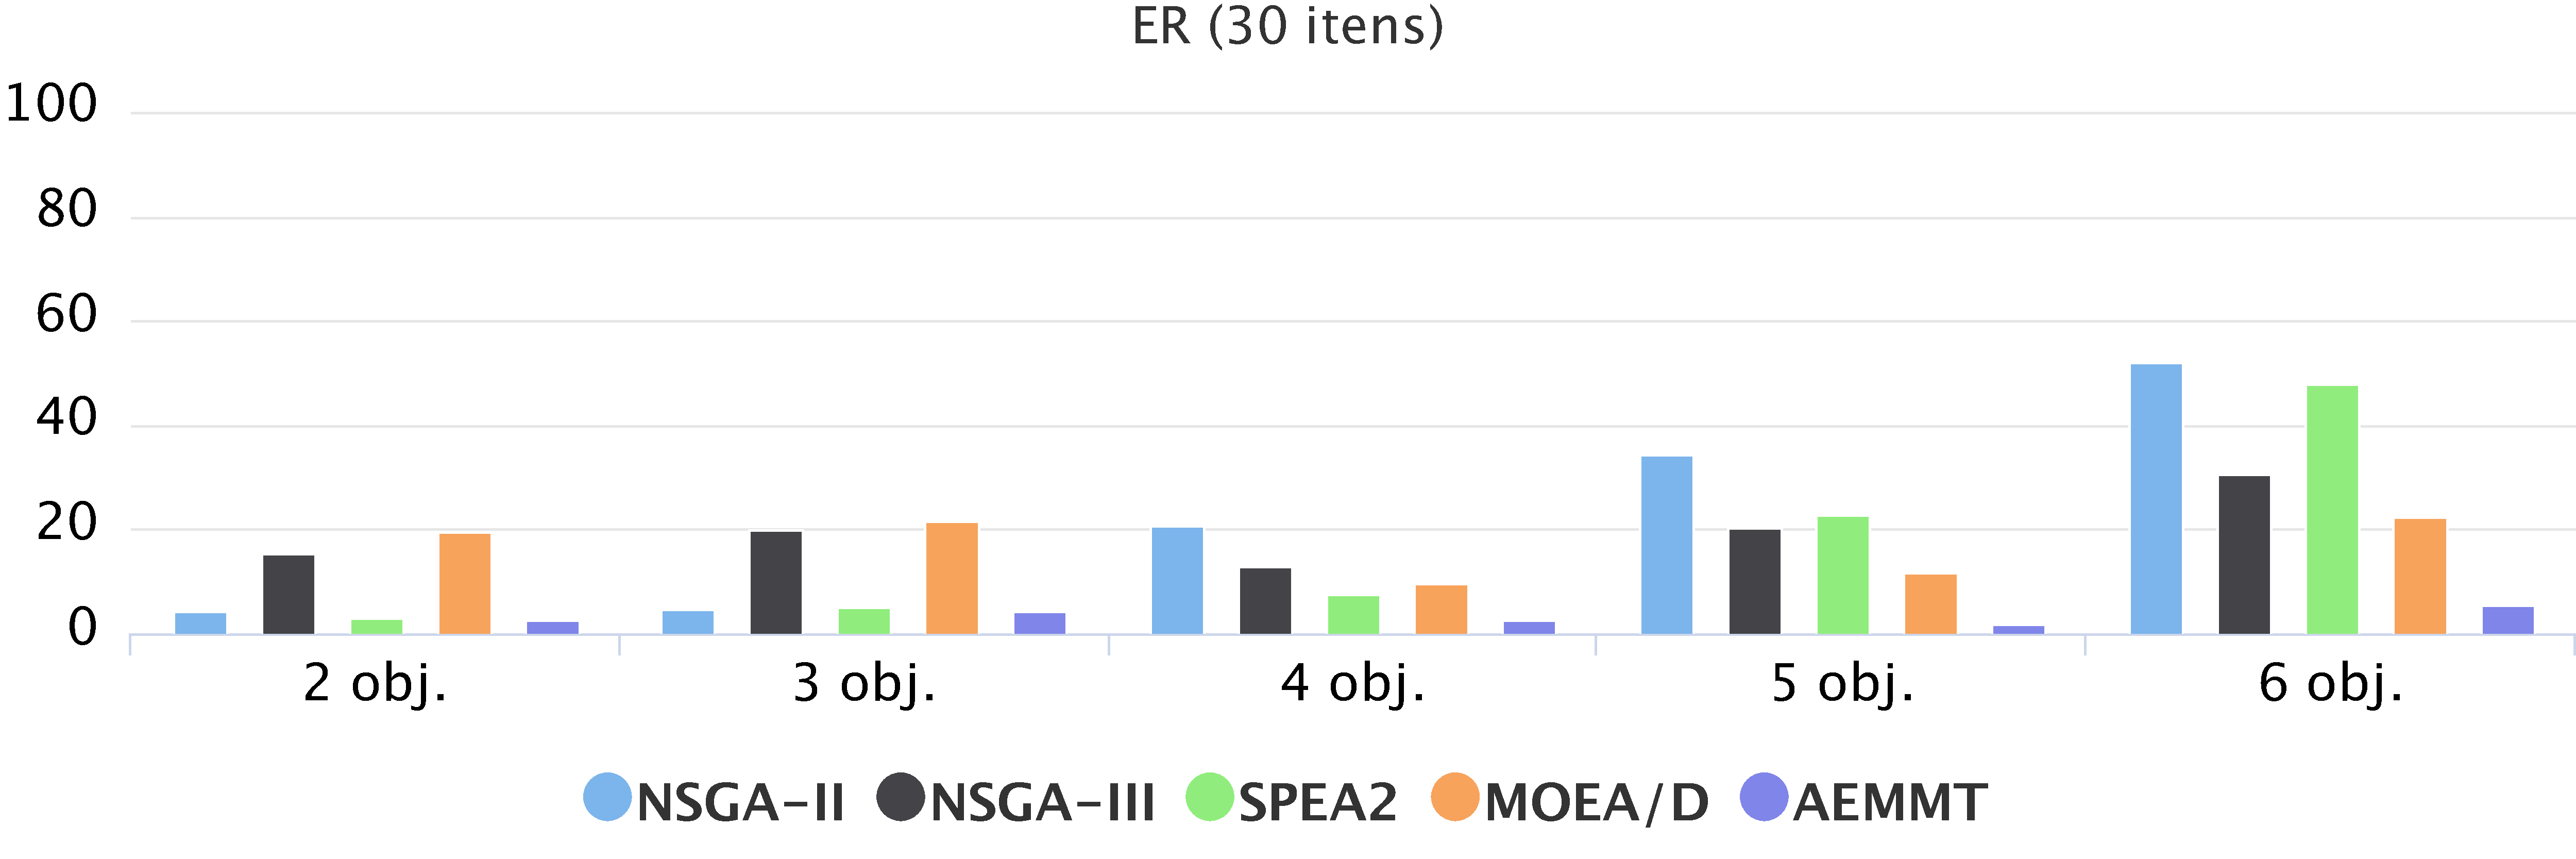
\includegraphics[width=1\textwidth]{cap_experimentos/figs/etapa1/er-mkp-30}
	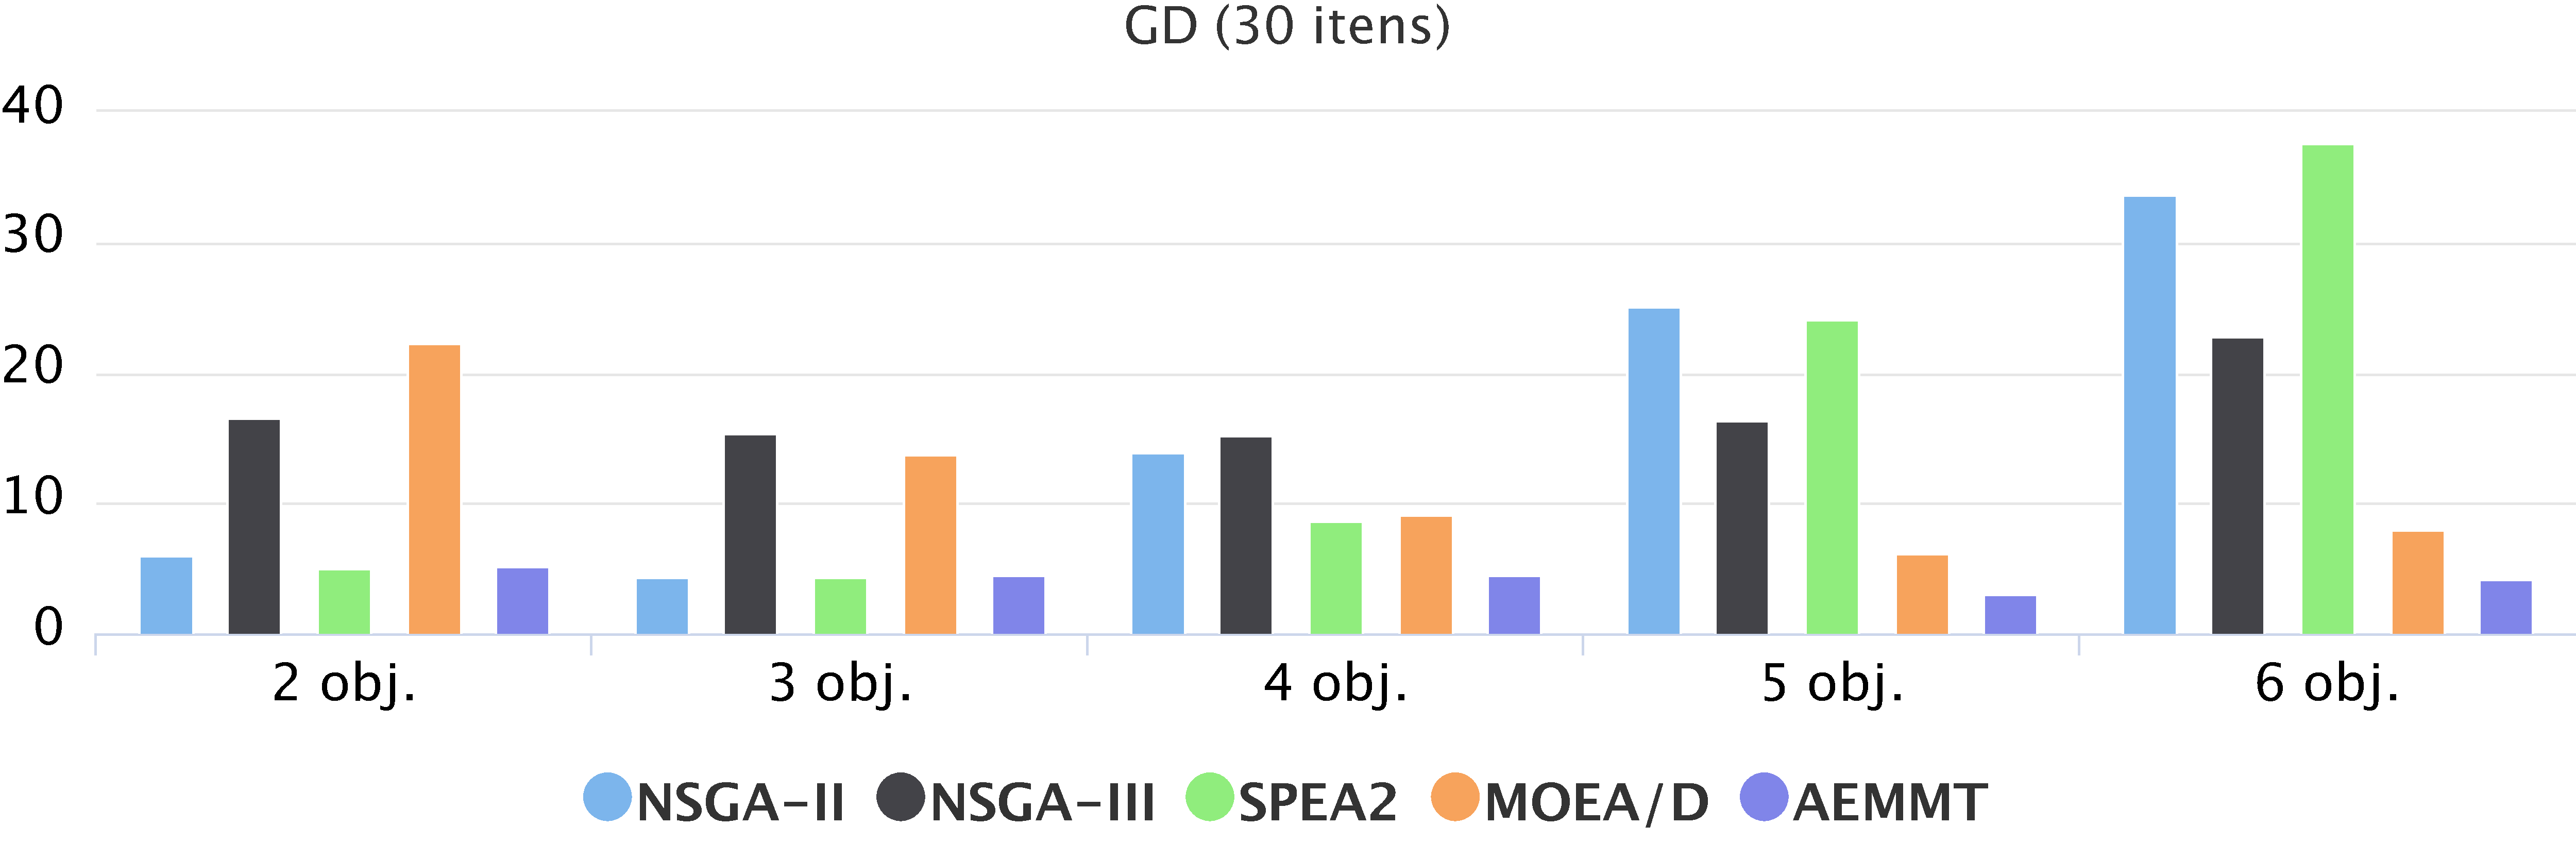
\includegraphics[width=1\textwidth]{cap_experimentos/figs/etapa1/gd-mkp-30}
	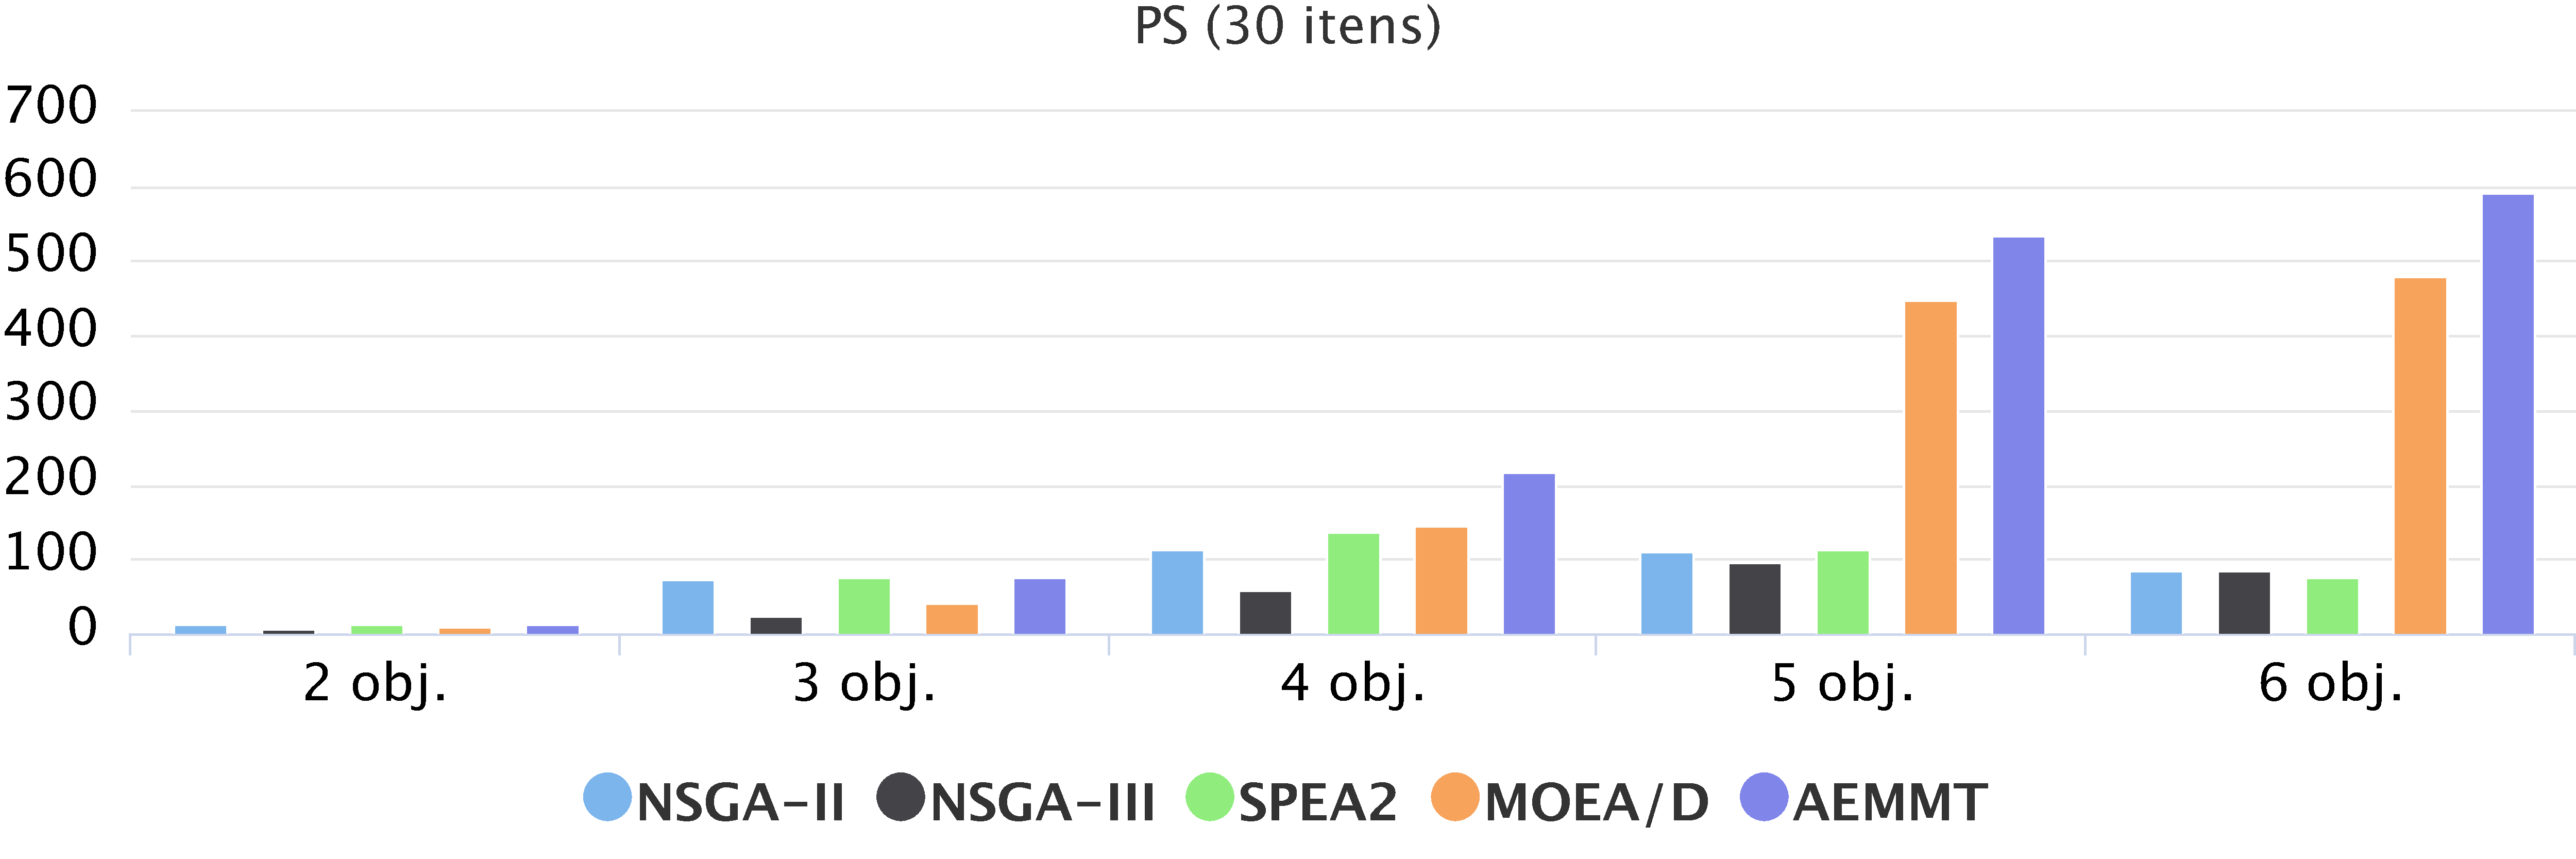
\includegraphics[width=1\textwidth]{cap_experimentos/figs/etapa1/ps-mkp-30}
\end{figure*}

Análise do MKP-30

\begin{figure*}[!htbp]
	\caption{Etapa 1: resultados para o PMM com 50 itens}
	\label{fig_exp1_mkp_50}
	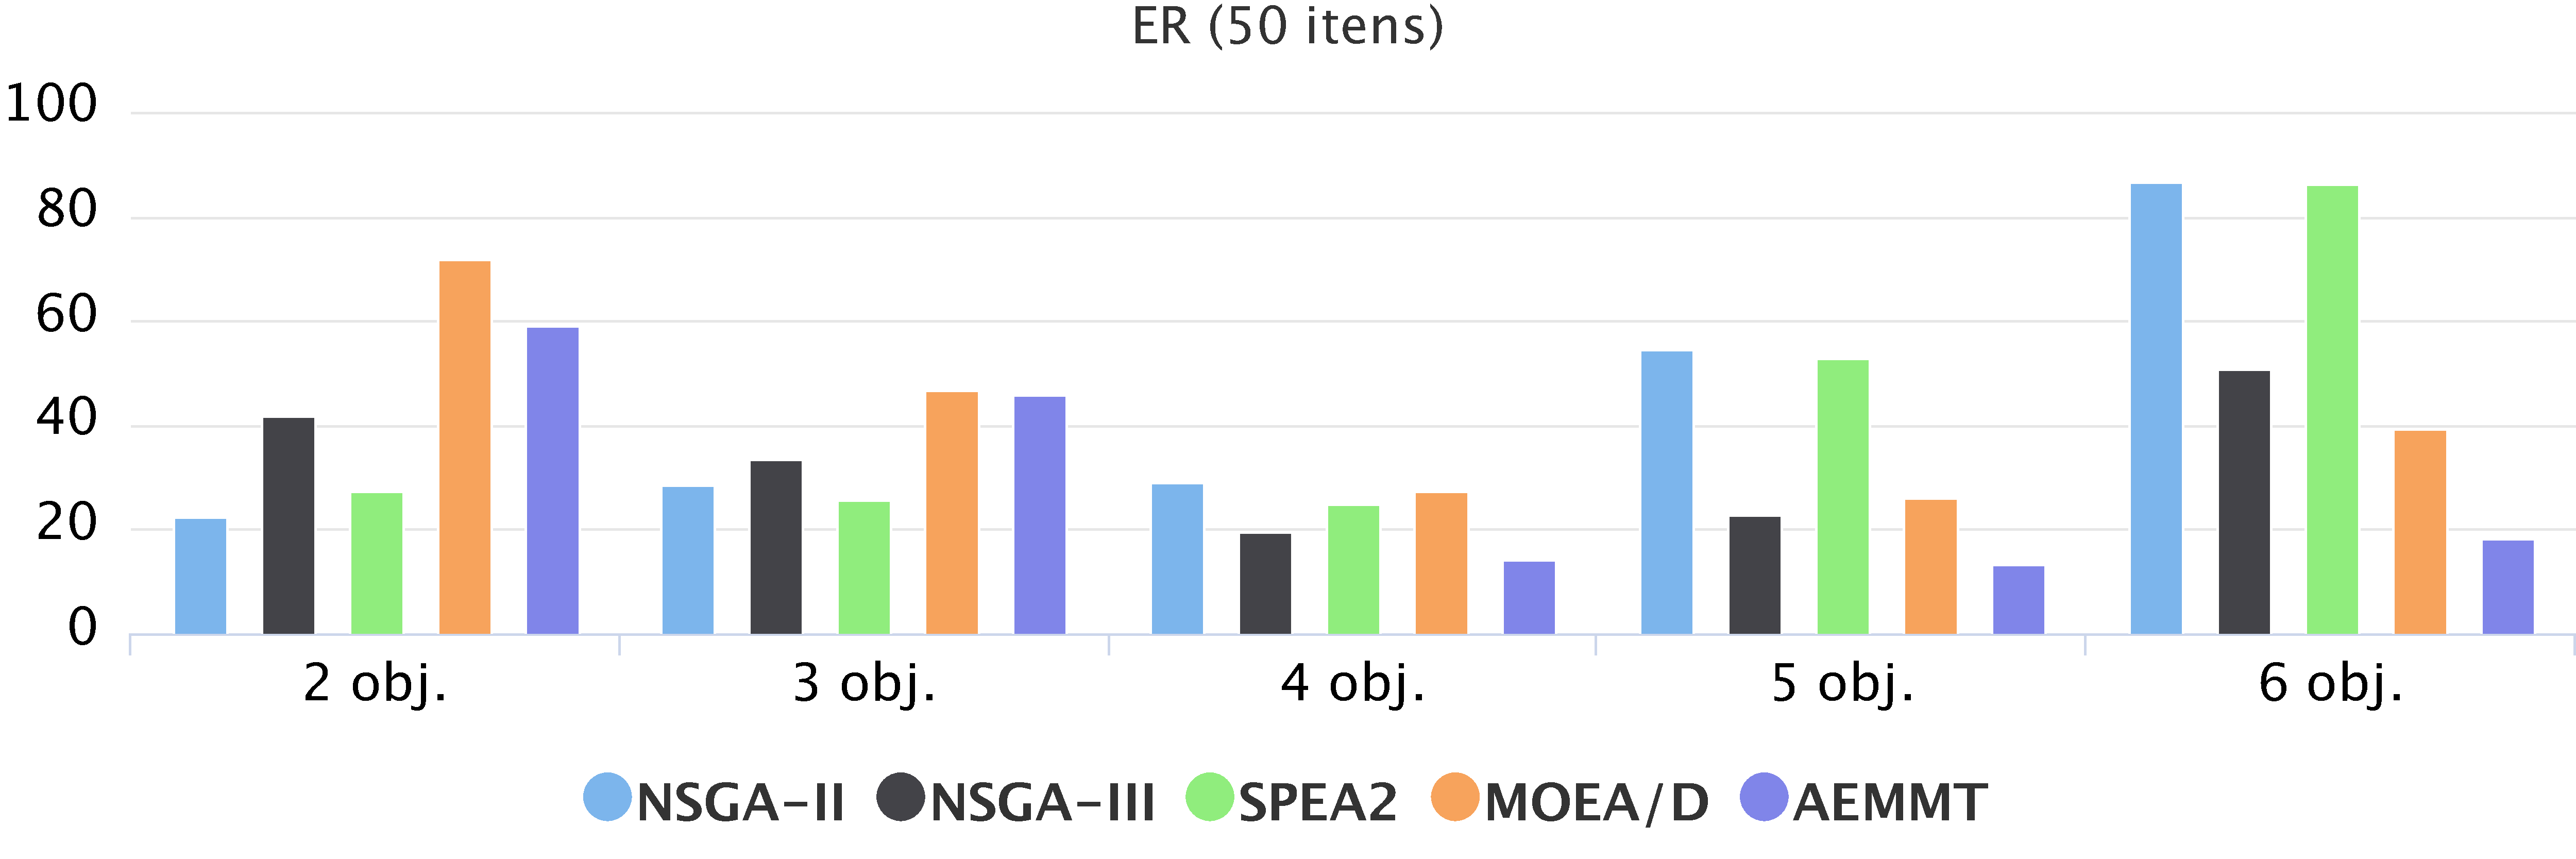
\includegraphics[width=1\textwidth]{cap_experimentos/figs/etapa1/er-mkp-50}
	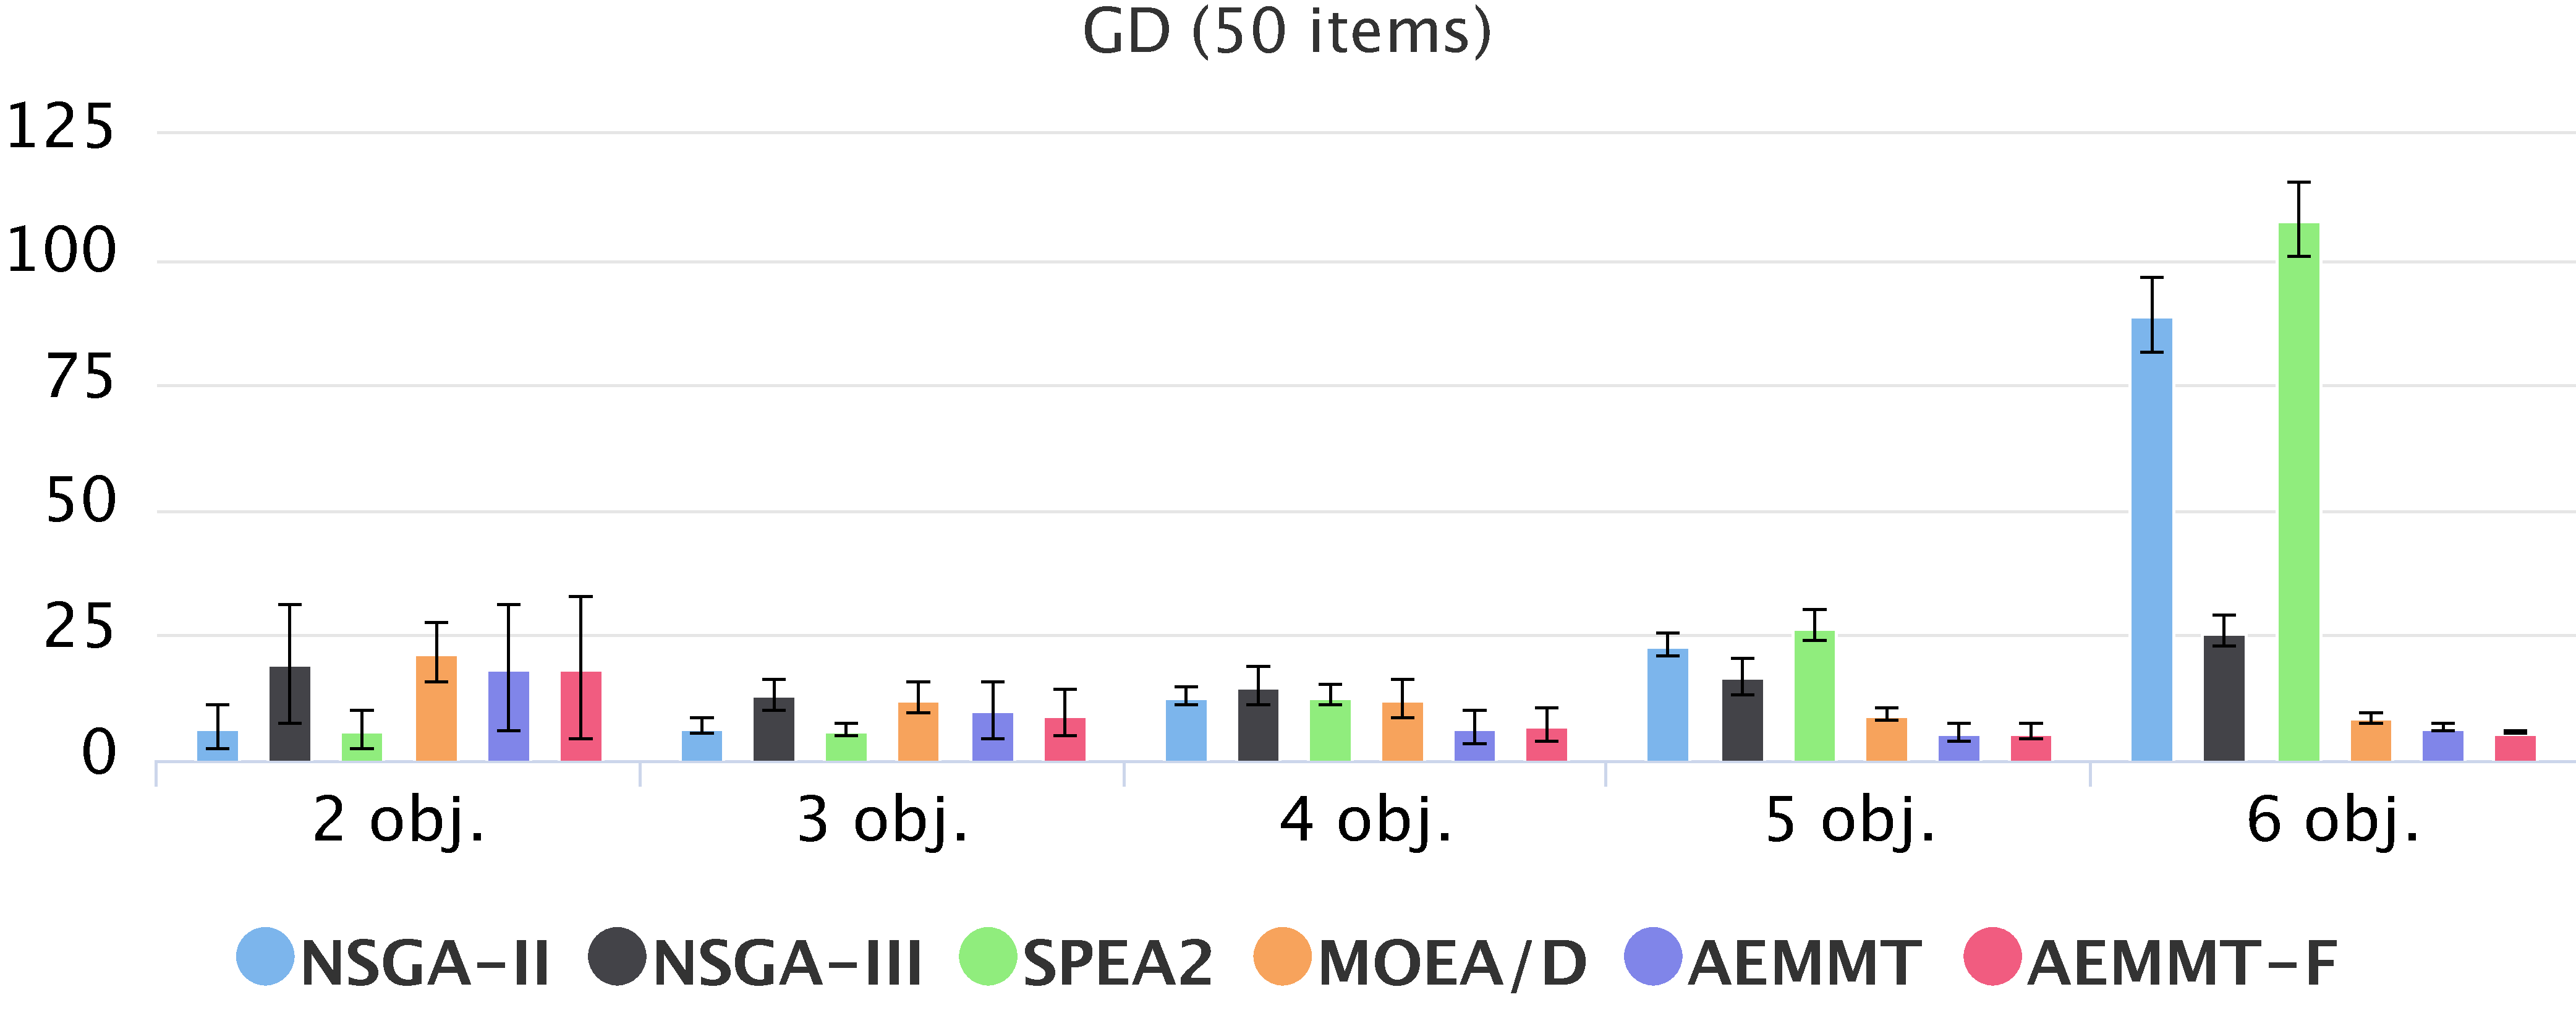
\includegraphics[width=1\textwidth]{cap_experimentos/figs/etapa1/gd-mkp-50}
	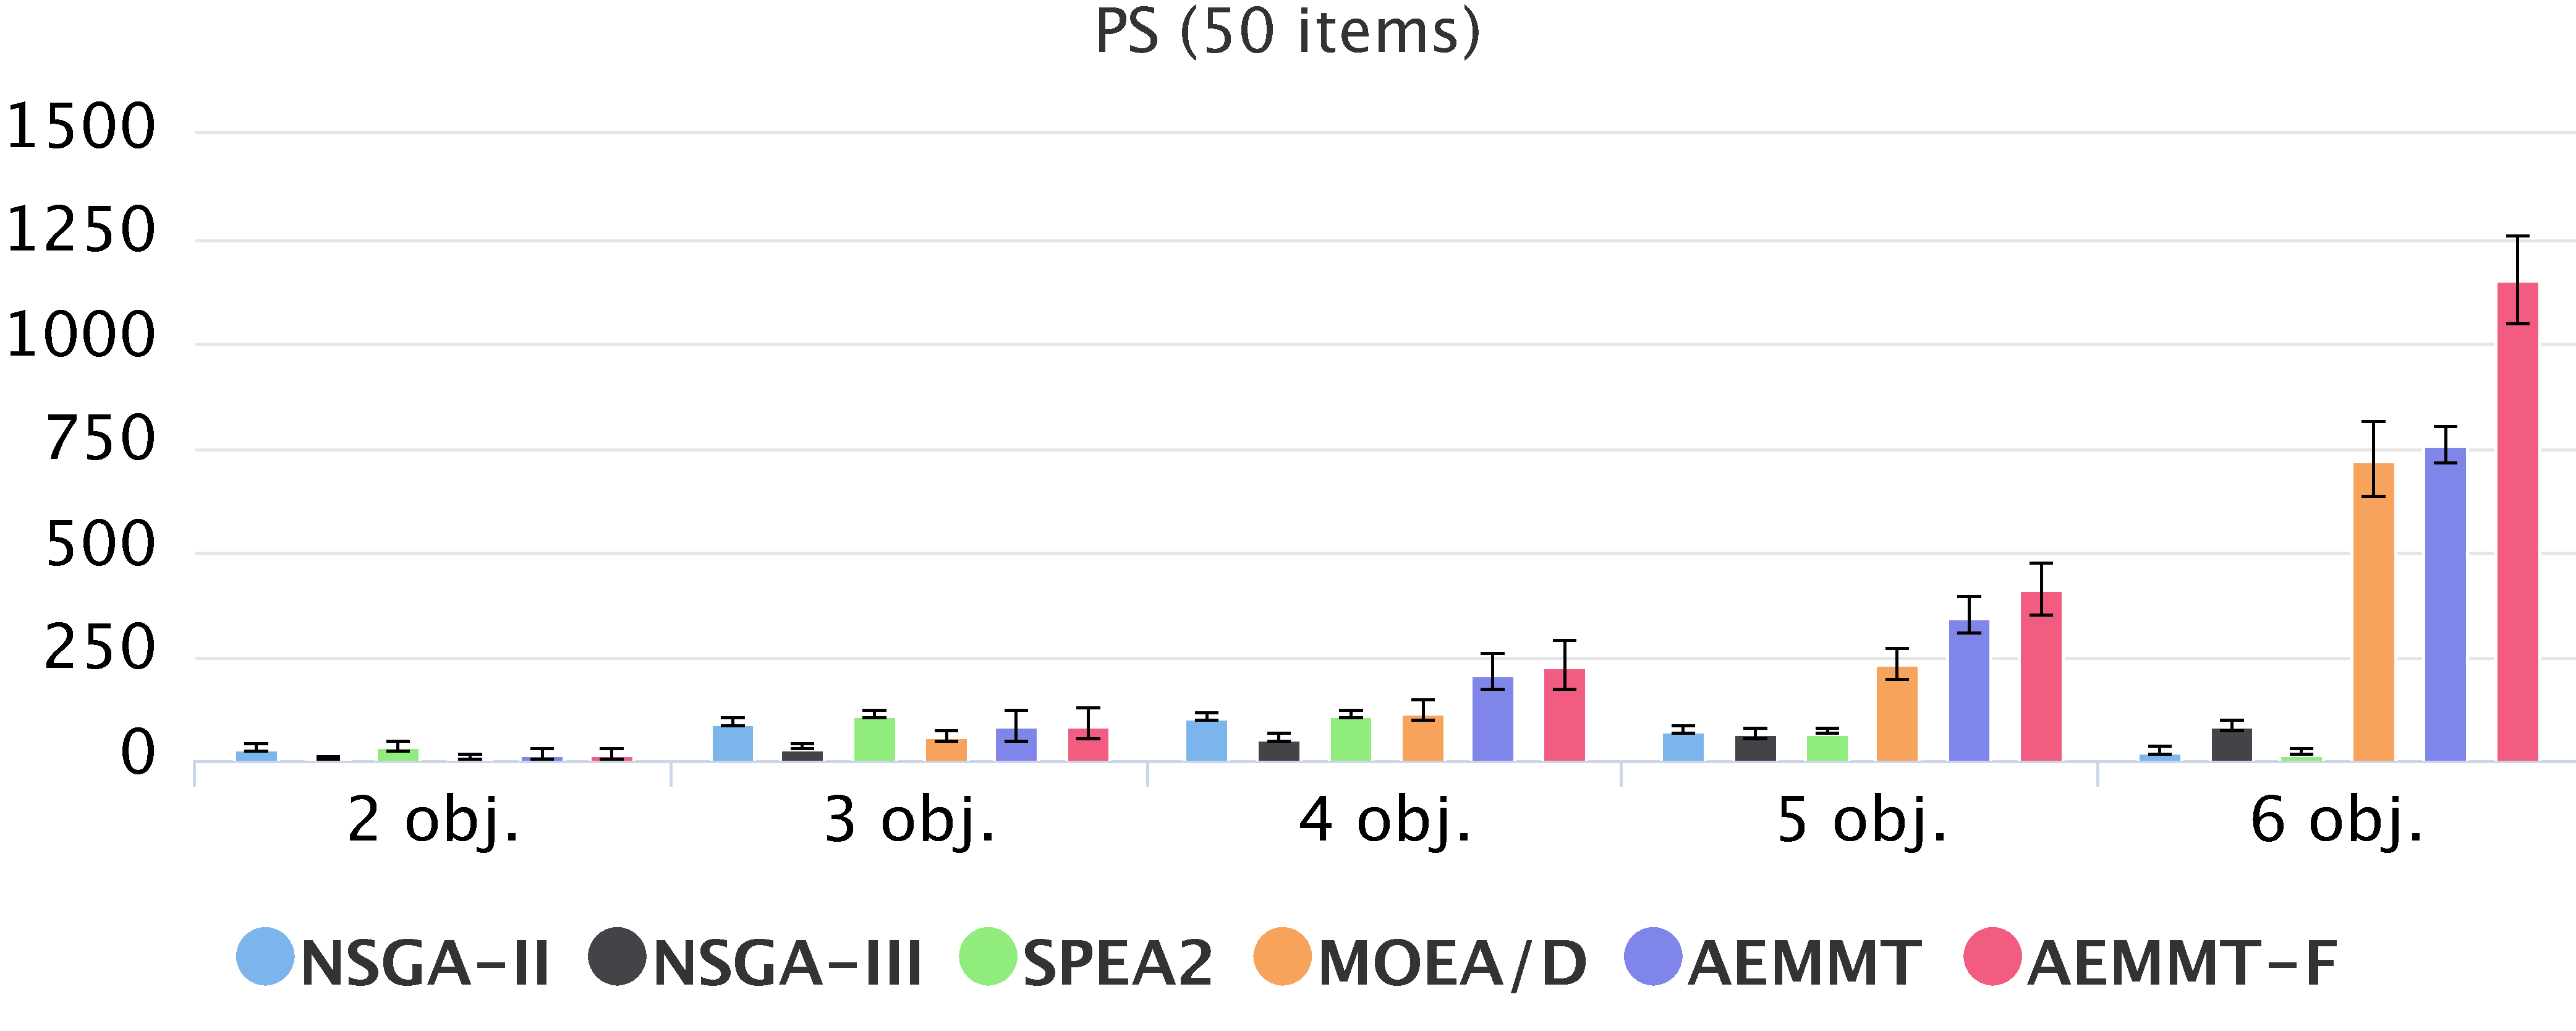
\includegraphics[width=1\textwidth]{cap_experimentos/figs/etapa1/ps-mkp-50}
\end{figure*}

Análise do MKP-50

\begin{figure*}[!htbp]
	\caption{Etapa 1: resultados para o PMM com 100 itens}
	\label{fig_exp1_mkp_100}
	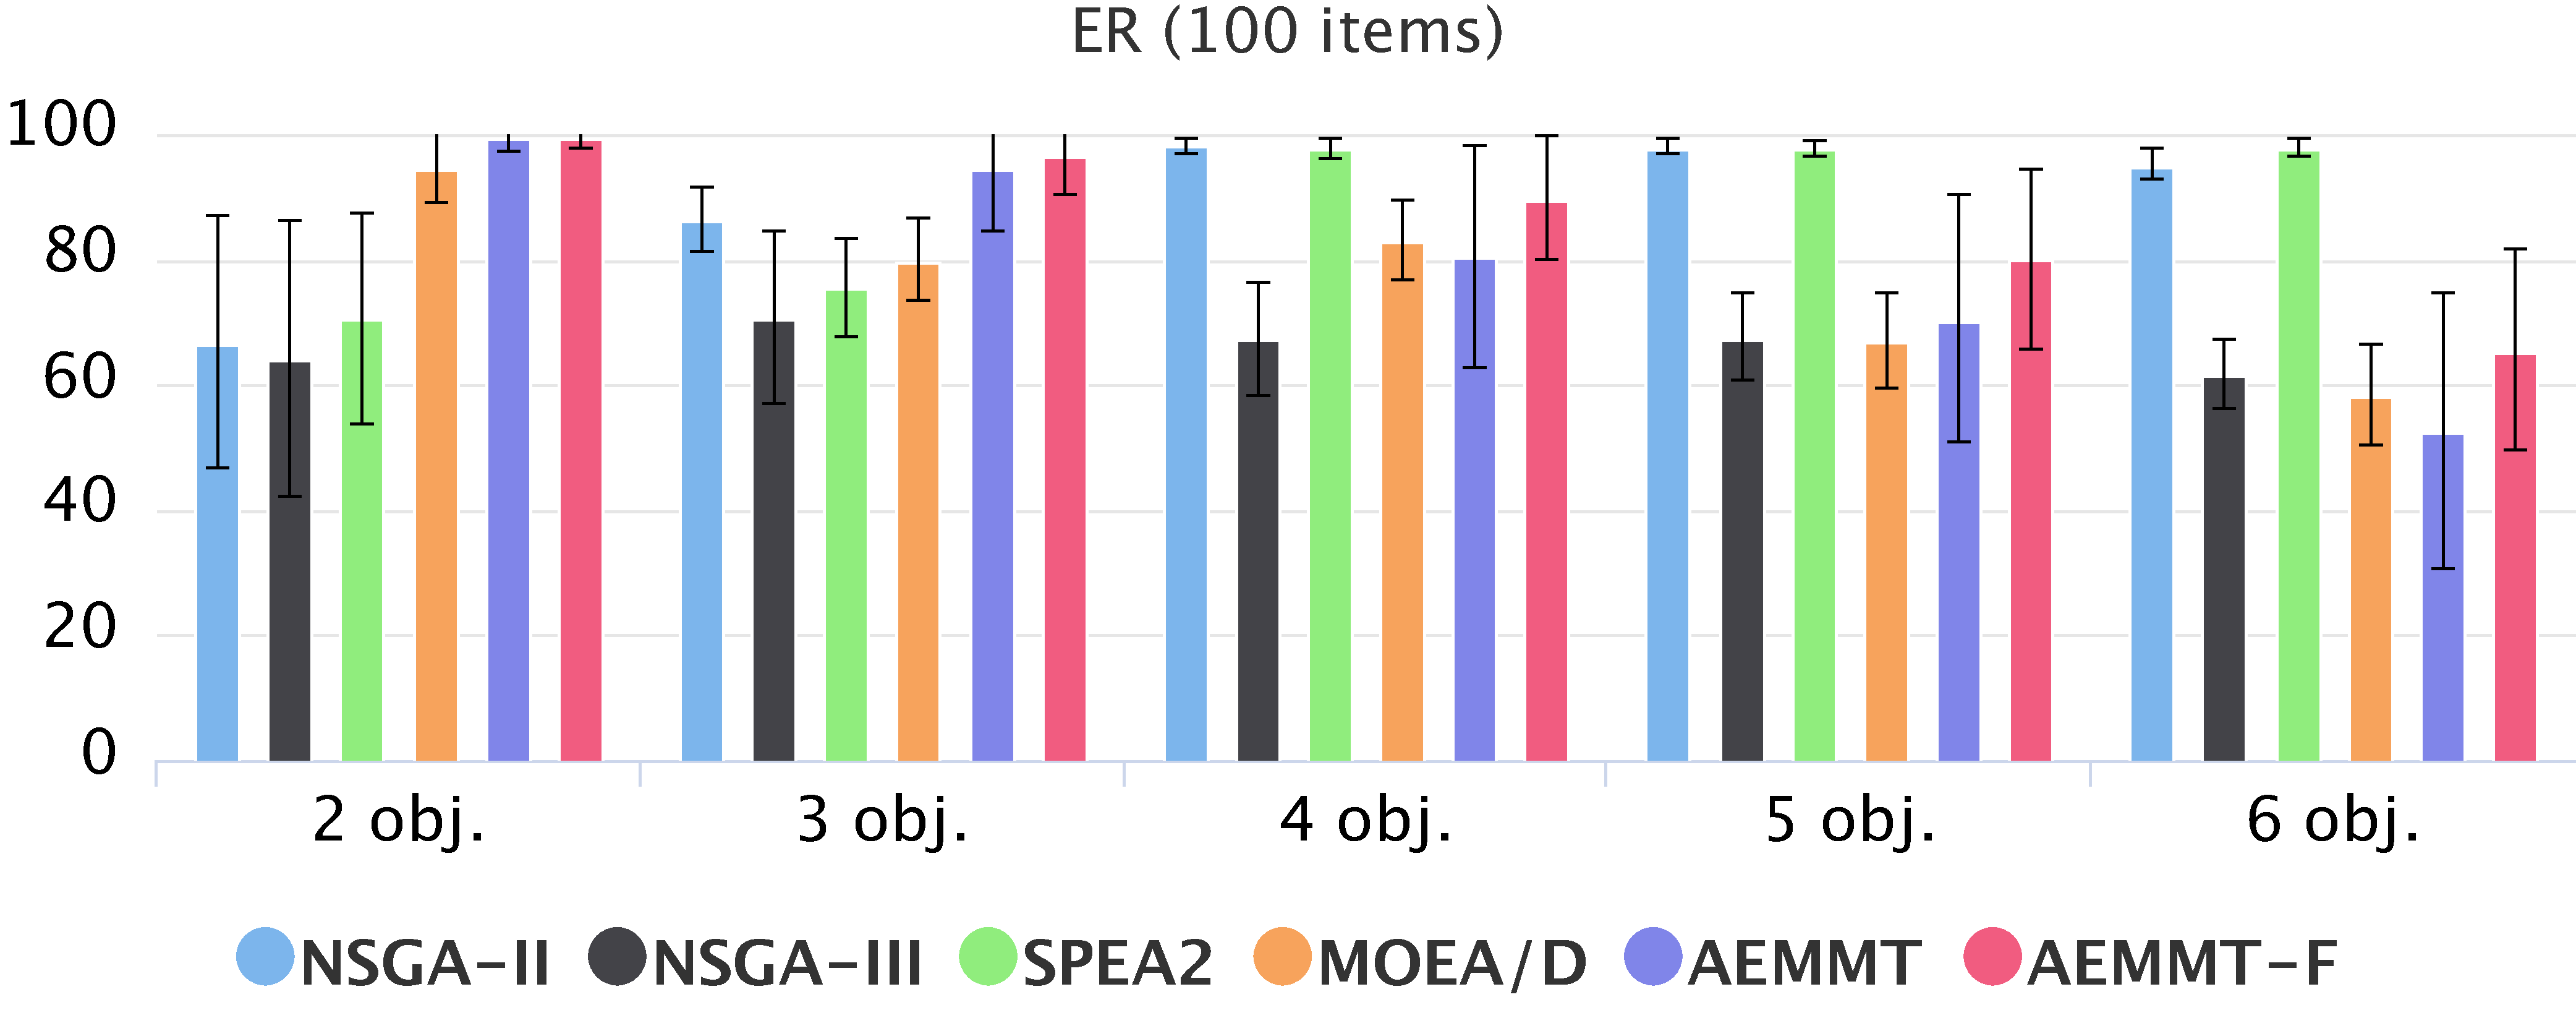
\includegraphics[width=1\textwidth]{cap_experimentos/figs/etapa1/er-mkp-100}
	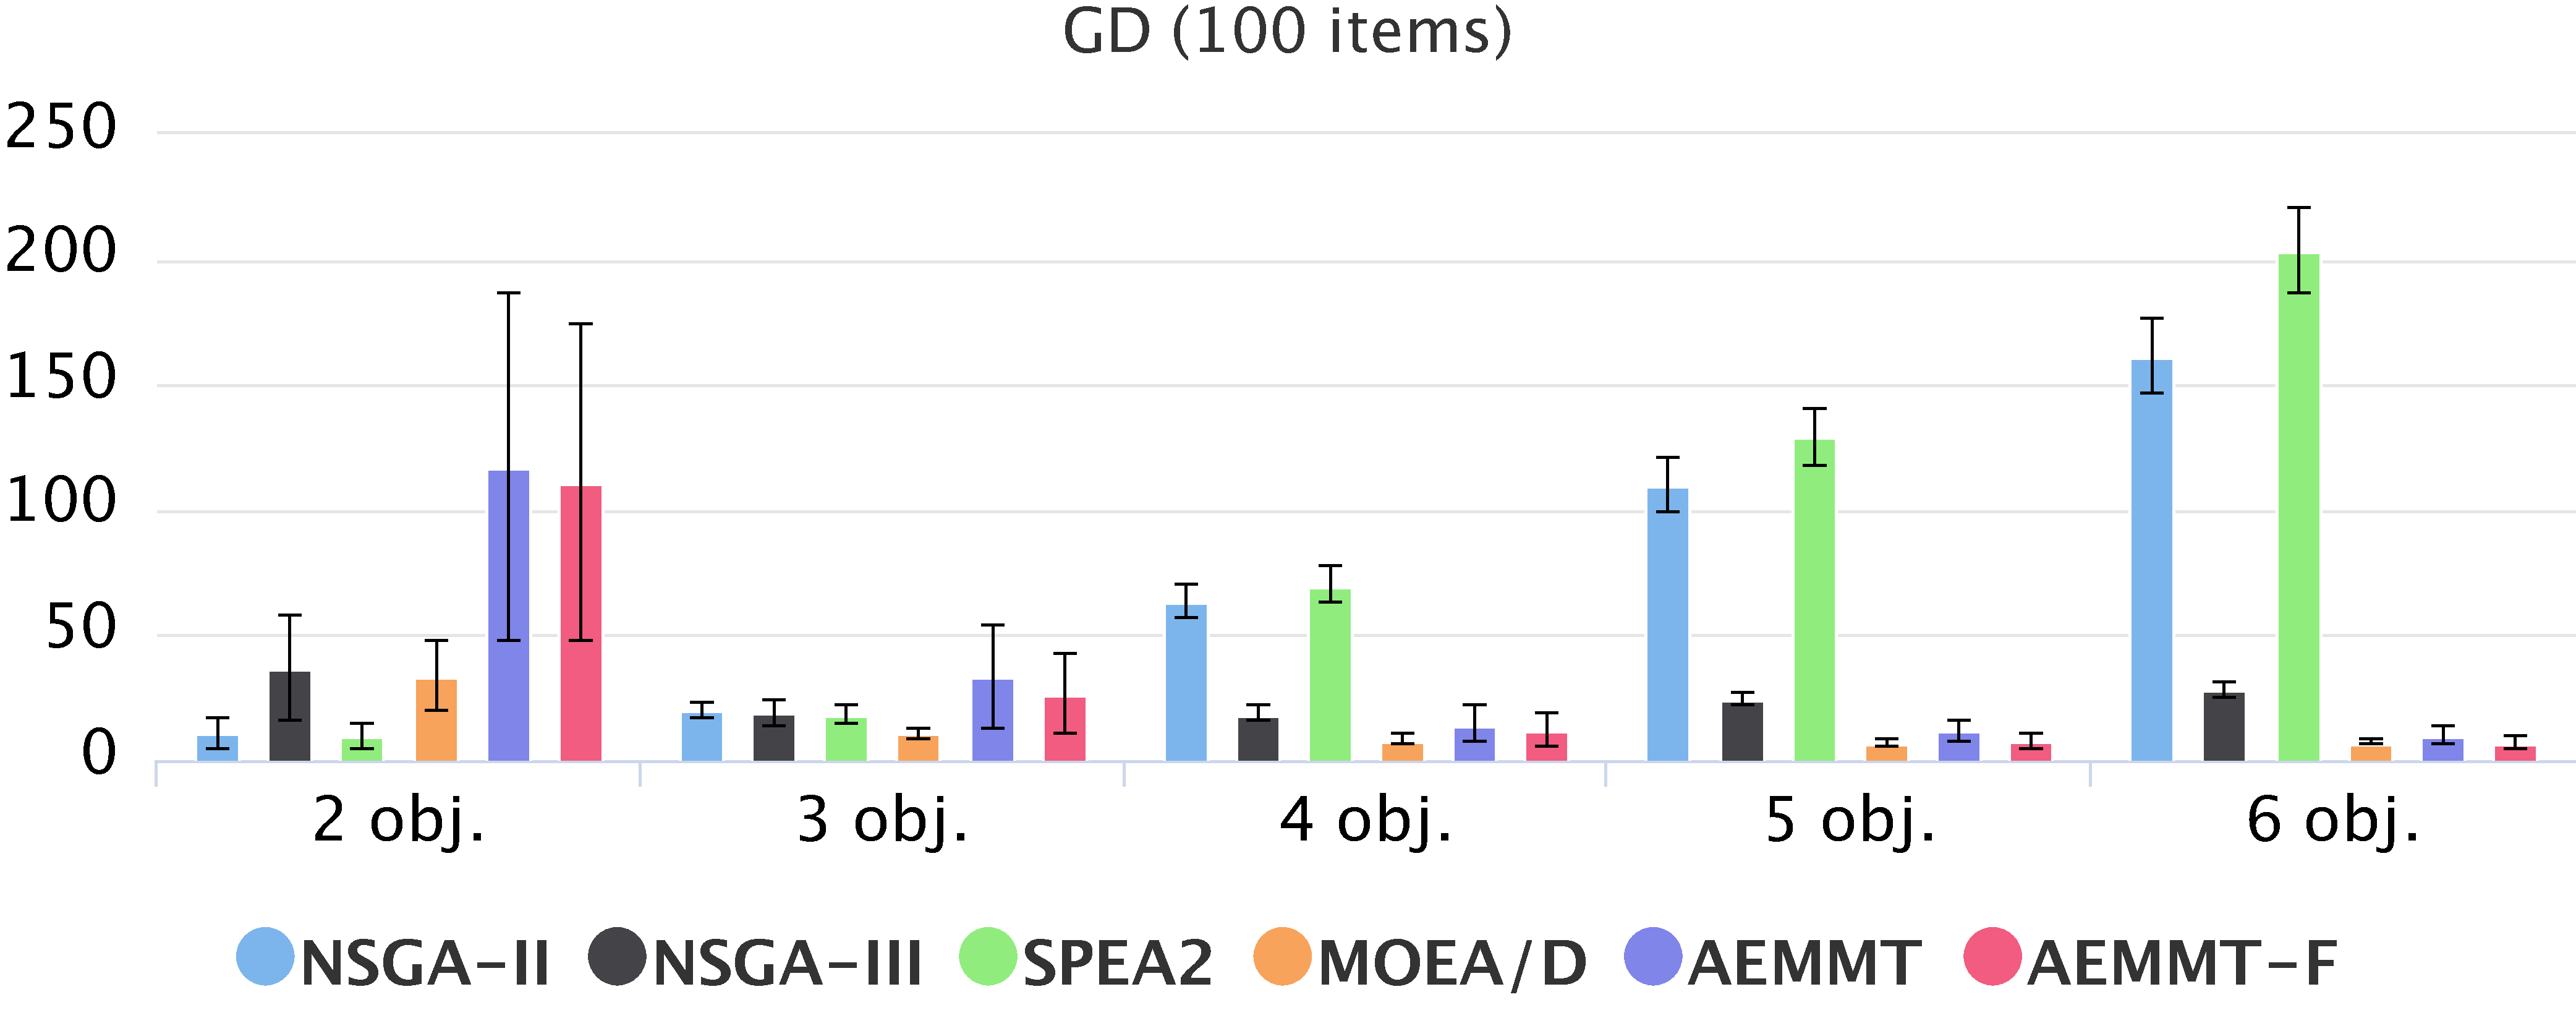
\includegraphics[width=1\textwidth]{cap_experimentos/figs/etapa1/gd-mkp-100}
	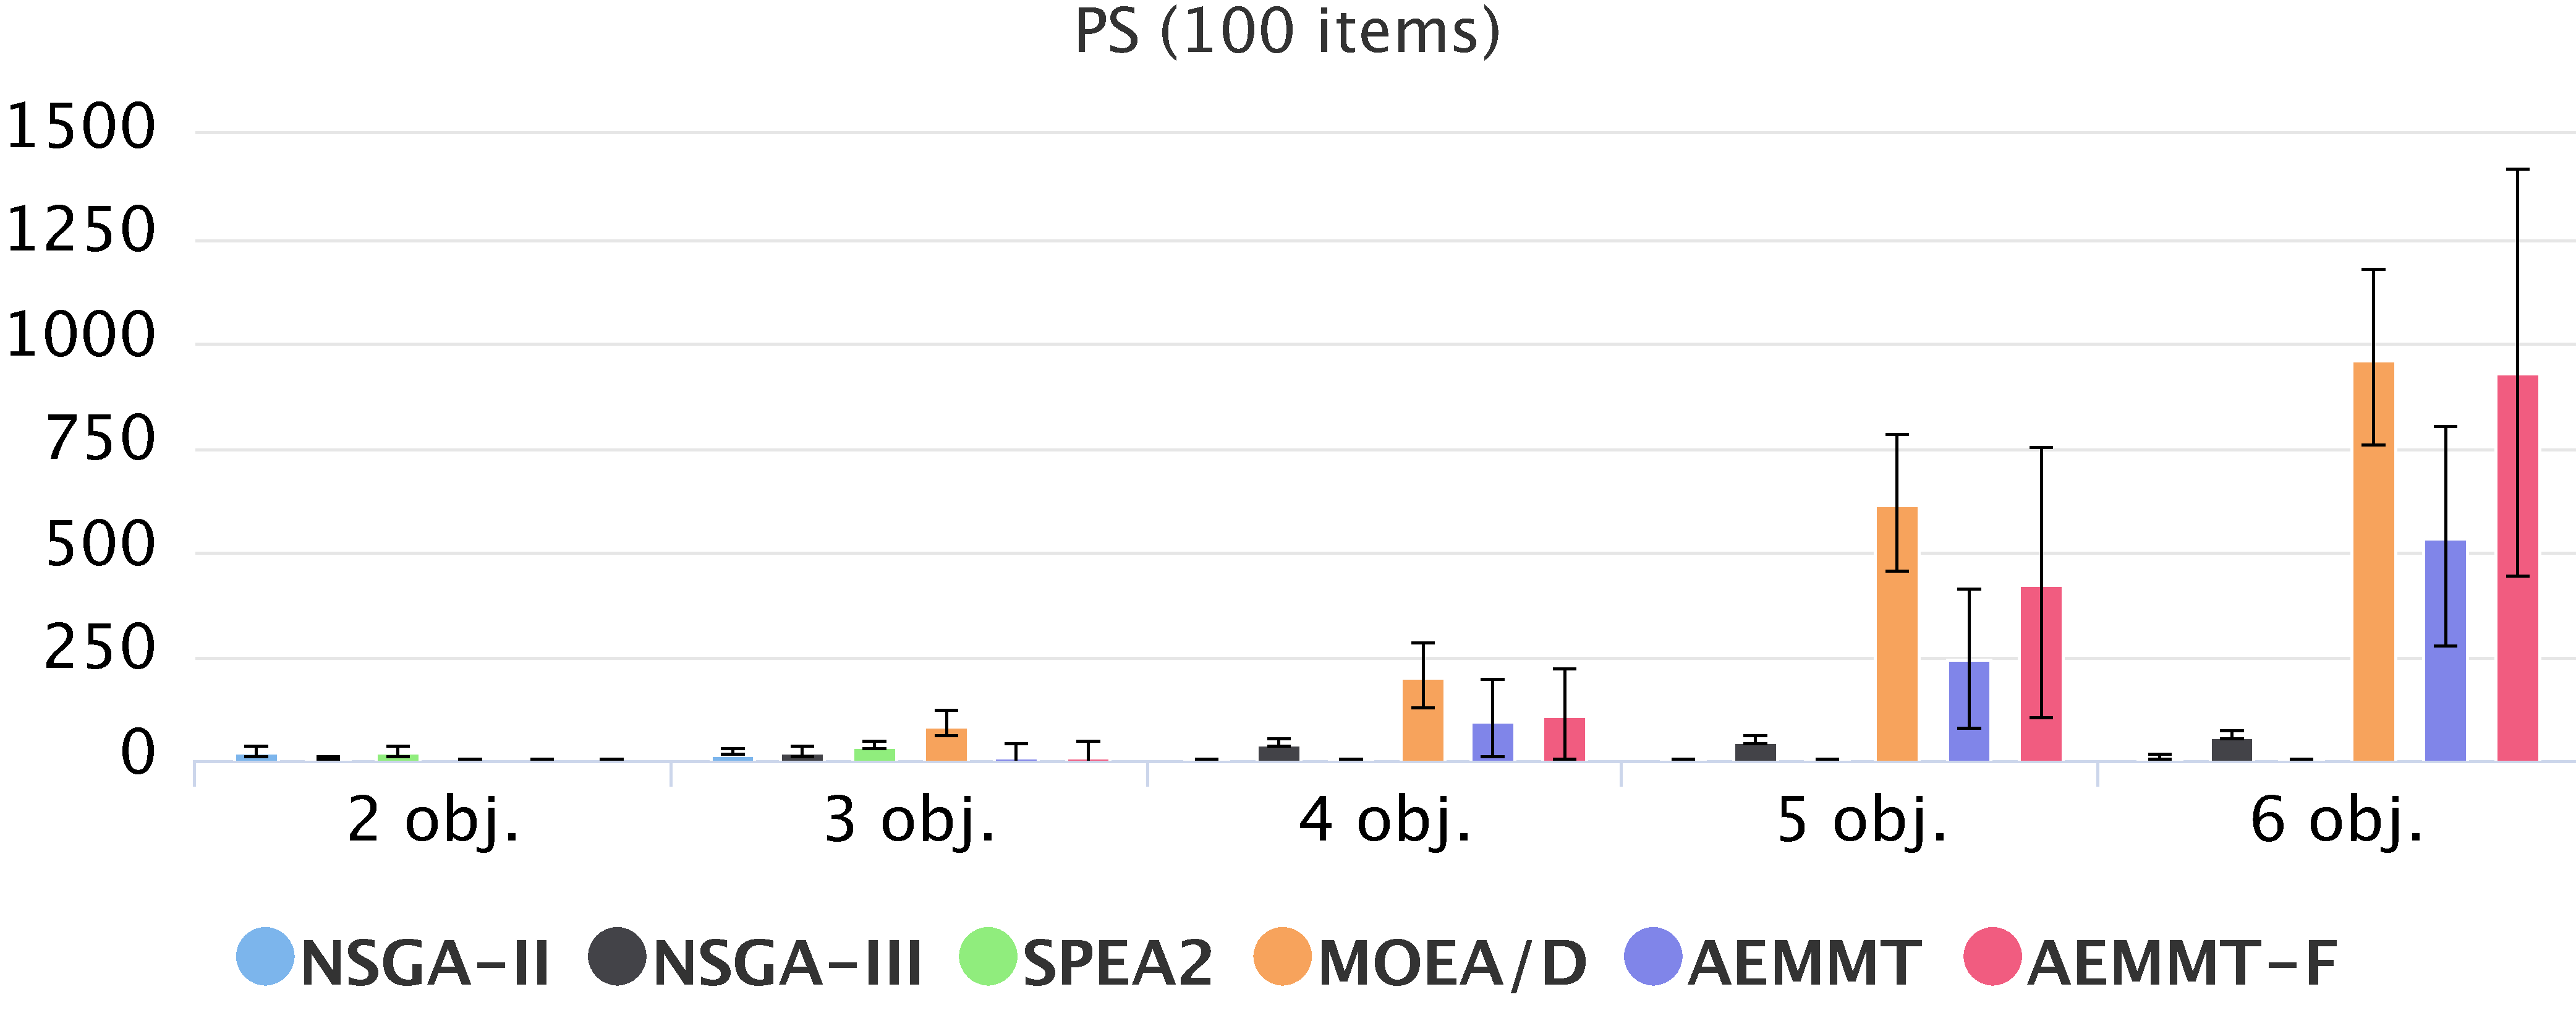
\includegraphics[width=1\textwidth]{cap_experimentos/figs/etapa1/ps-mkp-100}
\end{figure*}

Análise do MKP-100

\begin{figure*}[!htbp]
	\caption{Etapa 1: resultados agrupados para o PMM com 30, 50 e 100 itens}
	\label{fig_exp1_mkp_todos}
	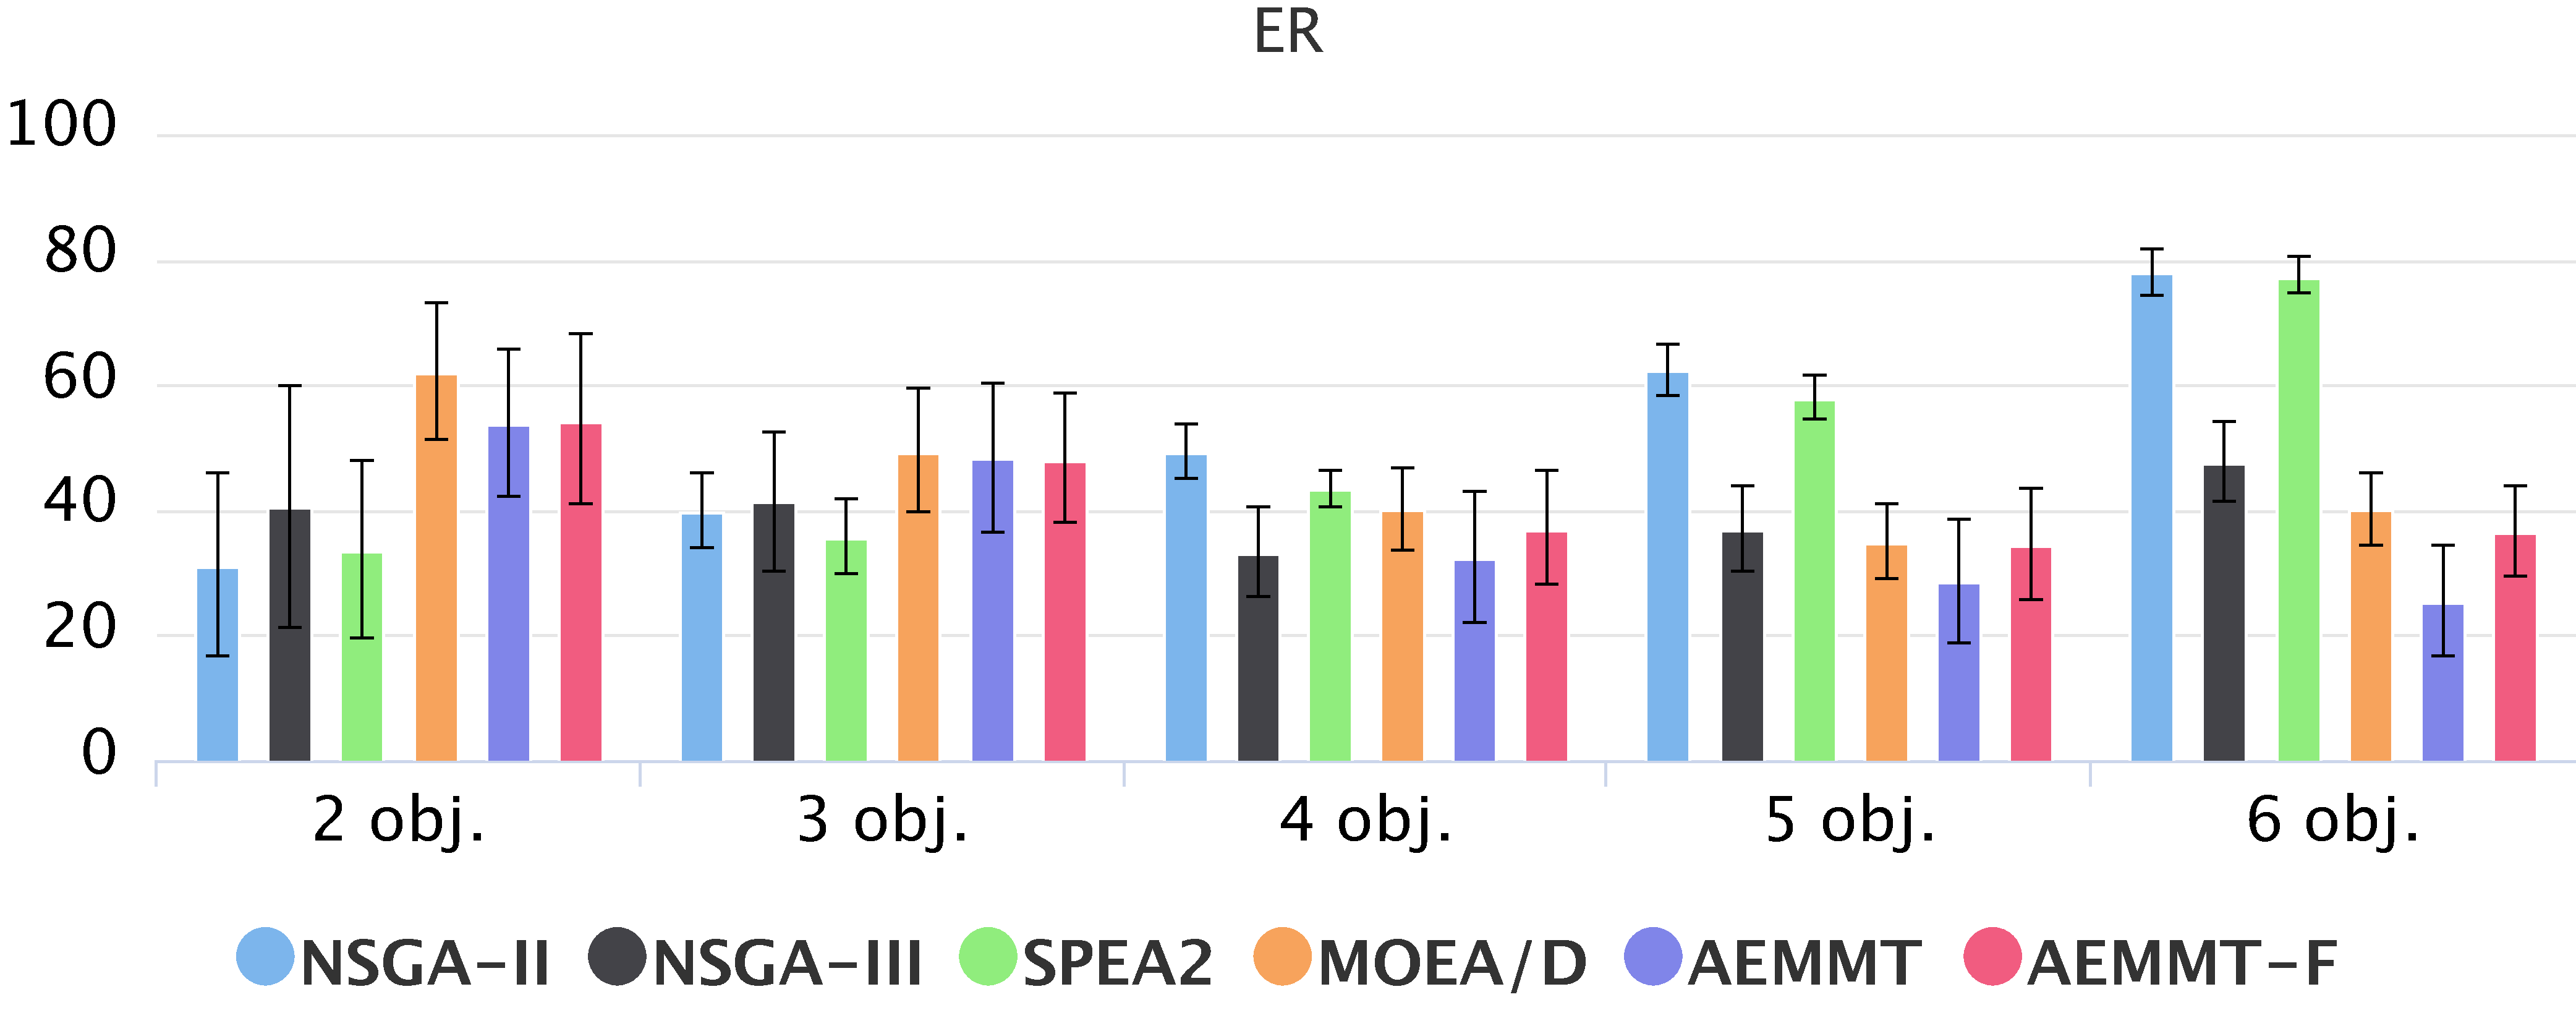
\includegraphics[width=1\textwidth]{cap_experimentos/figs/etapa1/er-mkp-todos}
	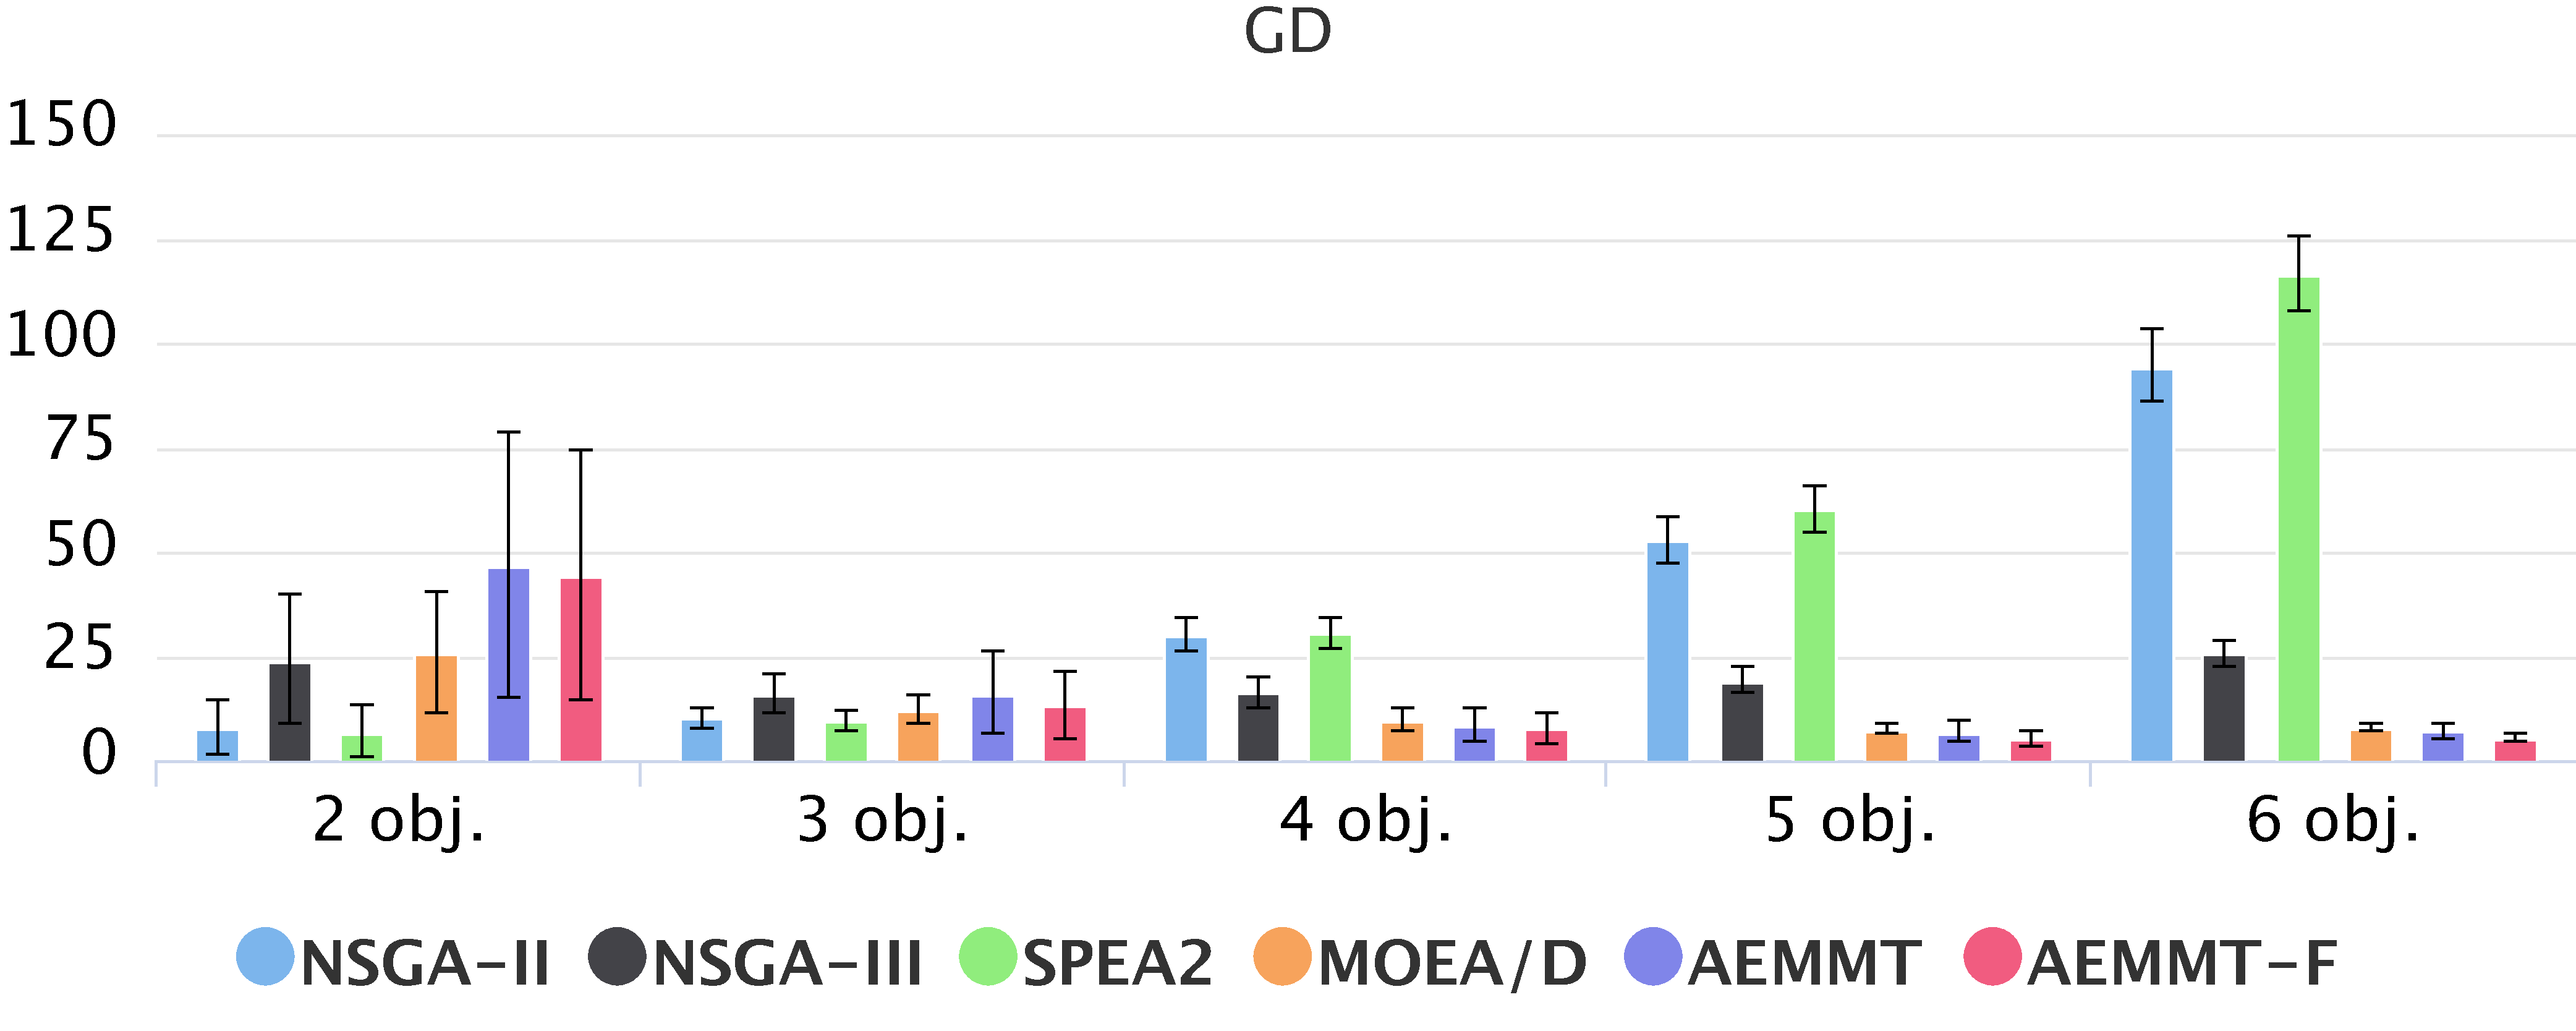
\includegraphics[width=1\textwidth]{cap_experimentos/figs/etapa1/gd-mkp-todos}
	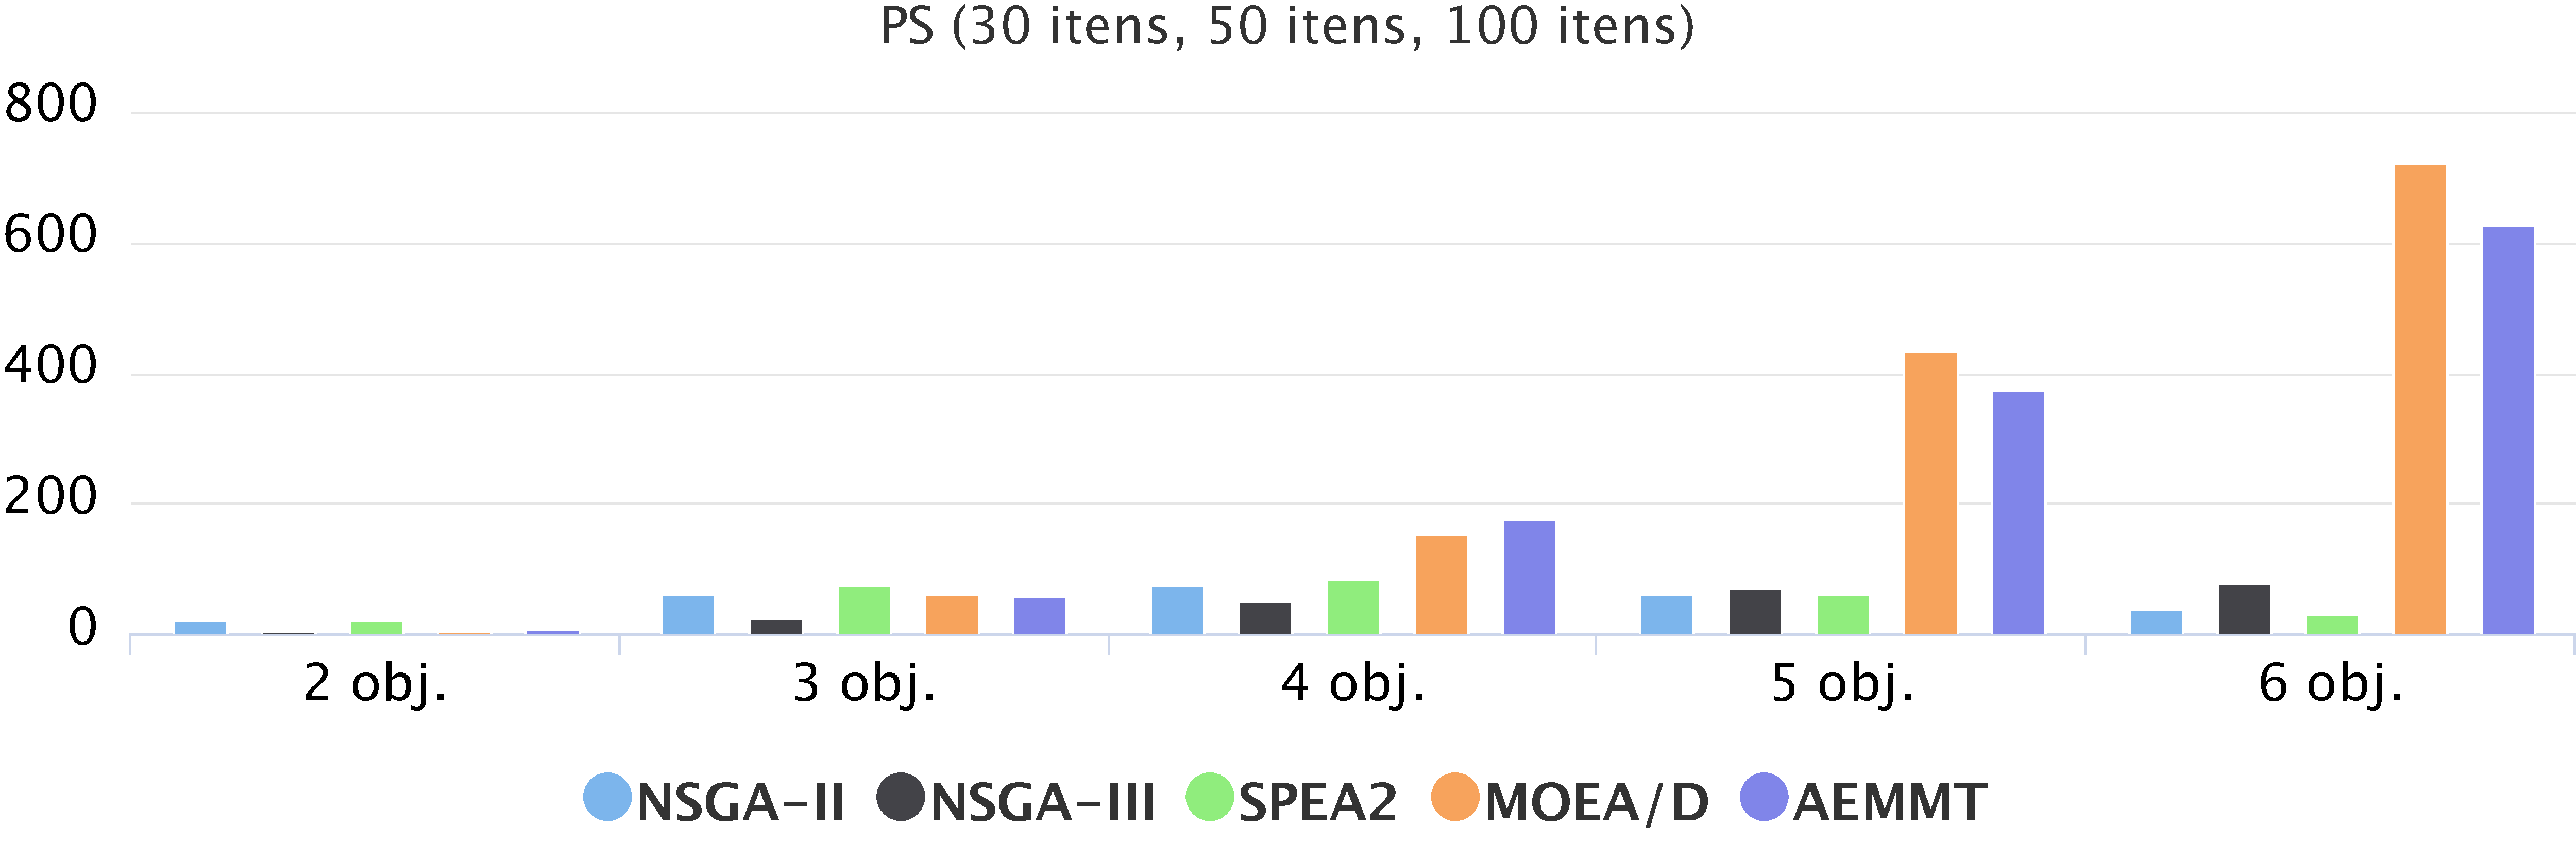
\includegraphics[width=1\textwidth]{cap_experimentos/figs/etapa1/ps-mkp-todos}
\end{figure*}

Análise geral do MKP

\begin{figure*}[!htbp]
	\caption{Etapa 1: resultados para o PRM na rede $R_1$}
	\label{fig_exp1_mrp_r1}
	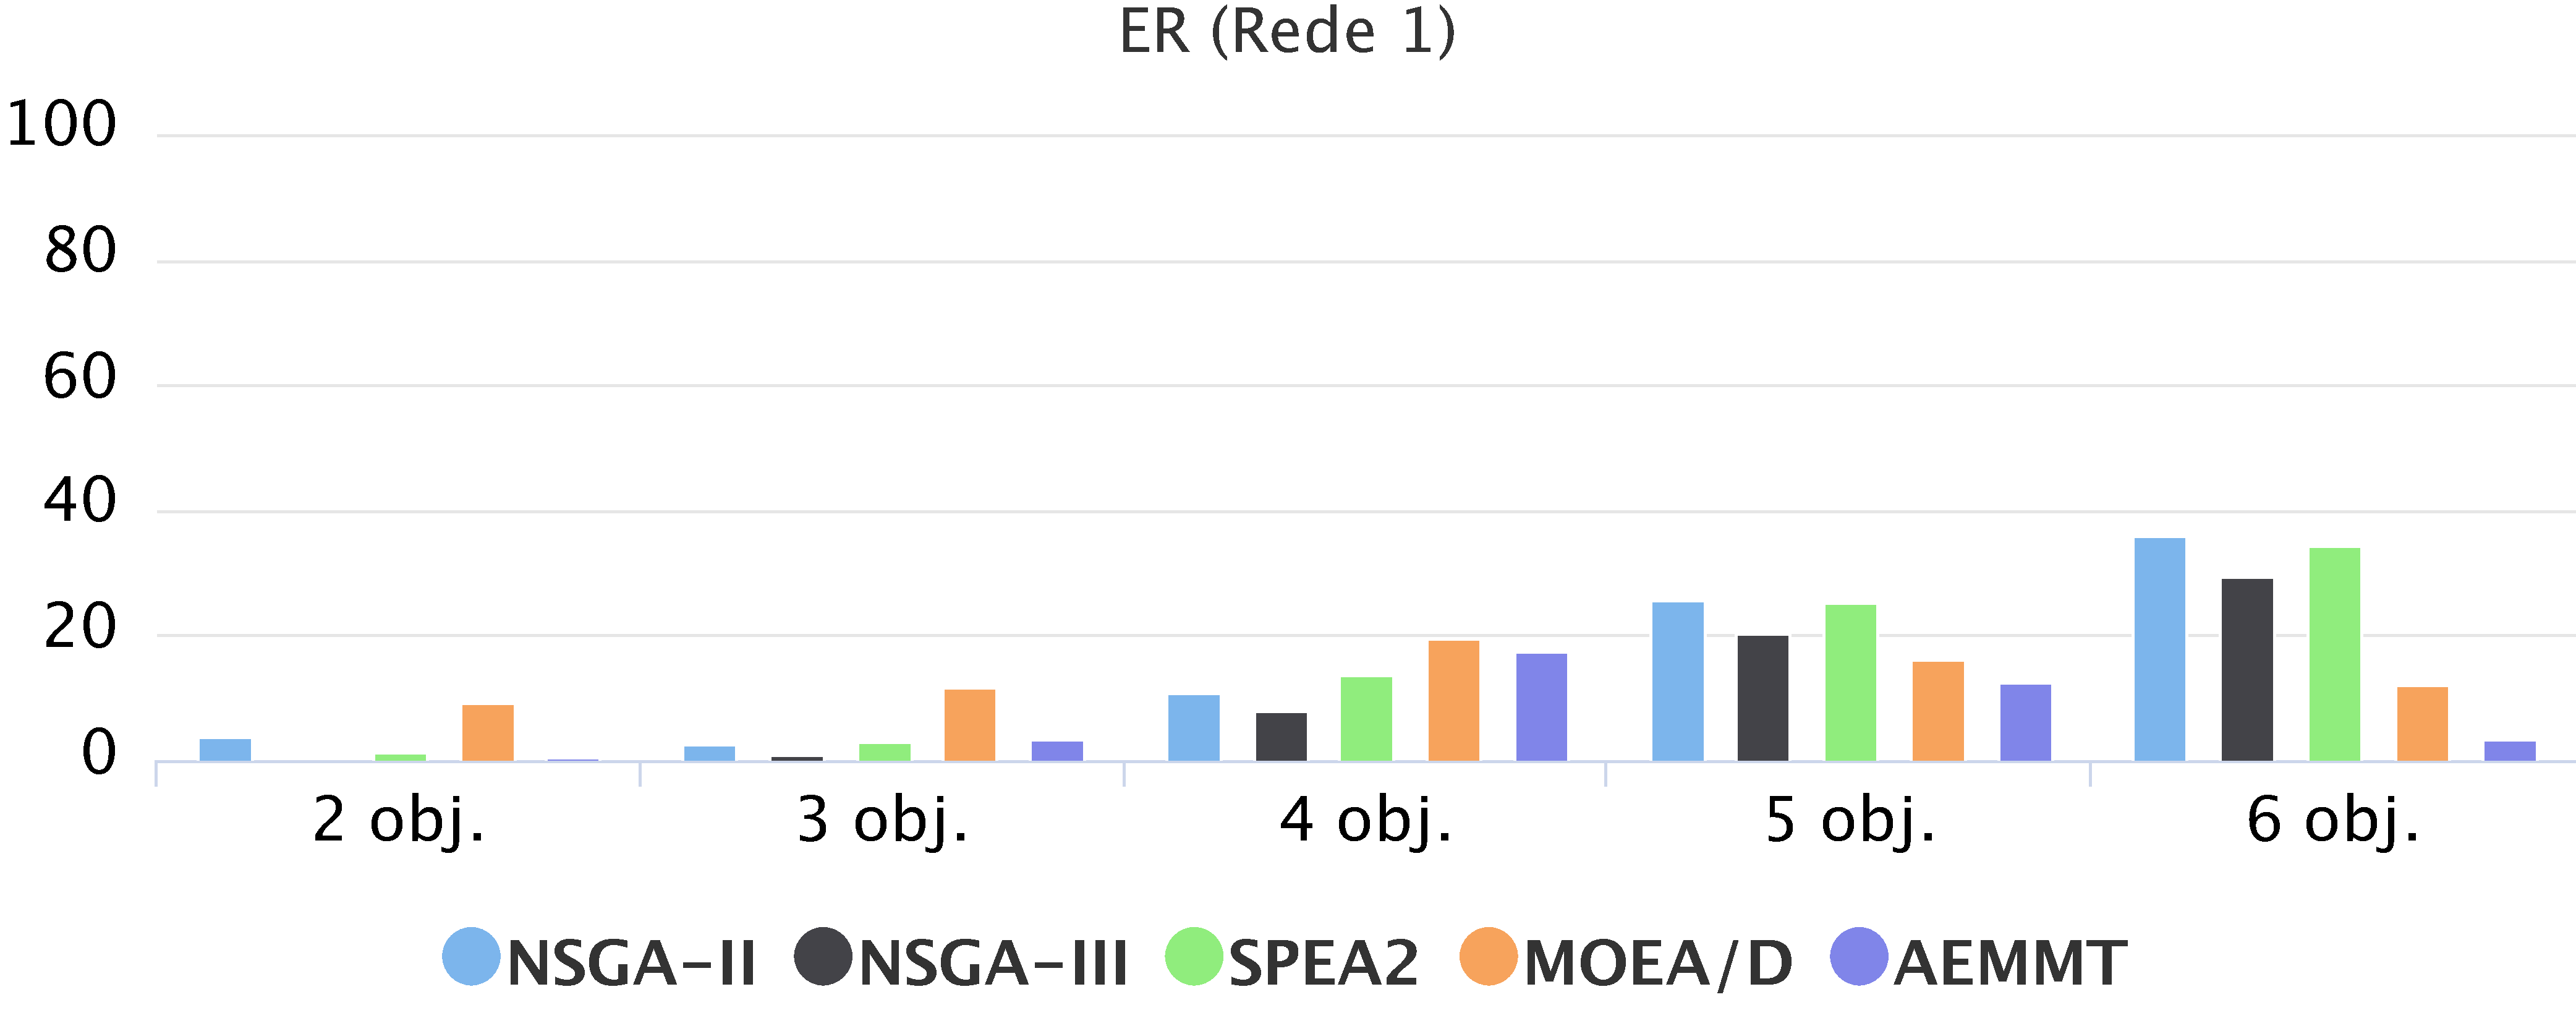
\includegraphics[width=1\textwidth]{cap_experimentos/figs/etapa1/er-mrp-r1}
	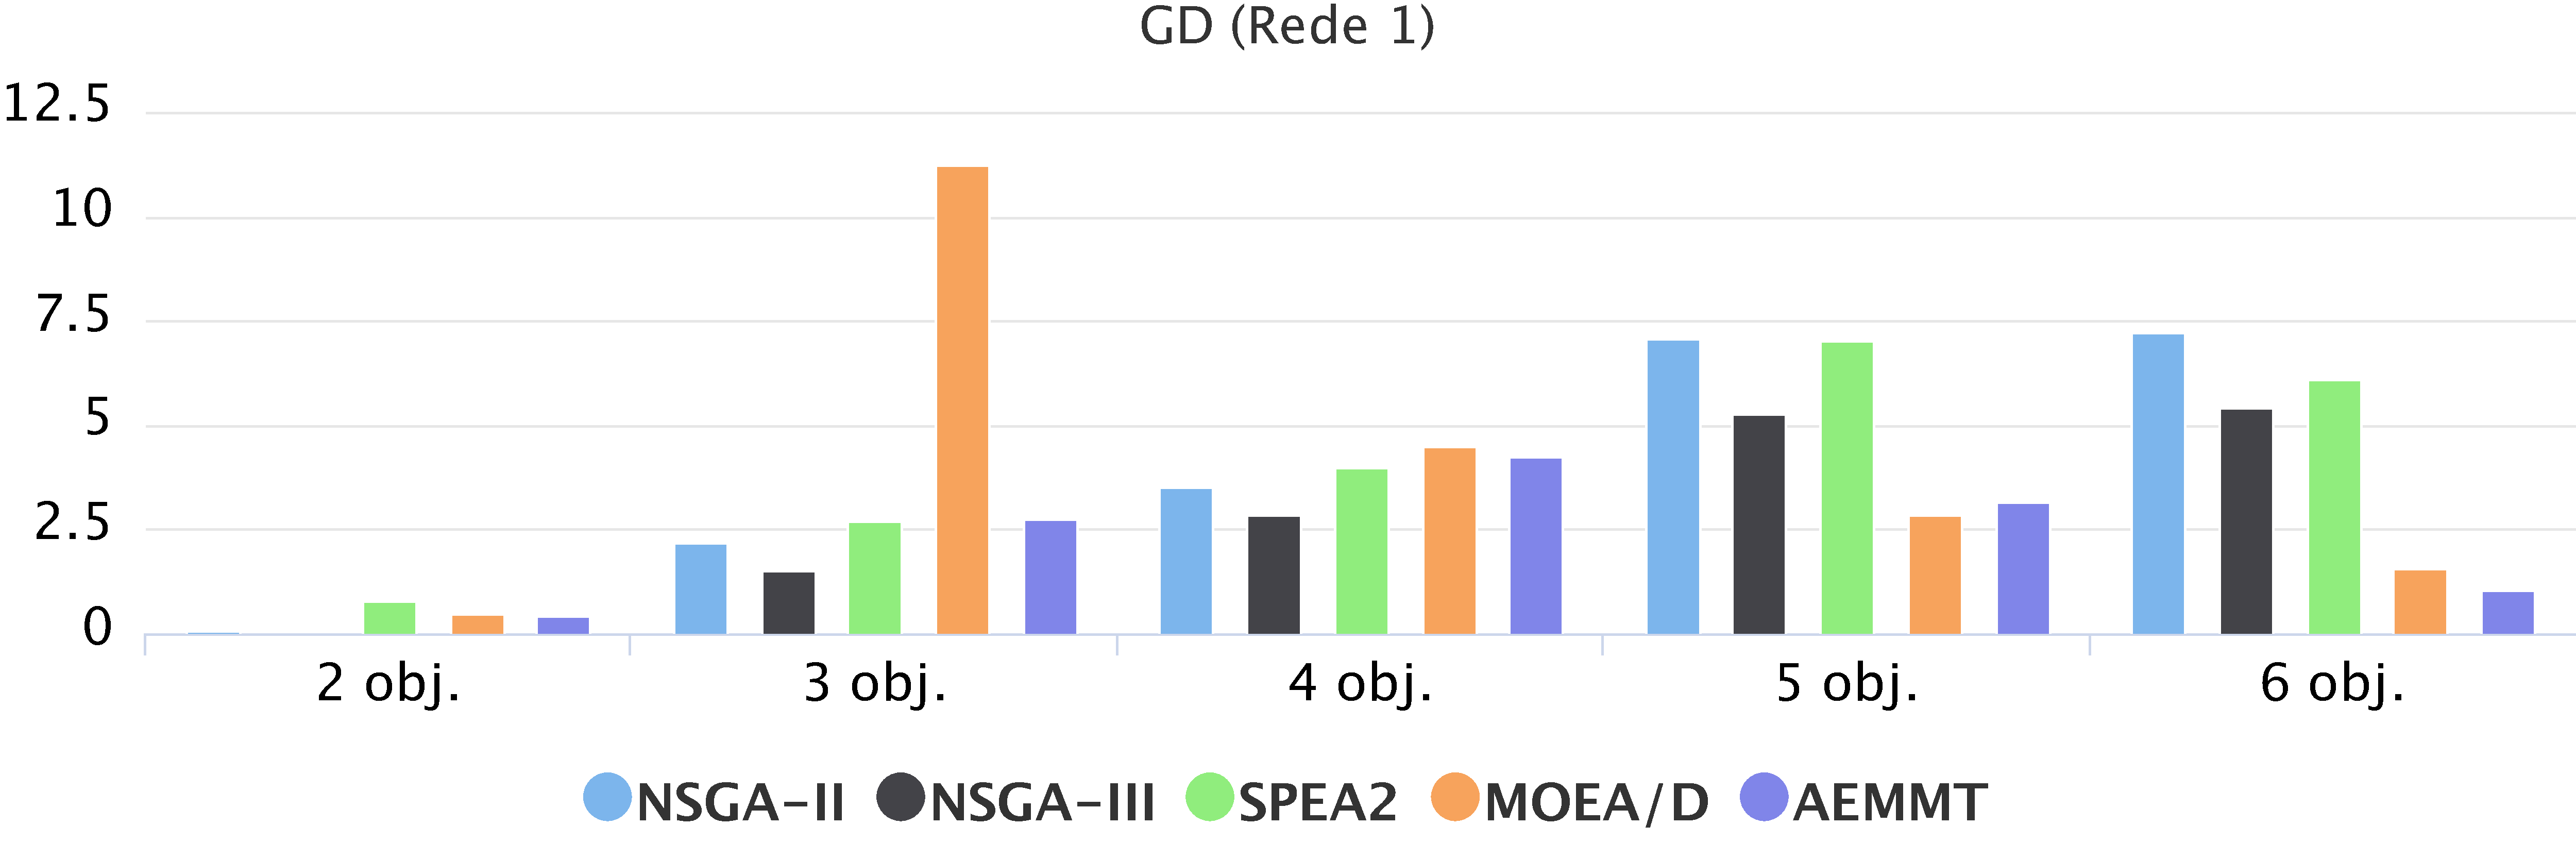
\includegraphics[width=1\textwidth]{cap_experimentos/figs/etapa1/gd-mrp-r1}
	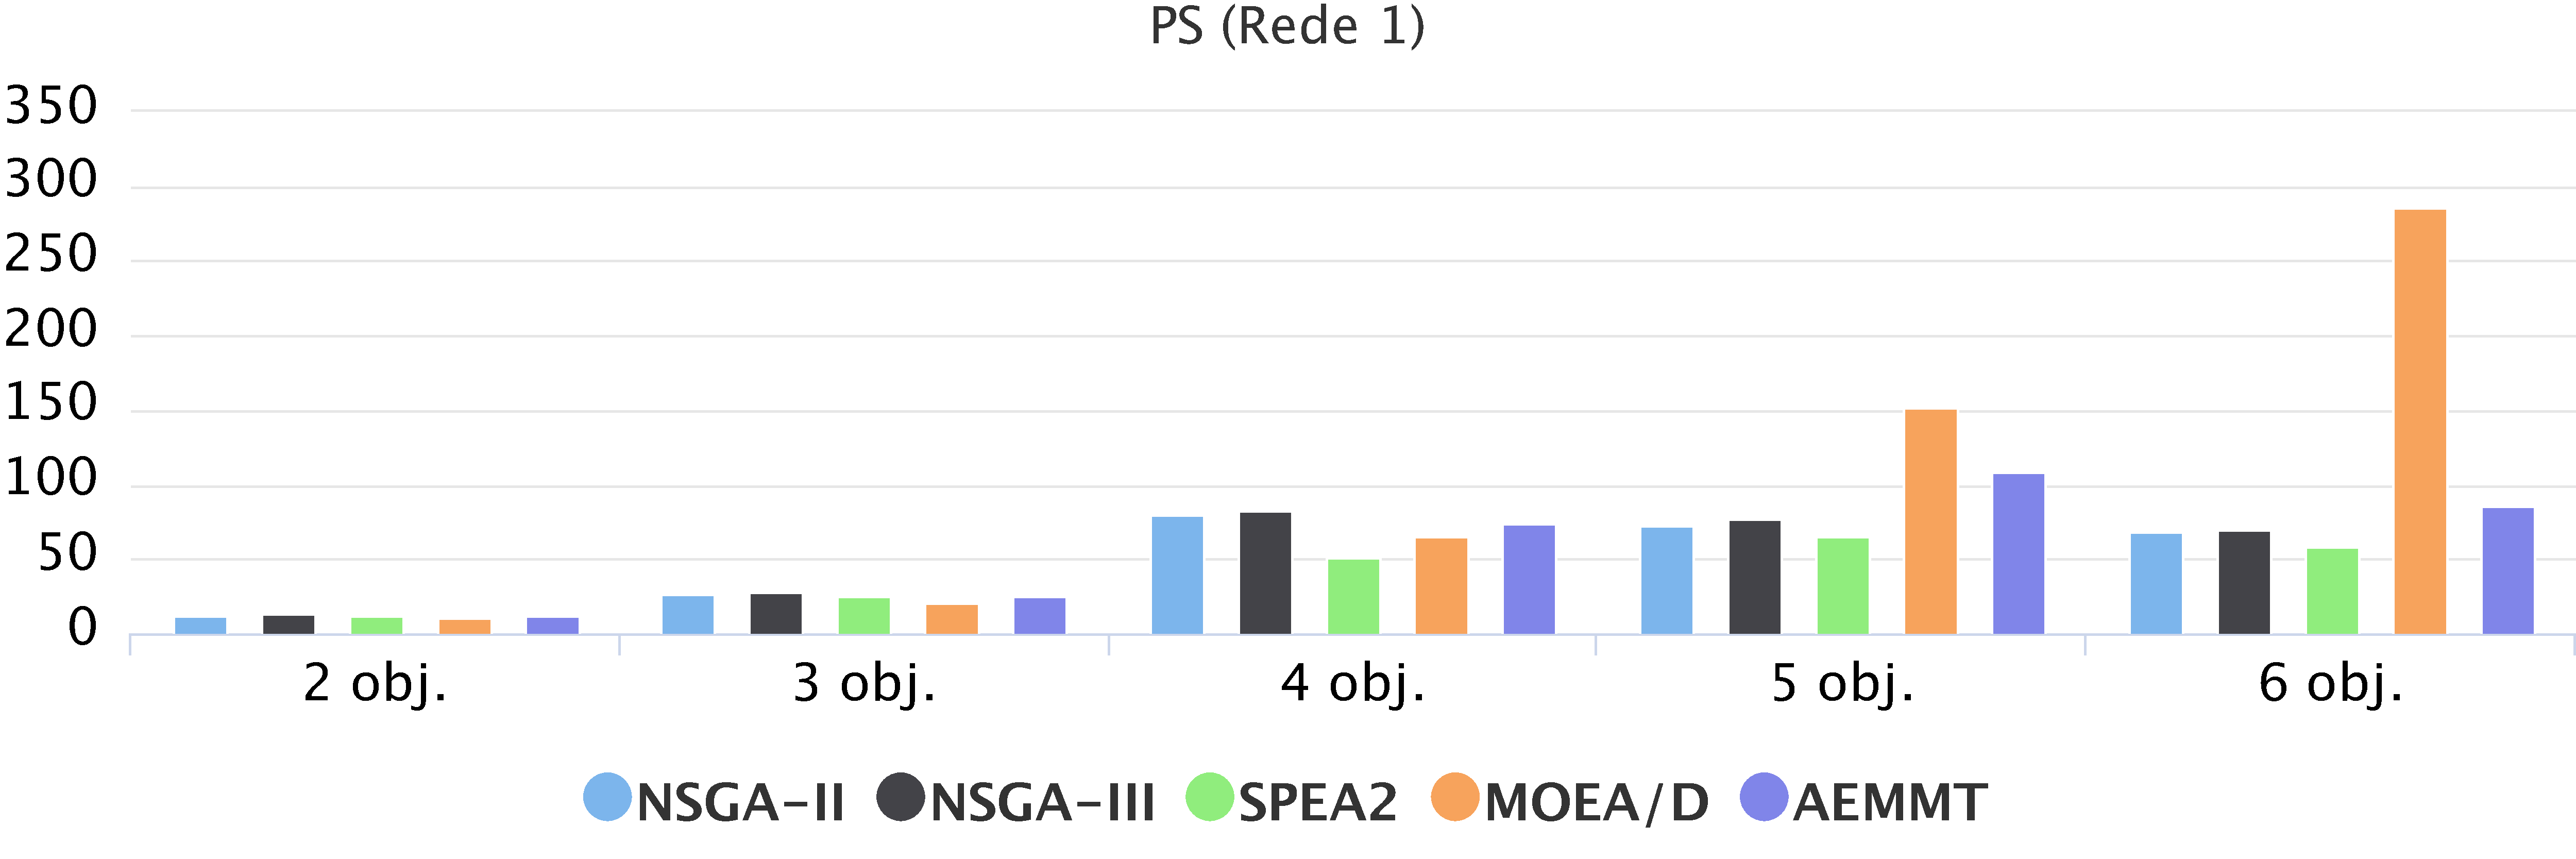
\includegraphics[width=1\textwidth]{cap_experimentos/figs/etapa1/ps-mrp-r1}
\end{figure*}

Análise do PRM-R1

\begin{figure*}[!htbp]
	\caption{Etapa 1: resultados para o PRM na rede $R_2$}
	\label{fig_exp1_mrp_r2}
	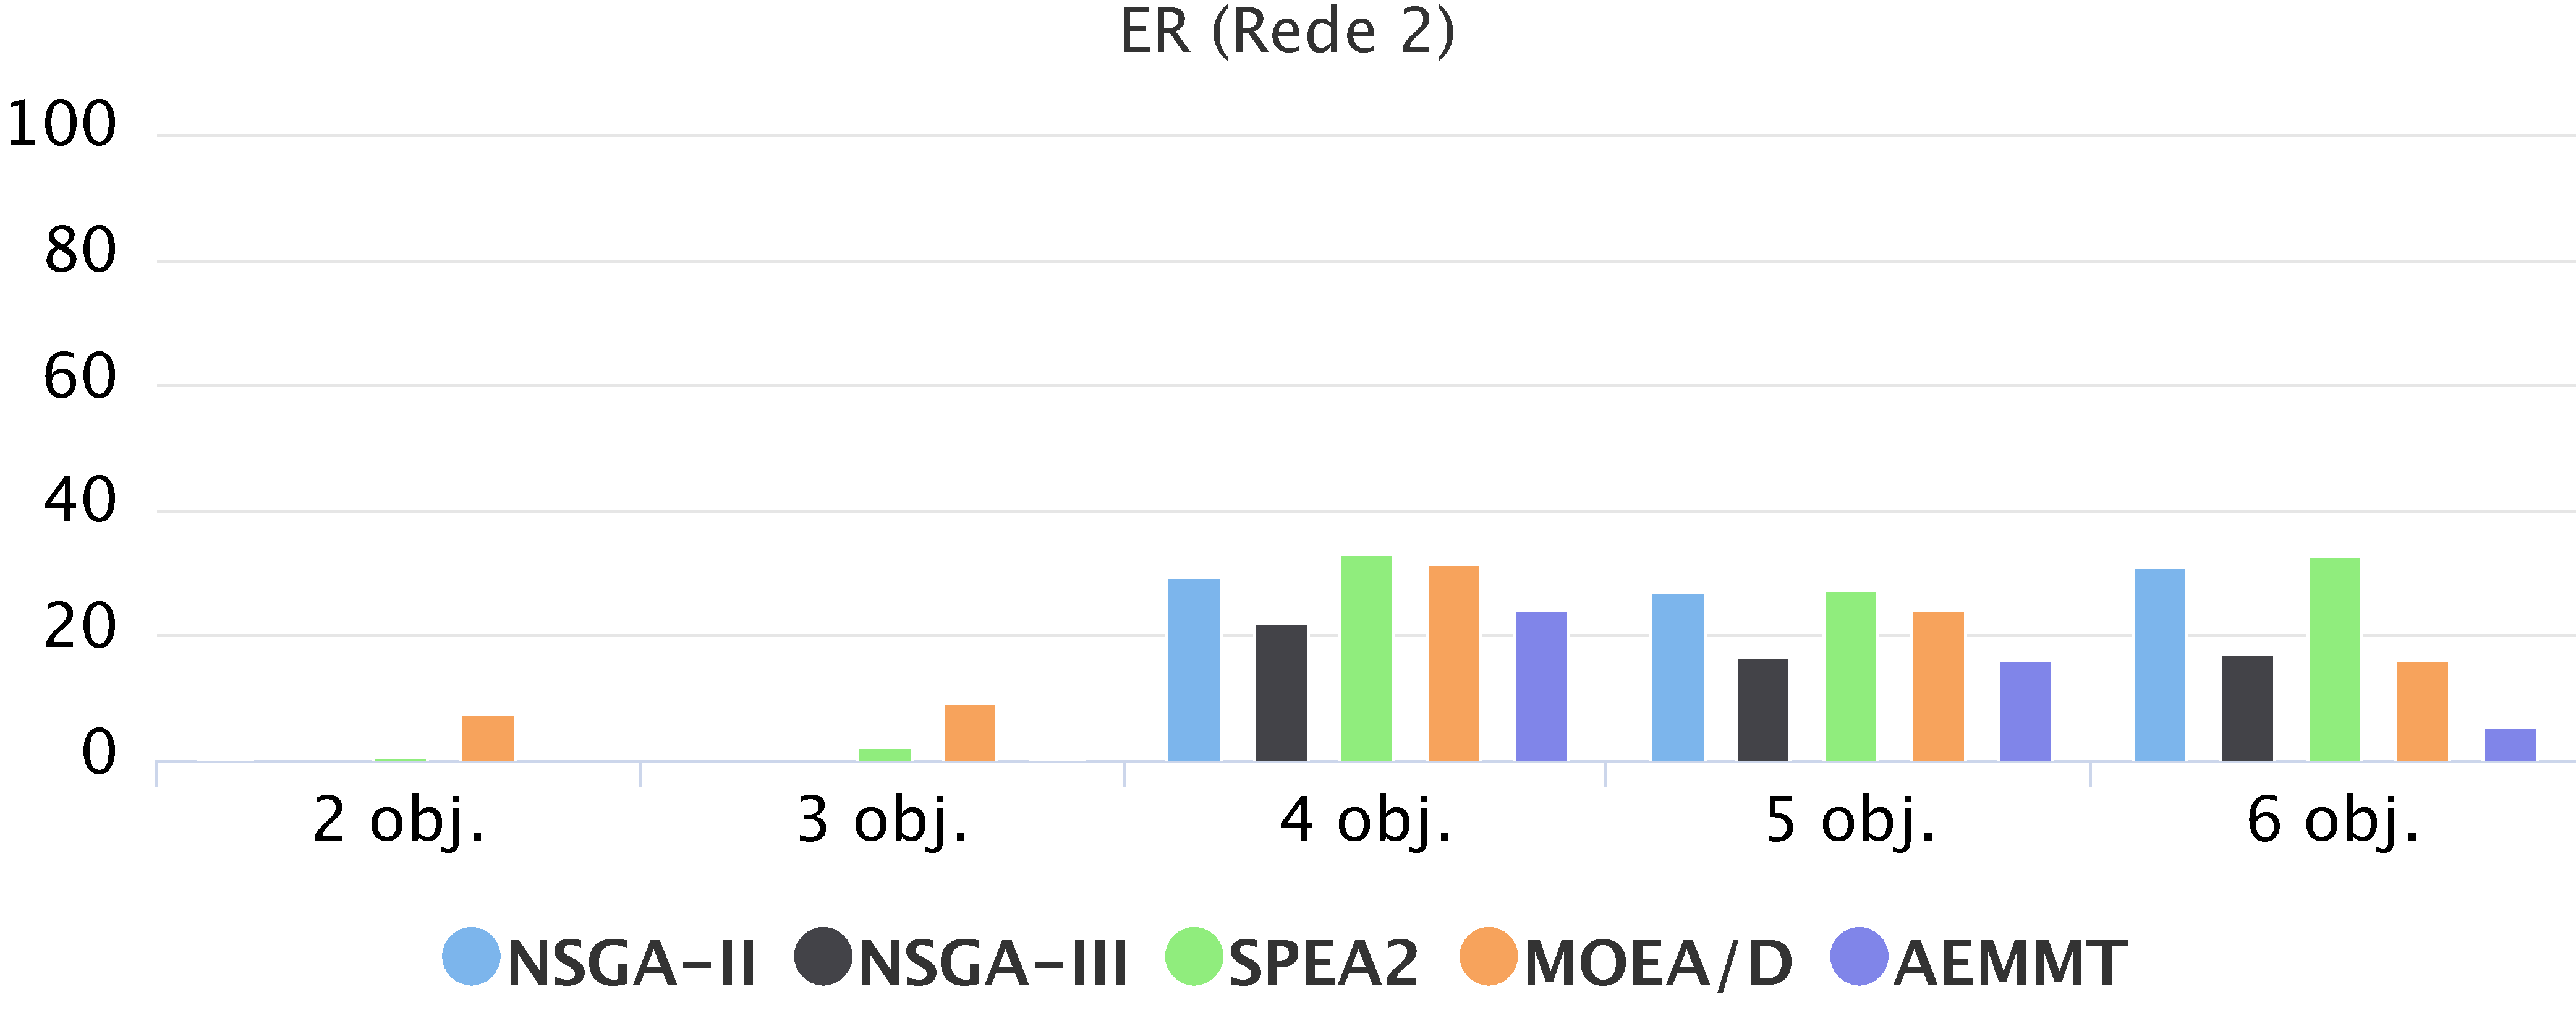
\includegraphics[width=1\textwidth]{cap_experimentos/figs/etapa1/er-mrp-r2}
	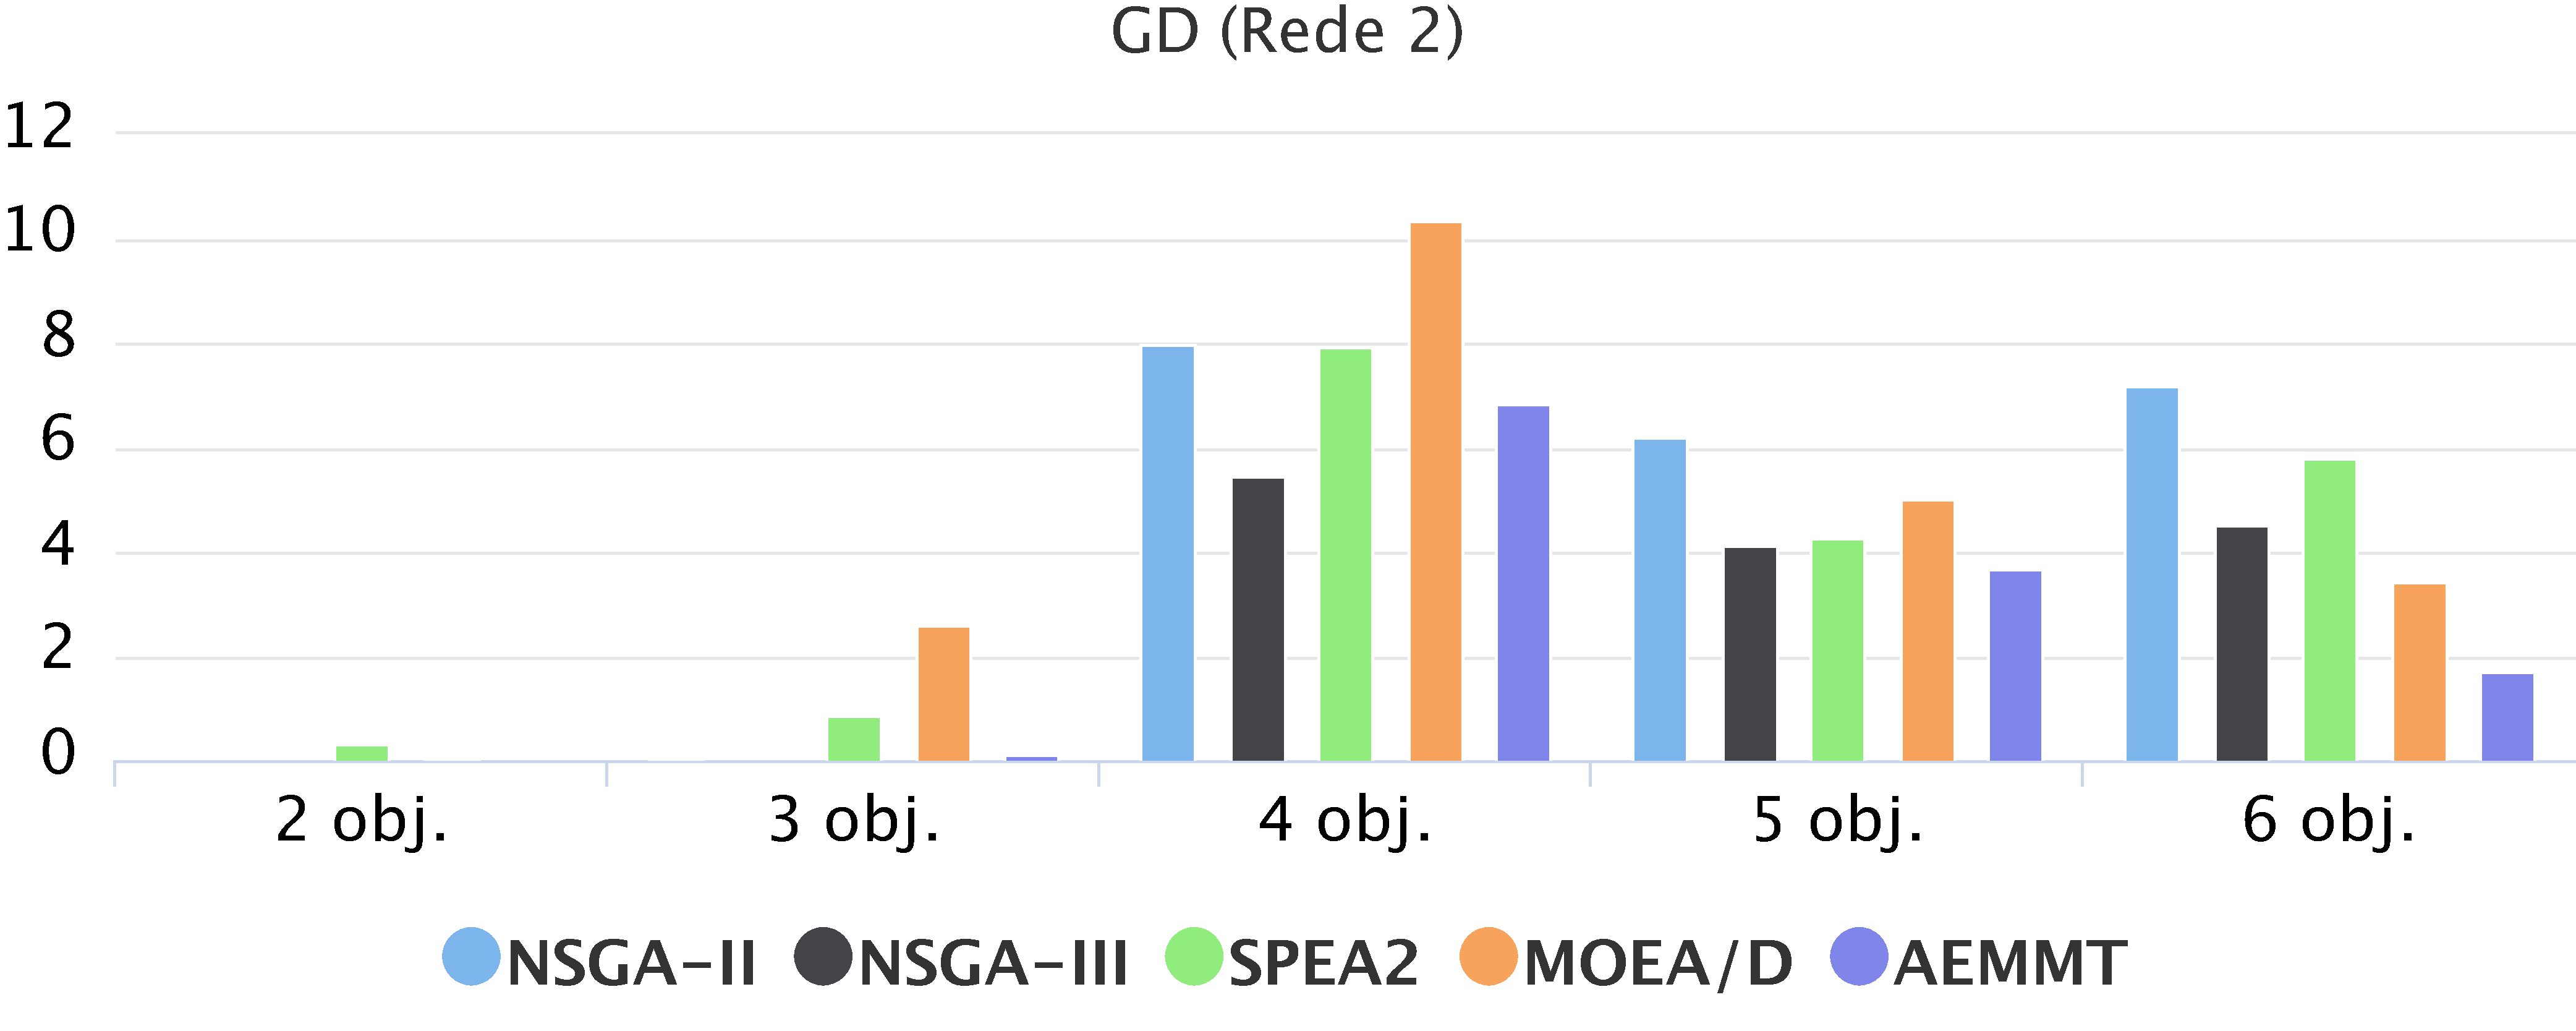
\includegraphics[width=1\textwidth]{cap_experimentos/figs/etapa1/gd-mrp-r2}
	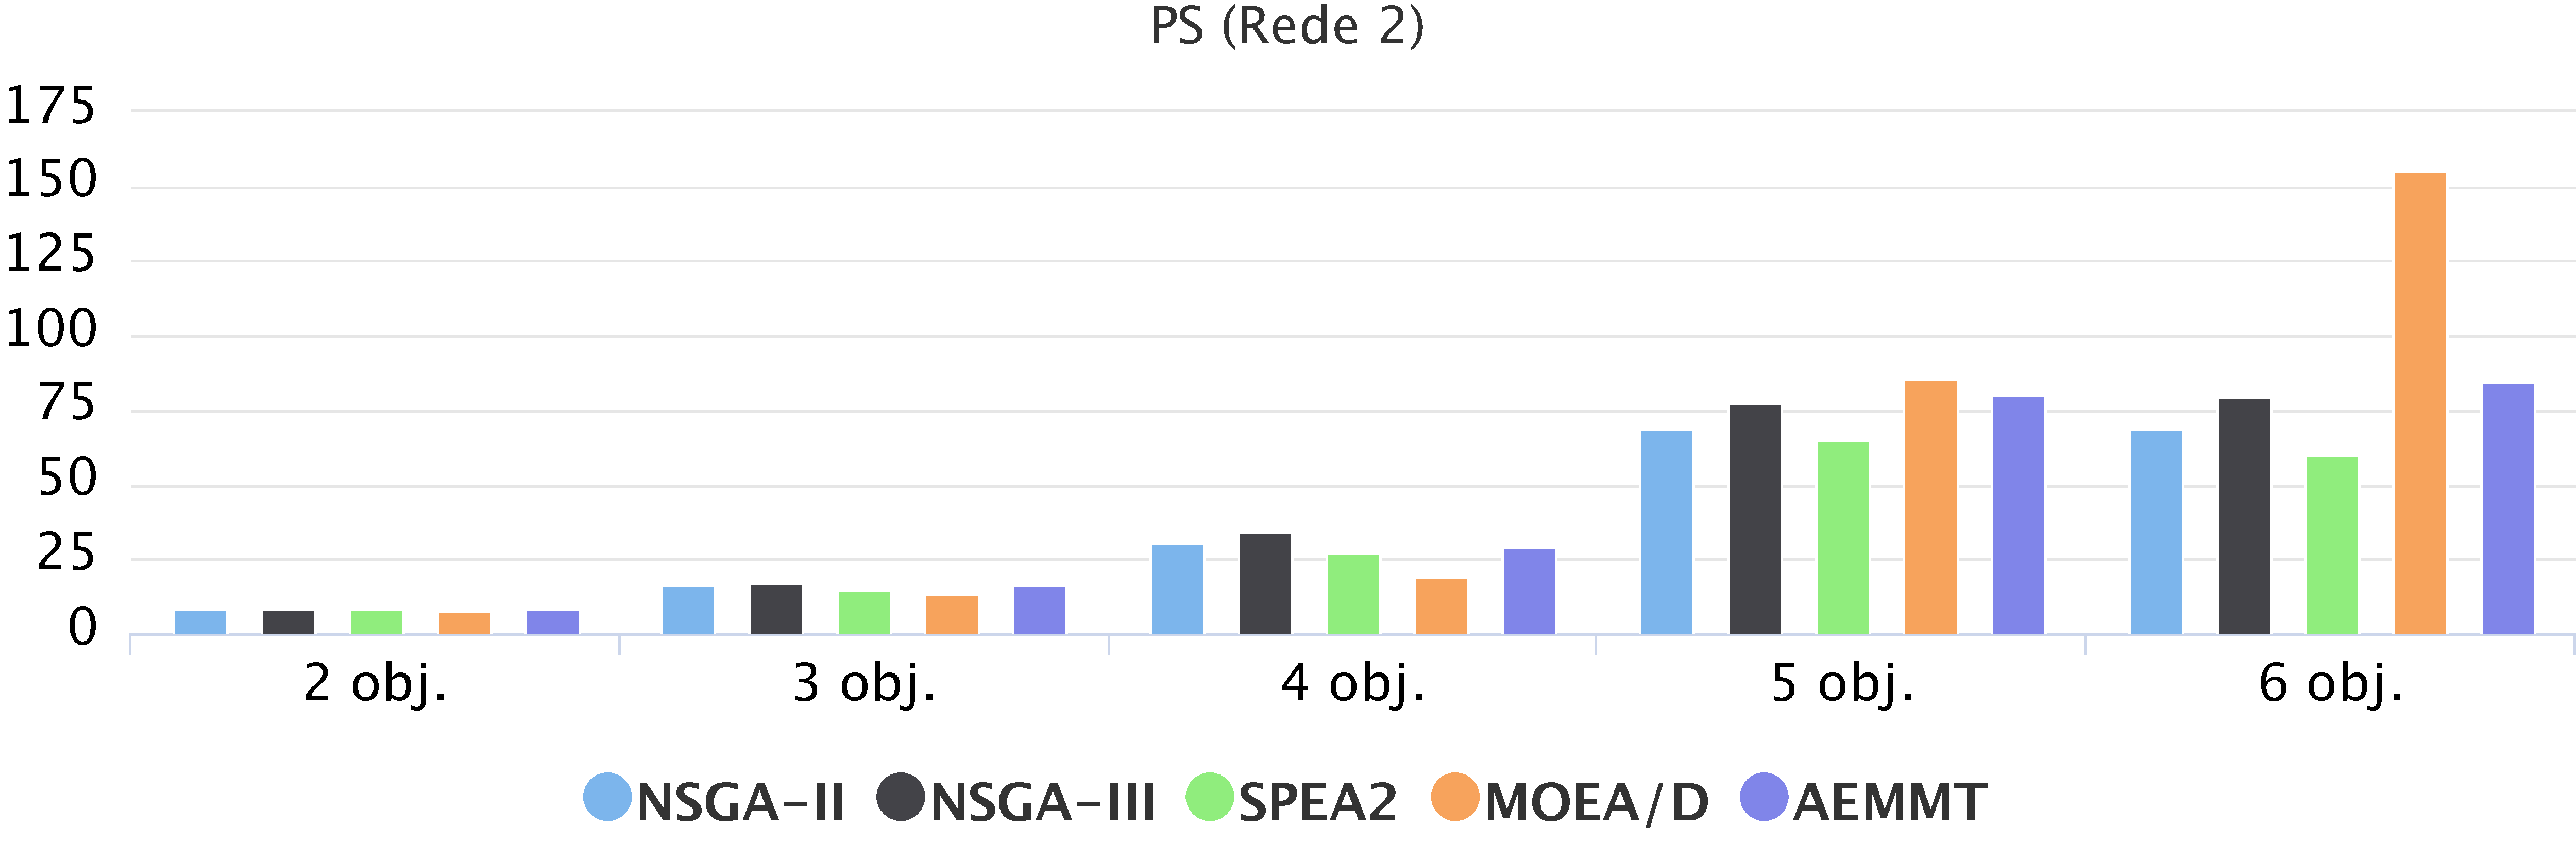
\includegraphics[width=1\textwidth]{cap_experimentos/figs/etapa1/ps-mrp-r2}
\end{figure*}

Análise do PRM-R2

\begin{figure*}[!htbp]
	\caption{Etapa 1: resultados para o PRM na rede $R_3$}
	\label{fig_exp1_mrp_r3}
	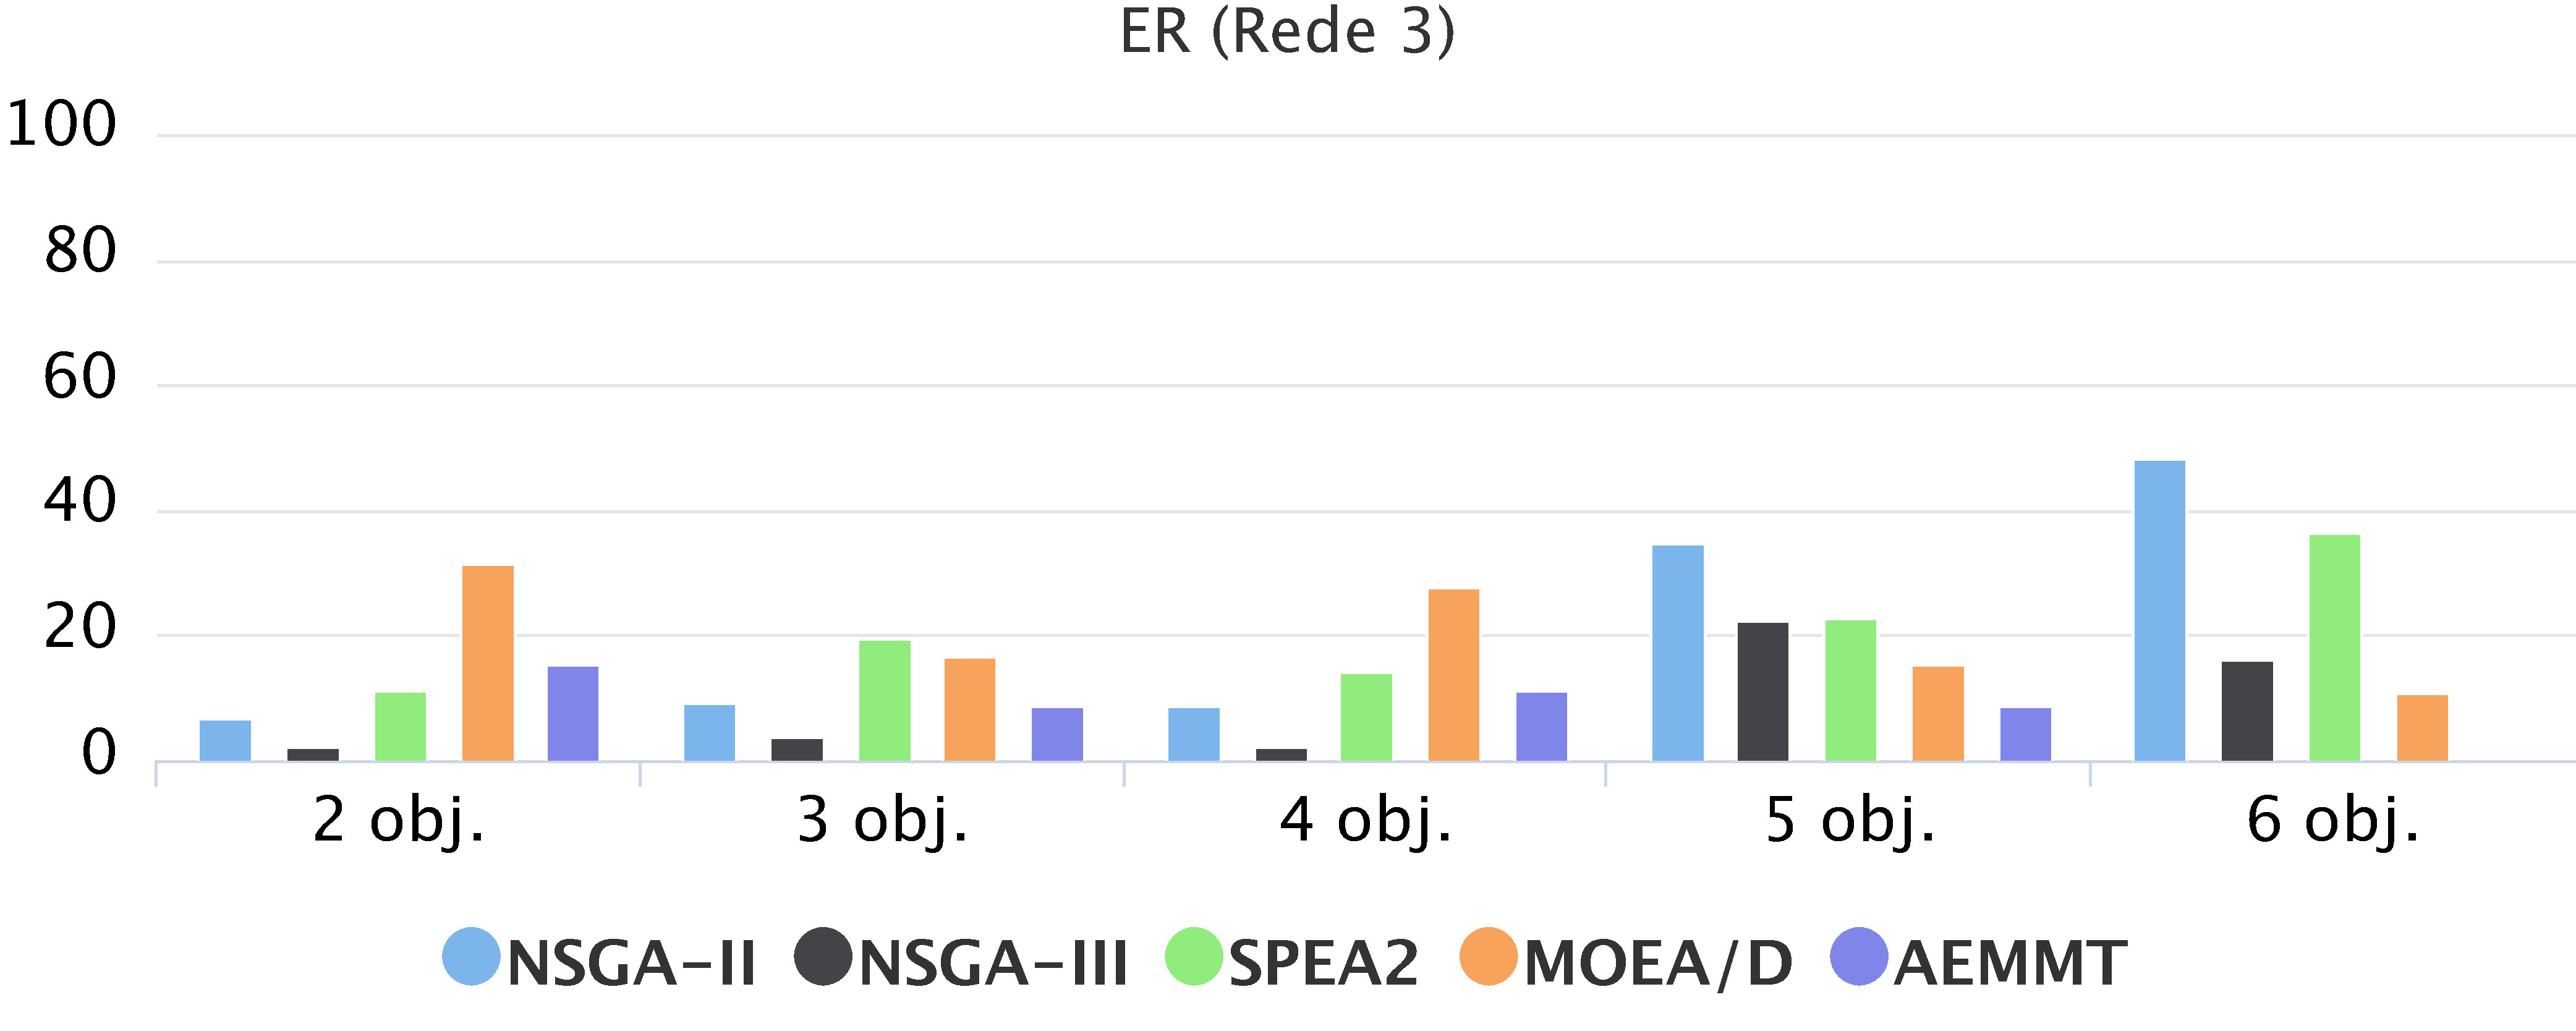
\includegraphics[width=1\textwidth]{cap_experimentos/figs/etapa1/er-mrp-r3}
	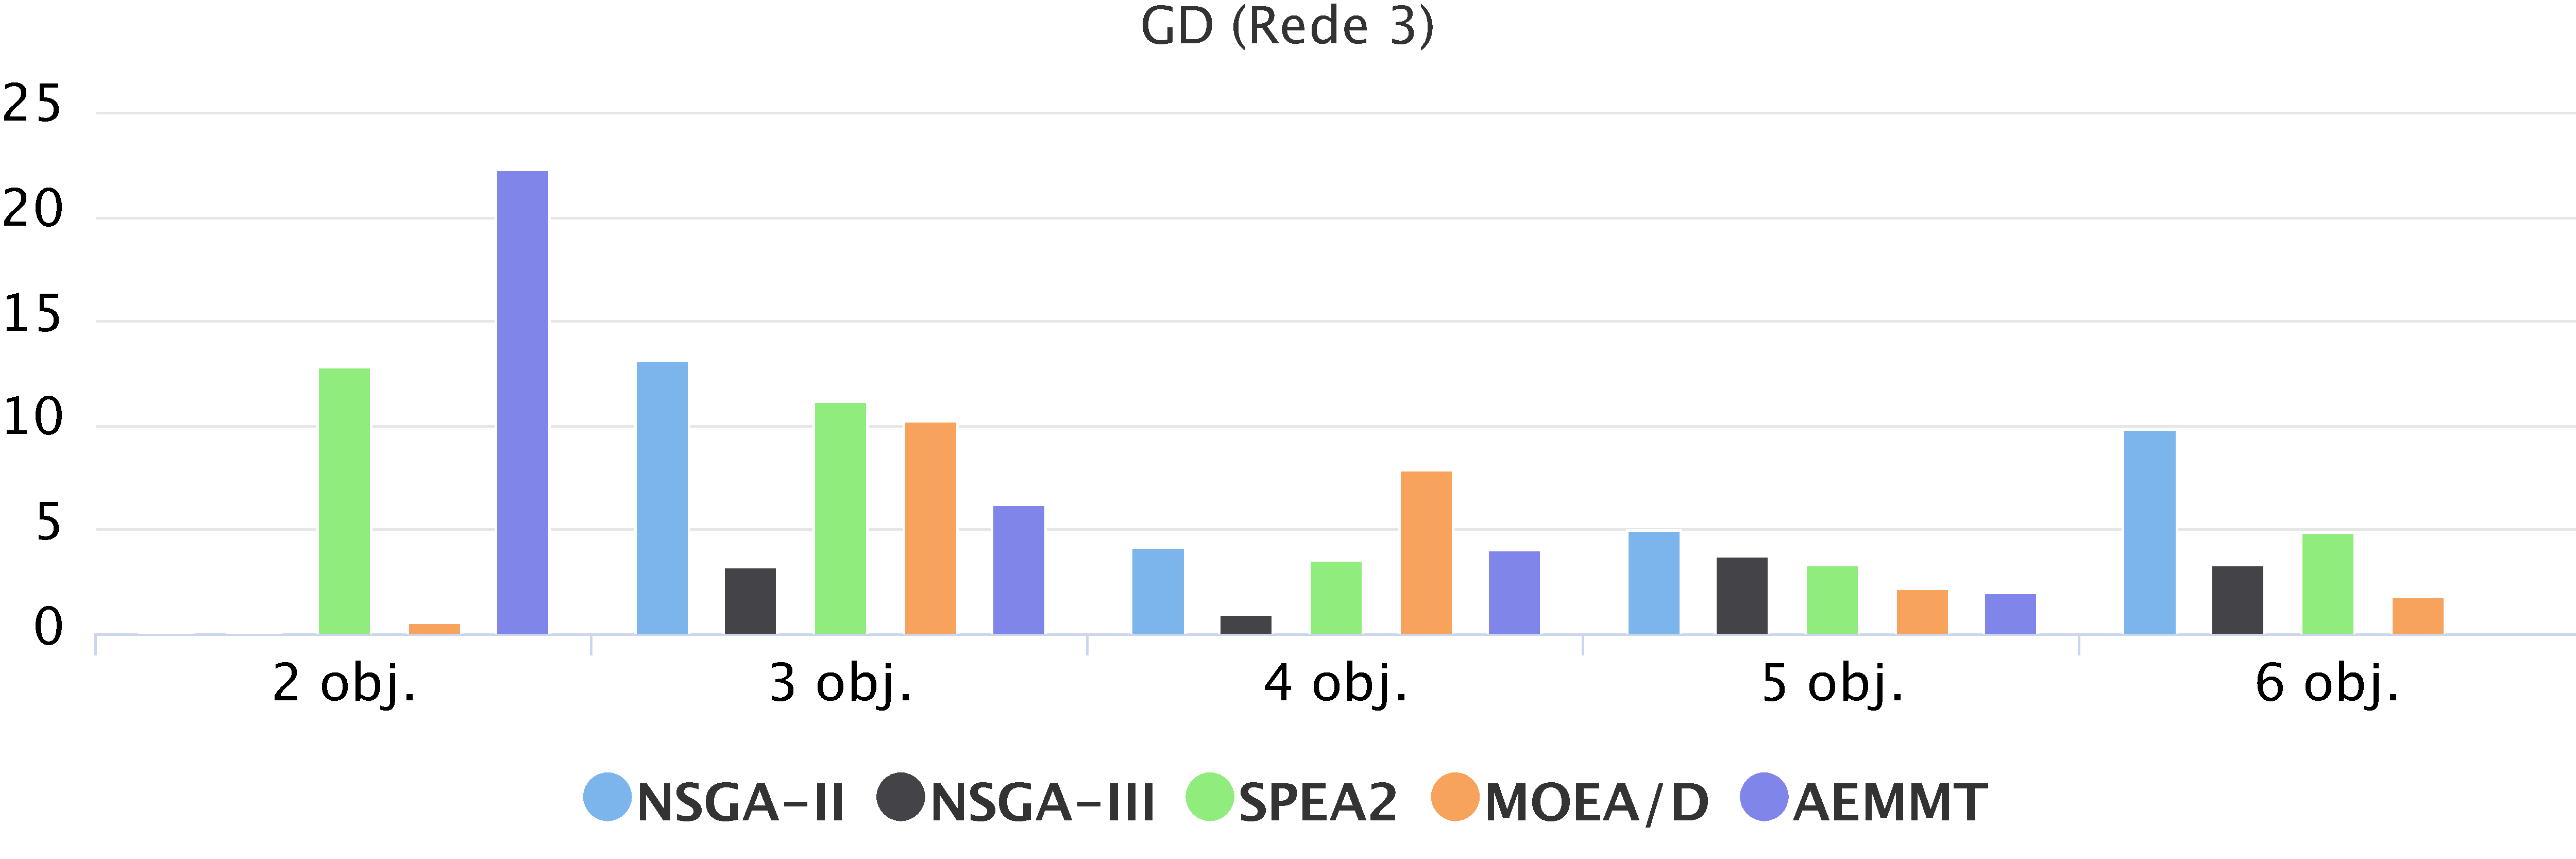
\includegraphics[width=1\textwidth]{cap_experimentos/figs/etapa1/gd-mrp-r3}
	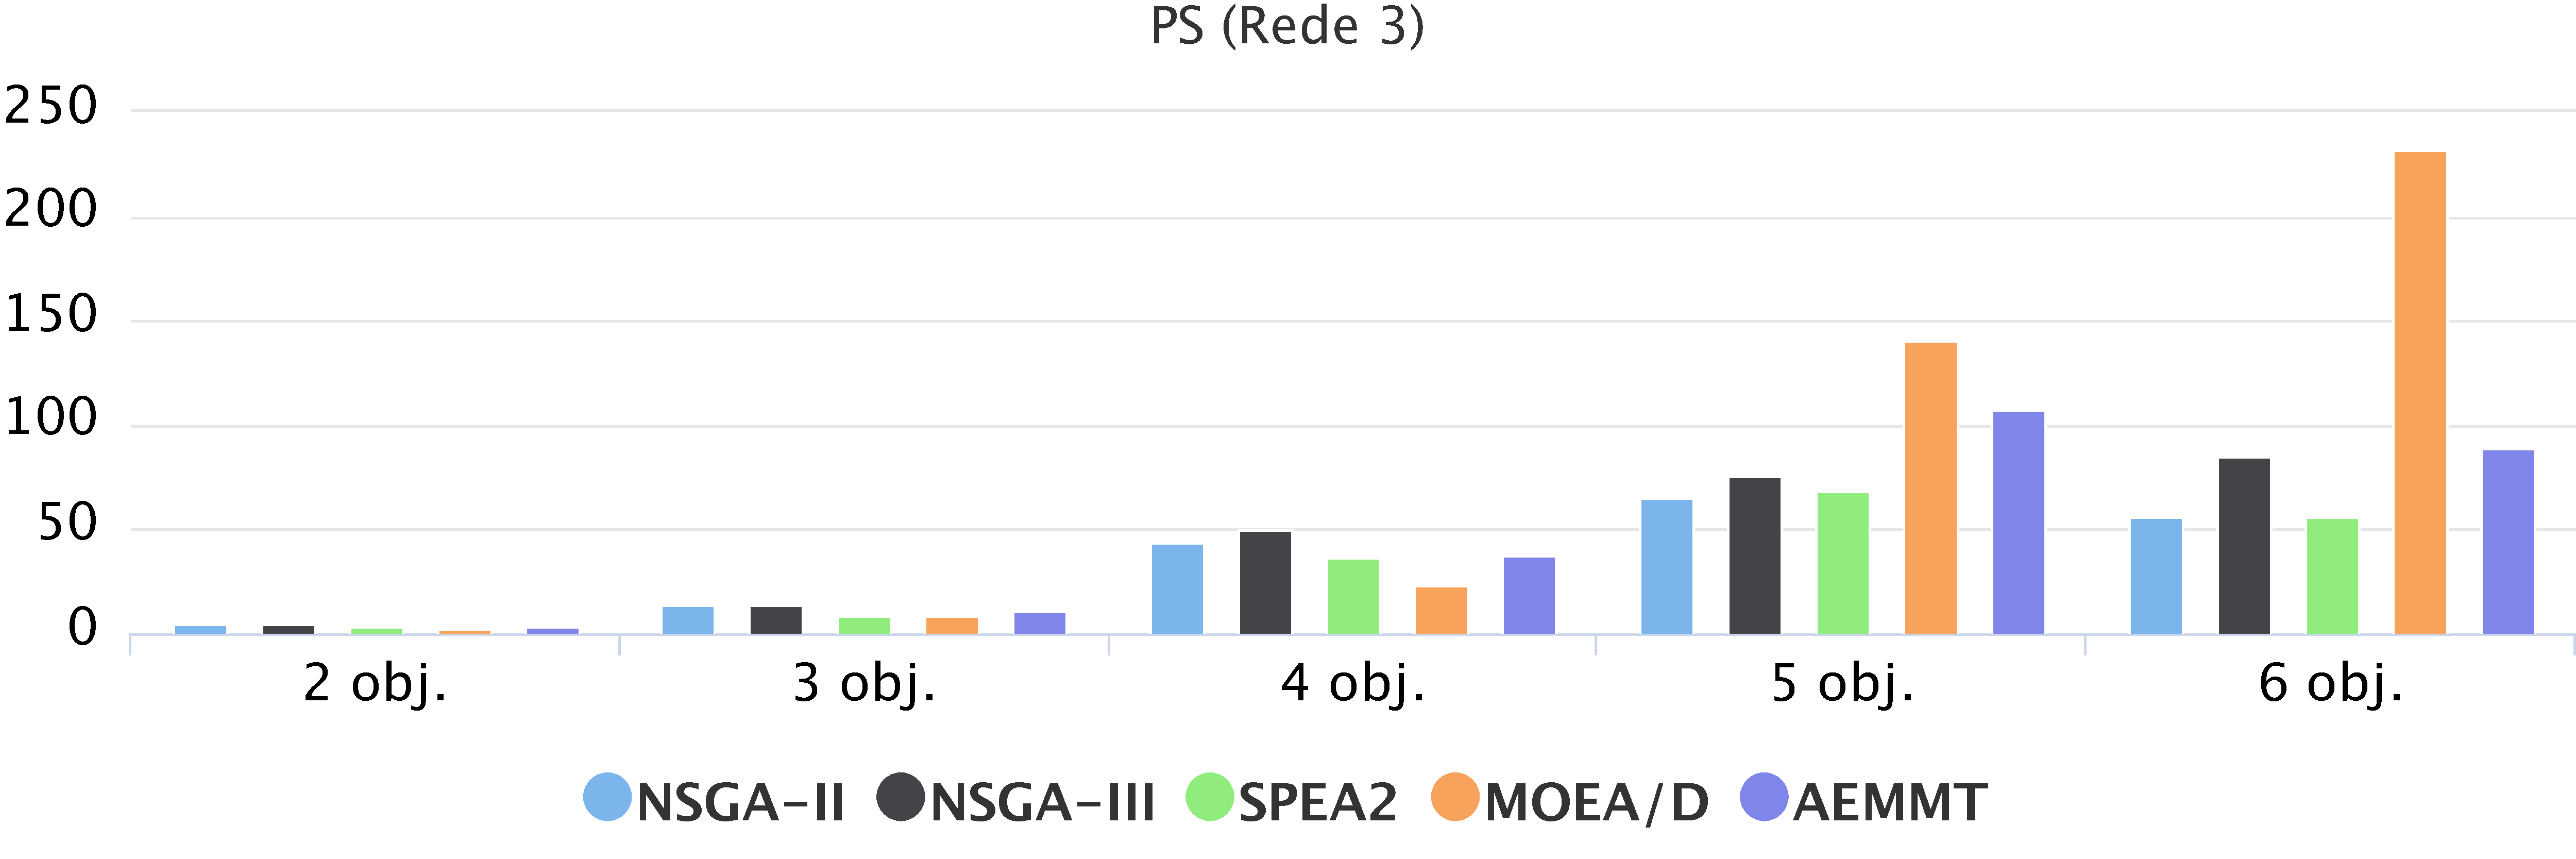
\includegraphics[width=1\textwidth]{cap_experimentos/figs/etapa1/ps-mrp-r3}
\end{figure*}

Análise do PRM-R3

\begin{figure*}[!htbp]
	\caption{Etapa 1: resultados agrupados para o PRM nas redes $R_1$, $R_2$ e $R_3$}
	\label{fig_exp1_mrp_todos}
	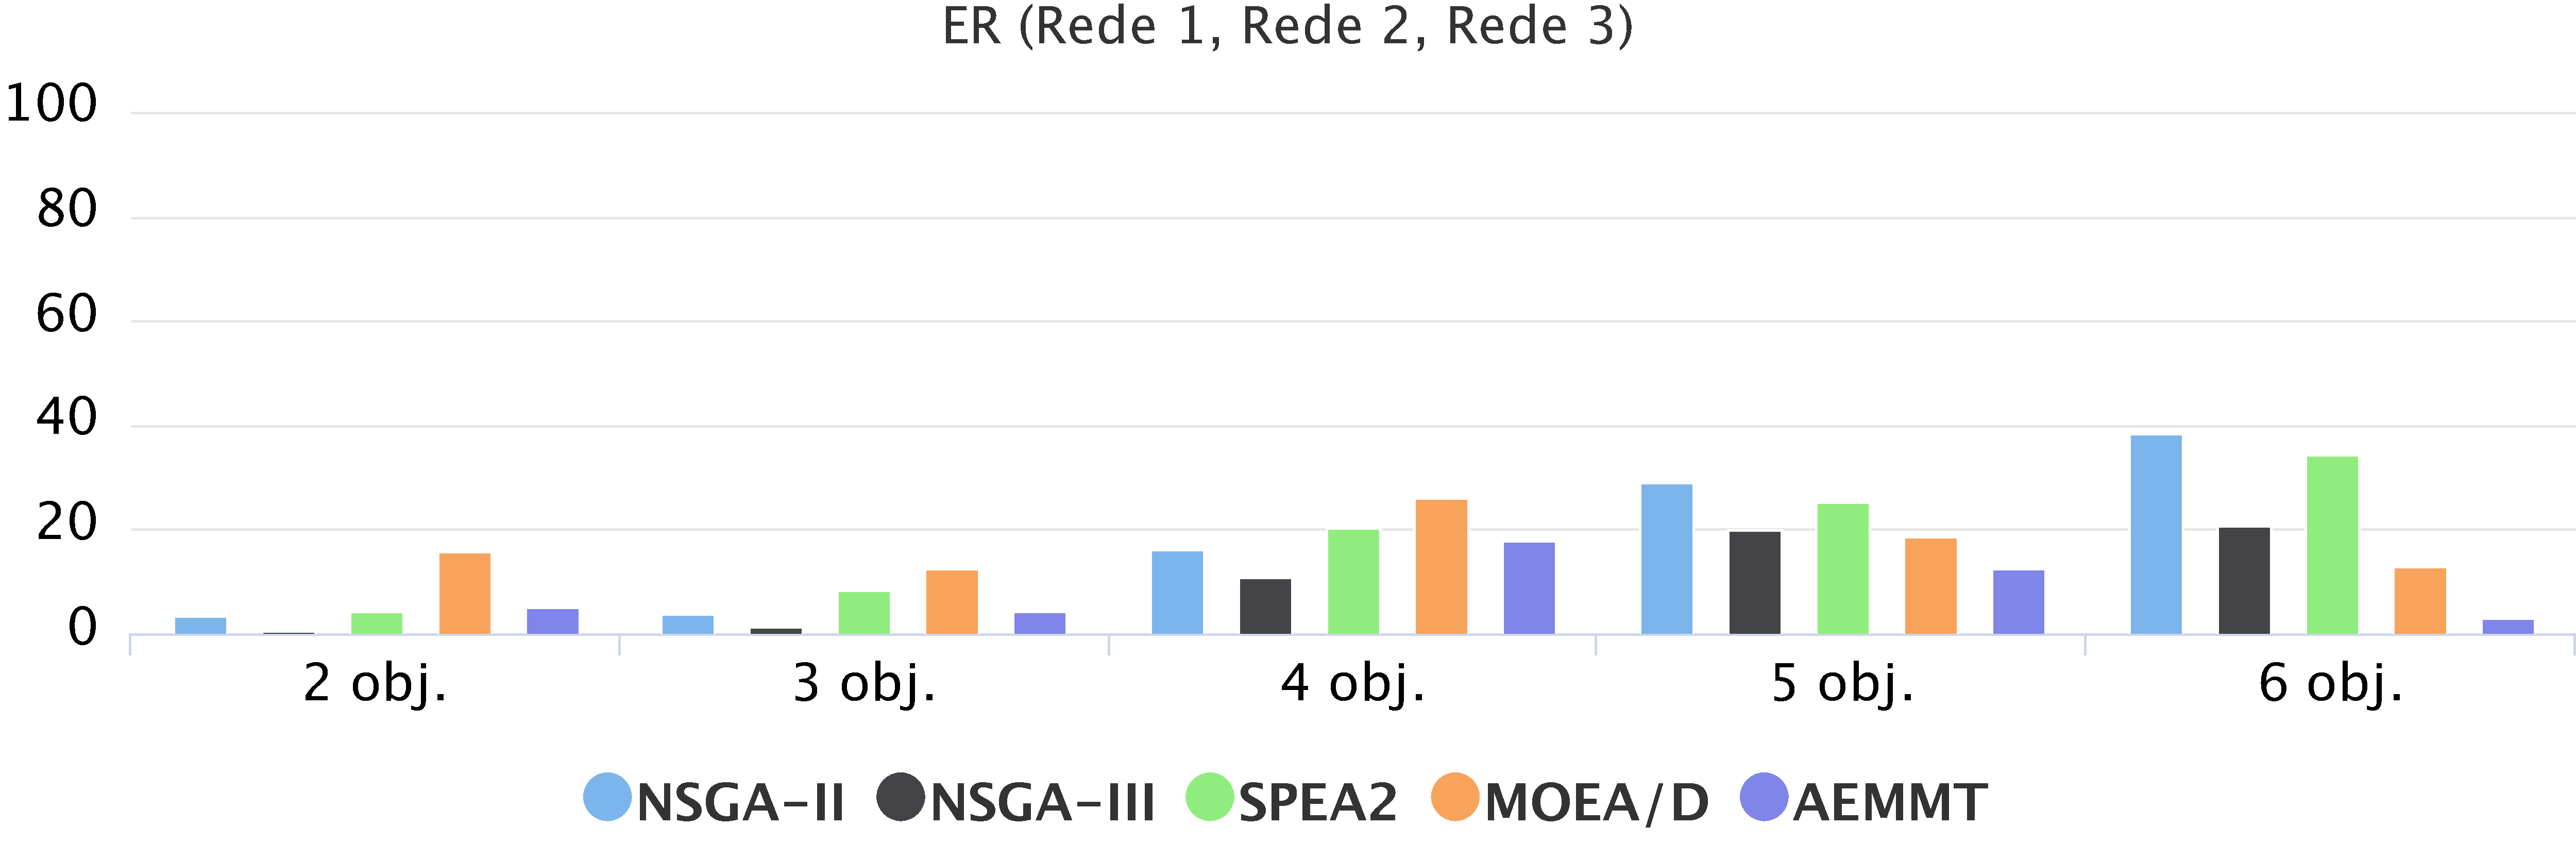
\includegraphics[width=1\textwidth]{cap_experimentos/figs/etapa1/er-mrp-todos}
	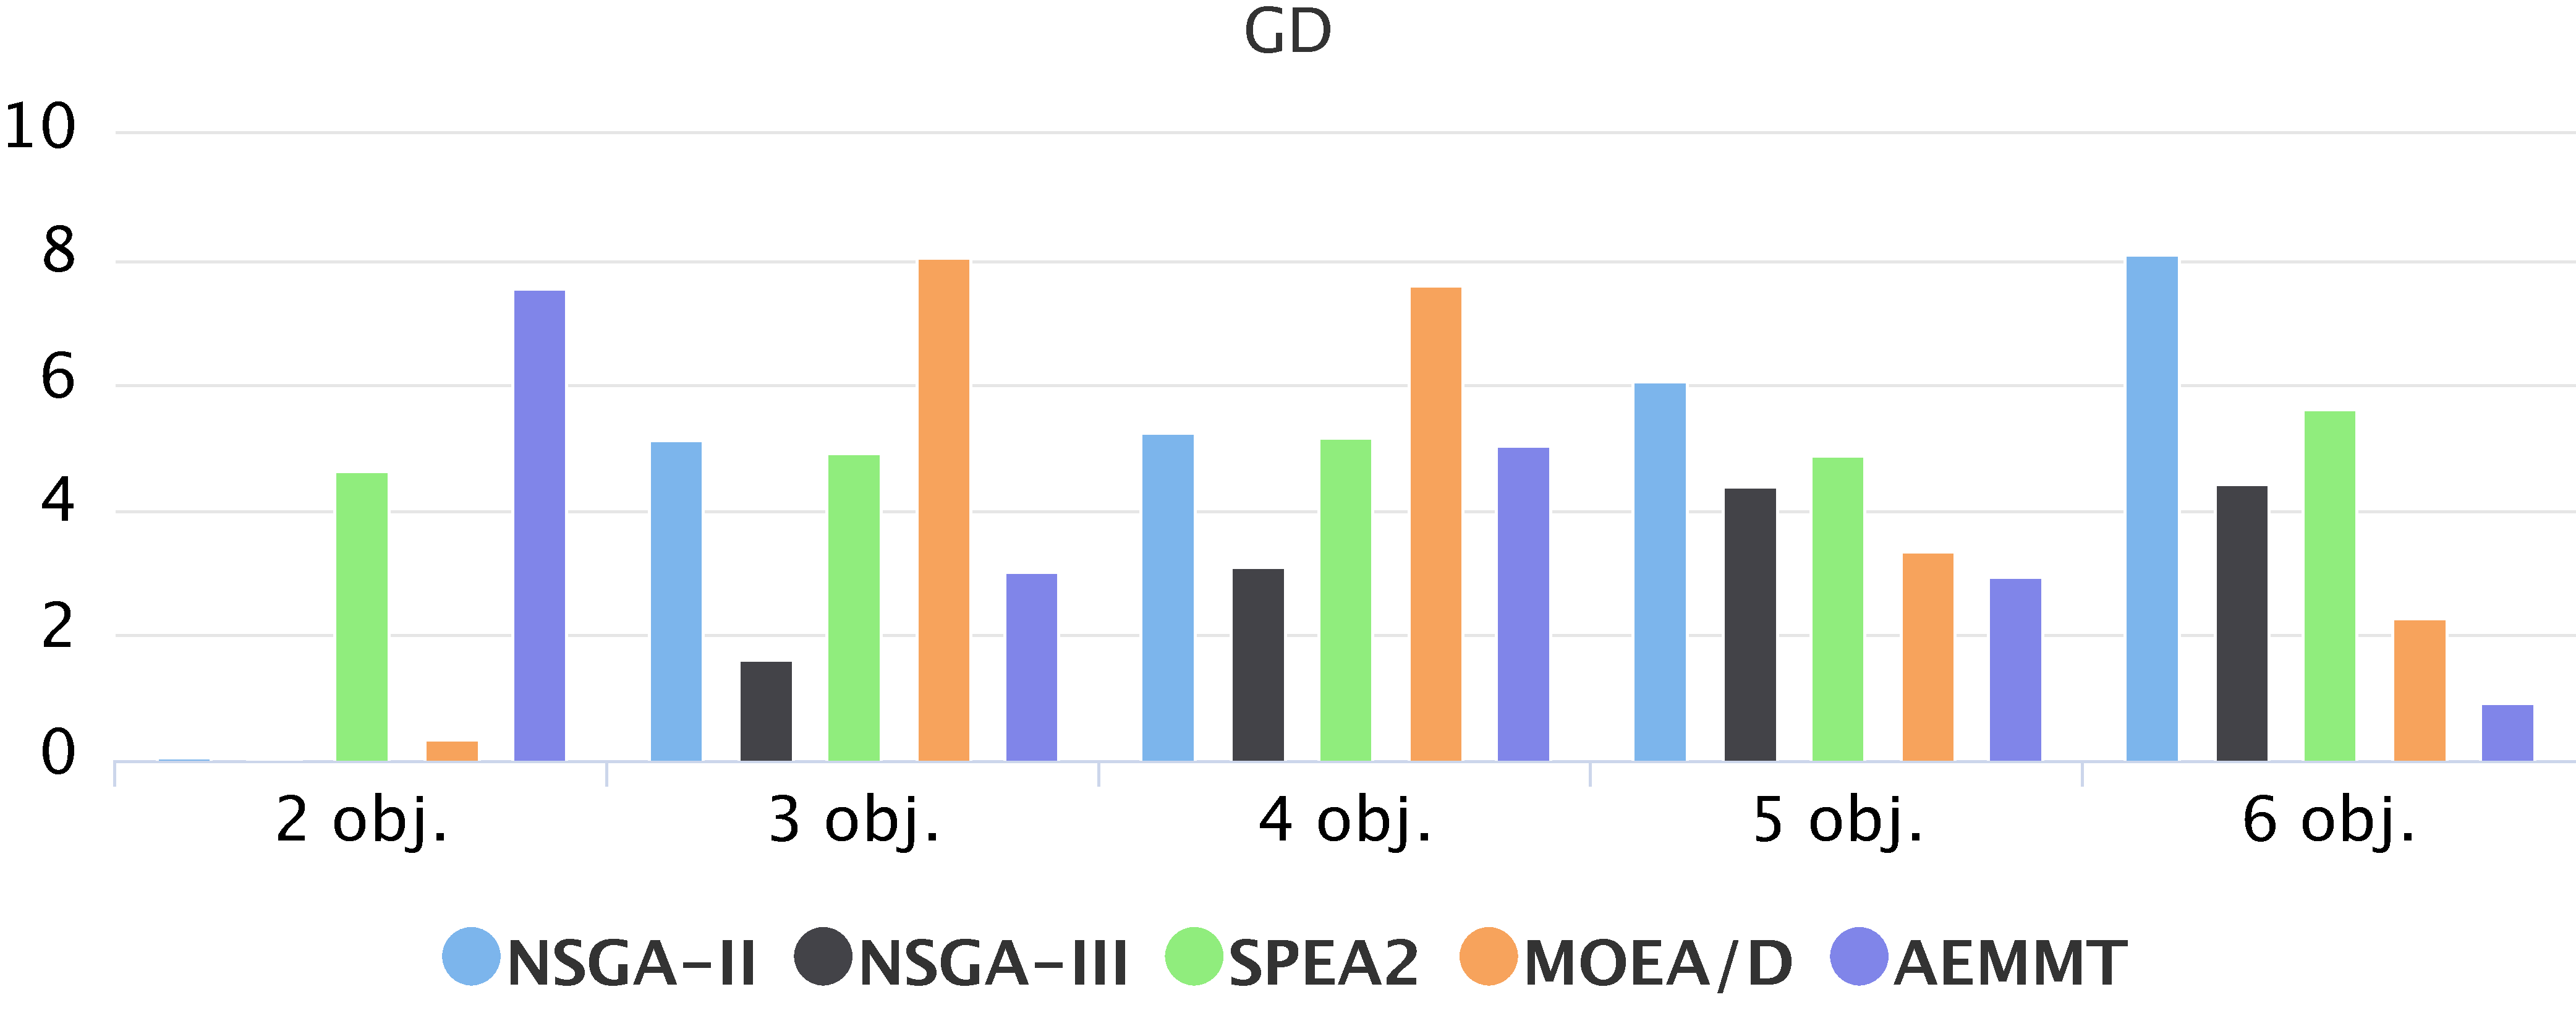
\includegraphics[width=1\textwidth]{cap_experimentos/figs/etapa1/gd-mrp-todos}
	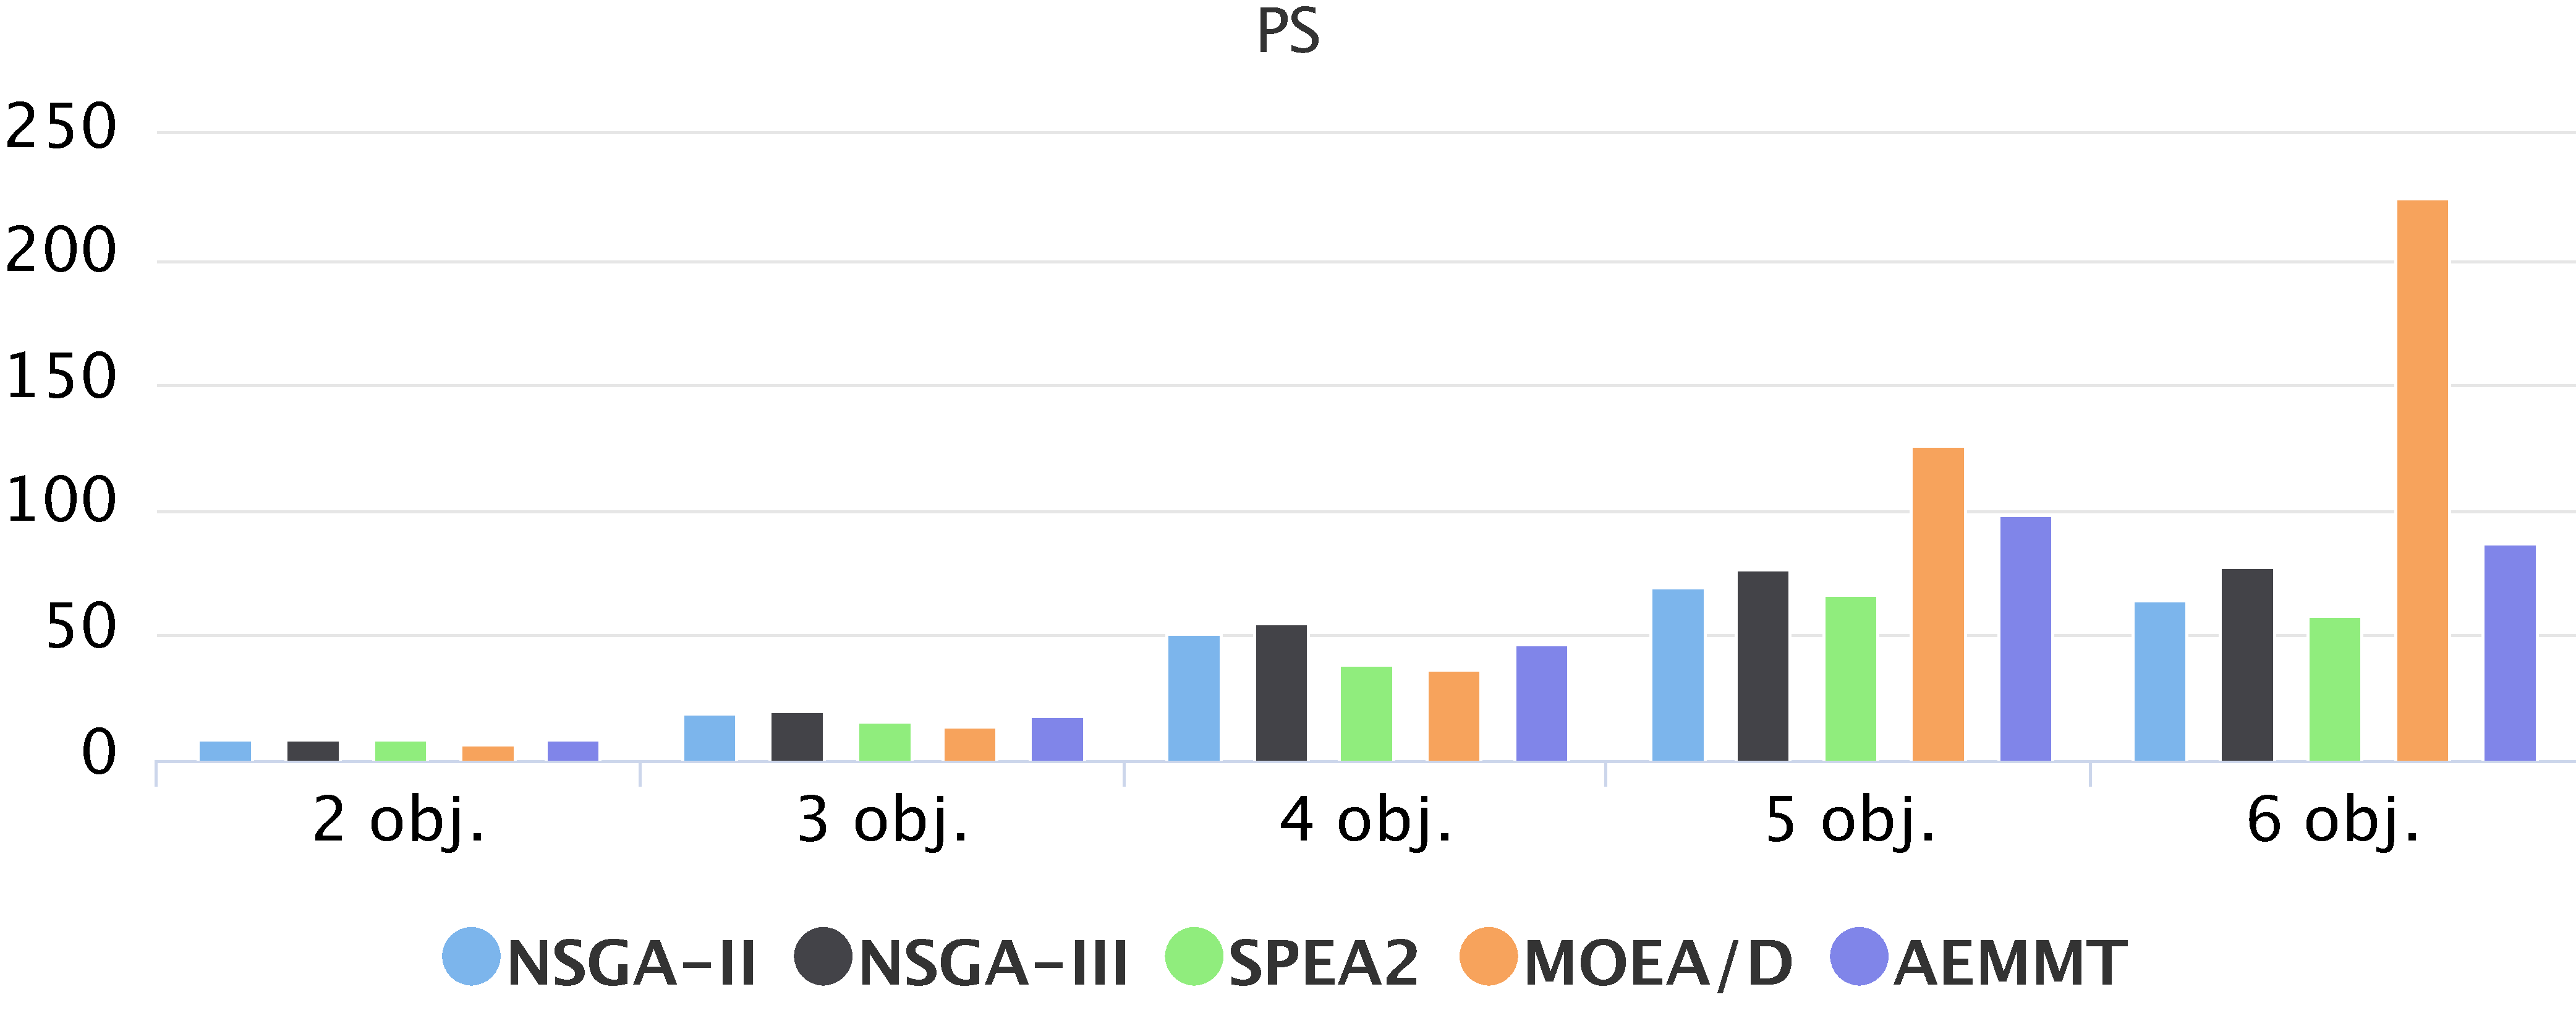
\includegraphics[width=1\textwidth]{cap_experimentos/figs/etapa1/ps-mrp-todos}
\end{figure*}

Análise geral do PRM

Análise geral dos resultados comparando os dois problemas.

\section{Etapa 2: AG's many-objectives vs. MACO/D}

Na segunda etapa de experimentos descartam-se os AEMOs clássicos NSGA-II e SPEA2 e inclui-se o AEMMD e o MACO/D, algoritmo proposto neste trabalho. Uma nova métrica de desempenho é utilizada, o tempo, e as demais continuam sendo o erro ($ER$), a distância ($GD$) e o número de soluções corretas ($PS$). Assim como na etapa 1, o Pareto aproximado foi pré-calculado a partir de múltiplas execuções dos algoritmos e é apresentado na tabela \ref{table_exp2_paretos}. Enfim, os resultados foram obtidos através das médias entre 100 execuções dos 30 cenários descritos na lista a seguir.

\begin{itemize}
	\item PRM: 5 formulações de objetivos ($P_4$, $P_5$ e $P_6$) e 3 redes ($R_1$, $R_2$ e $R_3$). Tanto as formulações quanto às redes foram descritas na seção correspondente ao problema do roteamento multicast [].
	\item PMM: 5 formulações de objetivos (4 a 6) e 3 instâncias (30, 40 e 50 itens).
\end{itemize}


\begin{table}[!htbp]
	\centering
	\caption{Cardinalidade dos Paretos encontrados para a primeira etapa de experimentos}
	\label{table_exp2_paretos}
	\begin{tabular}{c|rrr|rrr}
		& \multicolumn{3}{c|}{\textbf{PRM}} & \multicolumn{3}{c}{\textbf{PMM}} \\ \hline
		Objetivos & R1         & R2       & R3        & 30 itens  & 50 itens & 100 itens \\ \hline
		2         & 14         & 9        & 6         & 15        & 67       & 170       \\
		3         & 30         & 18       & 17        & 106       & 501      & 6288      \\
		4         & 122        & 72       & 60        & 425       & 986      & 88374*    \\
		5         & 424        & 326      & 551       & 1765      & 5213     & 176868*   \\
		6         & 1196       & 657      & 1078      & 5800      & 35760*   & 248198*   \\ \hline
	\end{tabular}
\end{table}

A tabela \ref{table_exp2_parametros} apresenta os parâmetros dos algoritmos utilizados neste experimento. Note que o número de gerações (marcado com asterisco) deve ser multiplicado pelo tamanho da população no AEMMT e AEMMD devido ao fato de realizarem apenas um crossover por geração.

\begin{table}[!htbp]
	\caption{Parâmetros utilizados para o PRM e o PMM.}
	\label{table_exp2_parametros}
	\begin{center}
		\begin{tabular}{c|r|r}
			\textbf{Parâmetro} & \textbf{PRM} &  \textbf{PMM} \\ %\hline
			\hline
			Tamanho da população               &    90 &      150 \\ %\hline
			Número de gerações*        &   100 &      100 \\ %\hline
			Taxa de crossover                & 100\% &    100\% \\ %\hline
			Taxa de mutação                 &  20\% &      5\% \\ %\hline
			Tamanho da vizinhança (MOEA/D)    &    10 &       10 \\ %\hline
			Tamanho das tabelas (MEAMT)   &    30 &       50 \\ %\hline
			Tamanho da tabela de dominância (MEAMT) &    90 &      150 \\ %\hline
			Número de divisões (NSGA-III)&     8 &        8 \\ %\hline
			$\alpha, \beta, \rho$ (MACO/D)& 1, 2, 0.3 & 1, 4.3, 0.3 \\ %\hline
			Intervalo de valores para os feromônios (MACO/D)& [0.1, 0.9] & [0.1, 0.9] \\ %\hline
			Tamanho das amostras (MACO/D)& 10 &25\% of the number of items \\  %\hline
			Tamanho do grupo de estruturas ativas (MACO/D)& 5 & 5 \\
			\hline
		\end{tabular}
	\end{center}
\end{table}

As figuras \ref{fig_exp2_pmm_30}, \ref{fig_exp2_pmm_40} e \ref{fig_exp2_pmm_50} mostram respectivamente os resultados para o PMM de 30, 40 e 50 itens. As figuras \ref{fig_exp2_prm_r1}, \ref{fig_exp2_prm_r2} e \ref{fig_exp2_prm_r3} revelam respectivamente os resultados para o PRM aplicado às redes $R_1$, $R_2$ e $R_3$. Uma análise conjunta, com uma média entre as três instâncias de cada problema é apresenta nas figuras \ref{fig_exp2_prm_todos} (PRM) e \ref{fig_exp2_pmm_todos} (PMM).

\begin{figure*}[!htbp]
	\caption{Etapa 2: resultados para o PMM com 30 itens}
	\label{fig_exp2_mkp_30}
	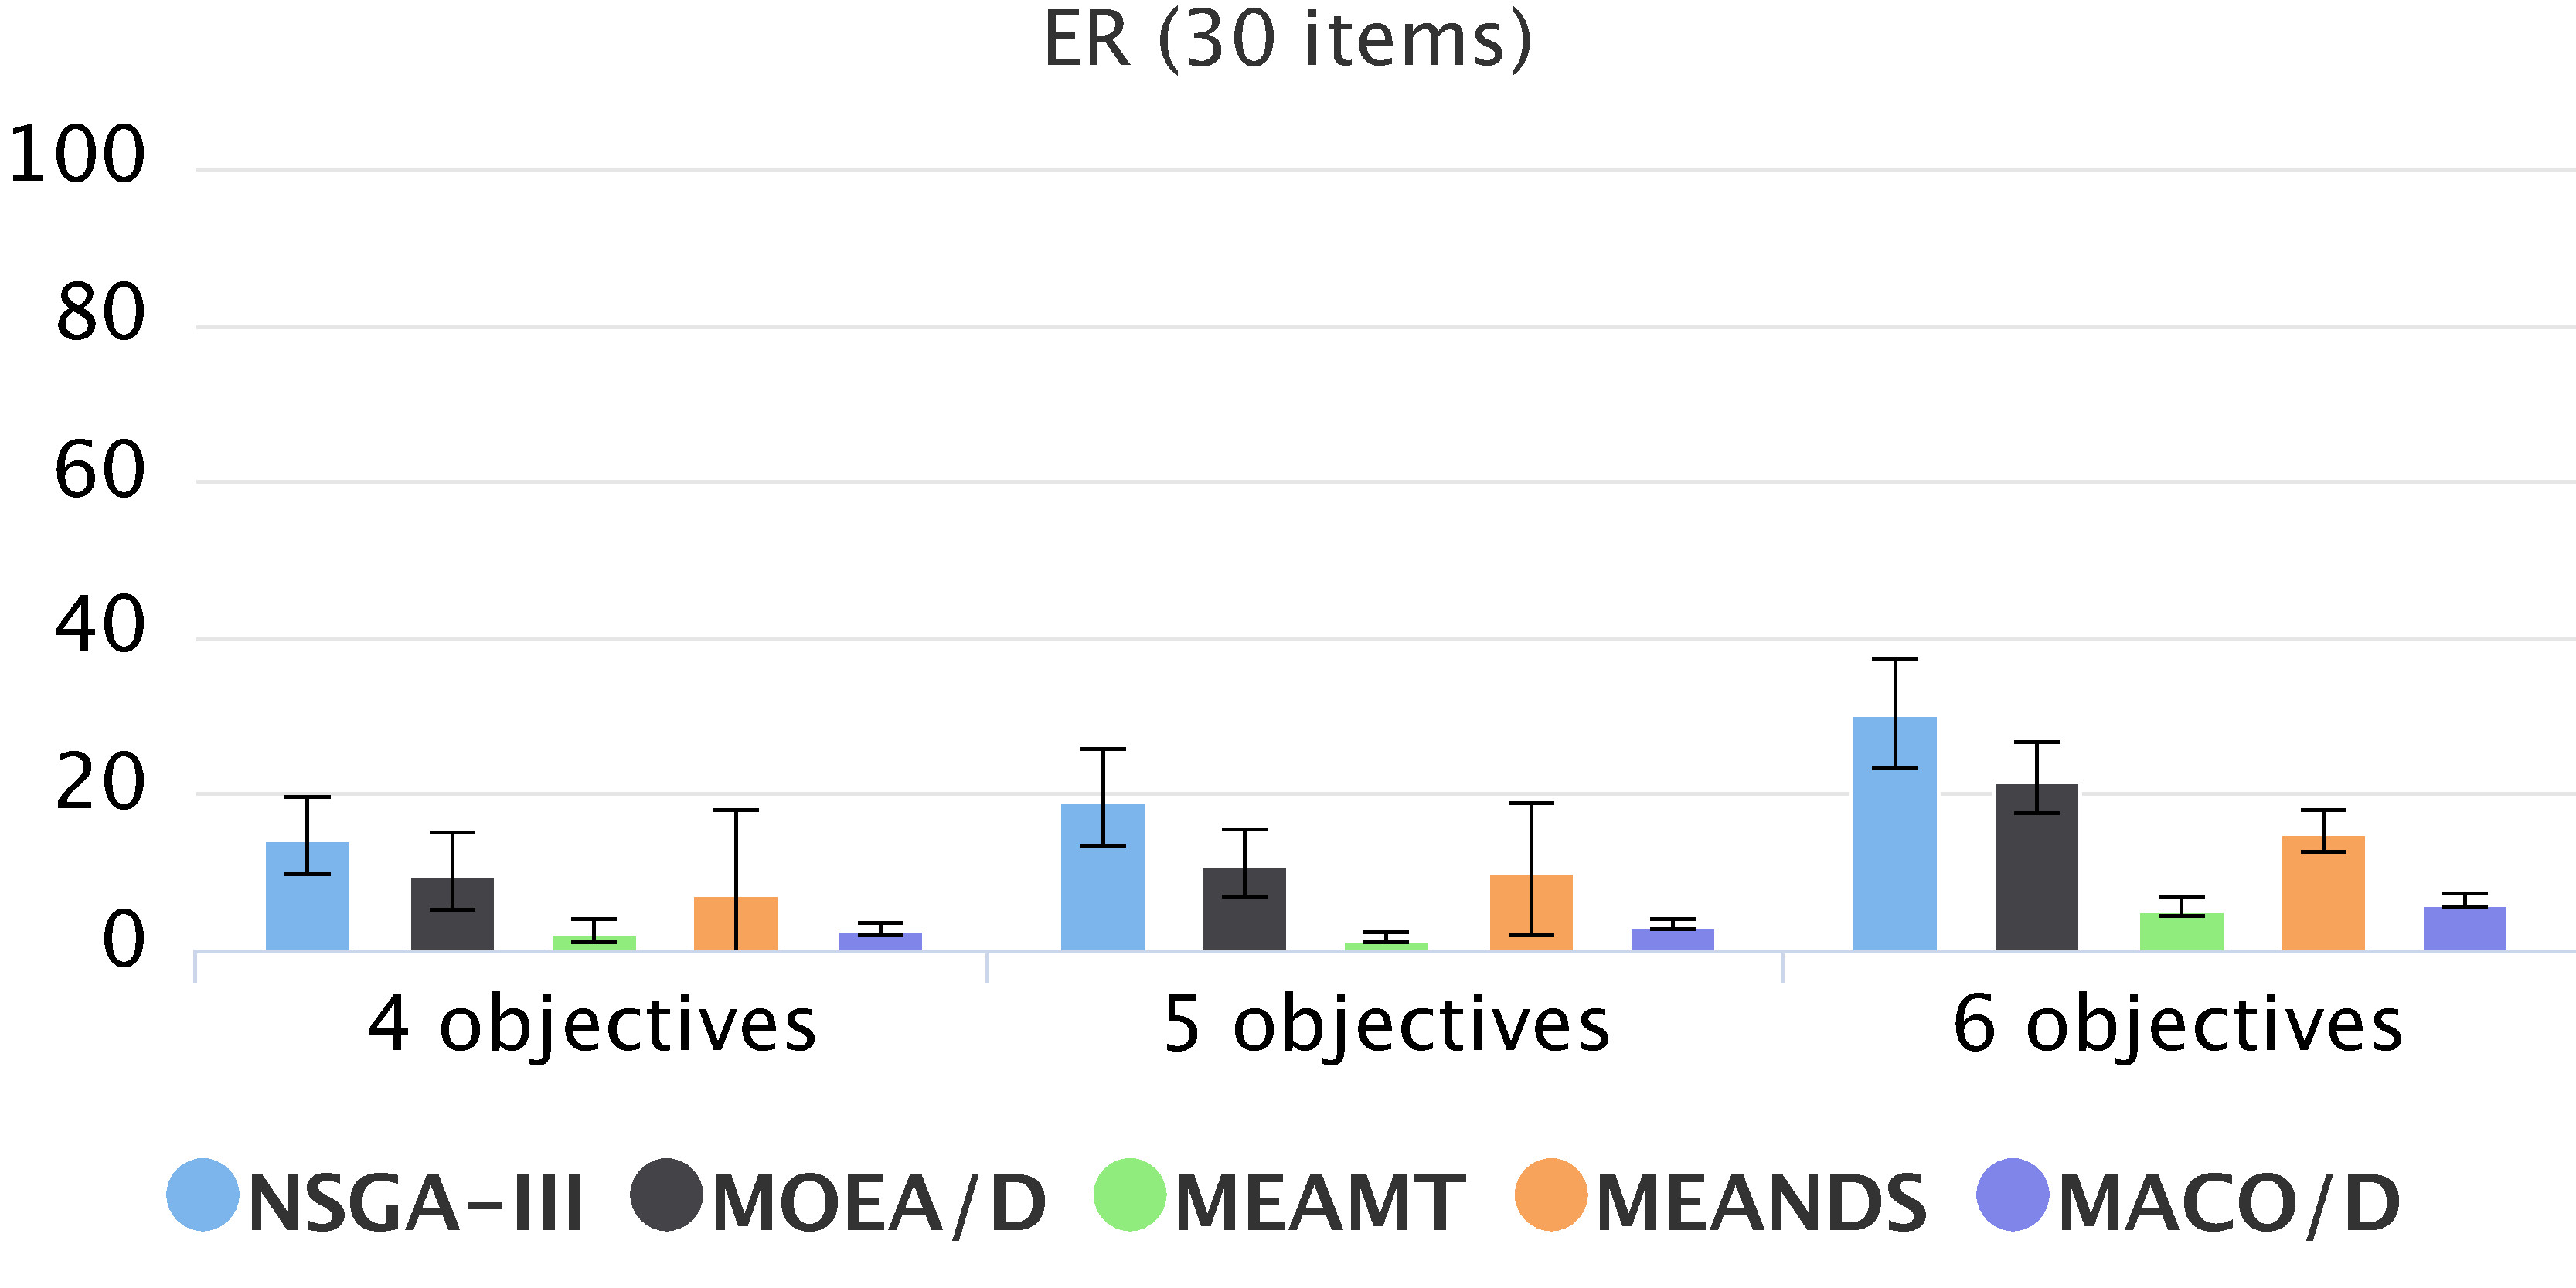
\includegraphics[width=0.5\textwidth]{cap_experimentos/figs/etapa2/er-mkp-30}
	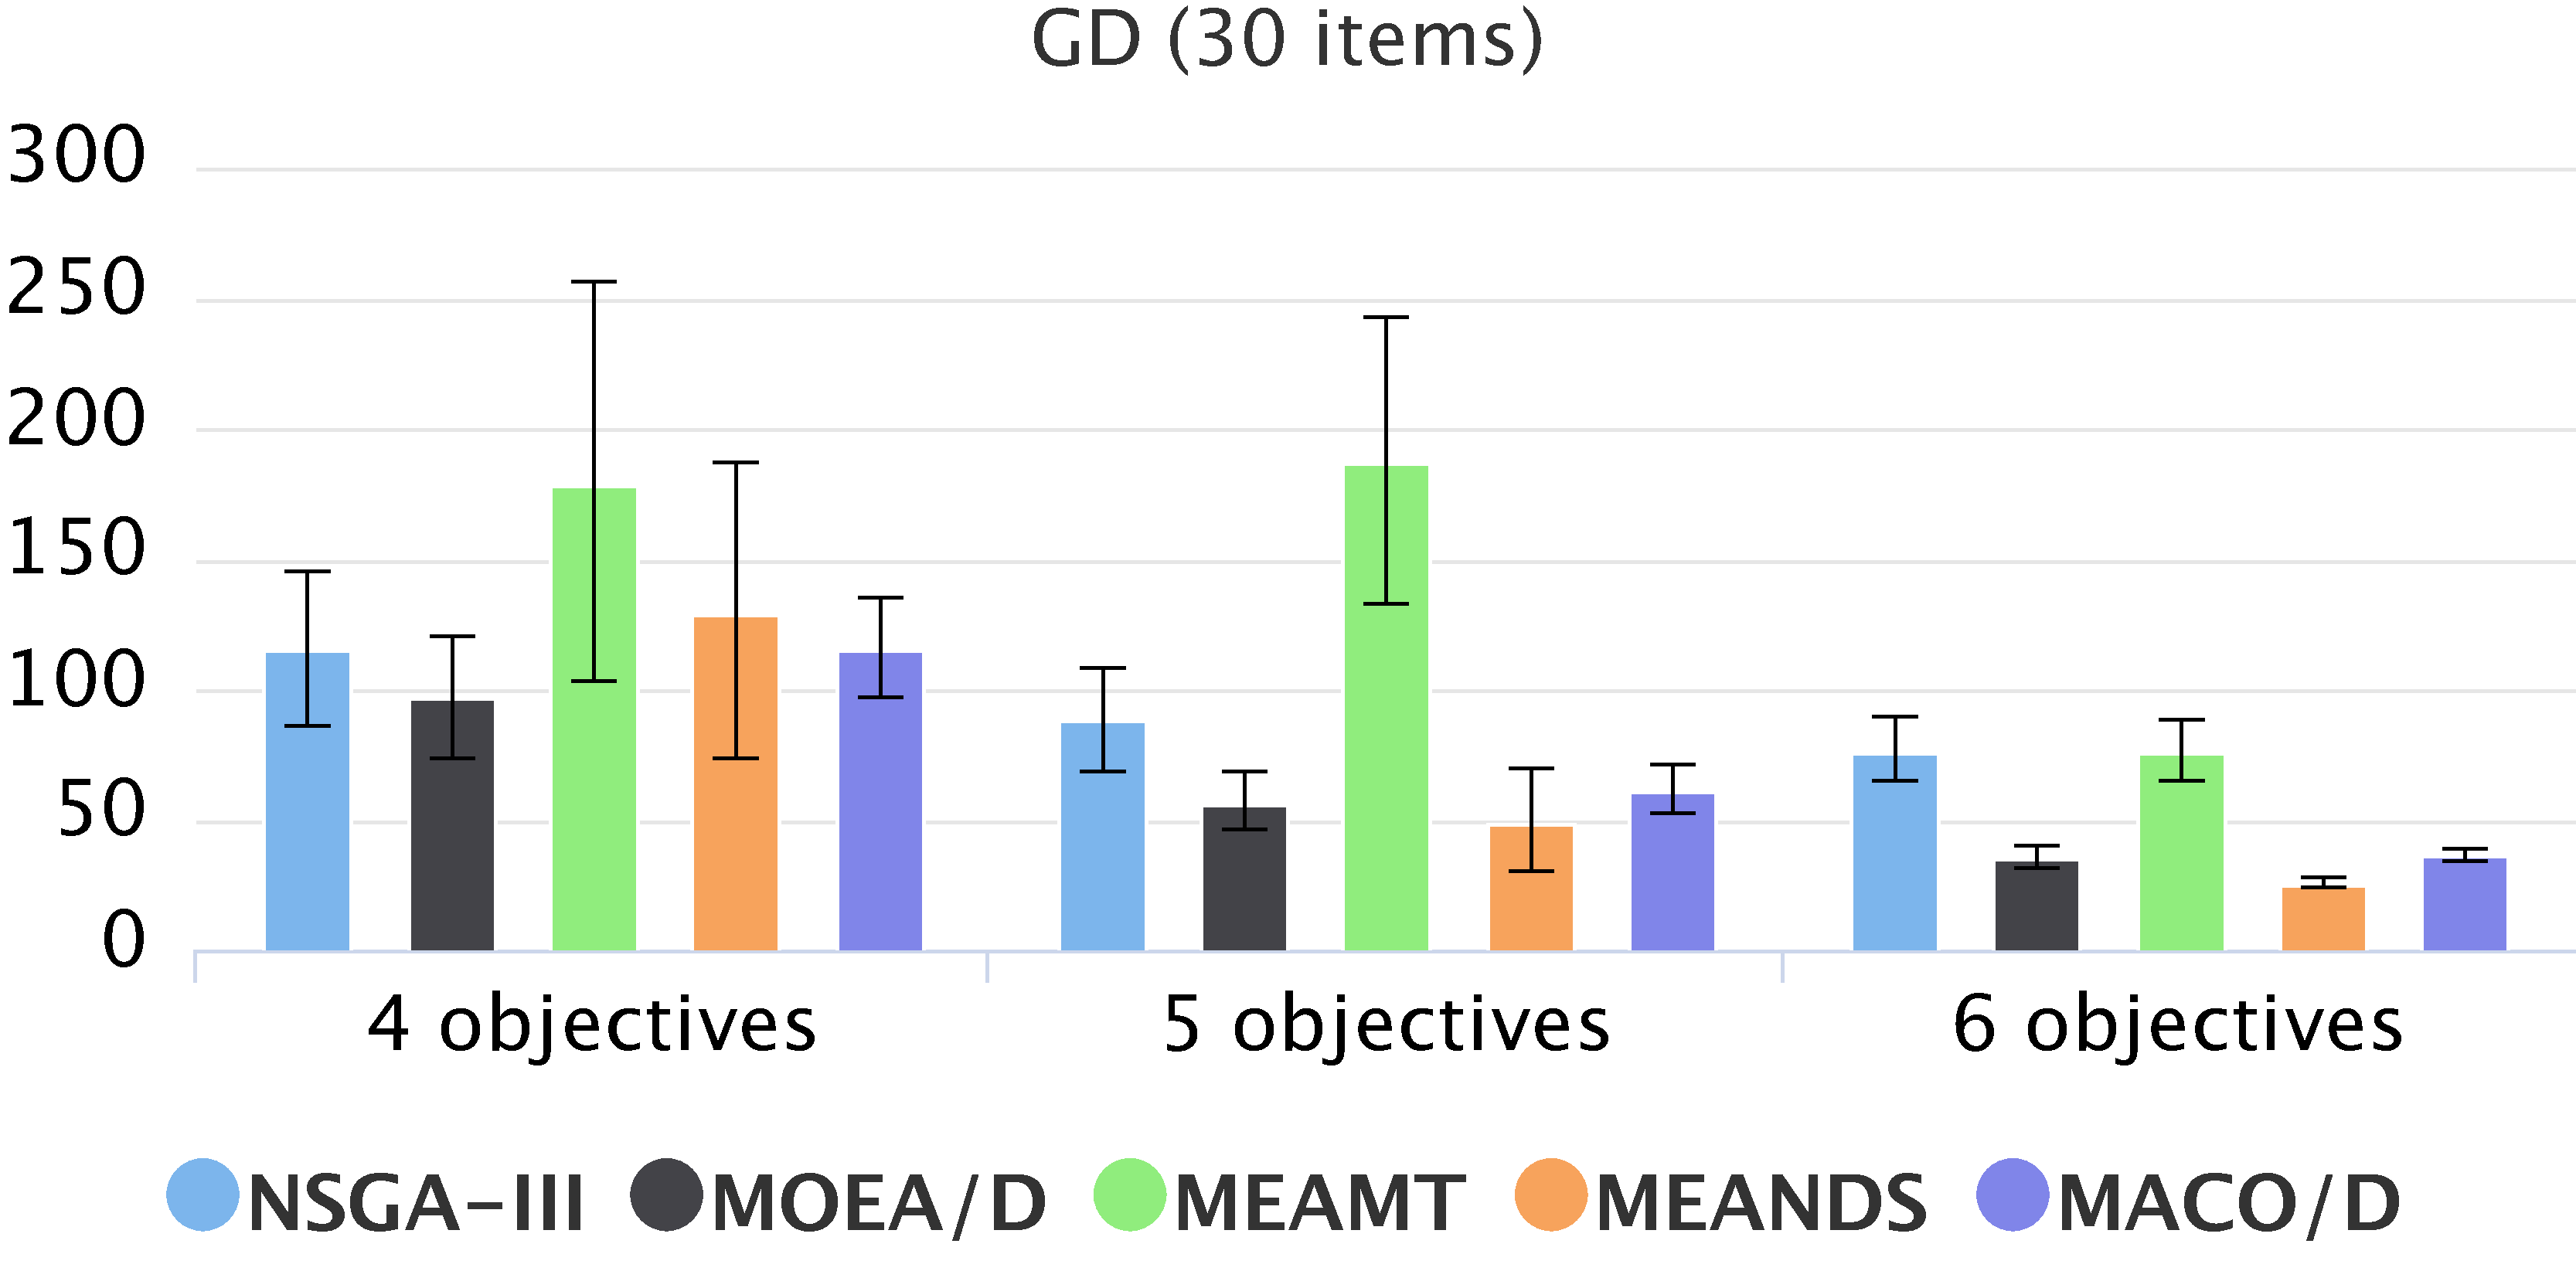
\includegraphics[width=0.5\textwidth]{cap_experimentos/figs/etapa2/gd-mkp-30}
	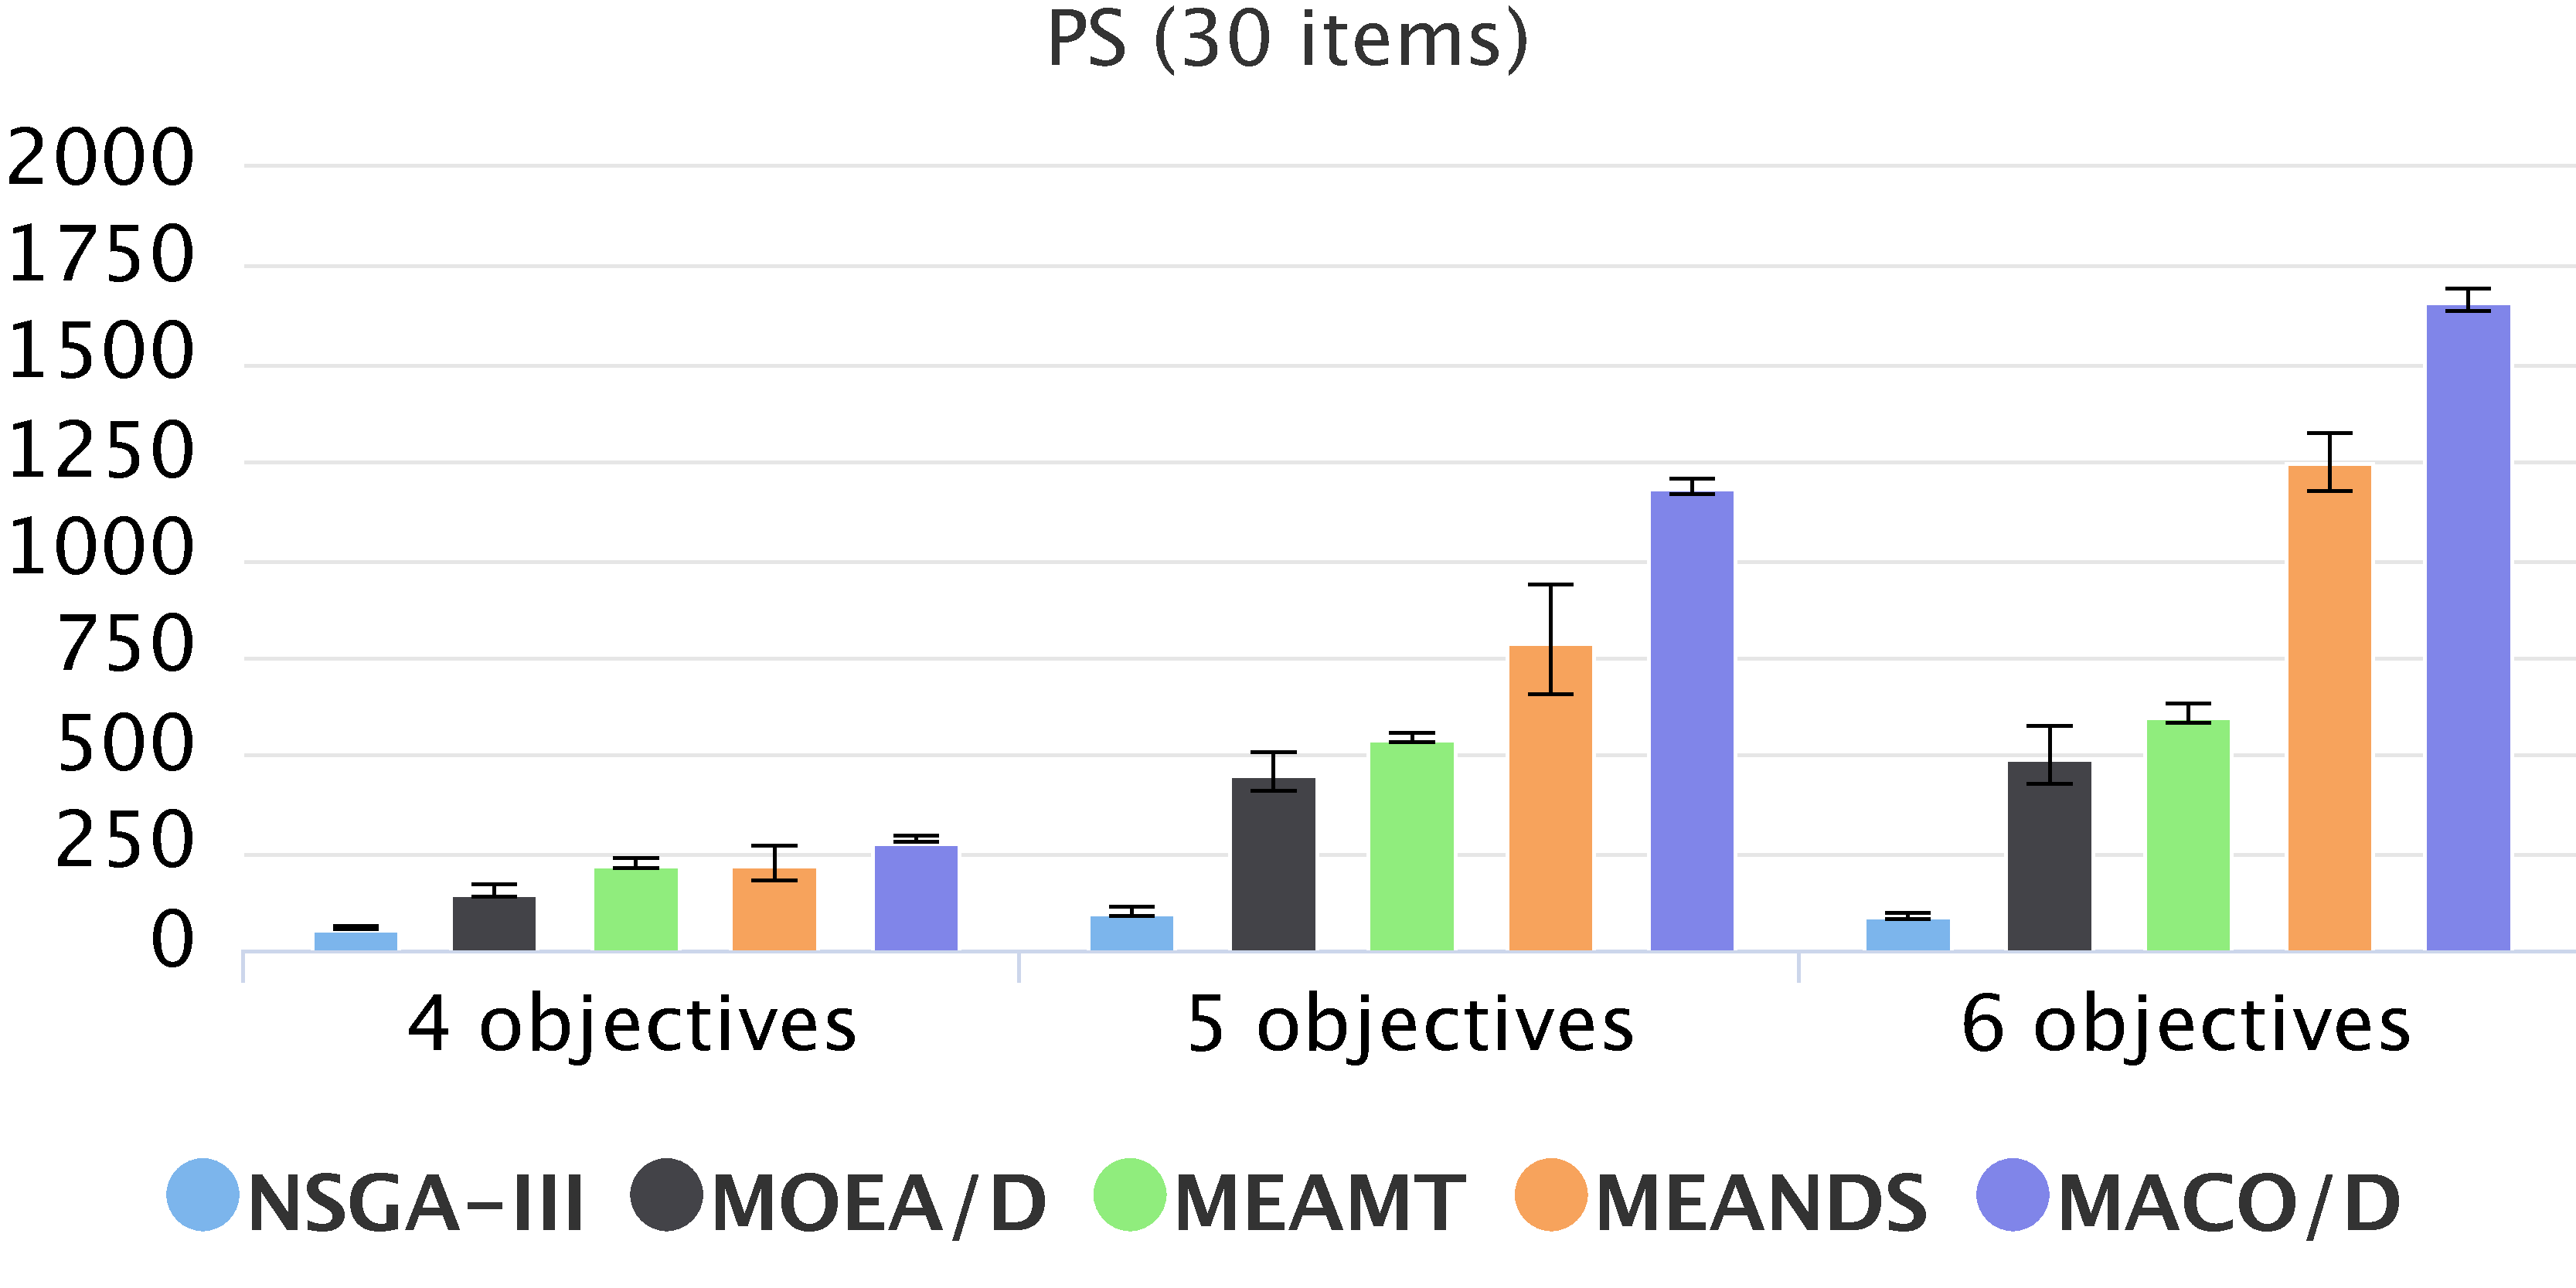
\includegraphics[width=0.5\textwidth]{cap_experimentos/figs/etapa2/ps-mkp-30}
	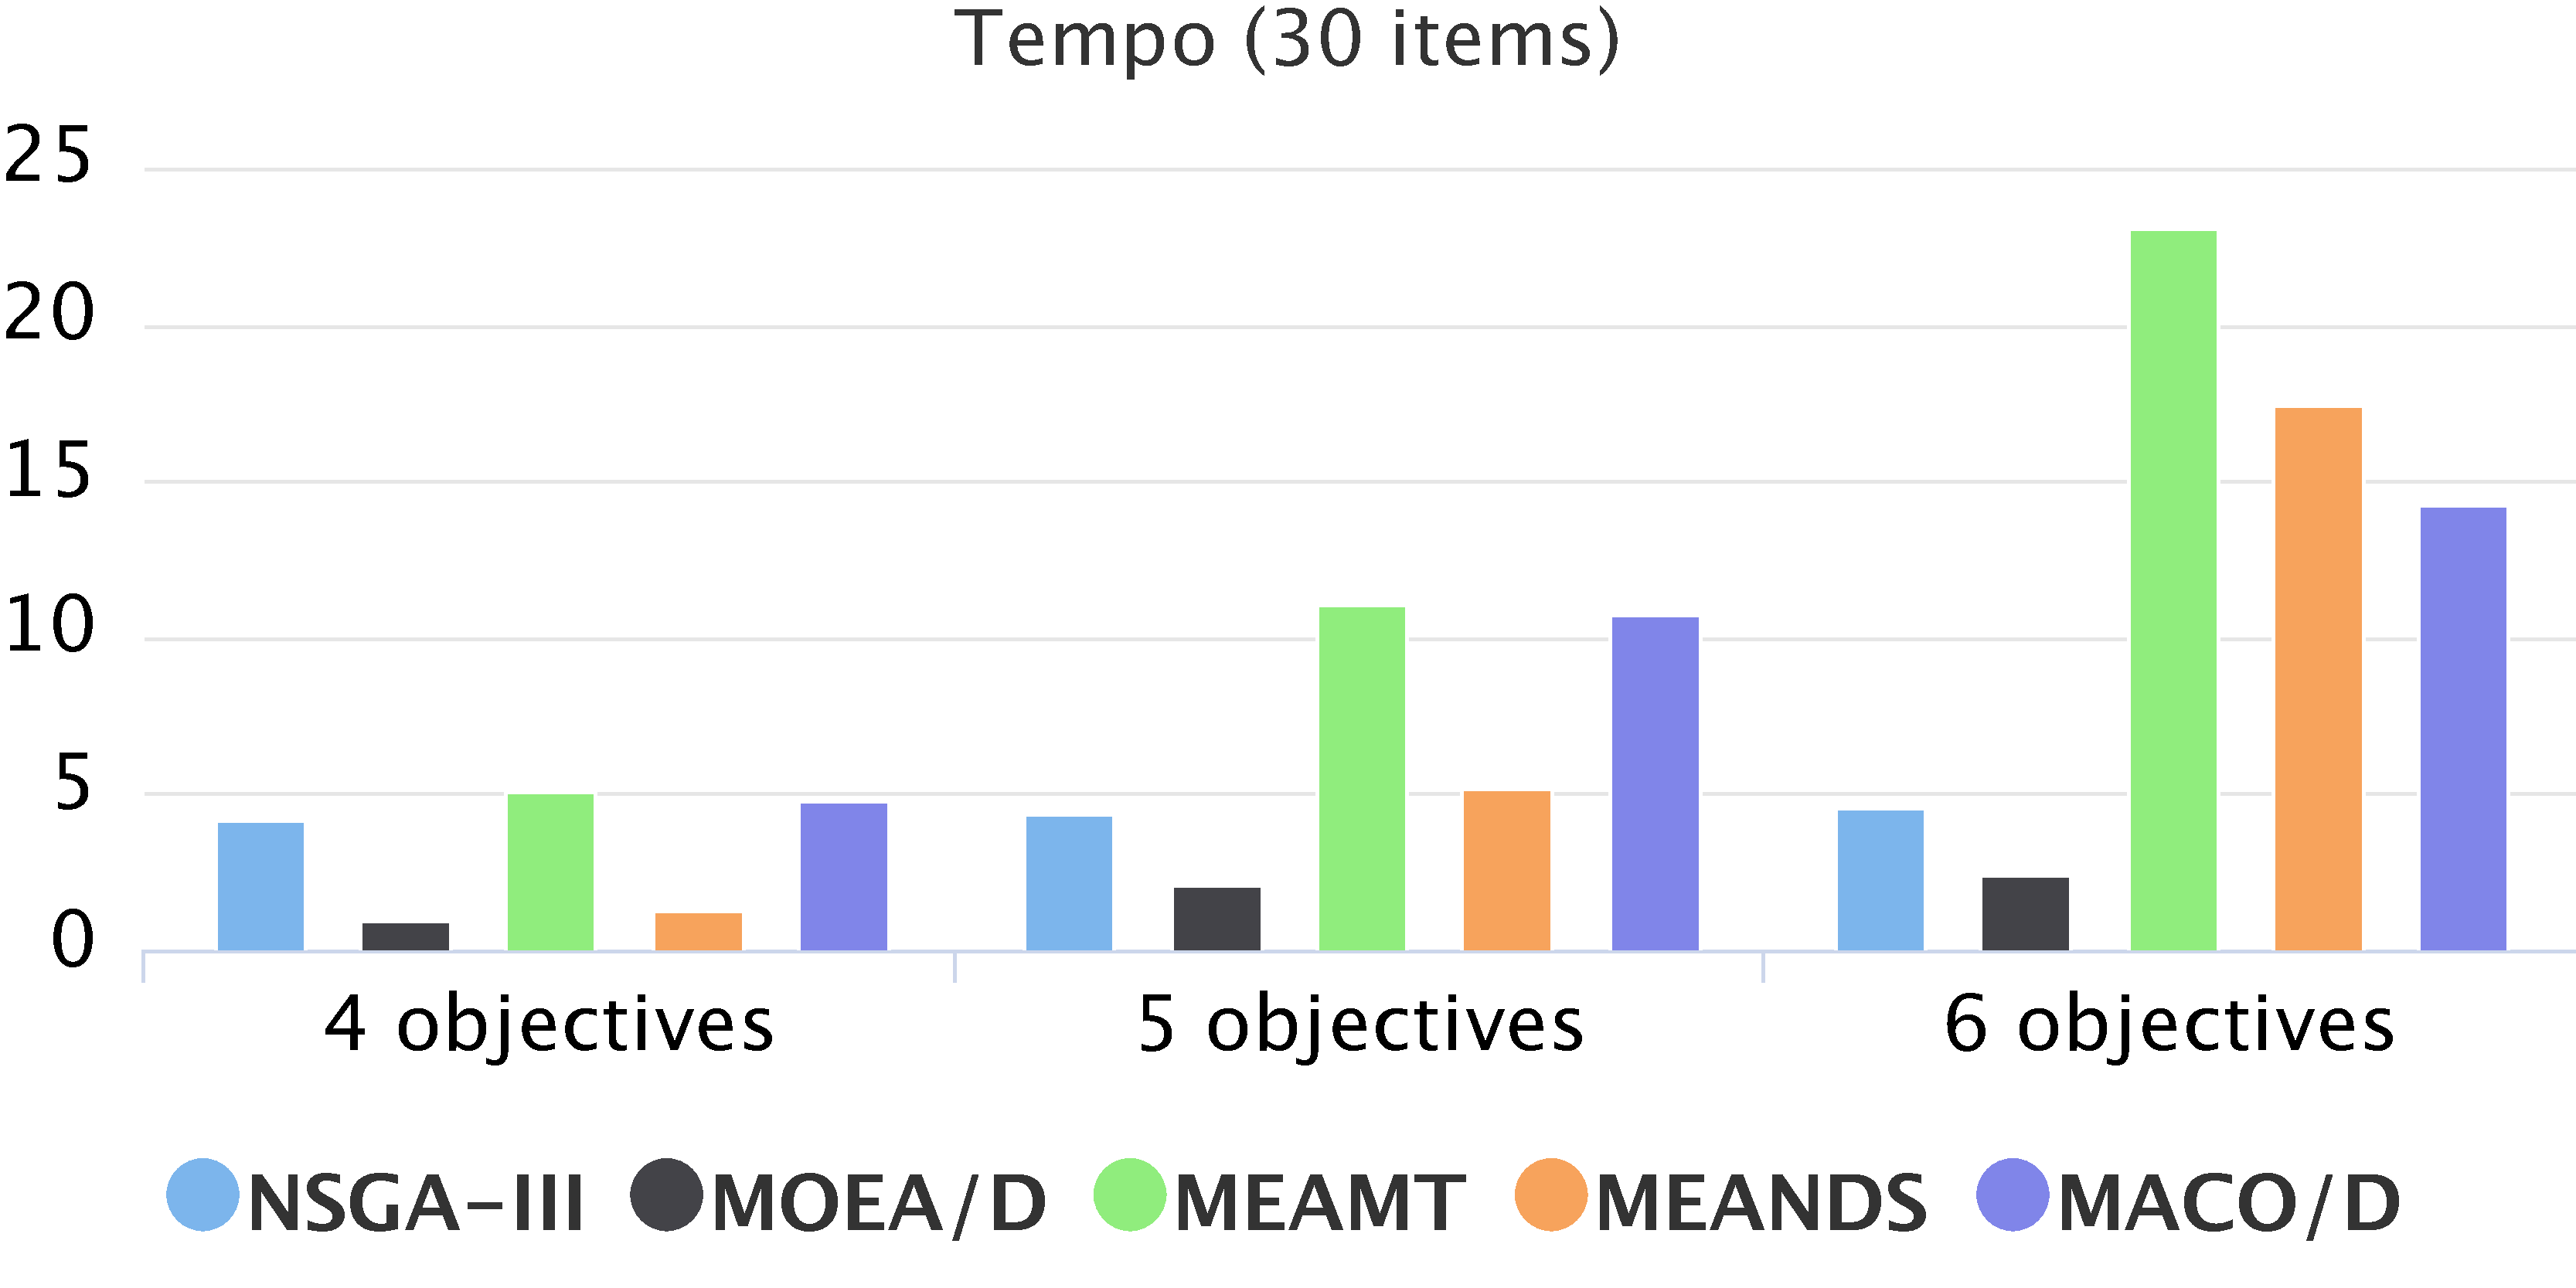
\includegraphics[width=0.5\textwidth]{cap_experimentos/figs/etapa2/time-mkp-30}
\end{figure*}

Análise do MKP-30

\begin{figure*}[!htbp]
	\caption{Etapa 2: resultados para o PMM com 50 itens}
	\label{fig_exp2_mkp_50}
	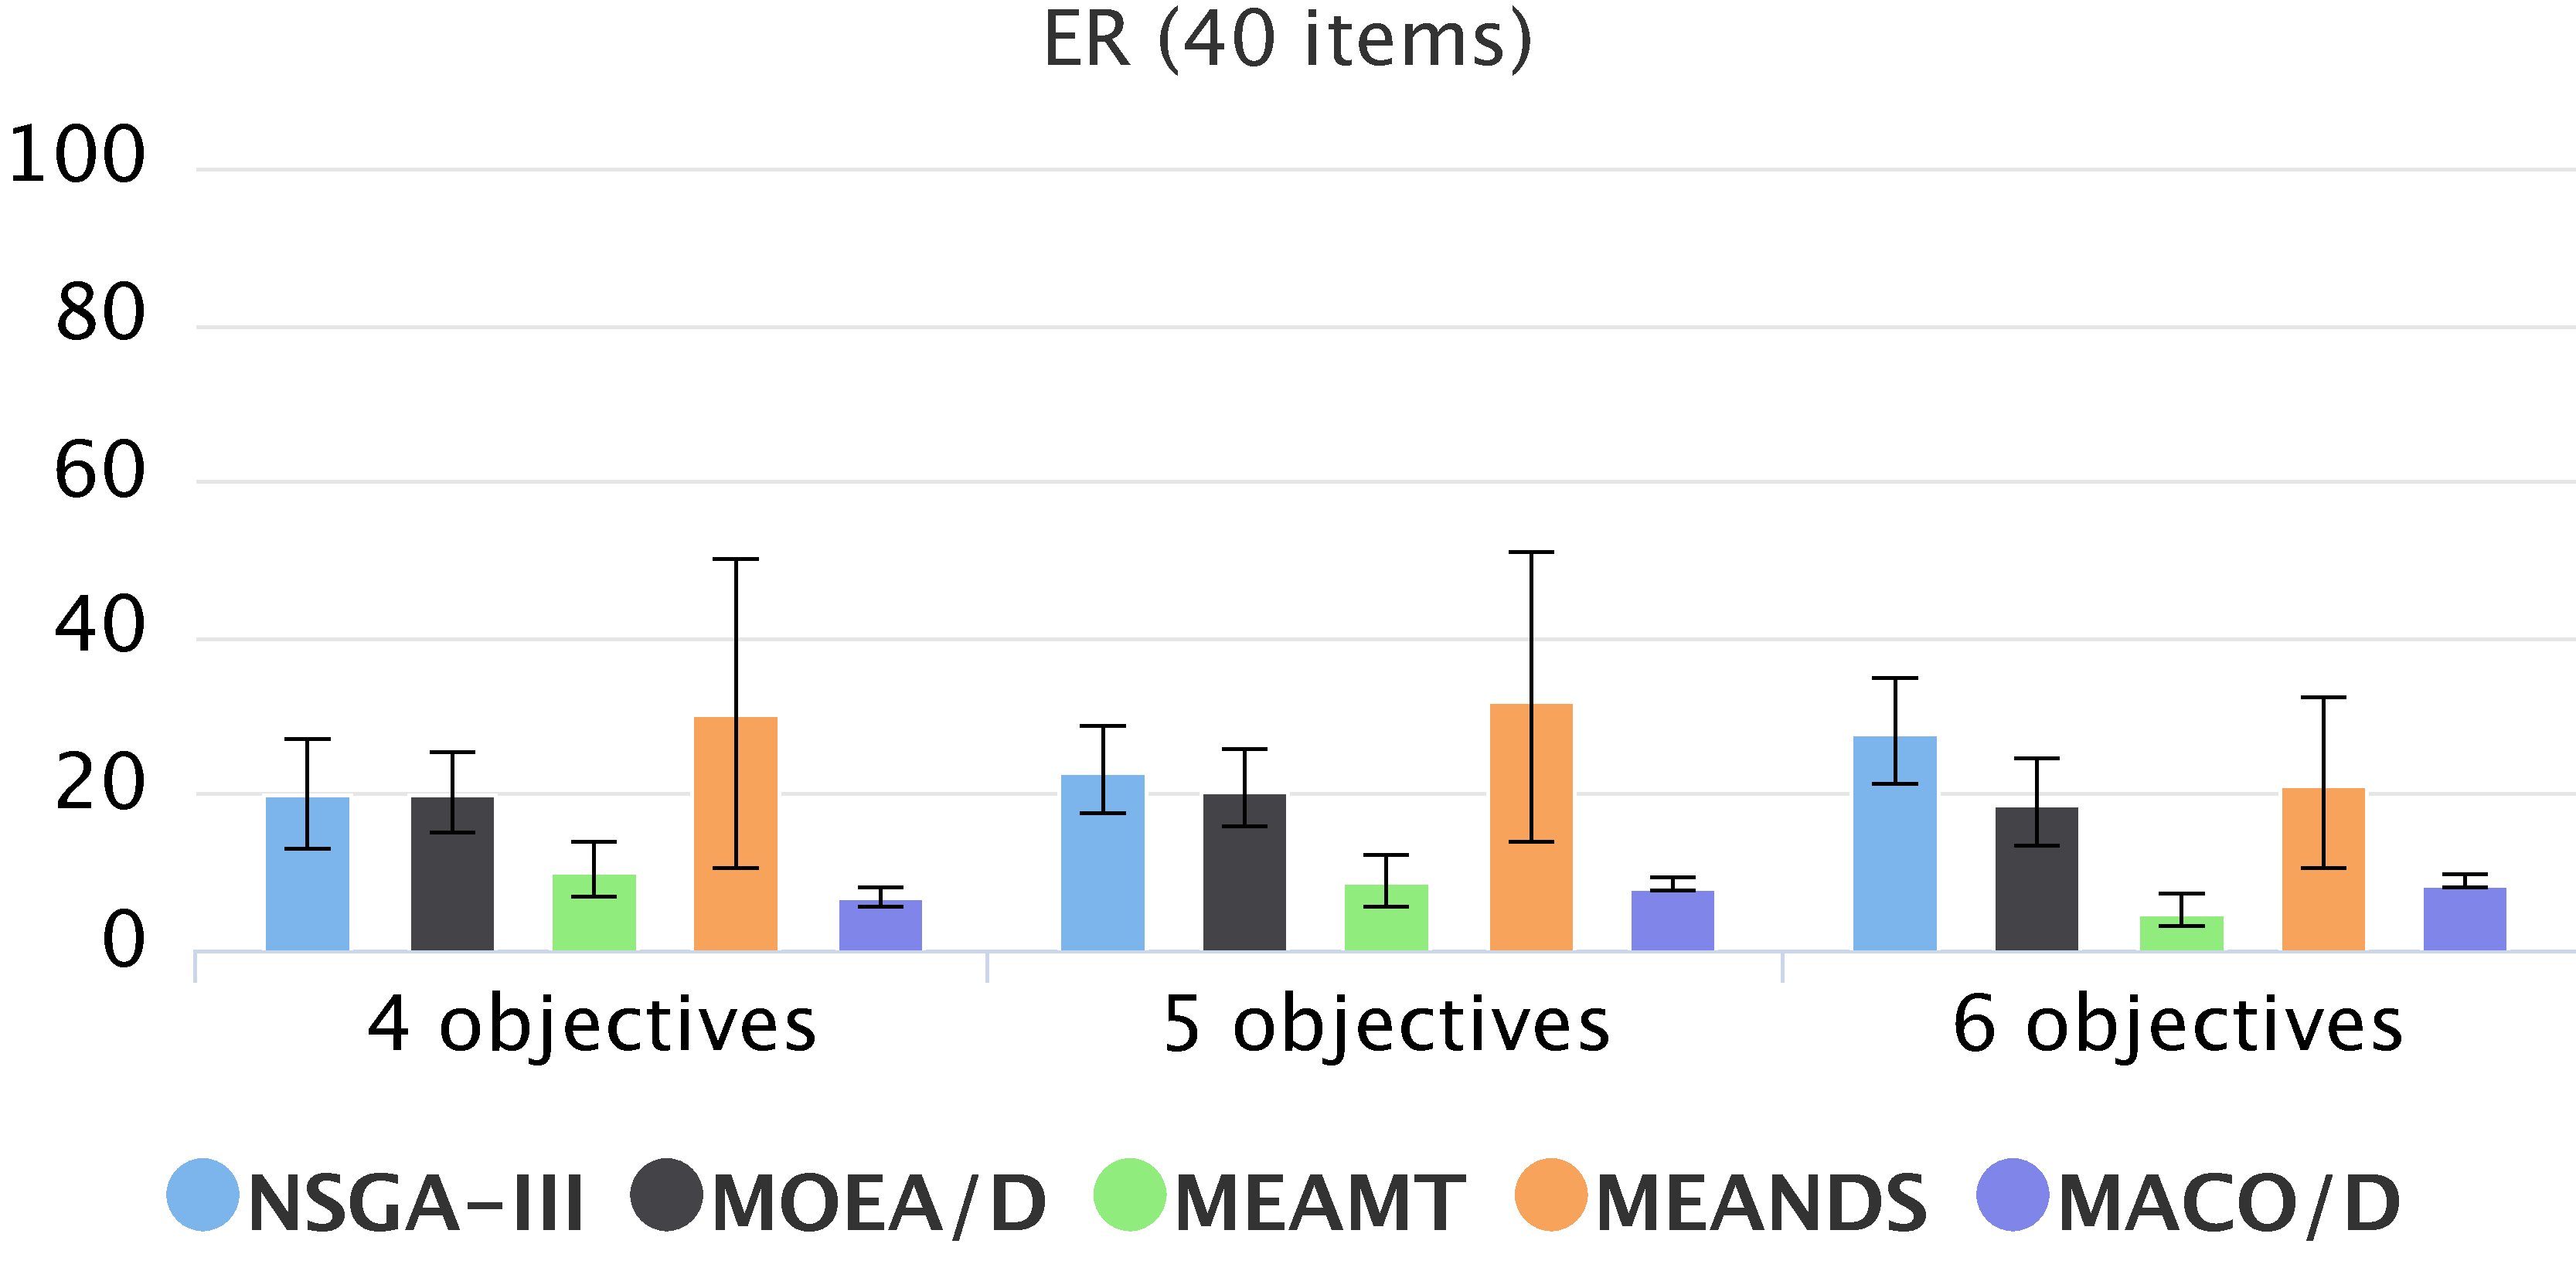
\includegraphics[width=0.5\textwidth]{cap_experimentos/figs/etapa2/er-mkp-40}
	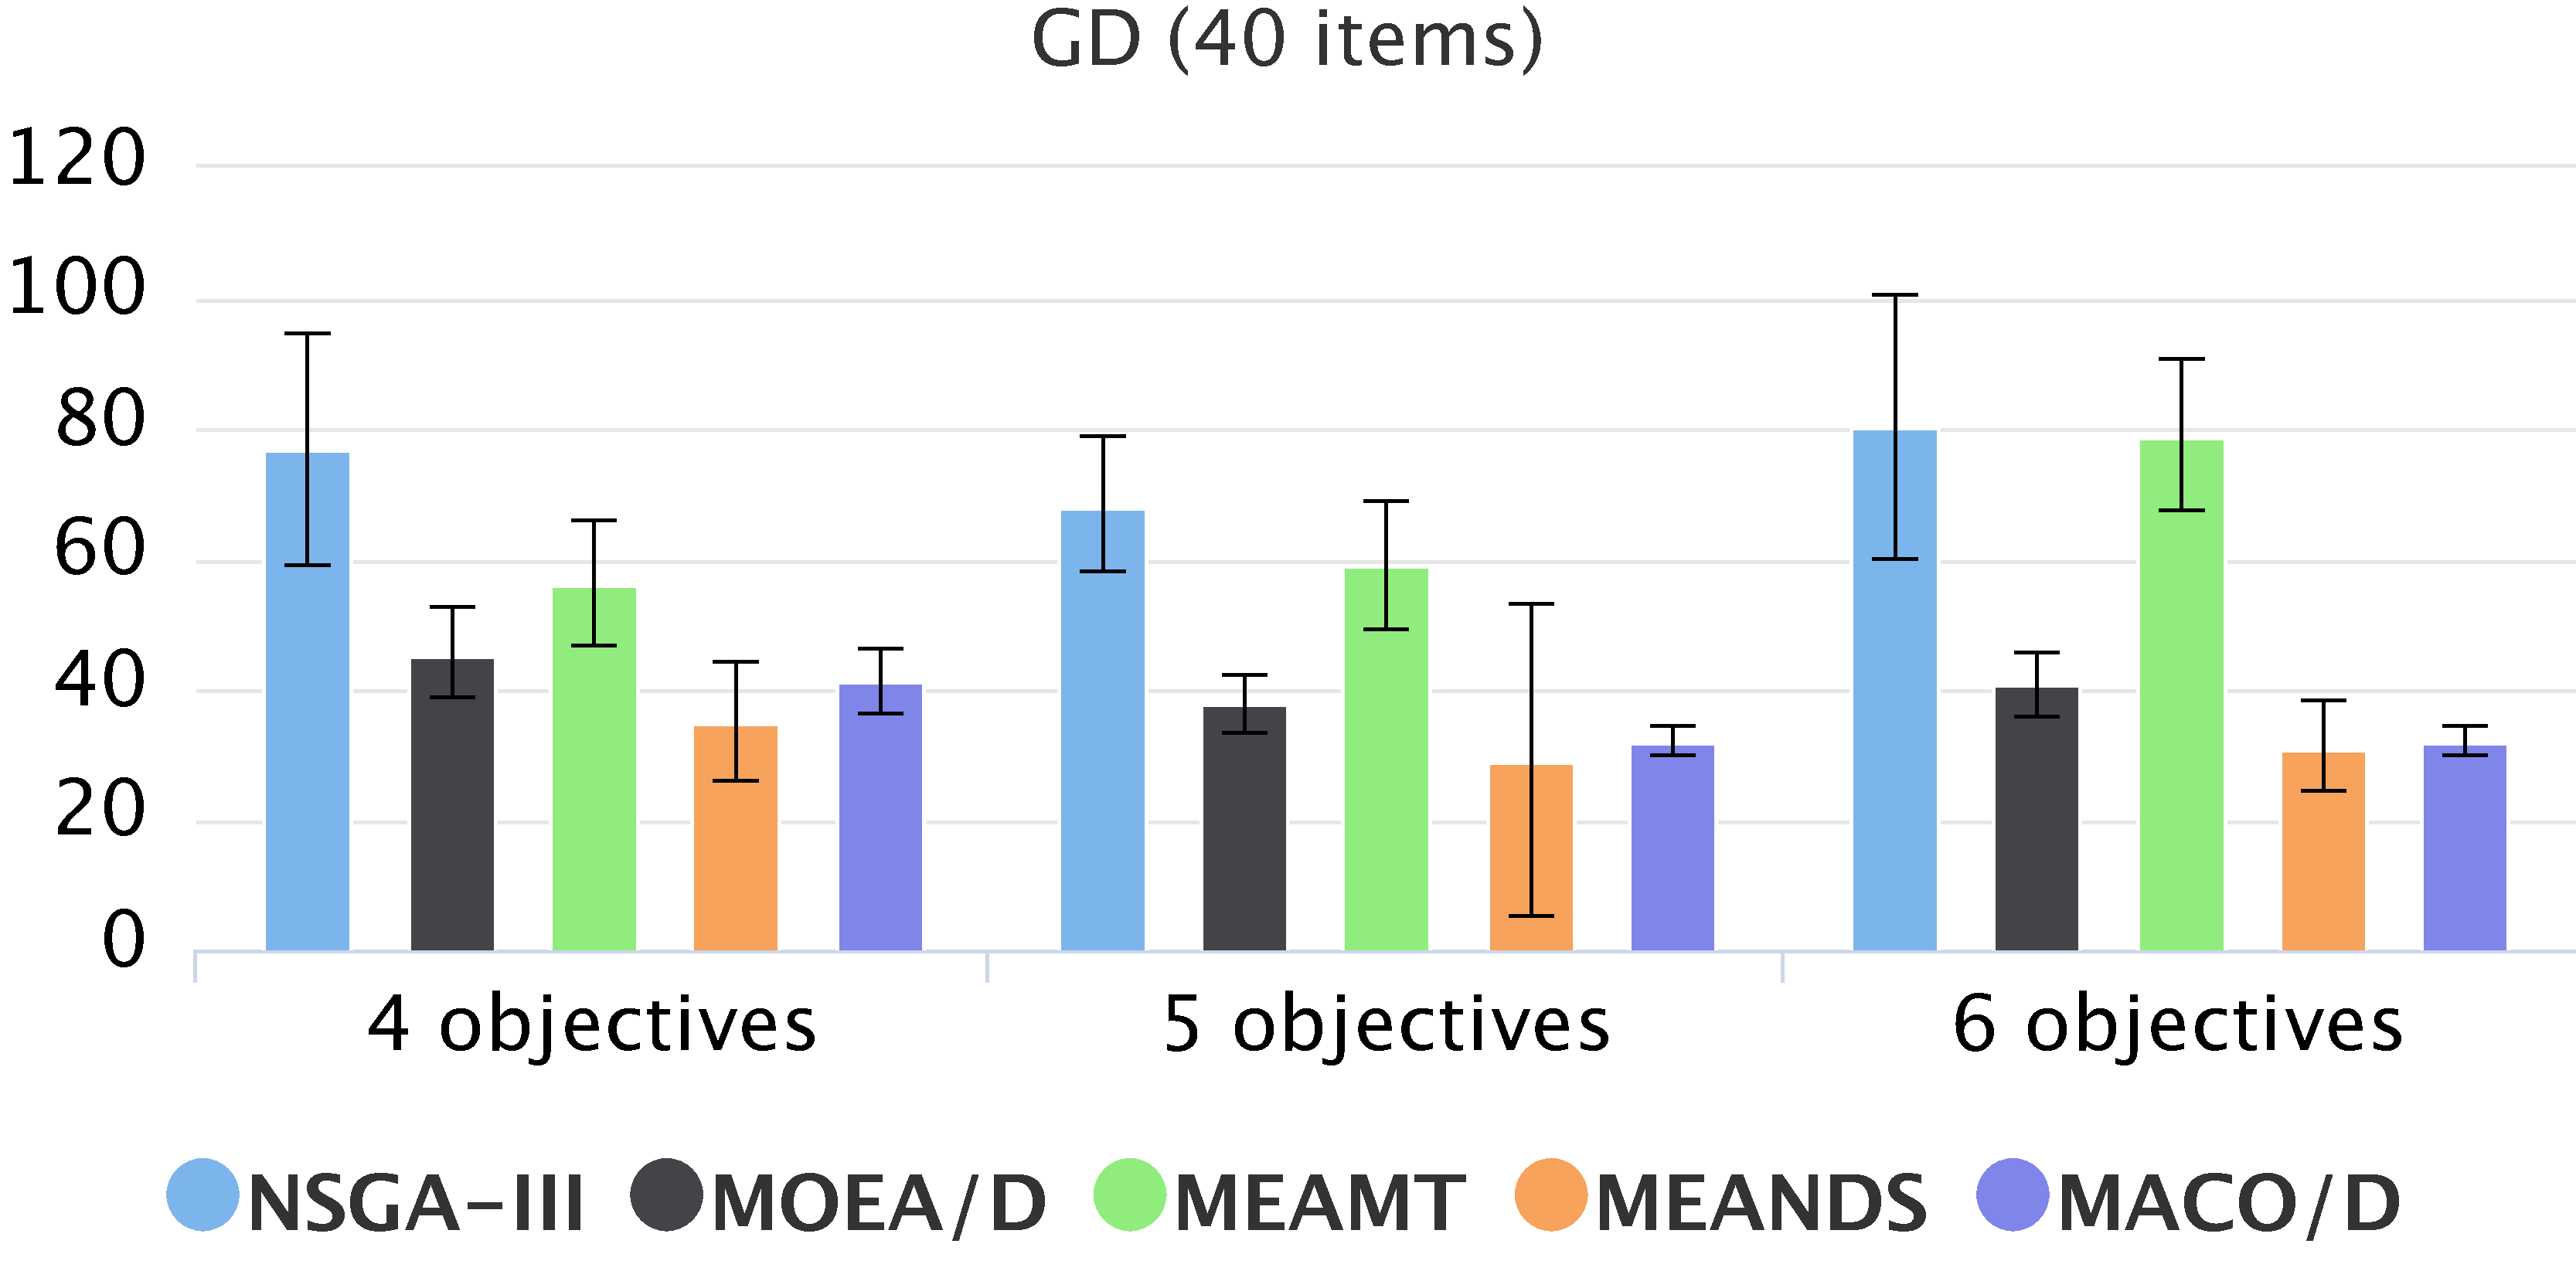
\includegraphics[width=0.5\textwidth]{cap_experimentos/figs/etapa2/gd-mkp-40}
	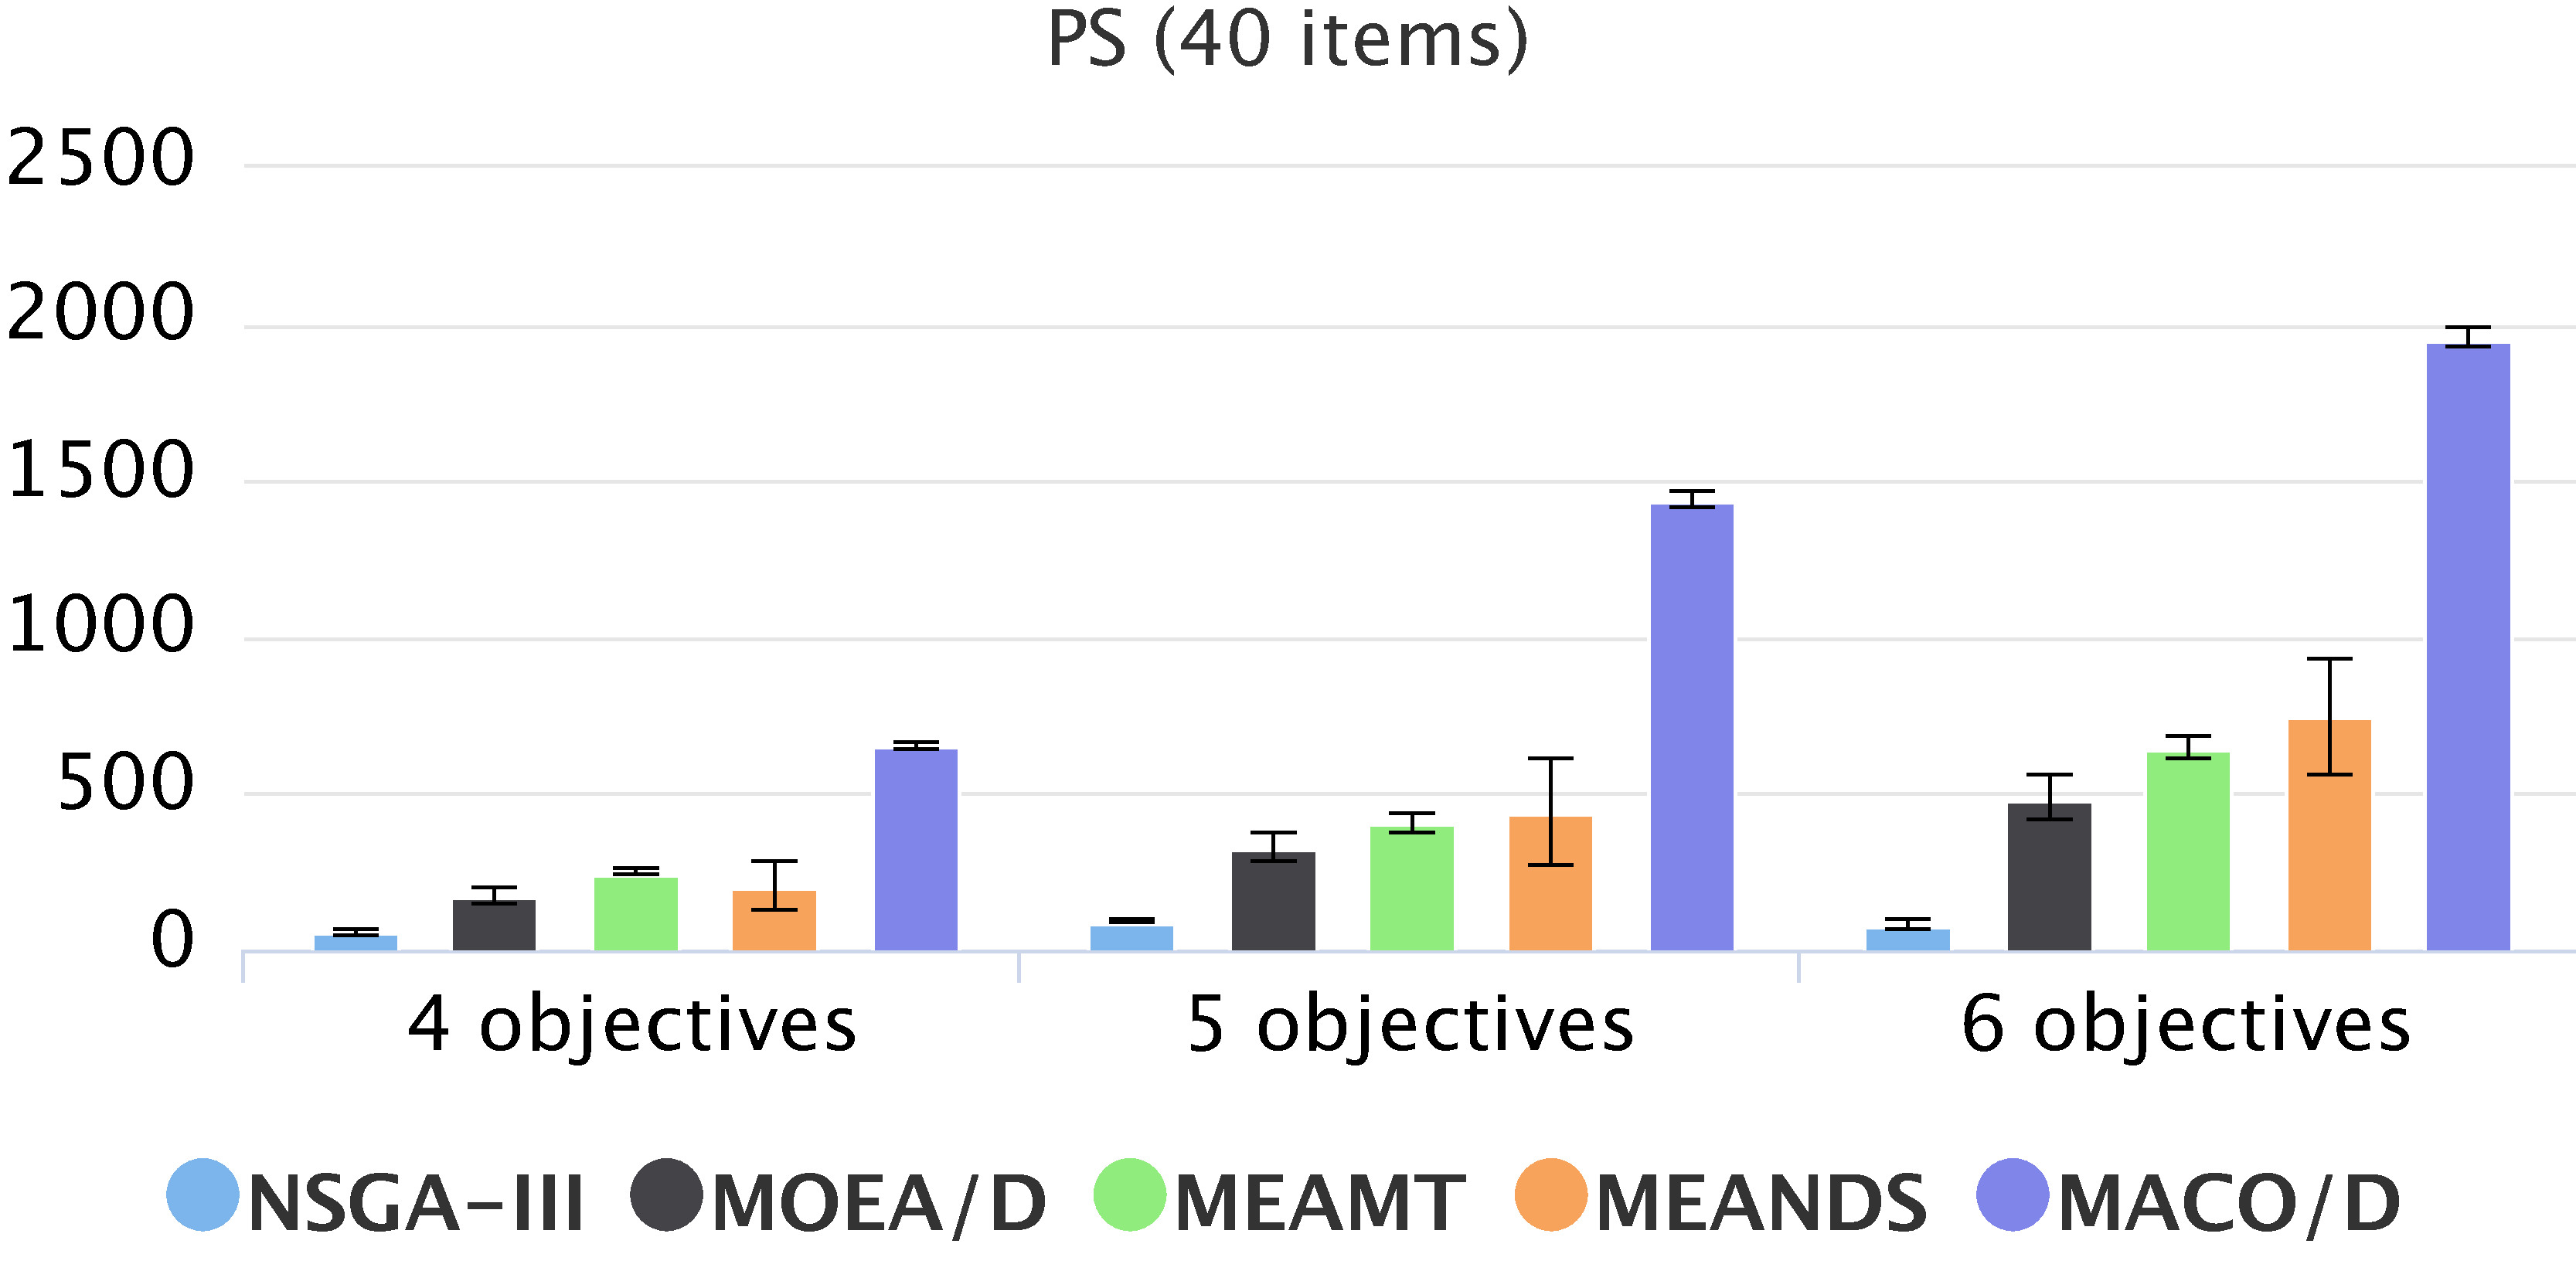
\includegraphics[width=0.5\textwidth]{cap_experimentos/figs/etapa2/ps-mkp-40}
	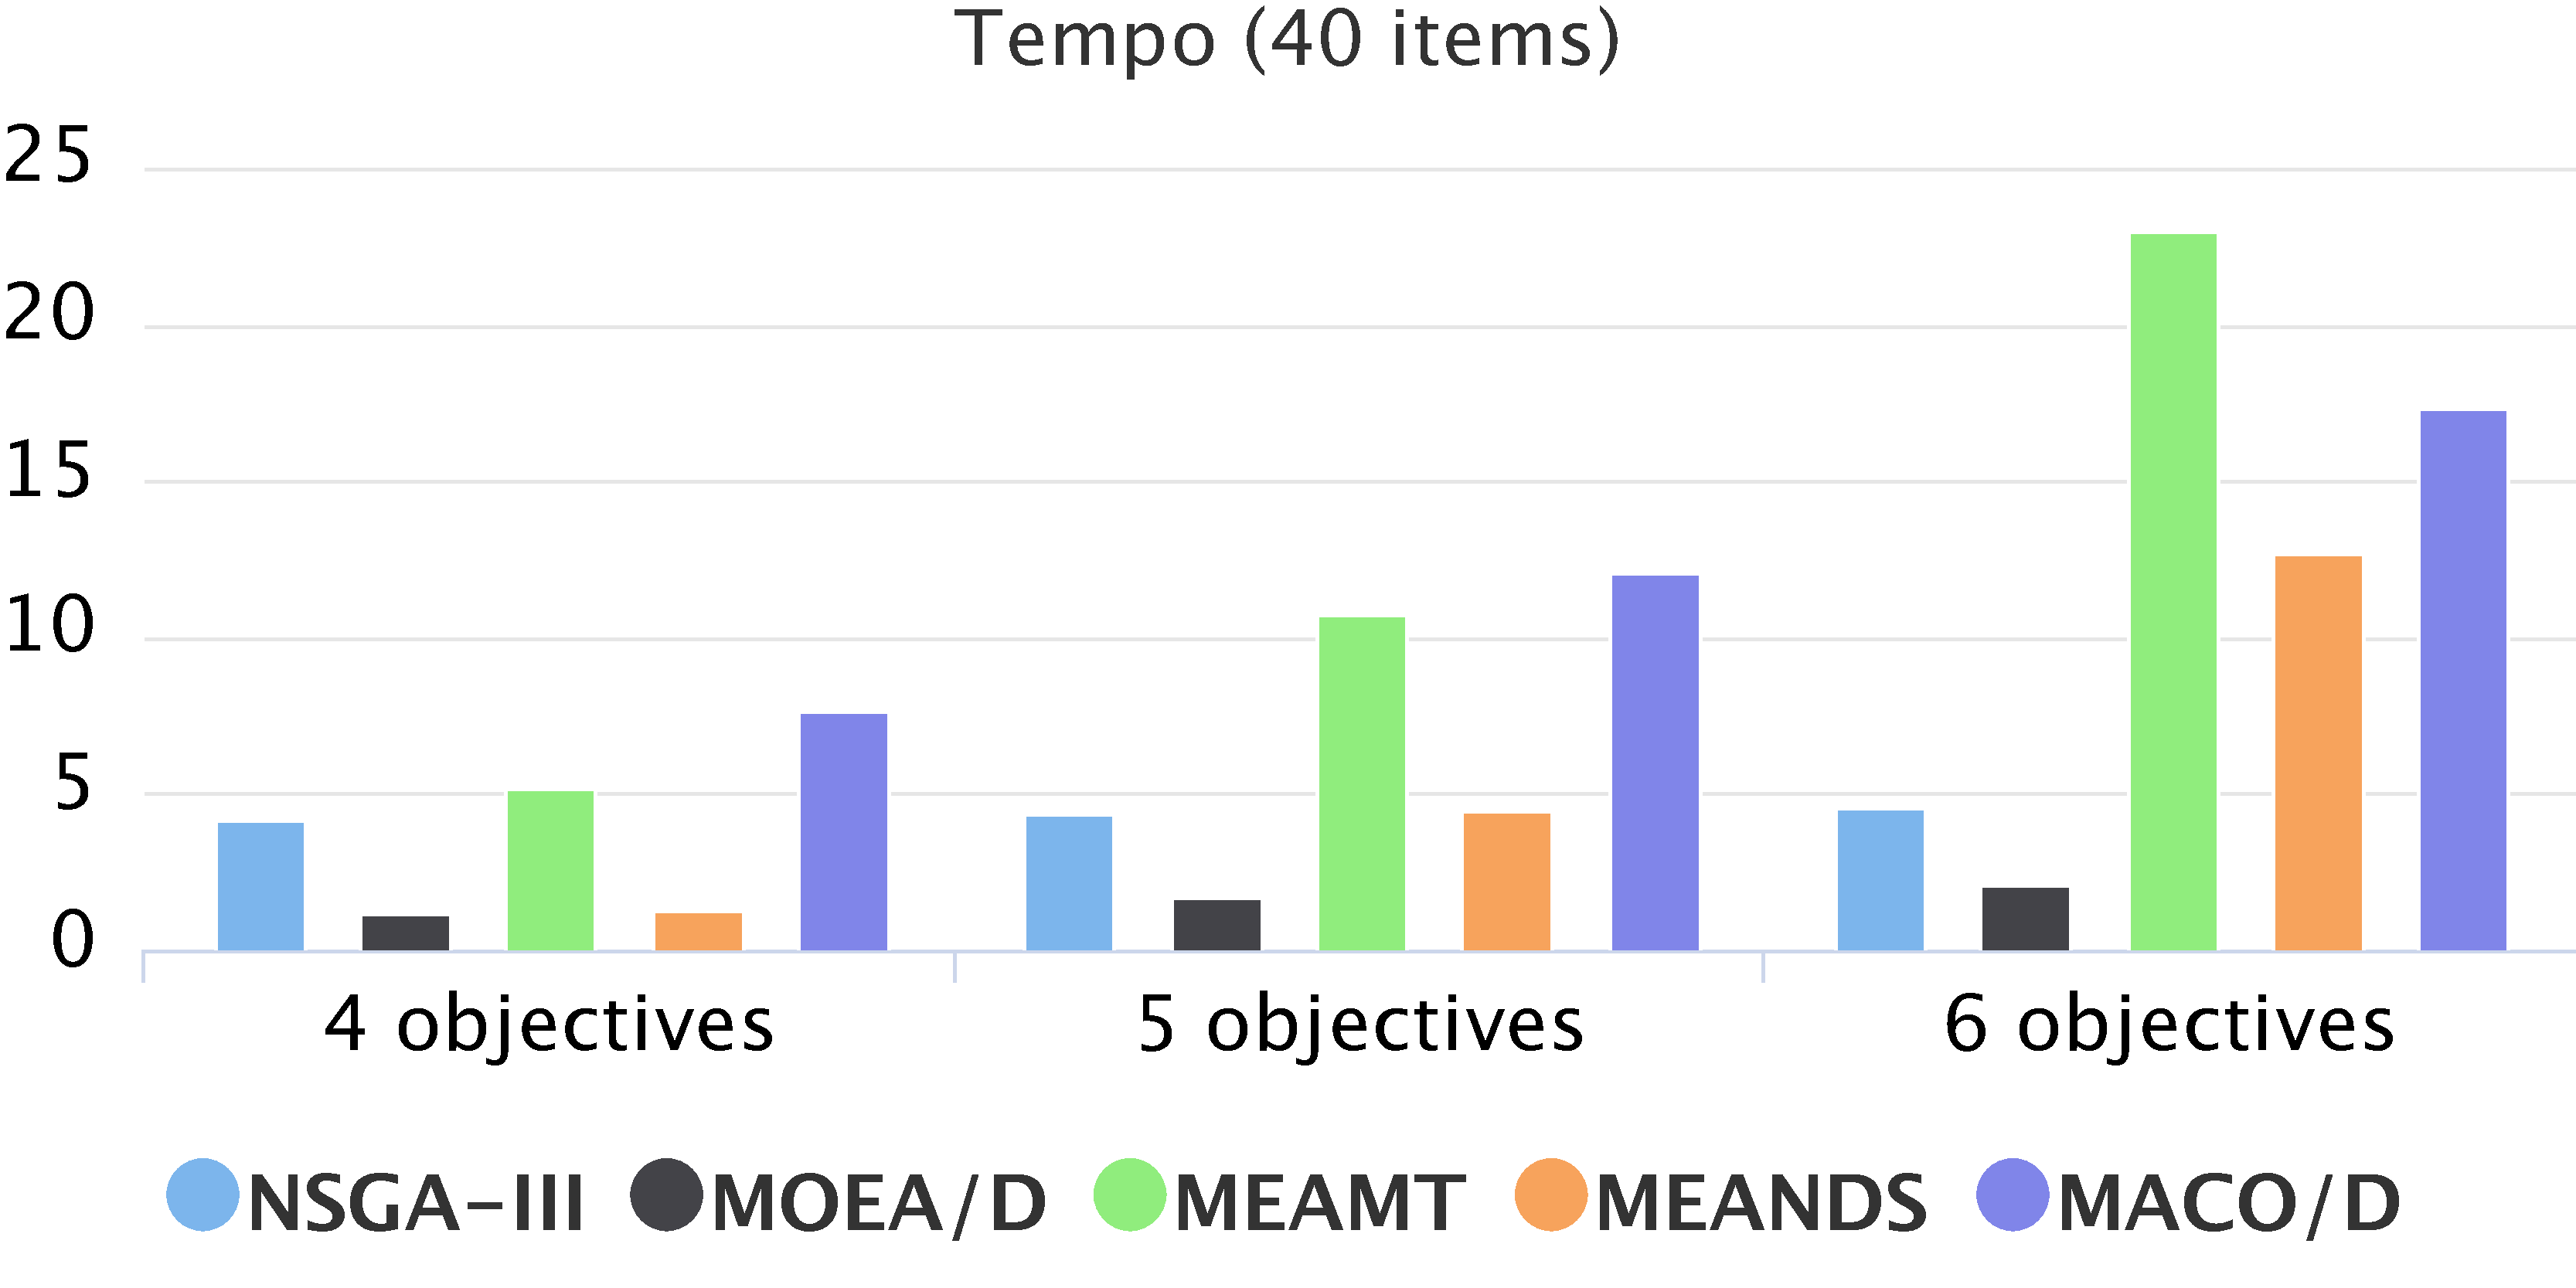
\includegraphics[width=0.5\textwidth]{cap_experimentos/figs/etapa2/time-mkp-40}
\end{figure*}

Análise do MKP-40

\begin{figure*}[!htbp]
	\caption{Etapa 2: resultados para o PMM com 100 itens}
	\label{fig_exp2_mkp_100}
	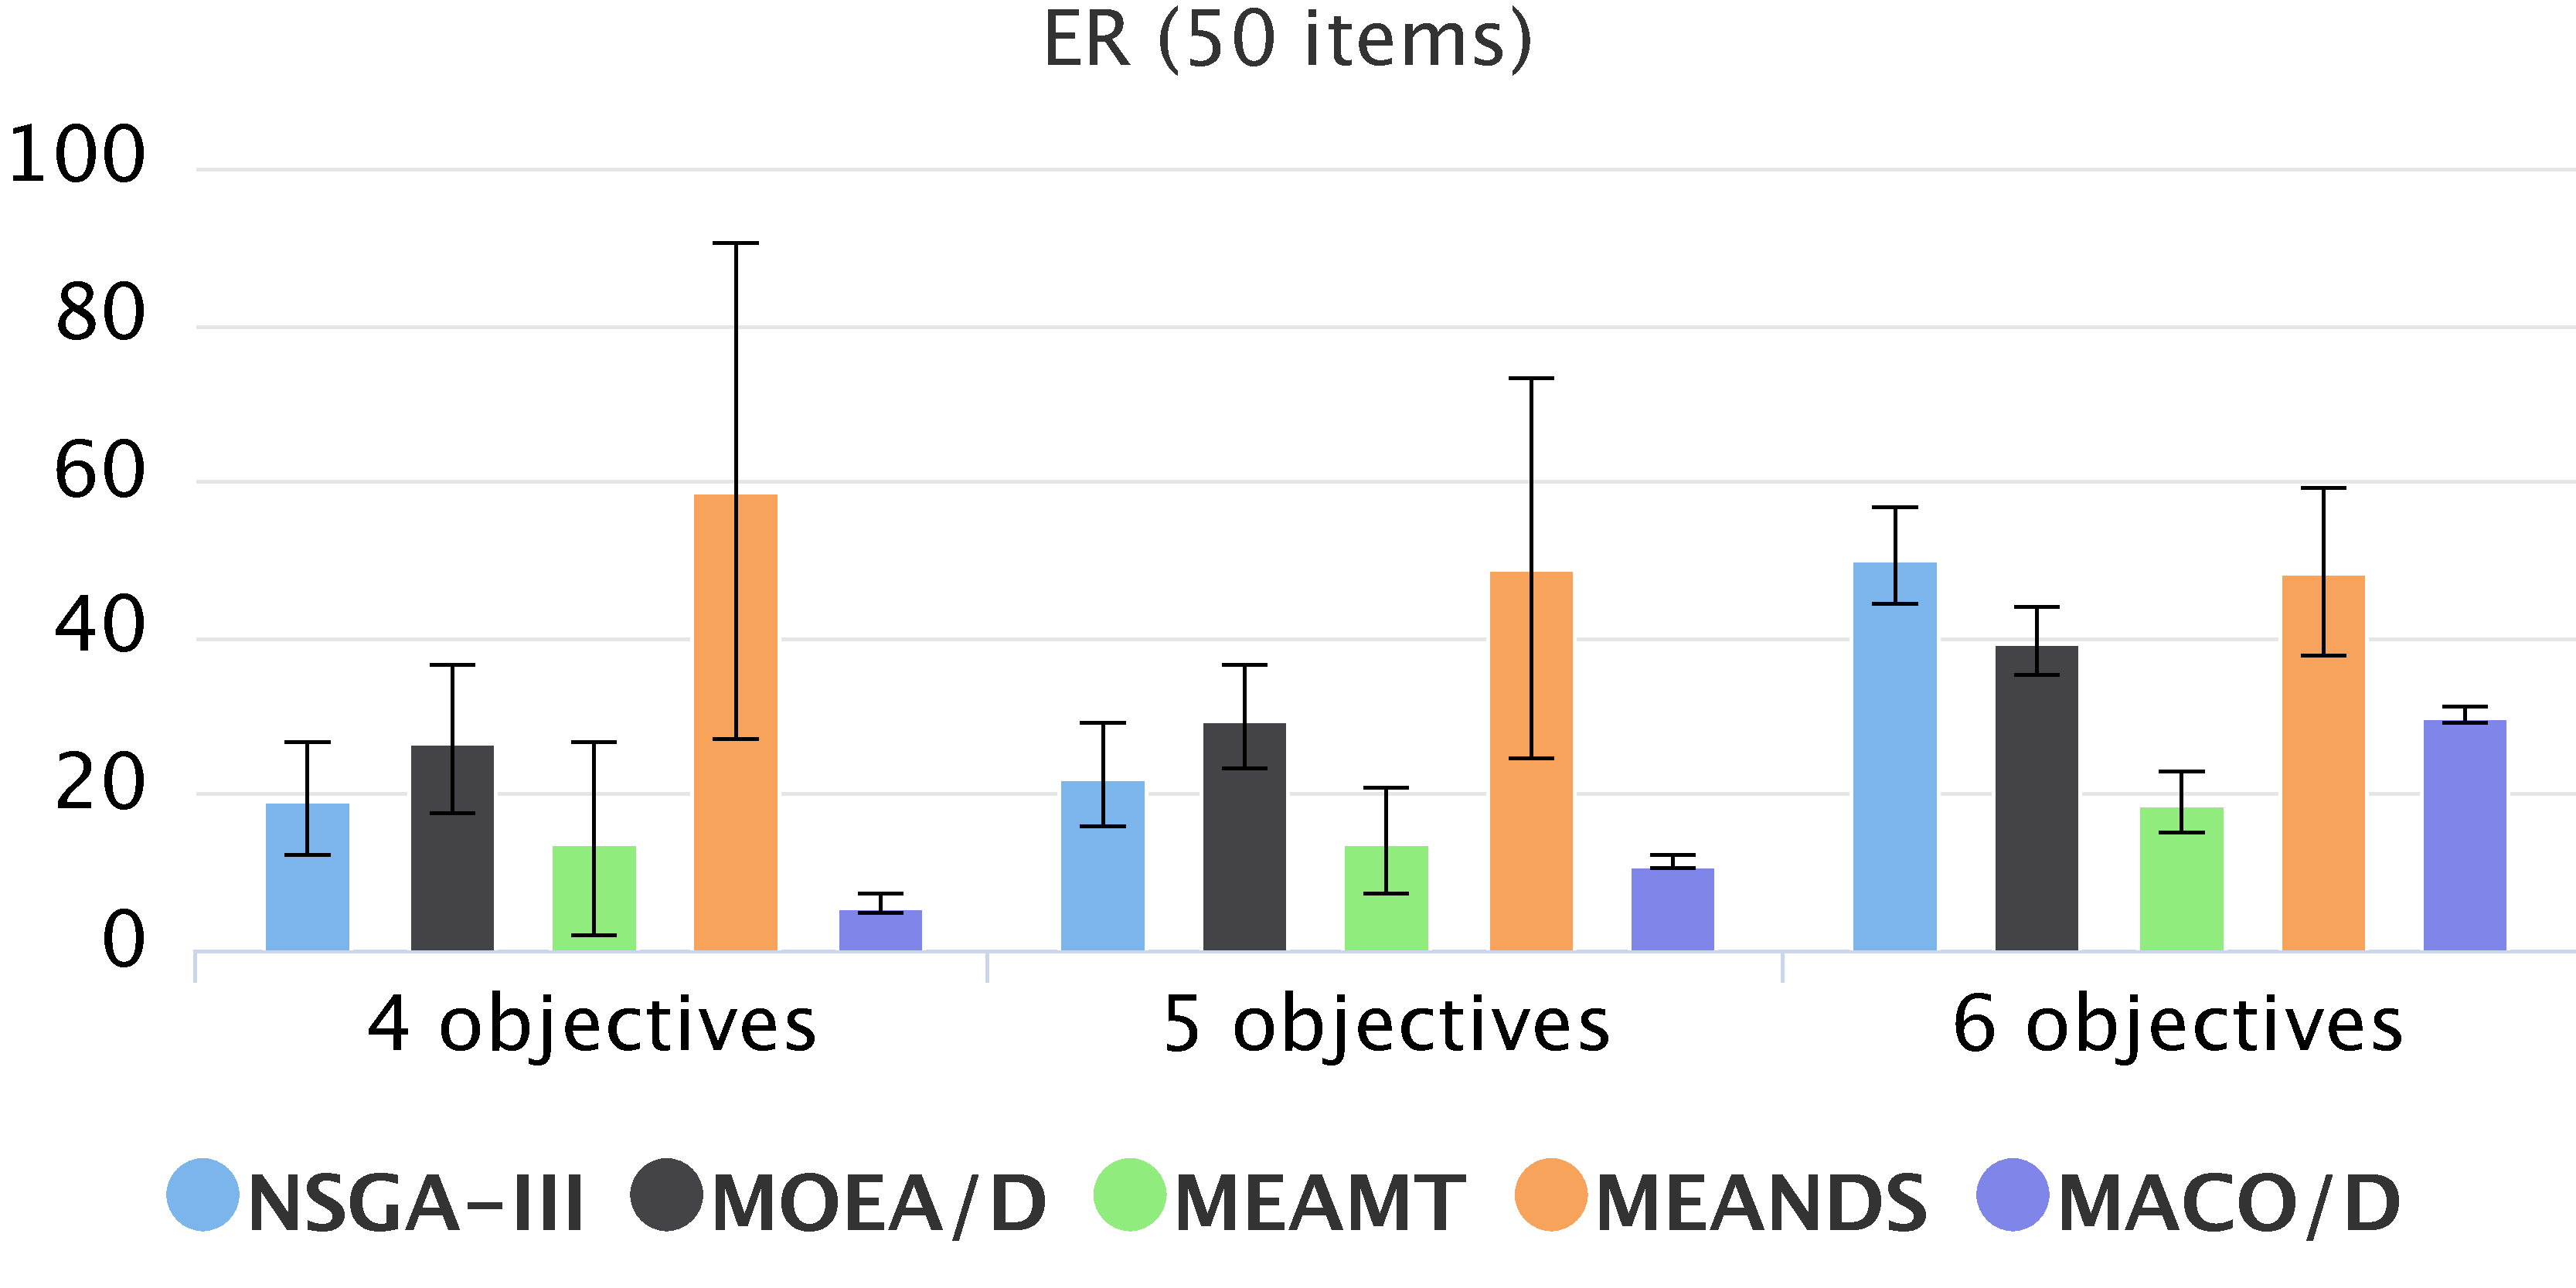
\includegraphics[width=0.5\textwidth]{cap_experimentos/figs/etapa2/er-mkp-50}
	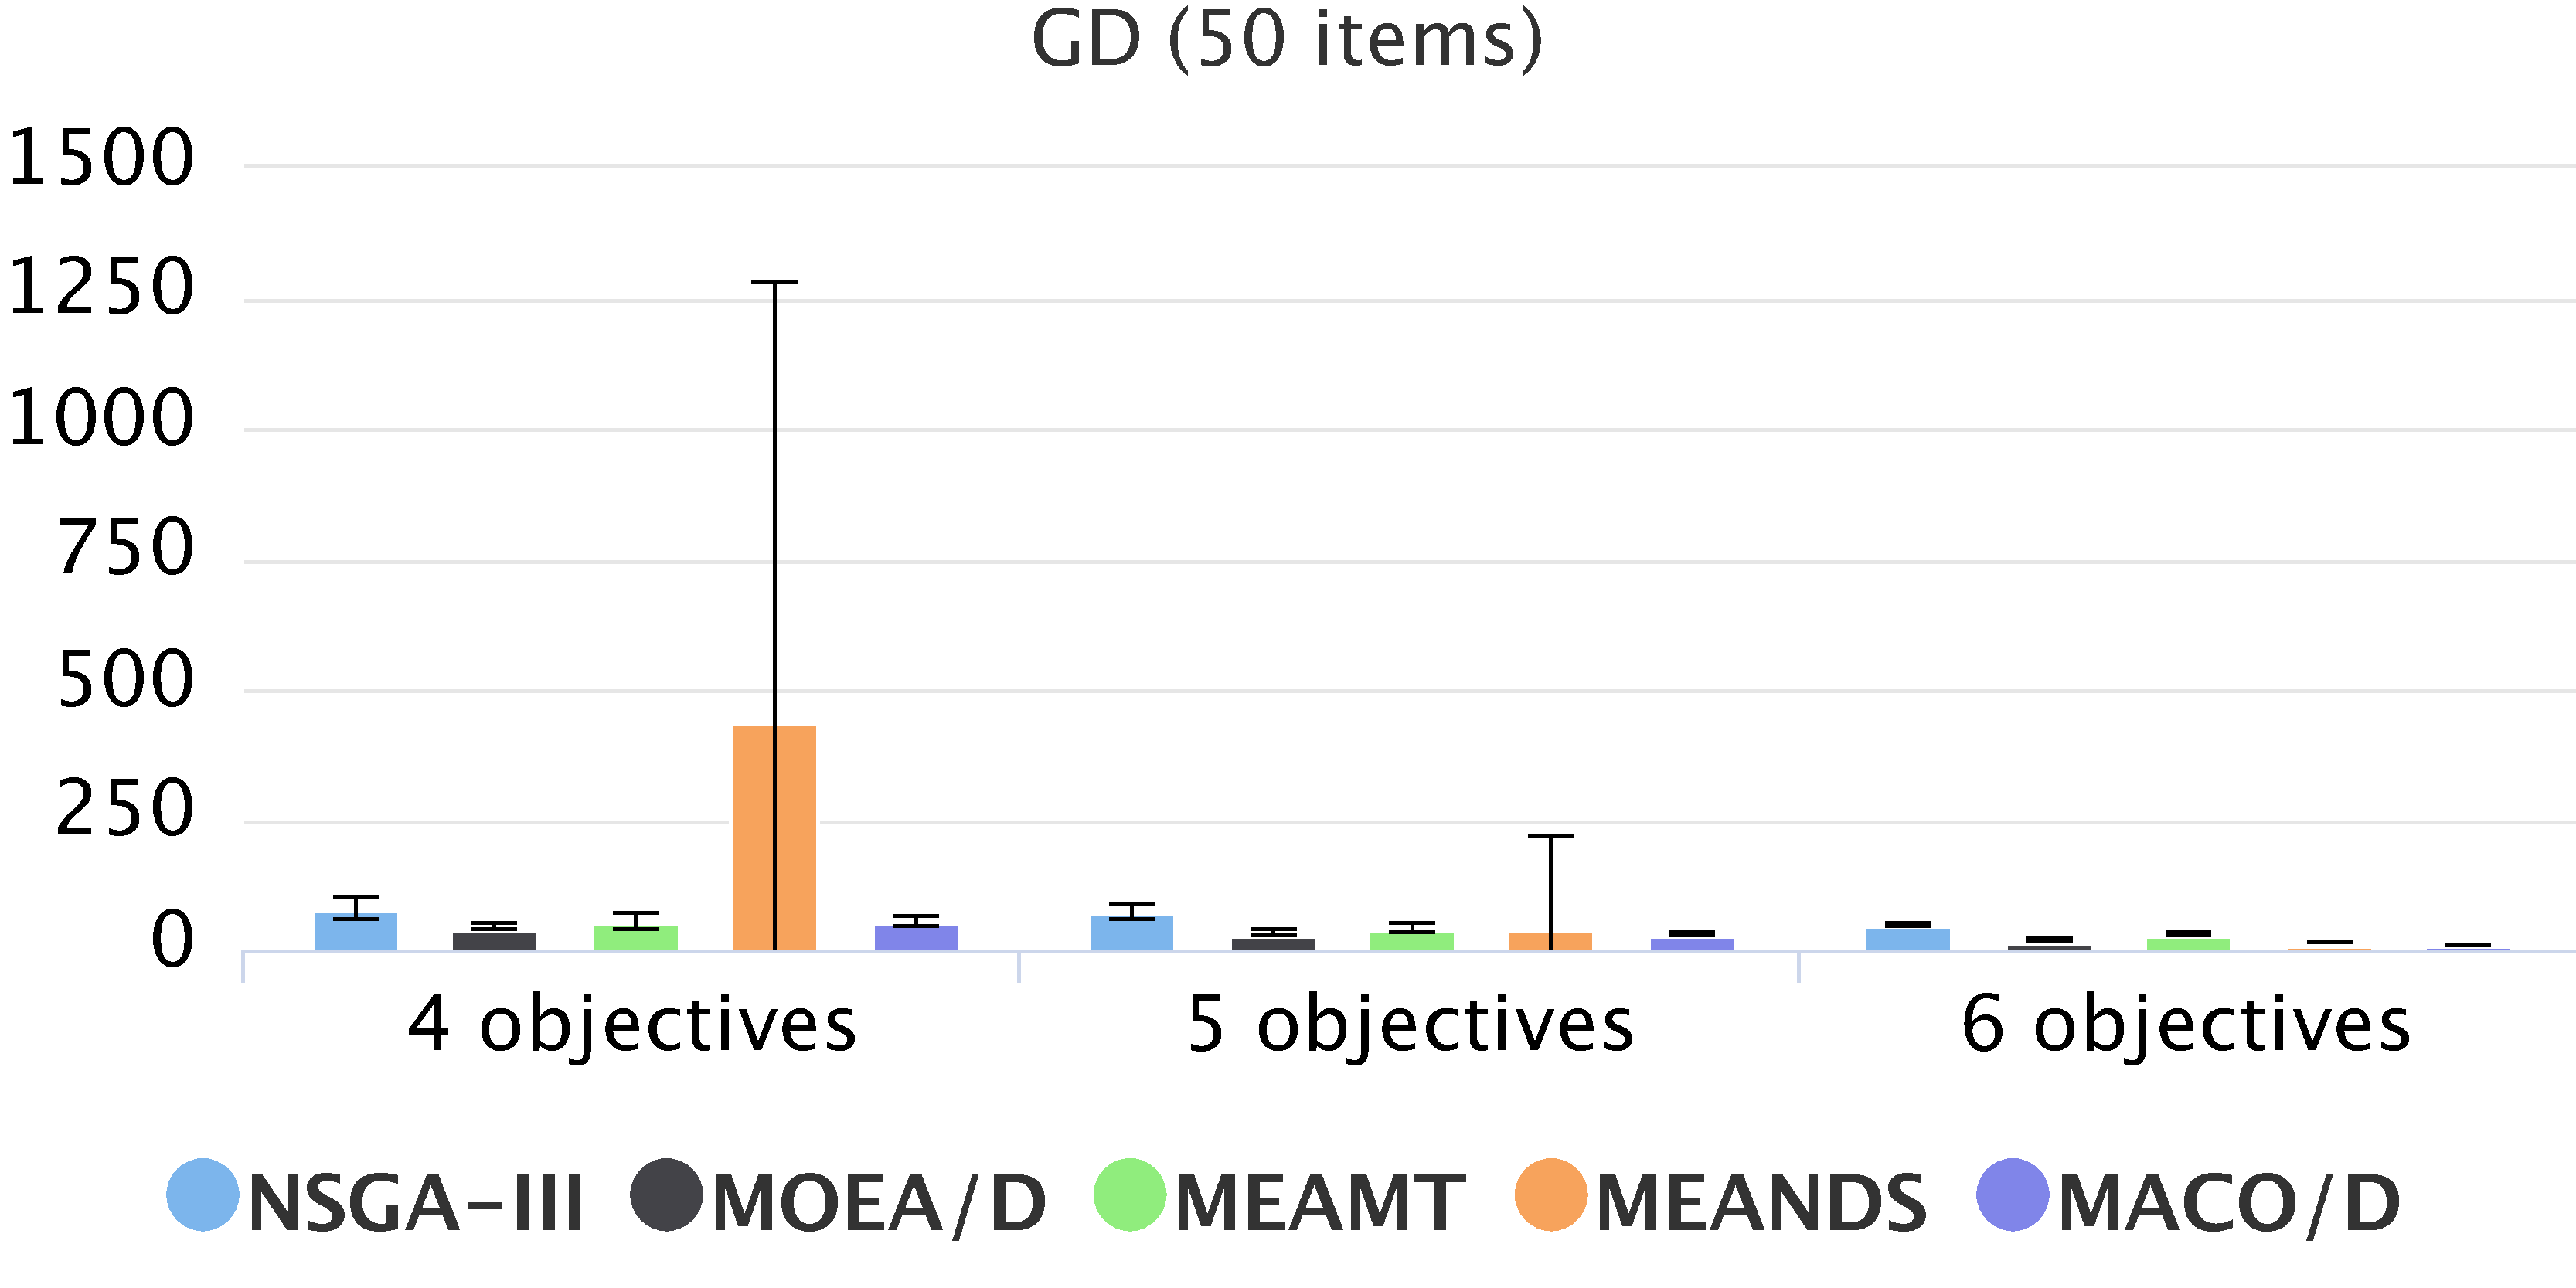
\includegraphics[width=0.5\textwidth]{cap_experimentos/figs/etapa2/gd-mkp-50}
	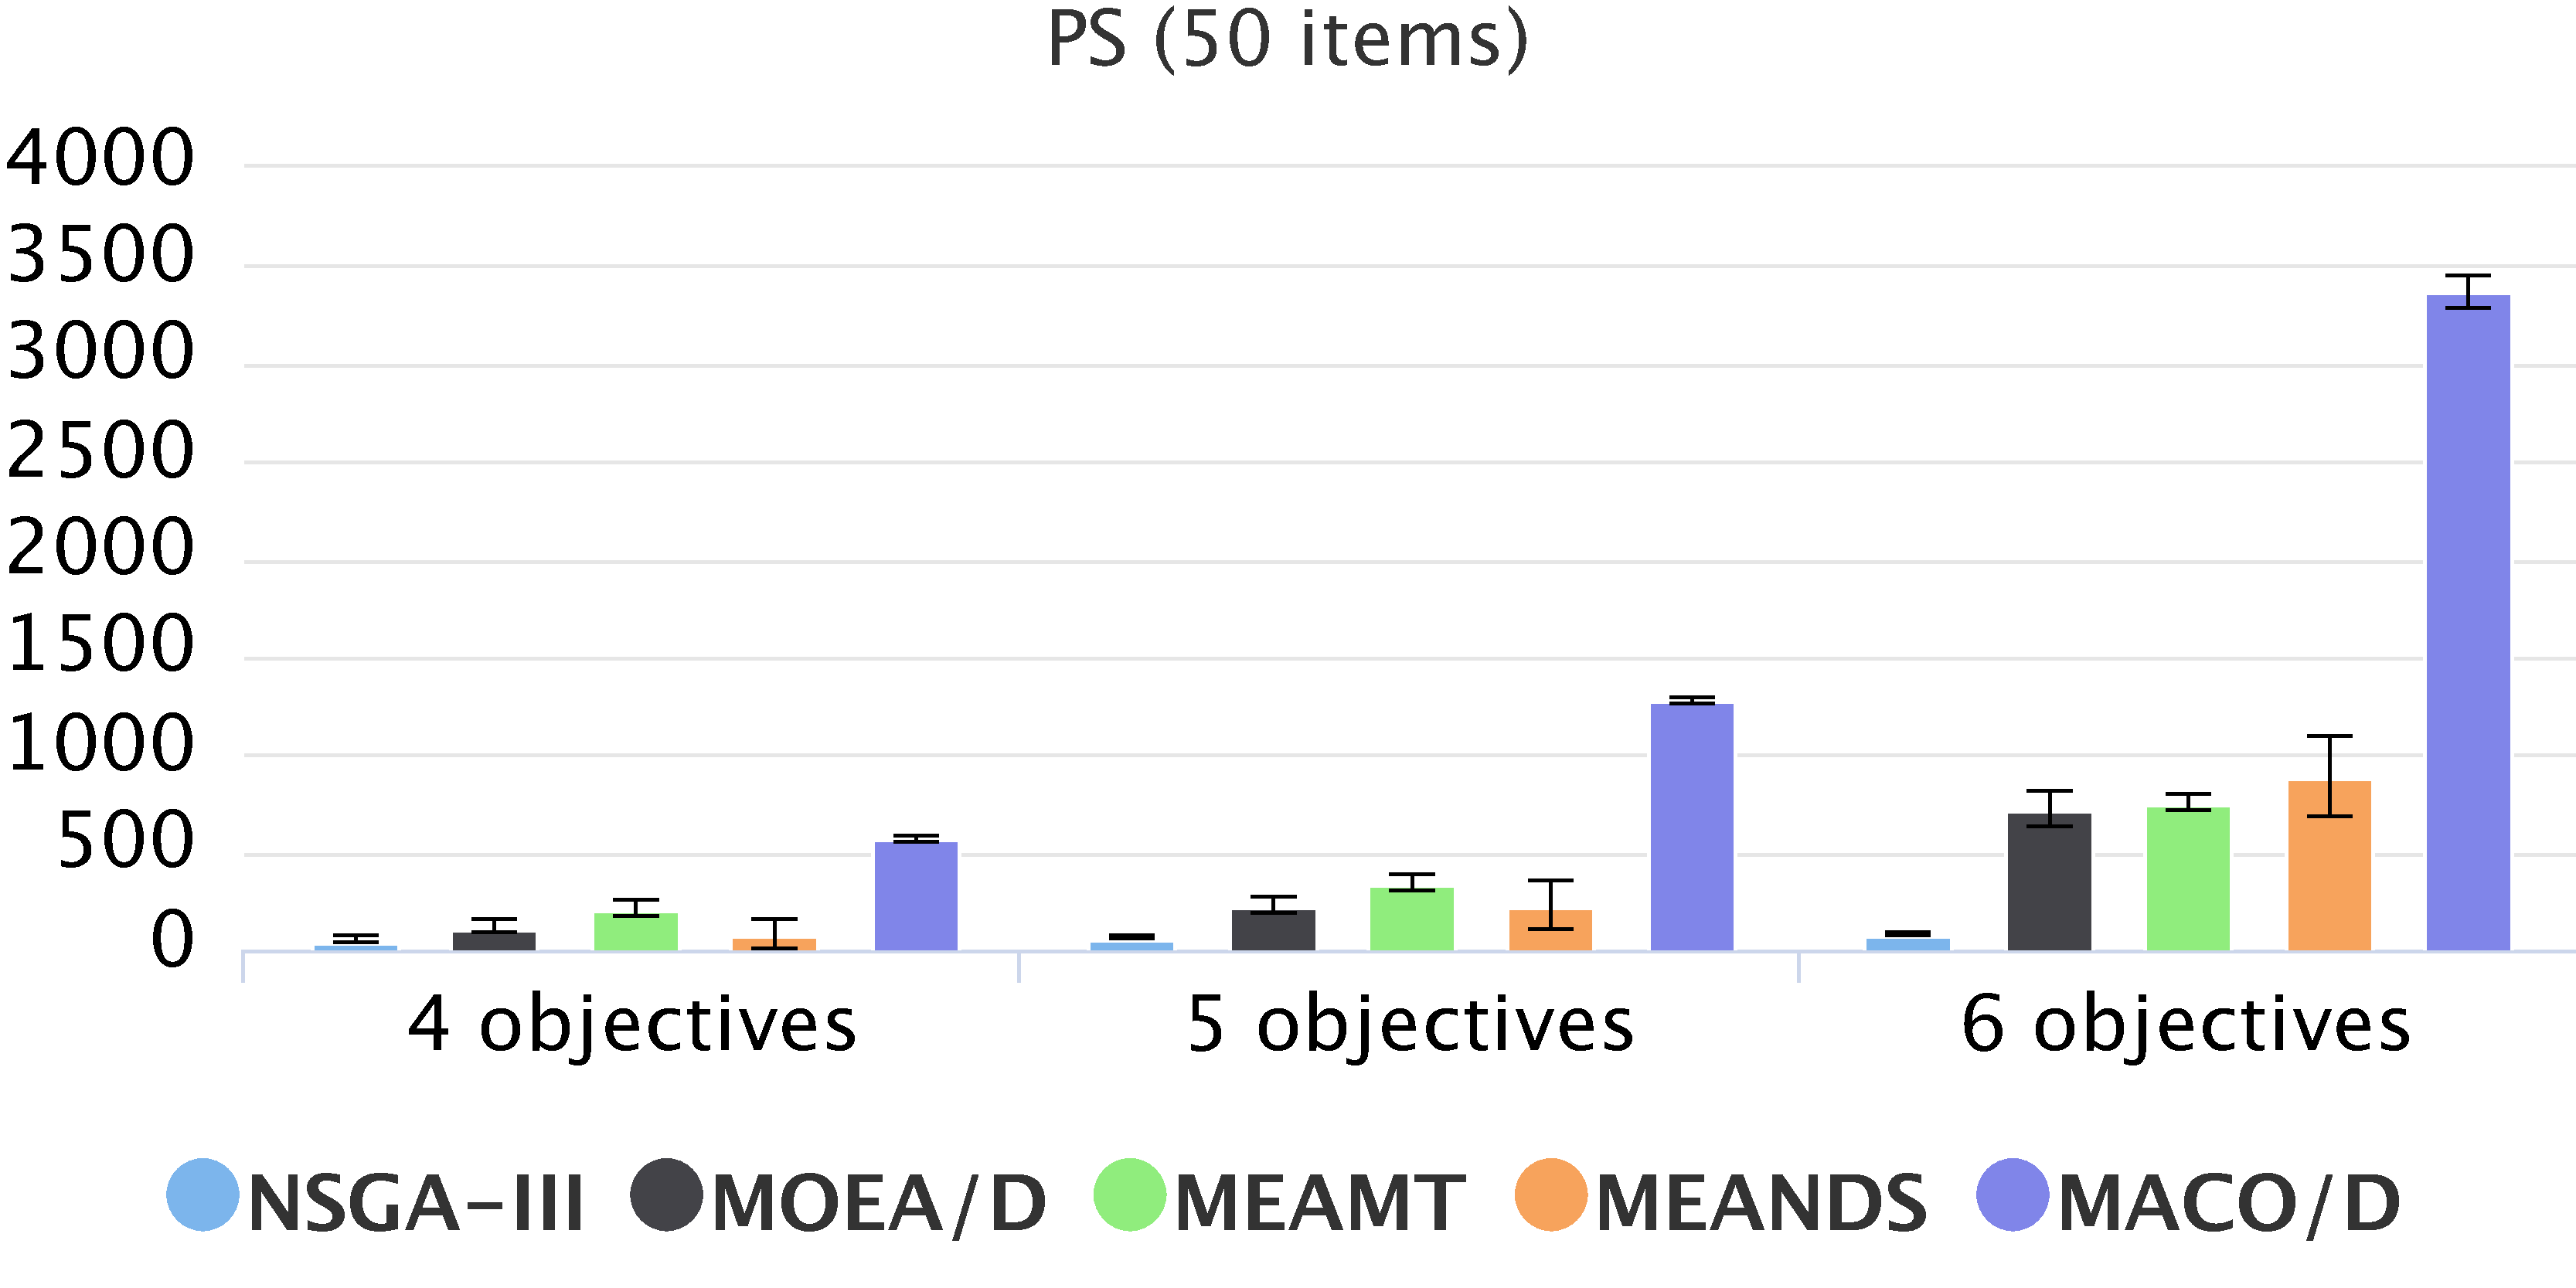
\includegraphics[width=0.5\textwidth]{cap_experimentos/figs/etapa2/ps-mkp-50}
	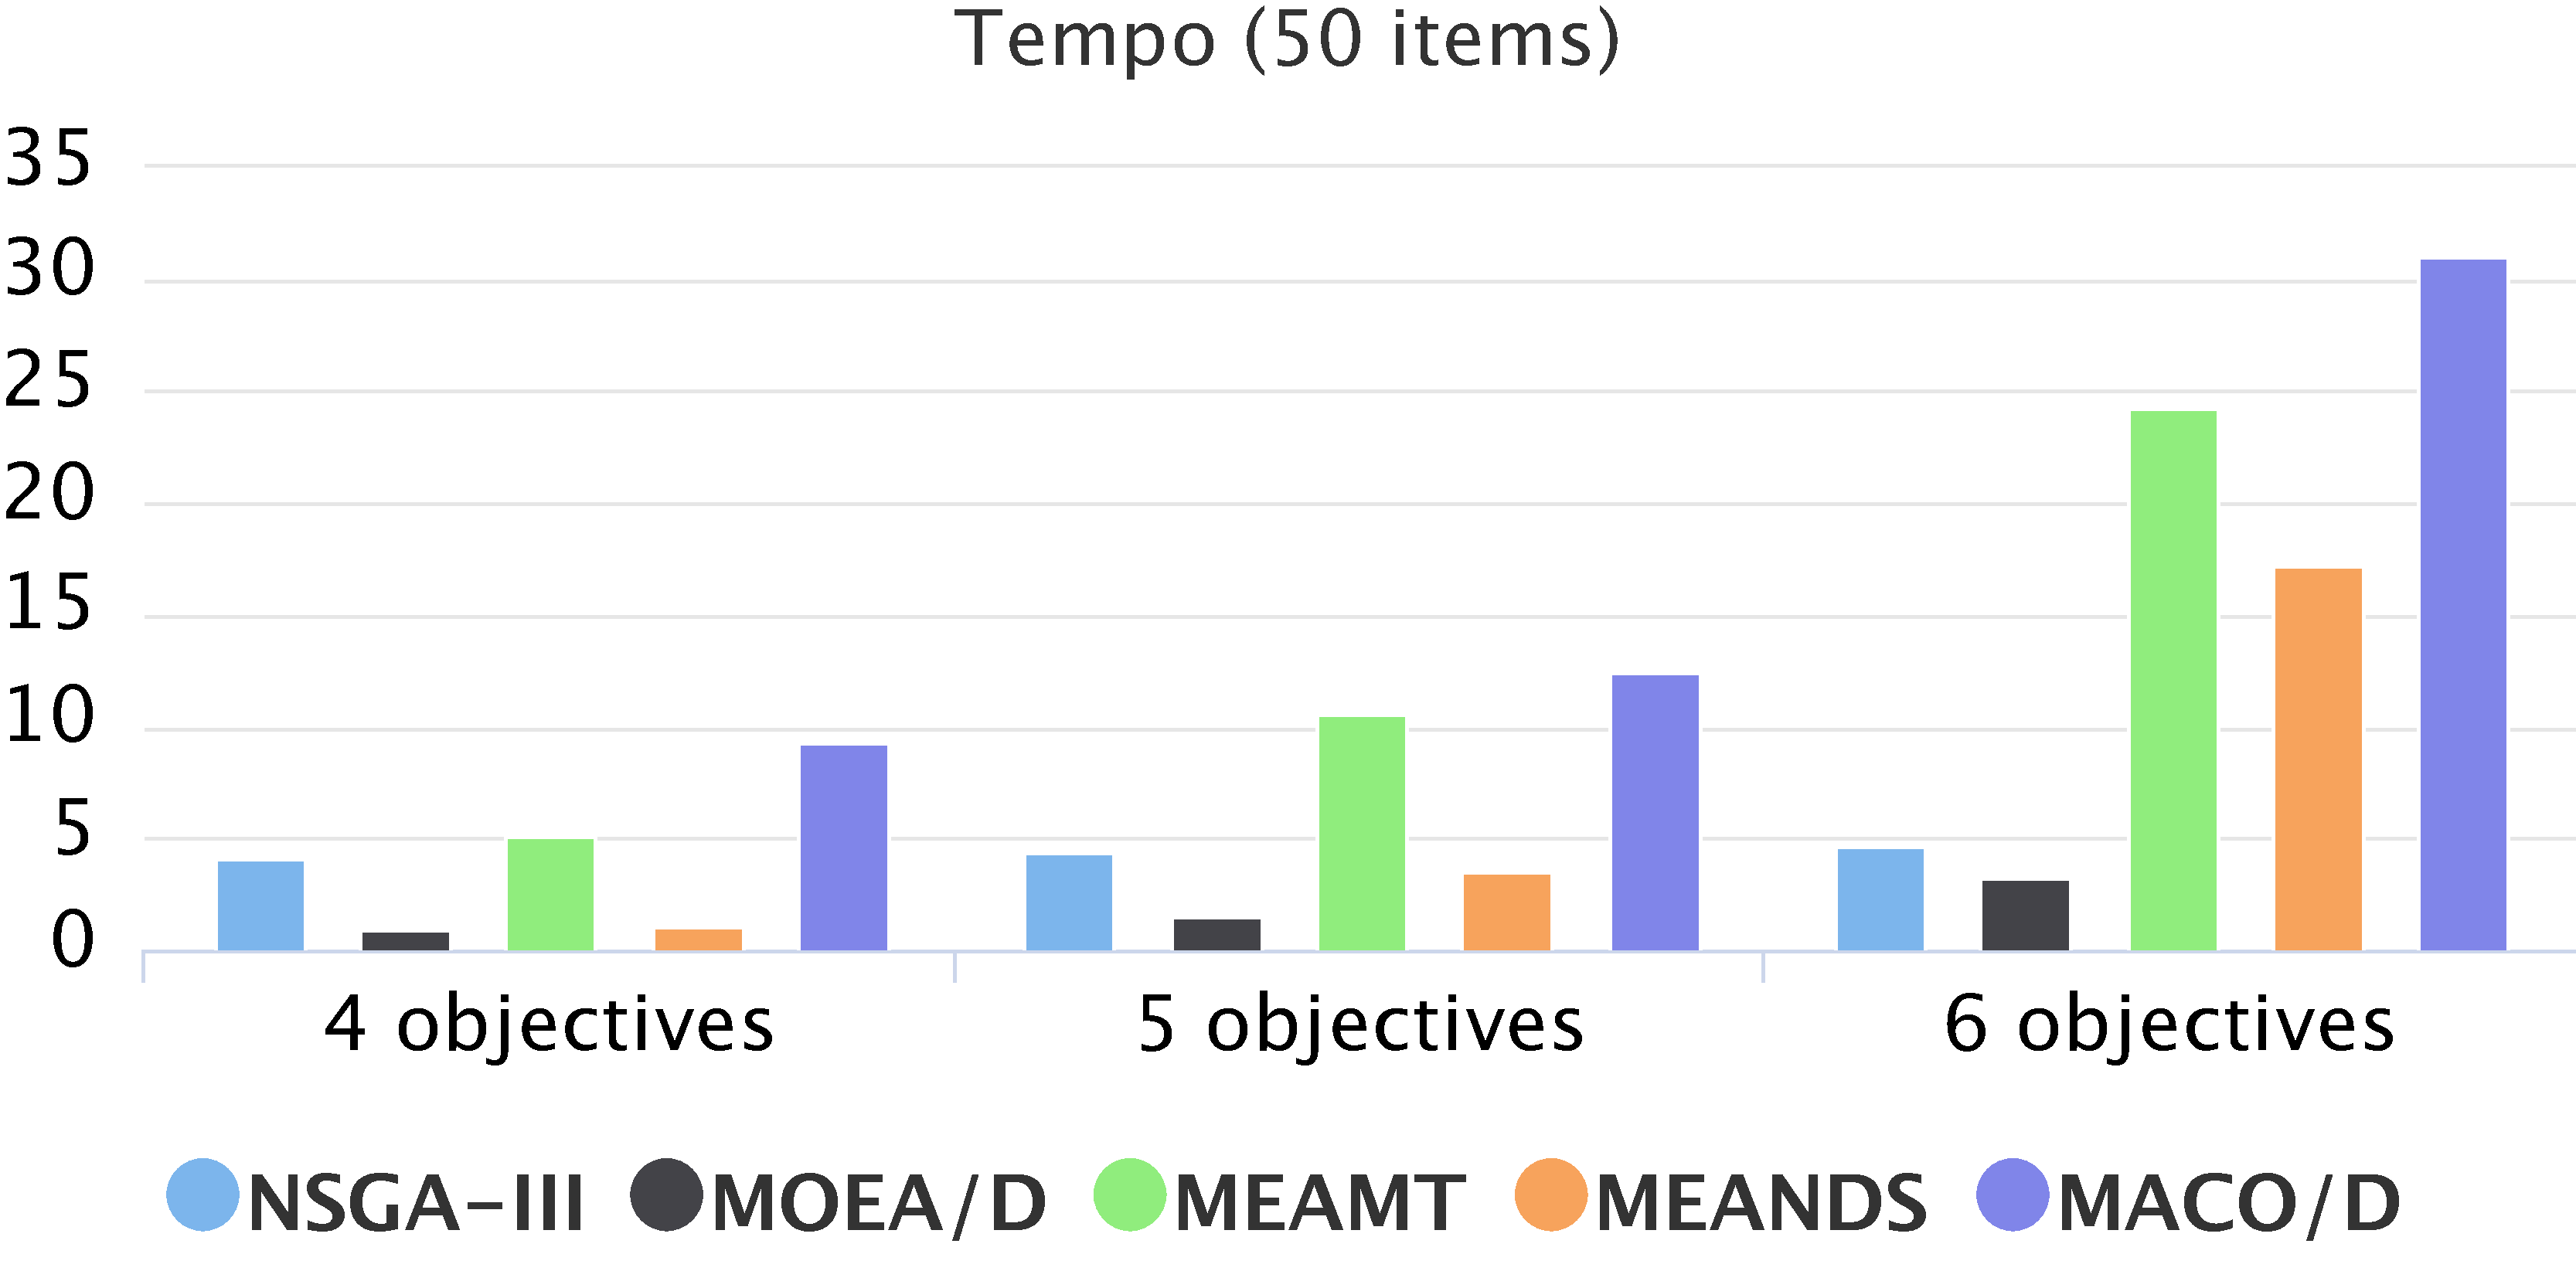
\includegraphics[width=0.5\textwidth]{cap_experimentos/figs/etapa2/time-mkp-50}
\end{figure*}

Análise do MKP-50

\begin{figure*}[!htbp]
	\caption{Etapa 2: resultados agrupados para o PMM com 30, 40 e 50 itens}
	\label{fig_exp2_mkp_todos}
	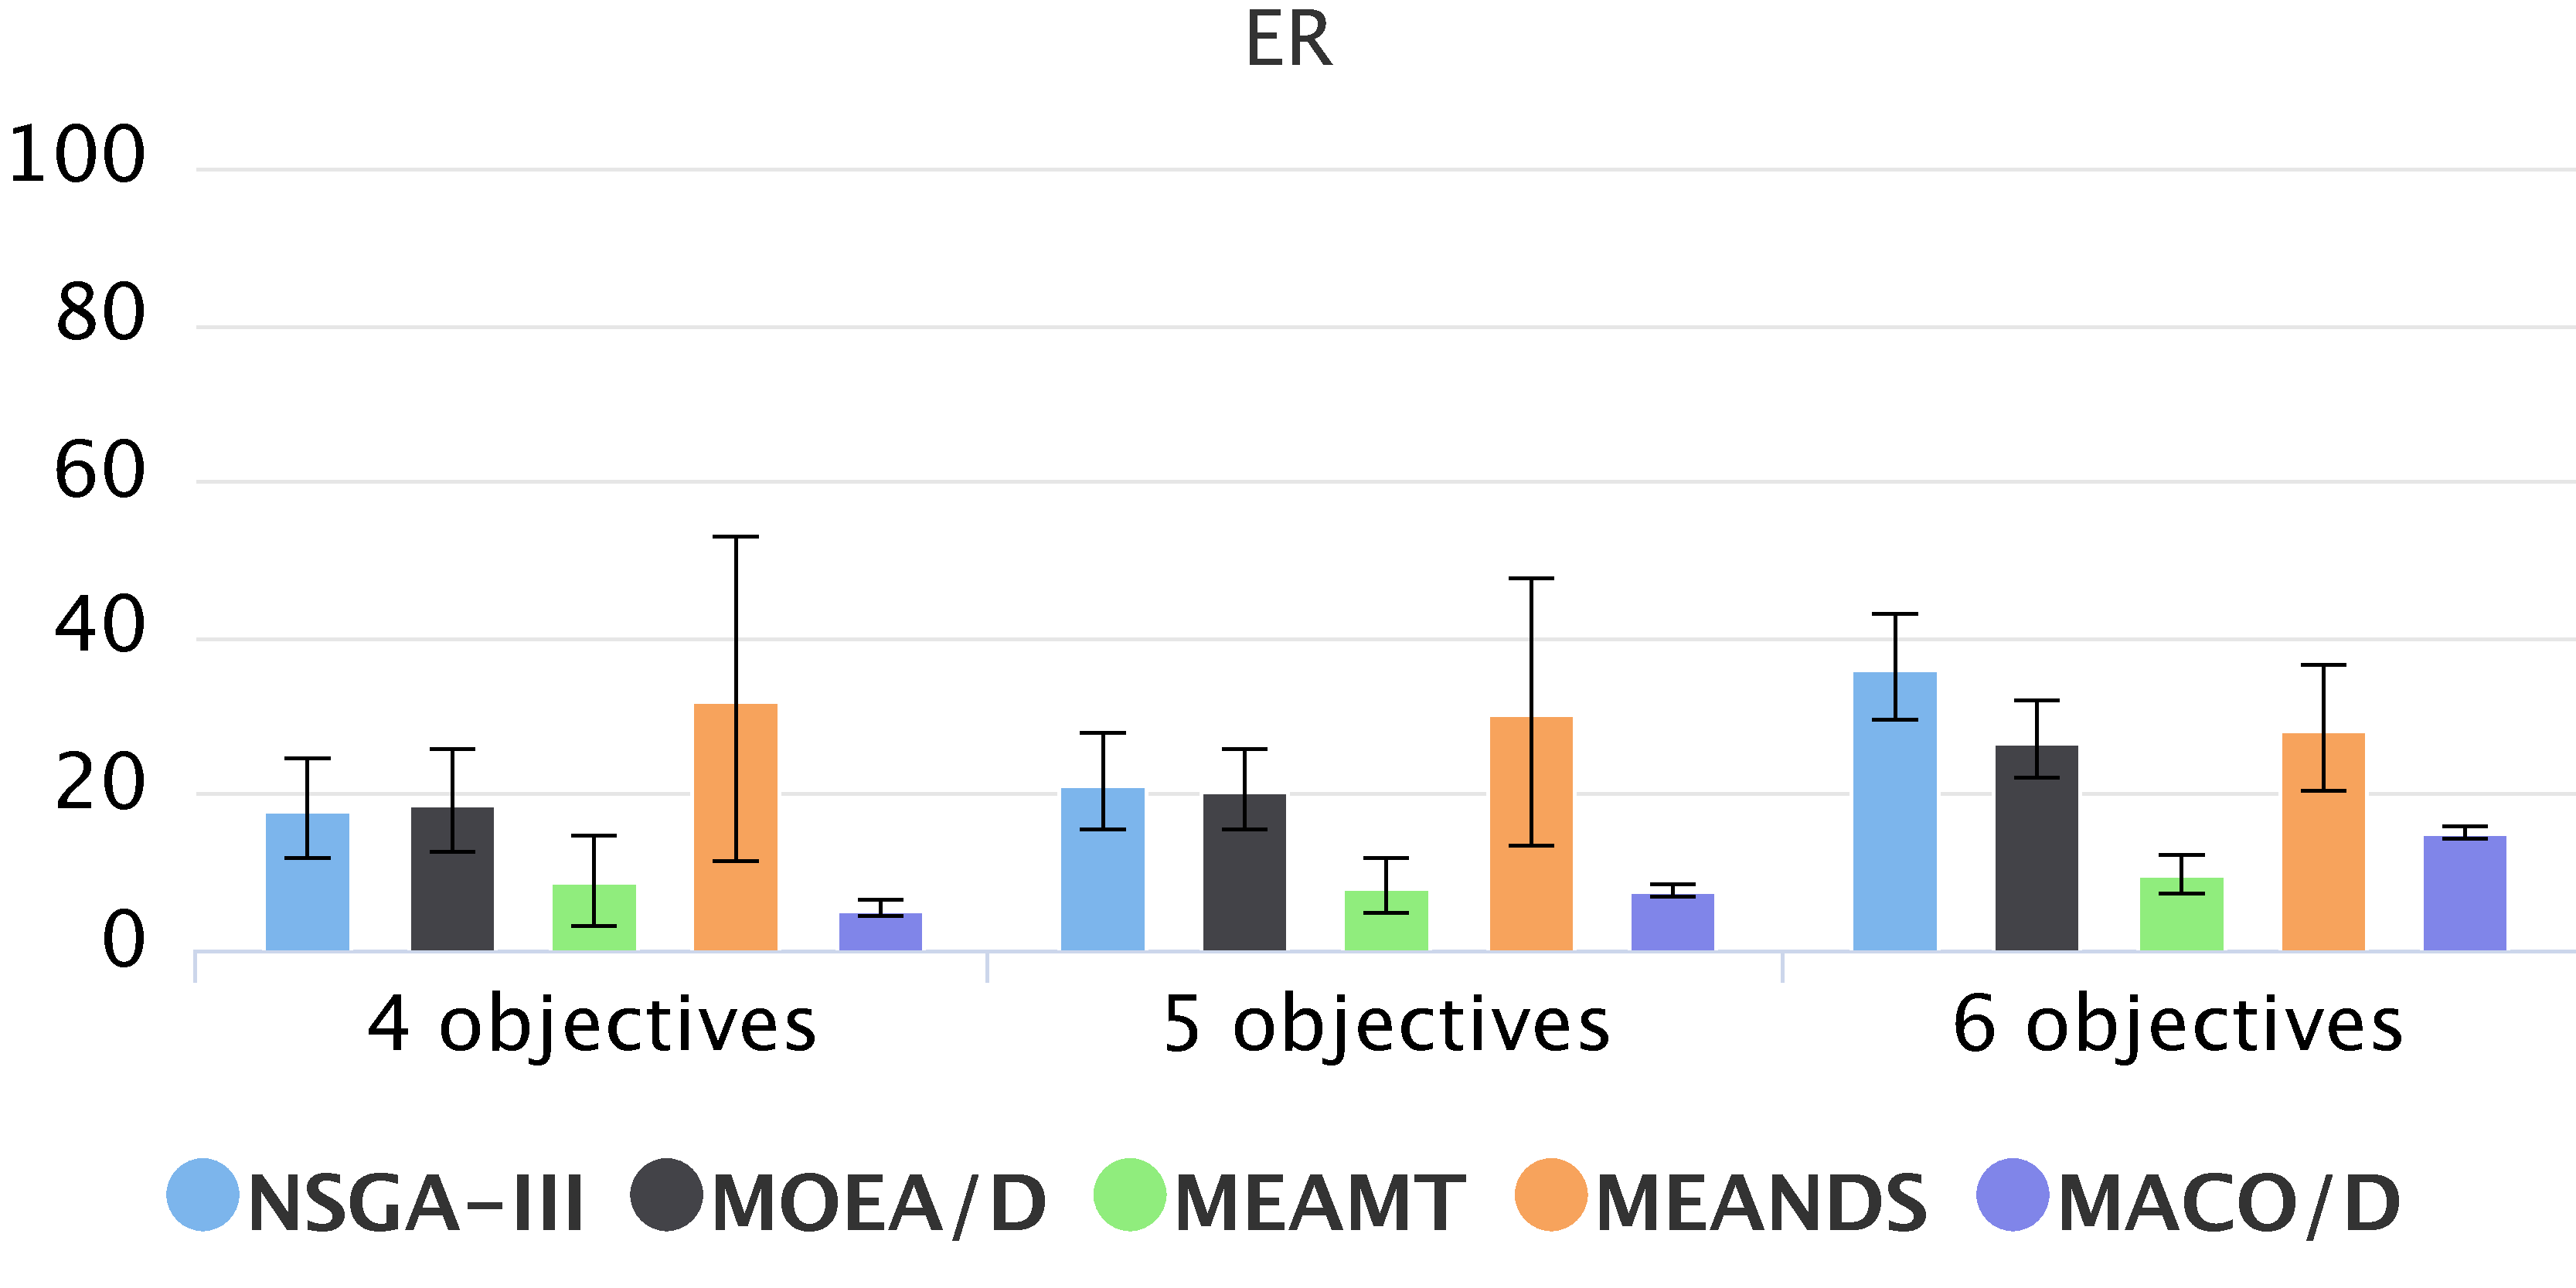
\includegraphics[width=0.5\textwidth]{cap_experimentos/figs/etapa2/er-mkp-todos}
	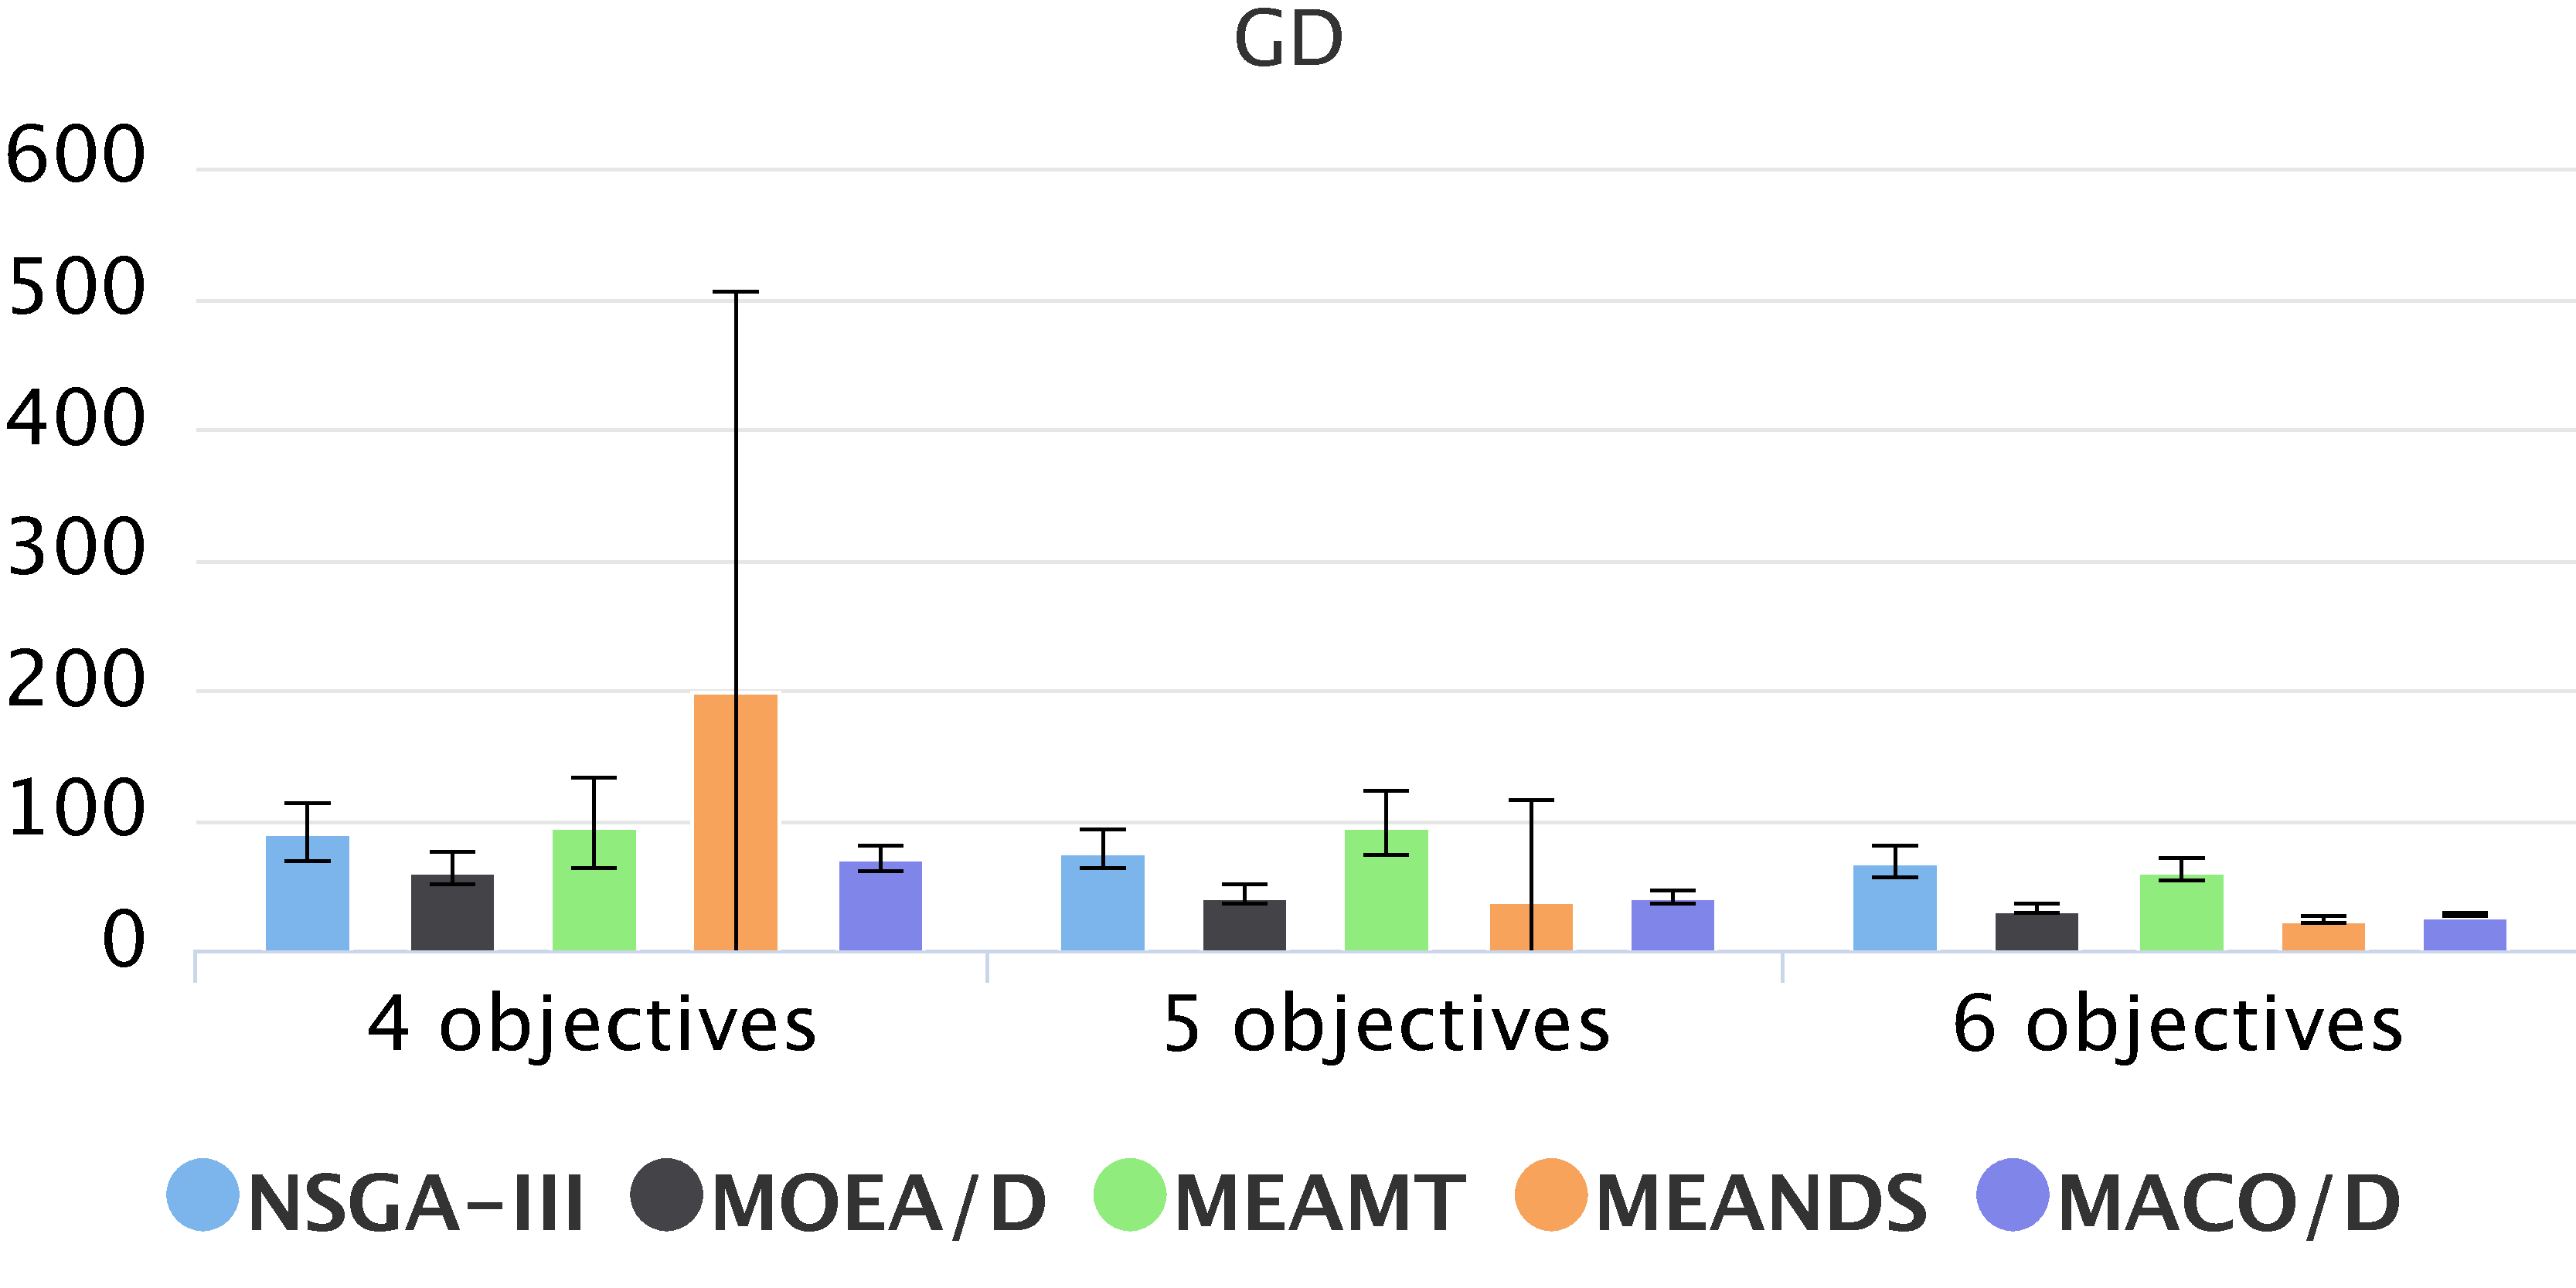
\includegraphics[width=0.5\textwidth]{cap_experimentos/figs/etapa2/gd-mkp-todos}
	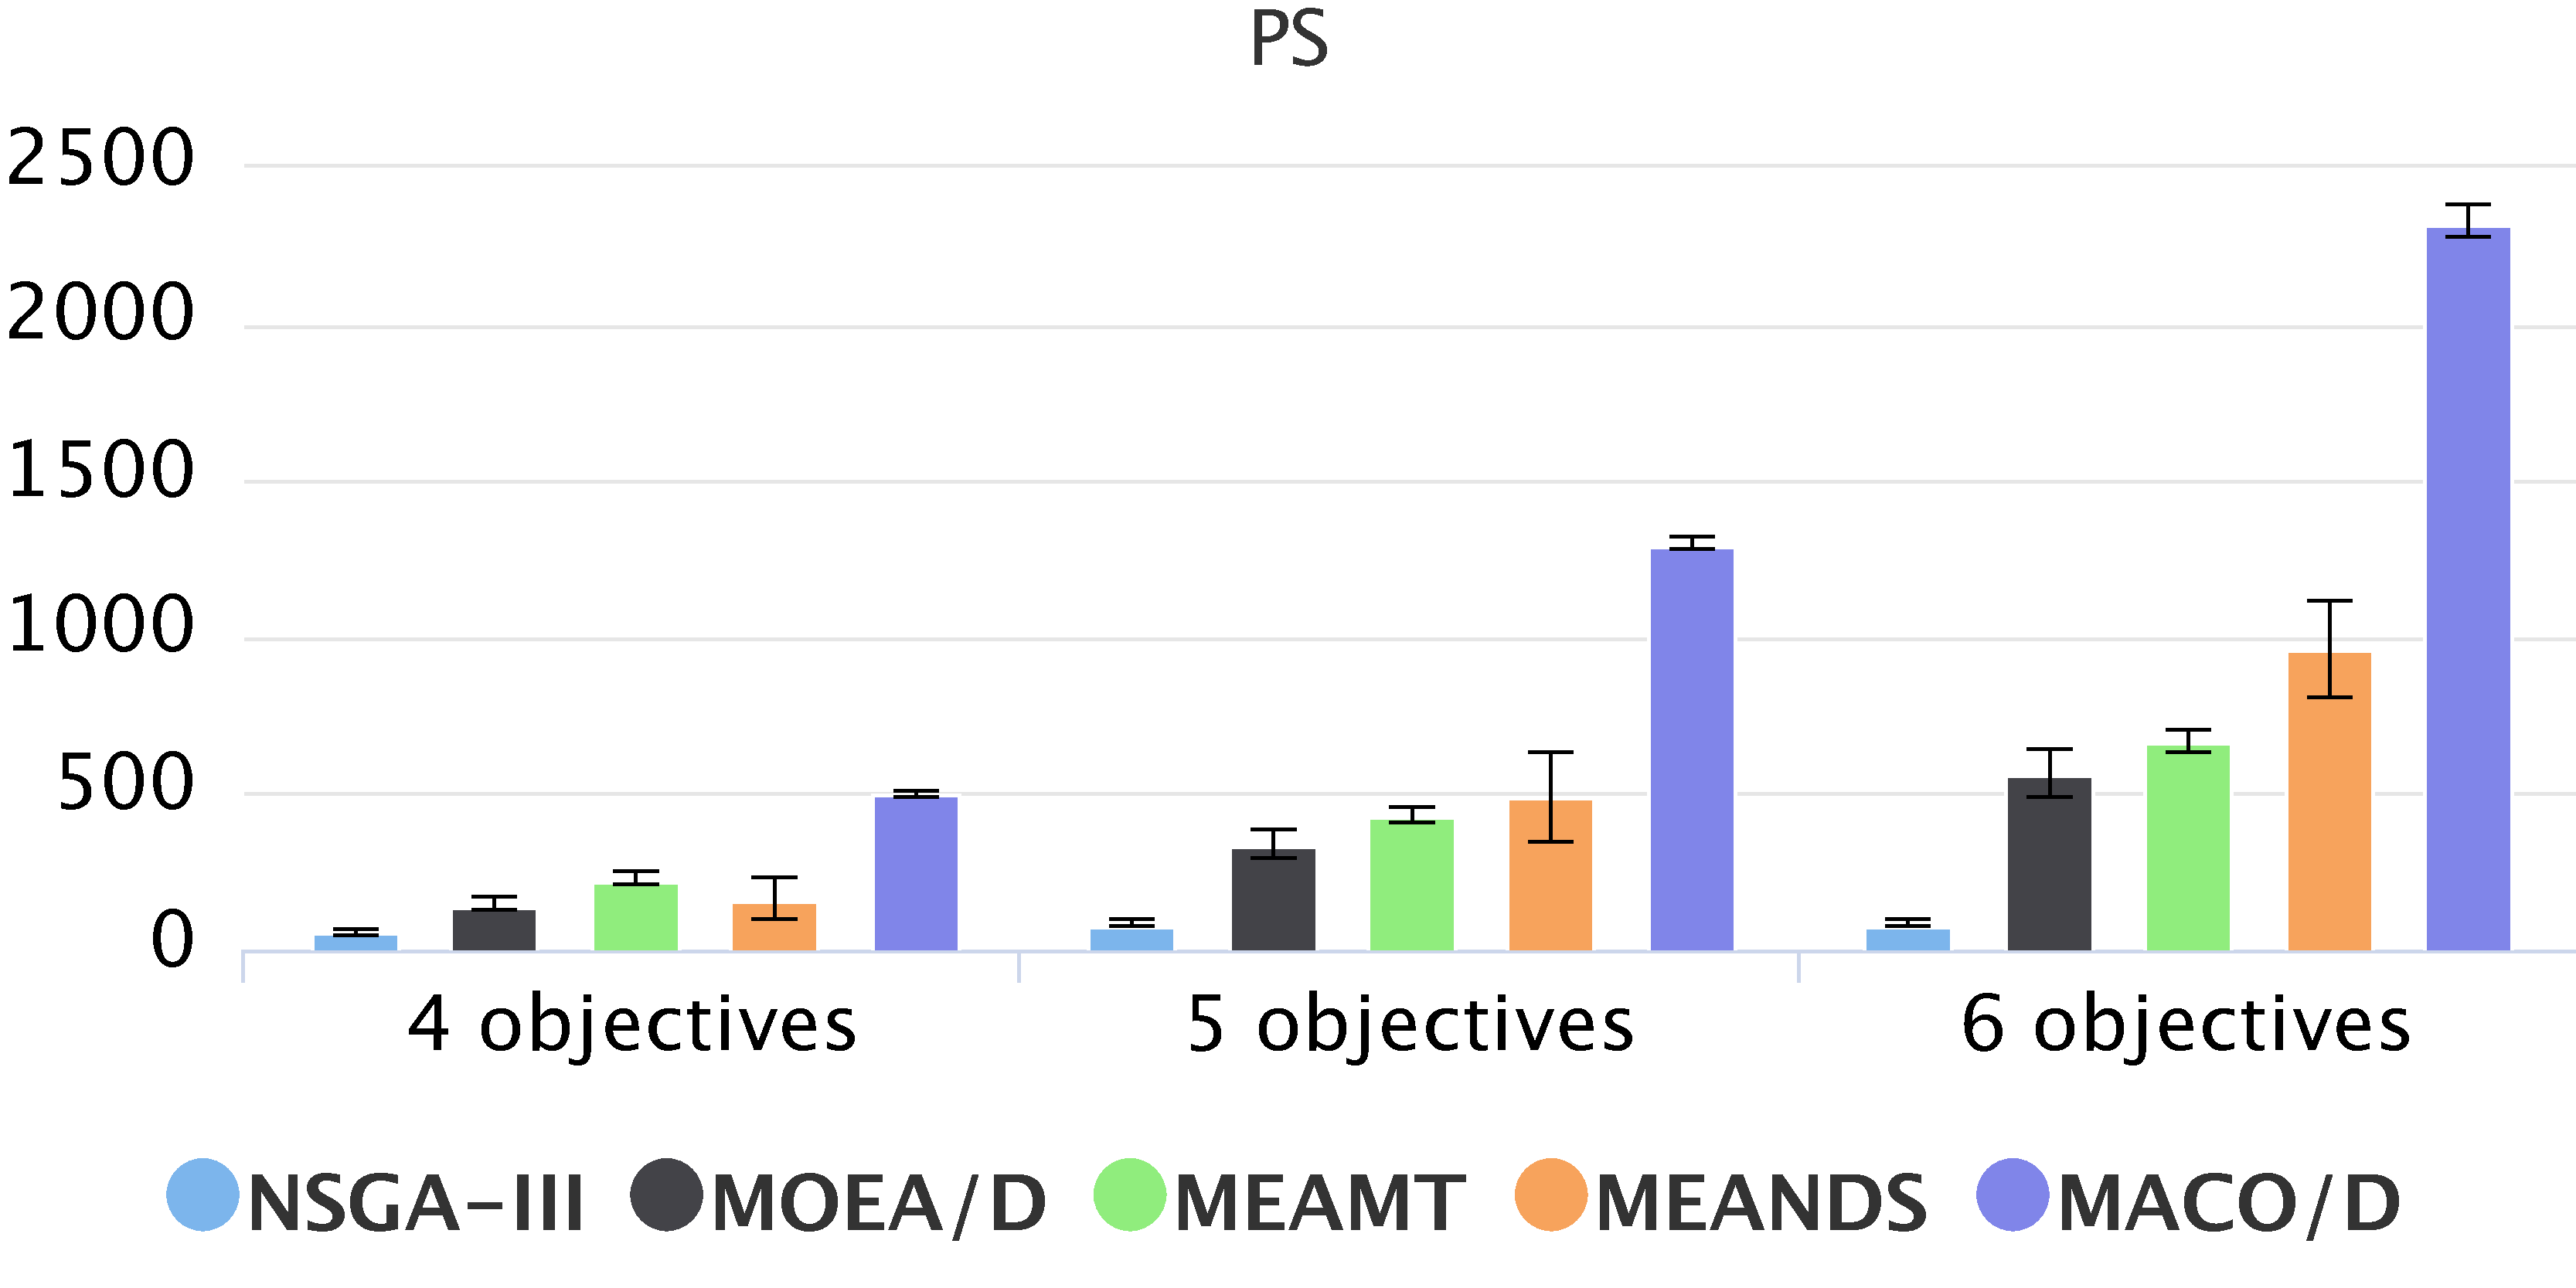
\includegraphics[width=0.5\textwidth]{cap_experimentos/figs/etapa2/ps-mkp-todos}
	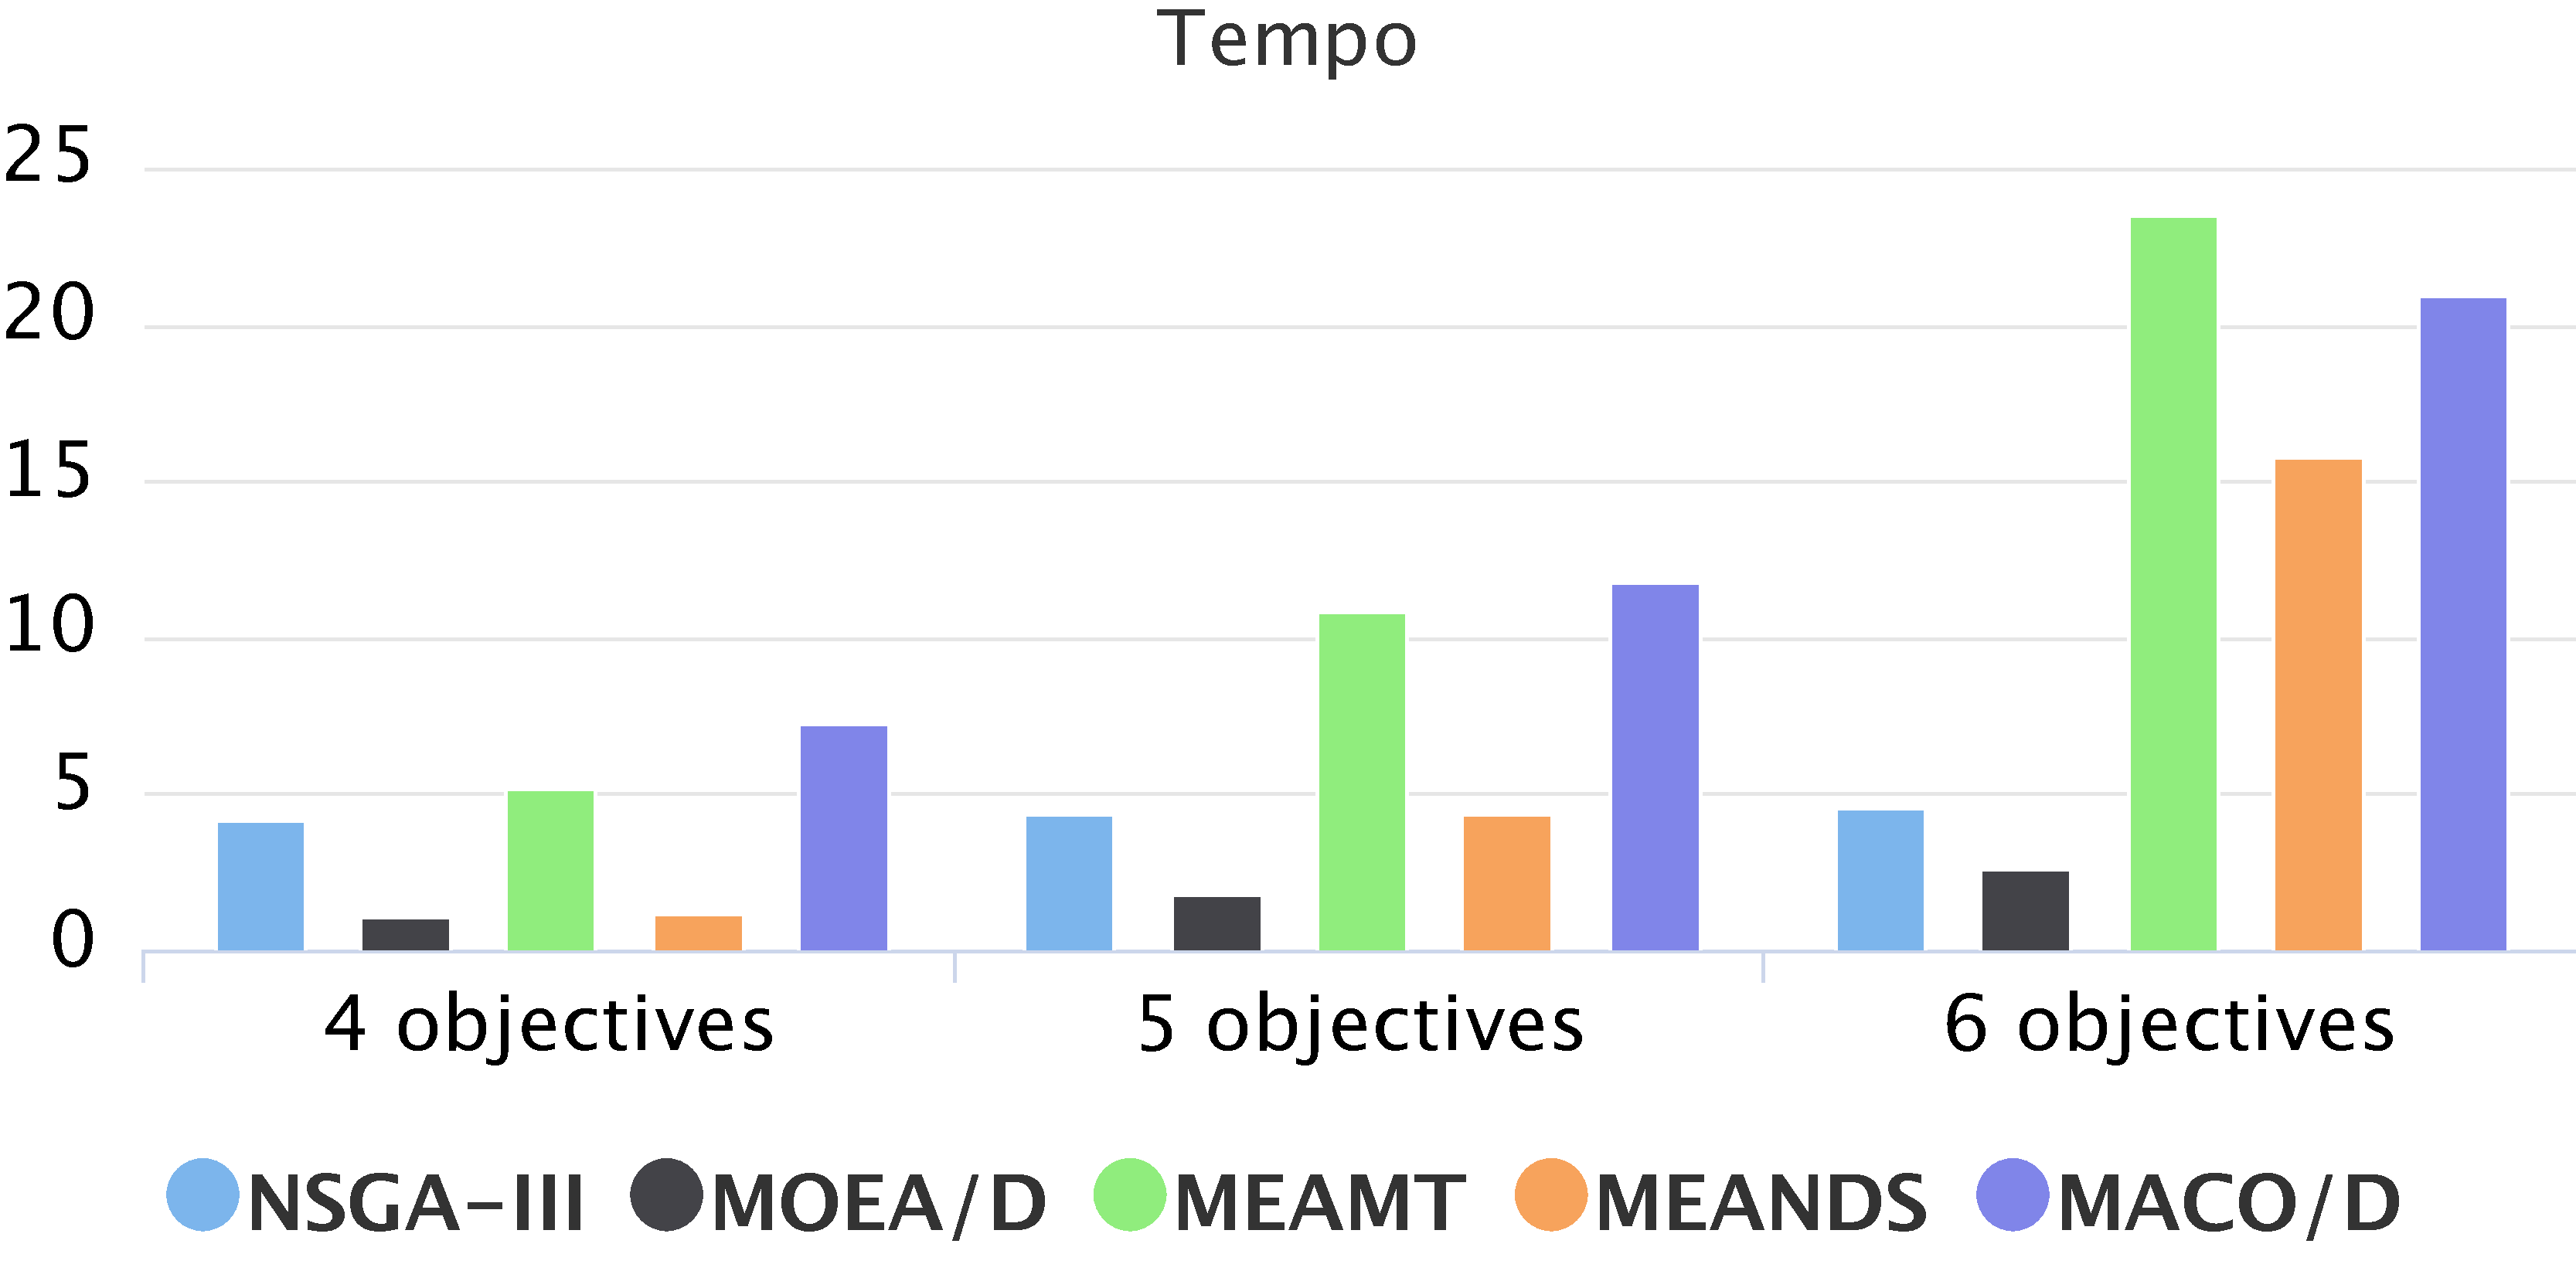
\includegraphics[width=0.5\textwidth]{cap_experimentos/figs/etapa2/time-mkp-todos}
\end{figure*}

Análise geral do MKP

\begin{figure*}[!htbp]
	\caption{Etapa 2: resultados para o PRM na rede $R_1$}
	\label{fig_exp2_mrp_r1}
	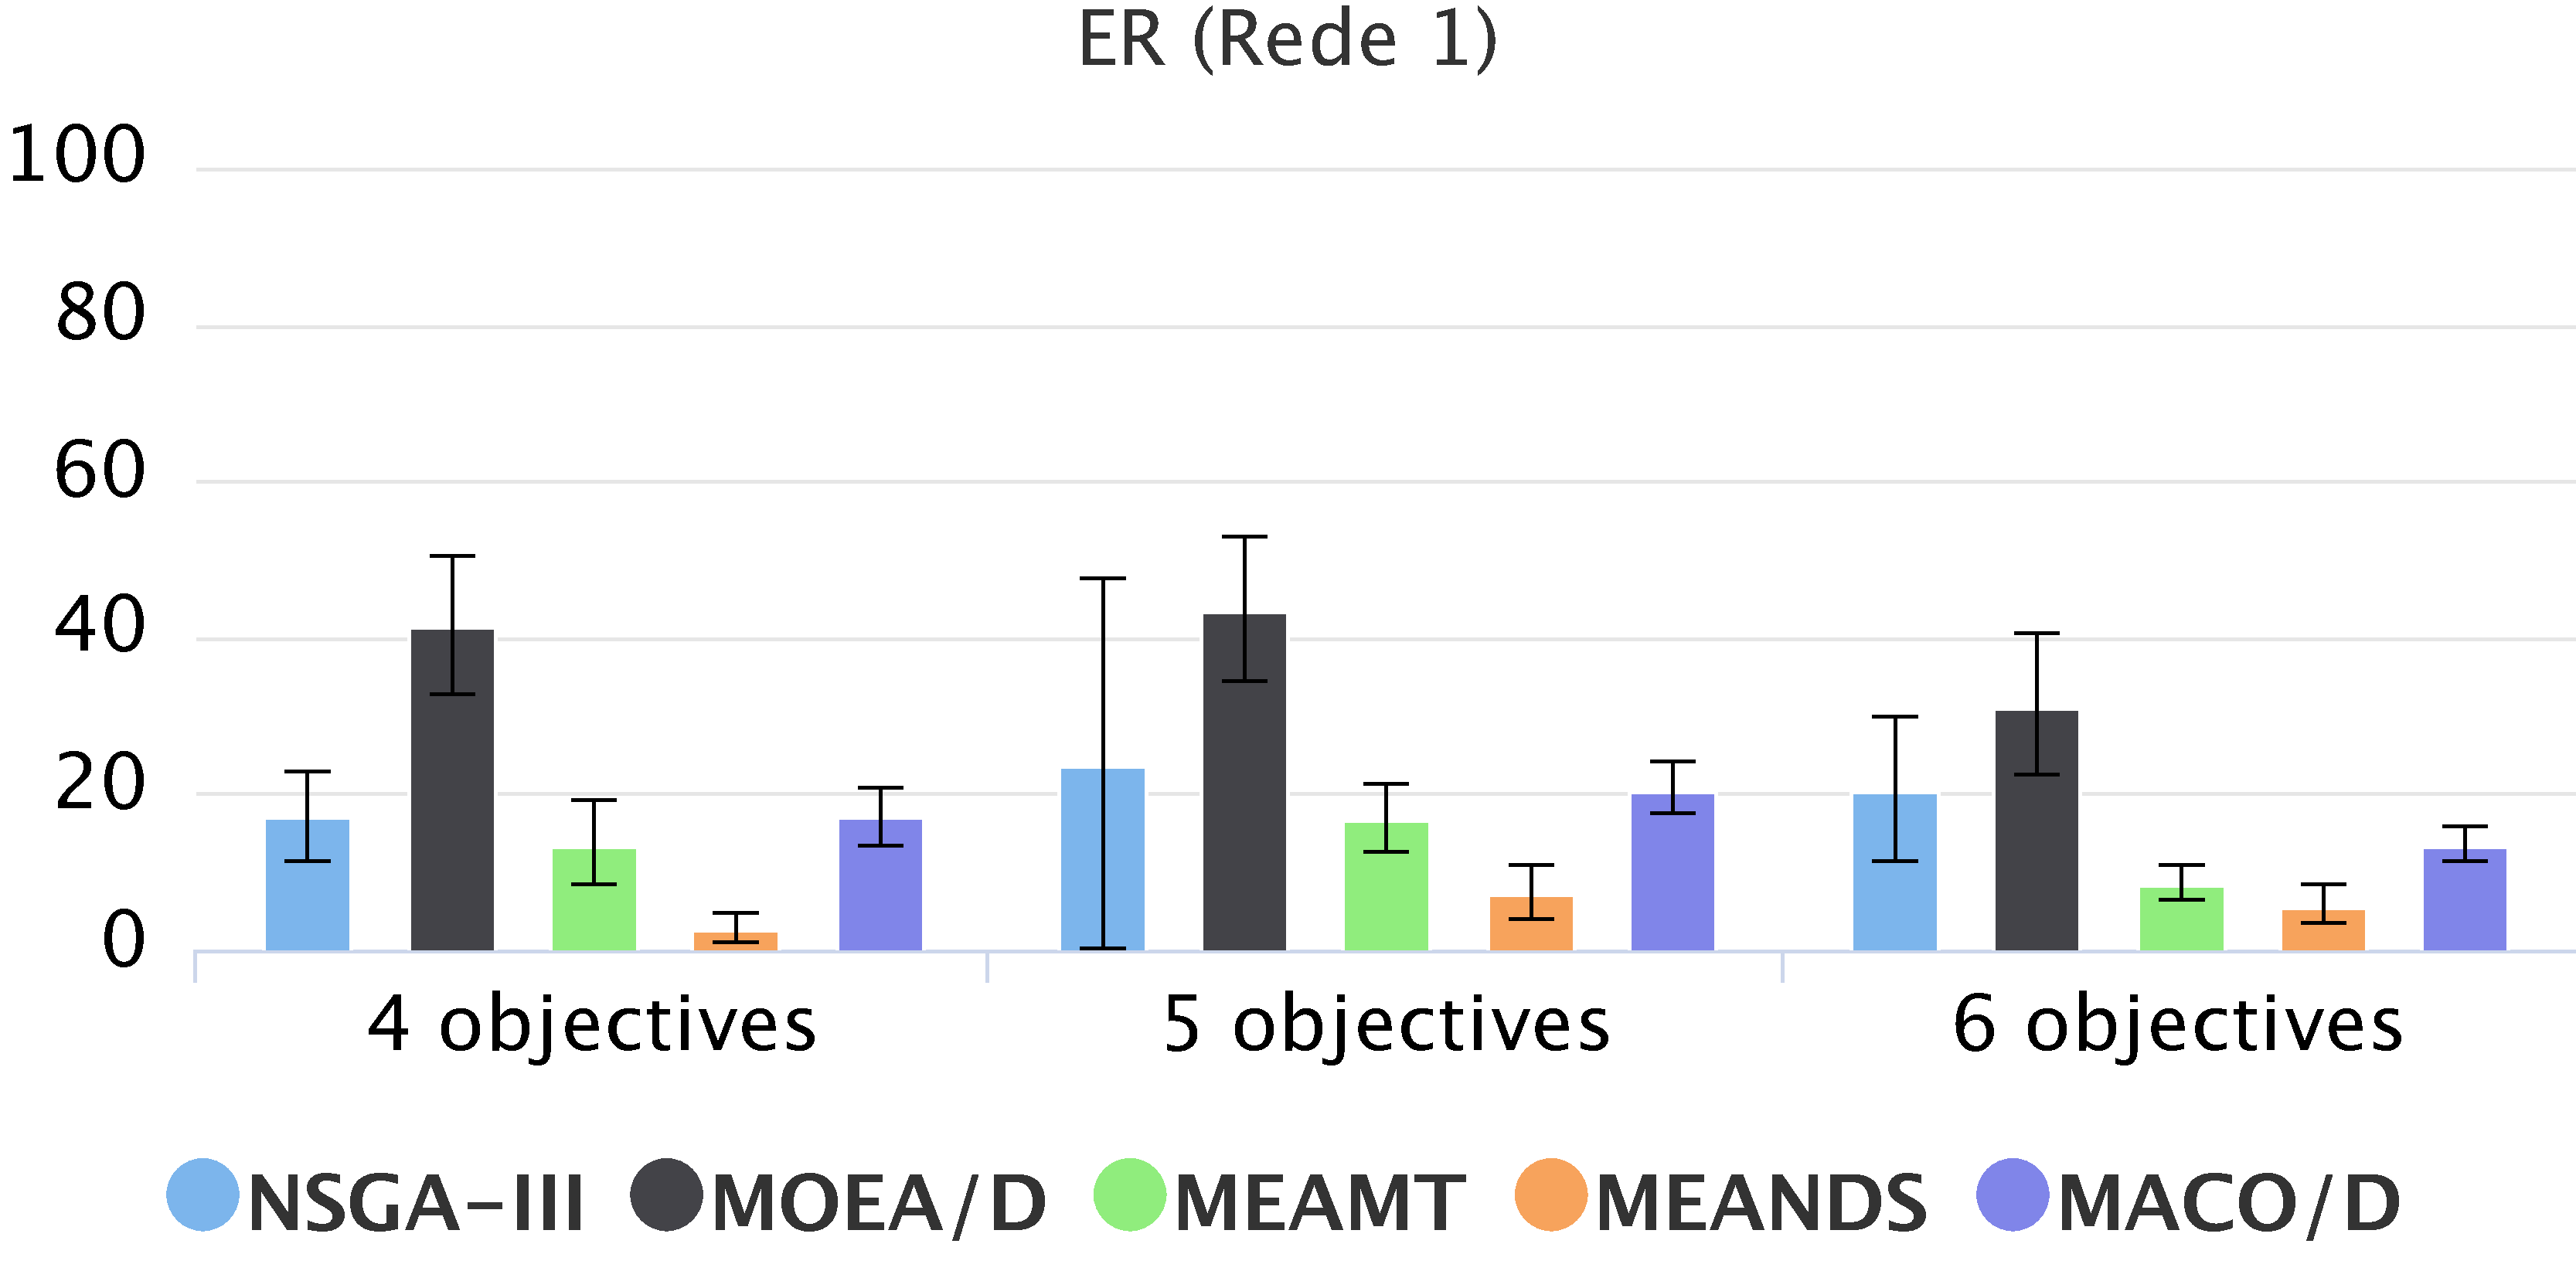
\includegraphics[width=0.5\textwidth]{cap_experimentos/figs/etapa2/er-mrp-r1}
	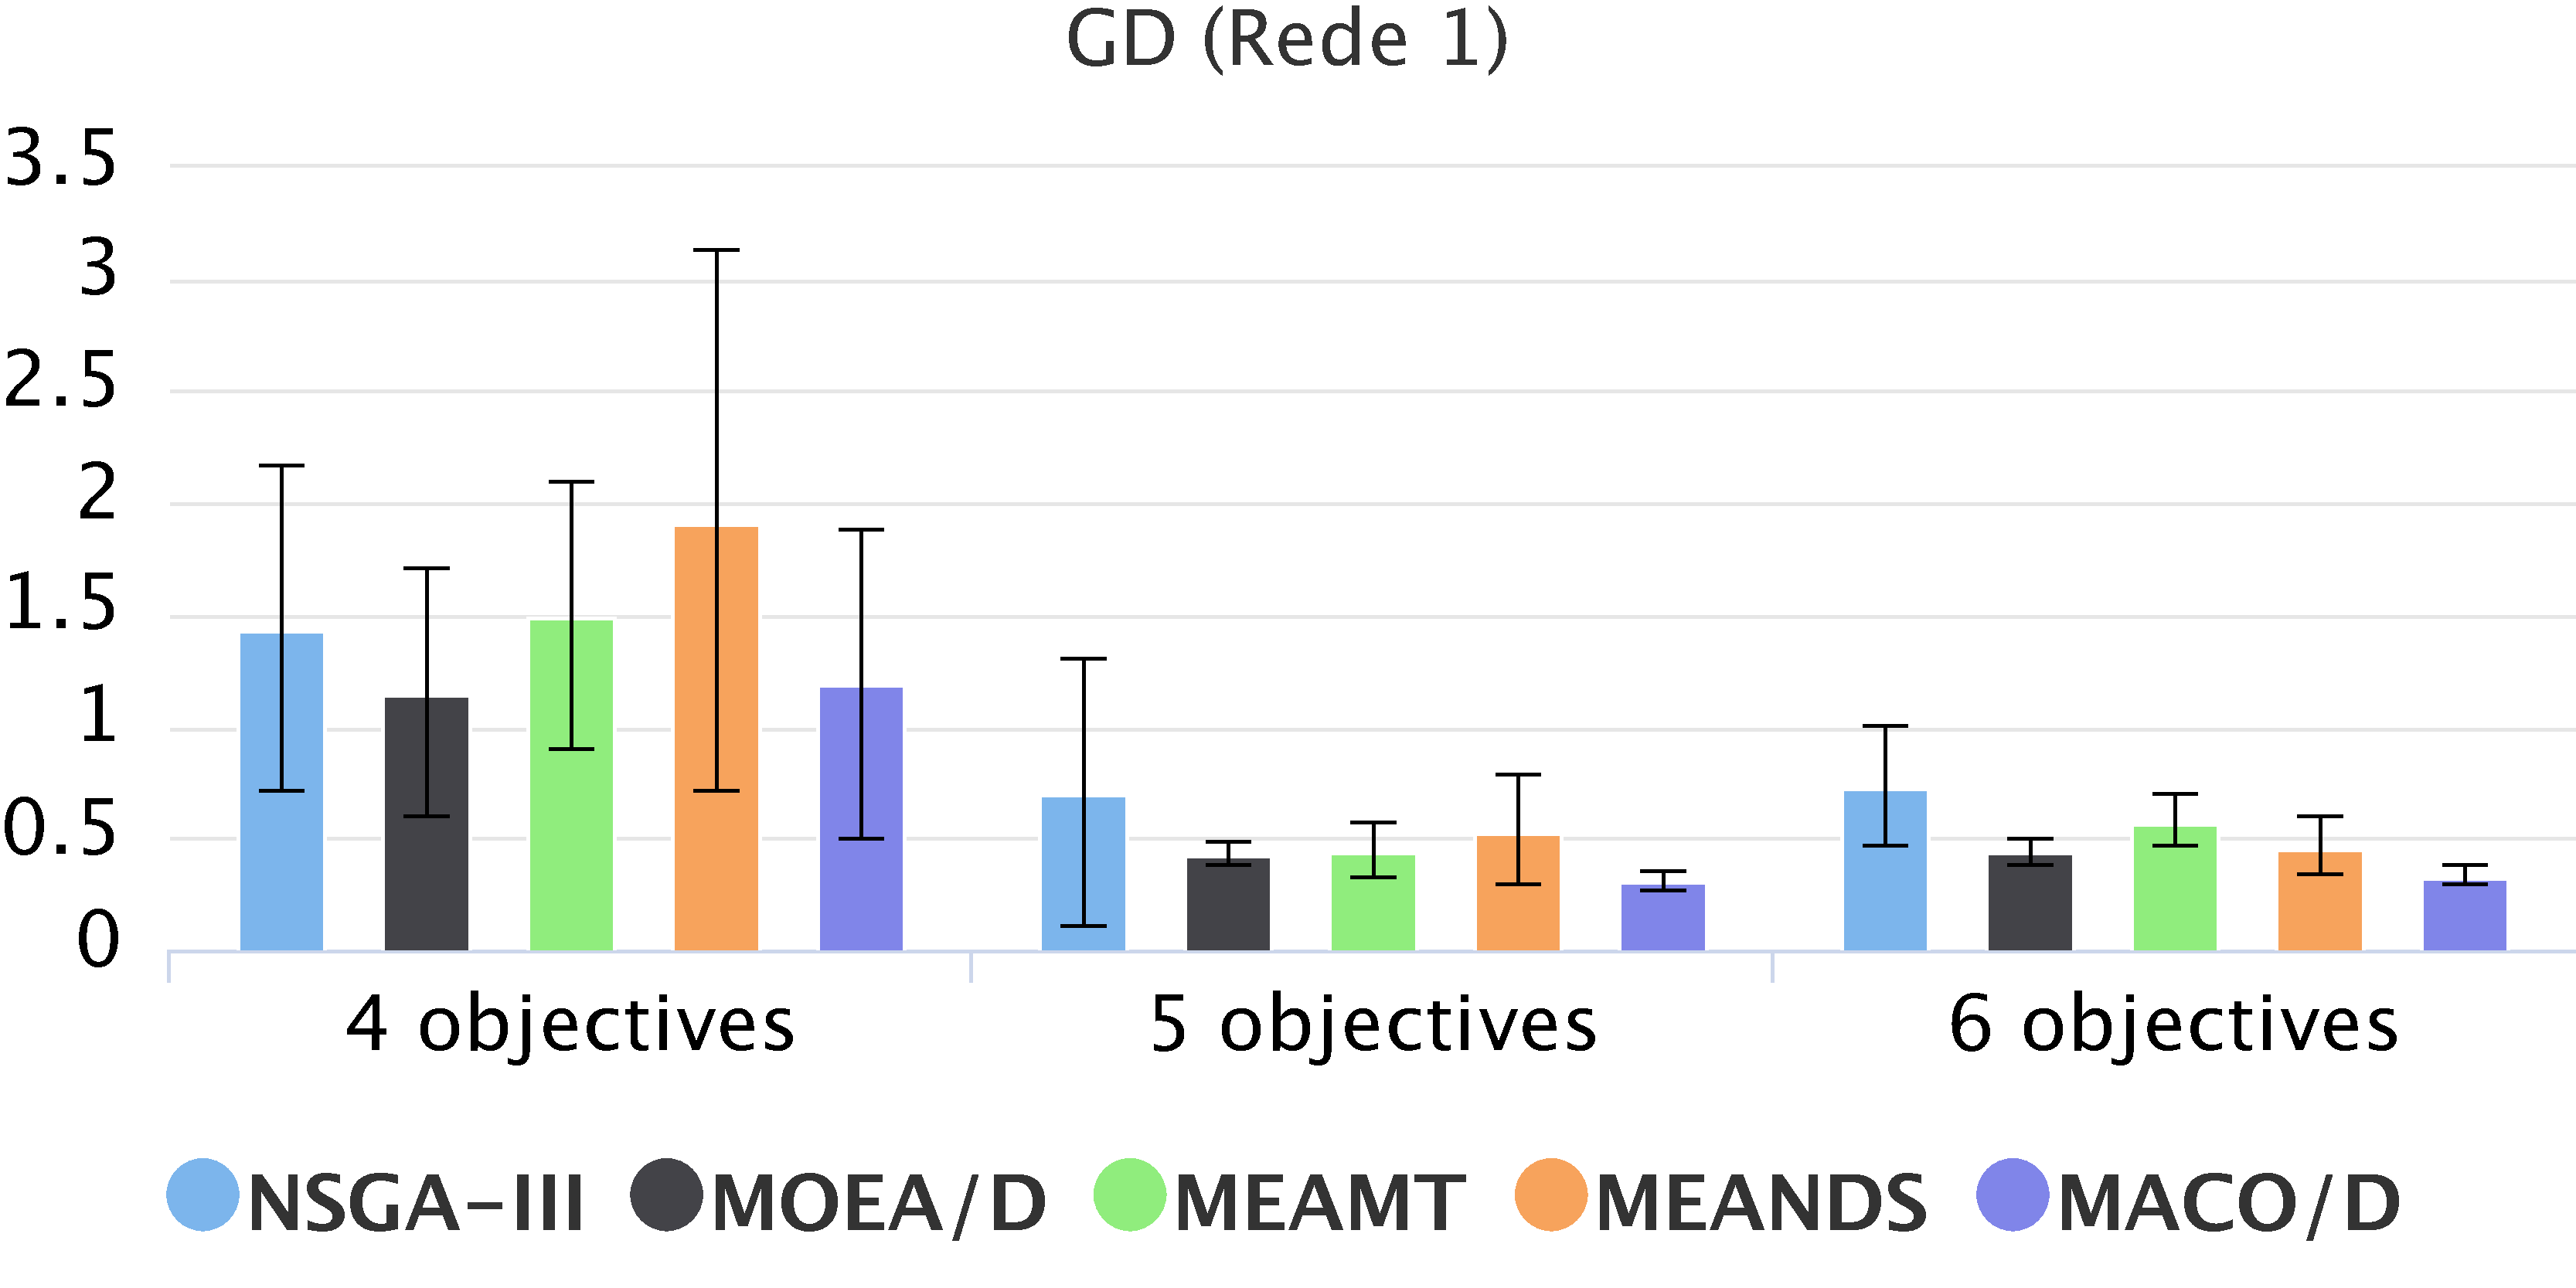
\includegraphics[width=0.5\textwidth]{cap_experimentos/figs/etapa2/gd-mrp-r1}
	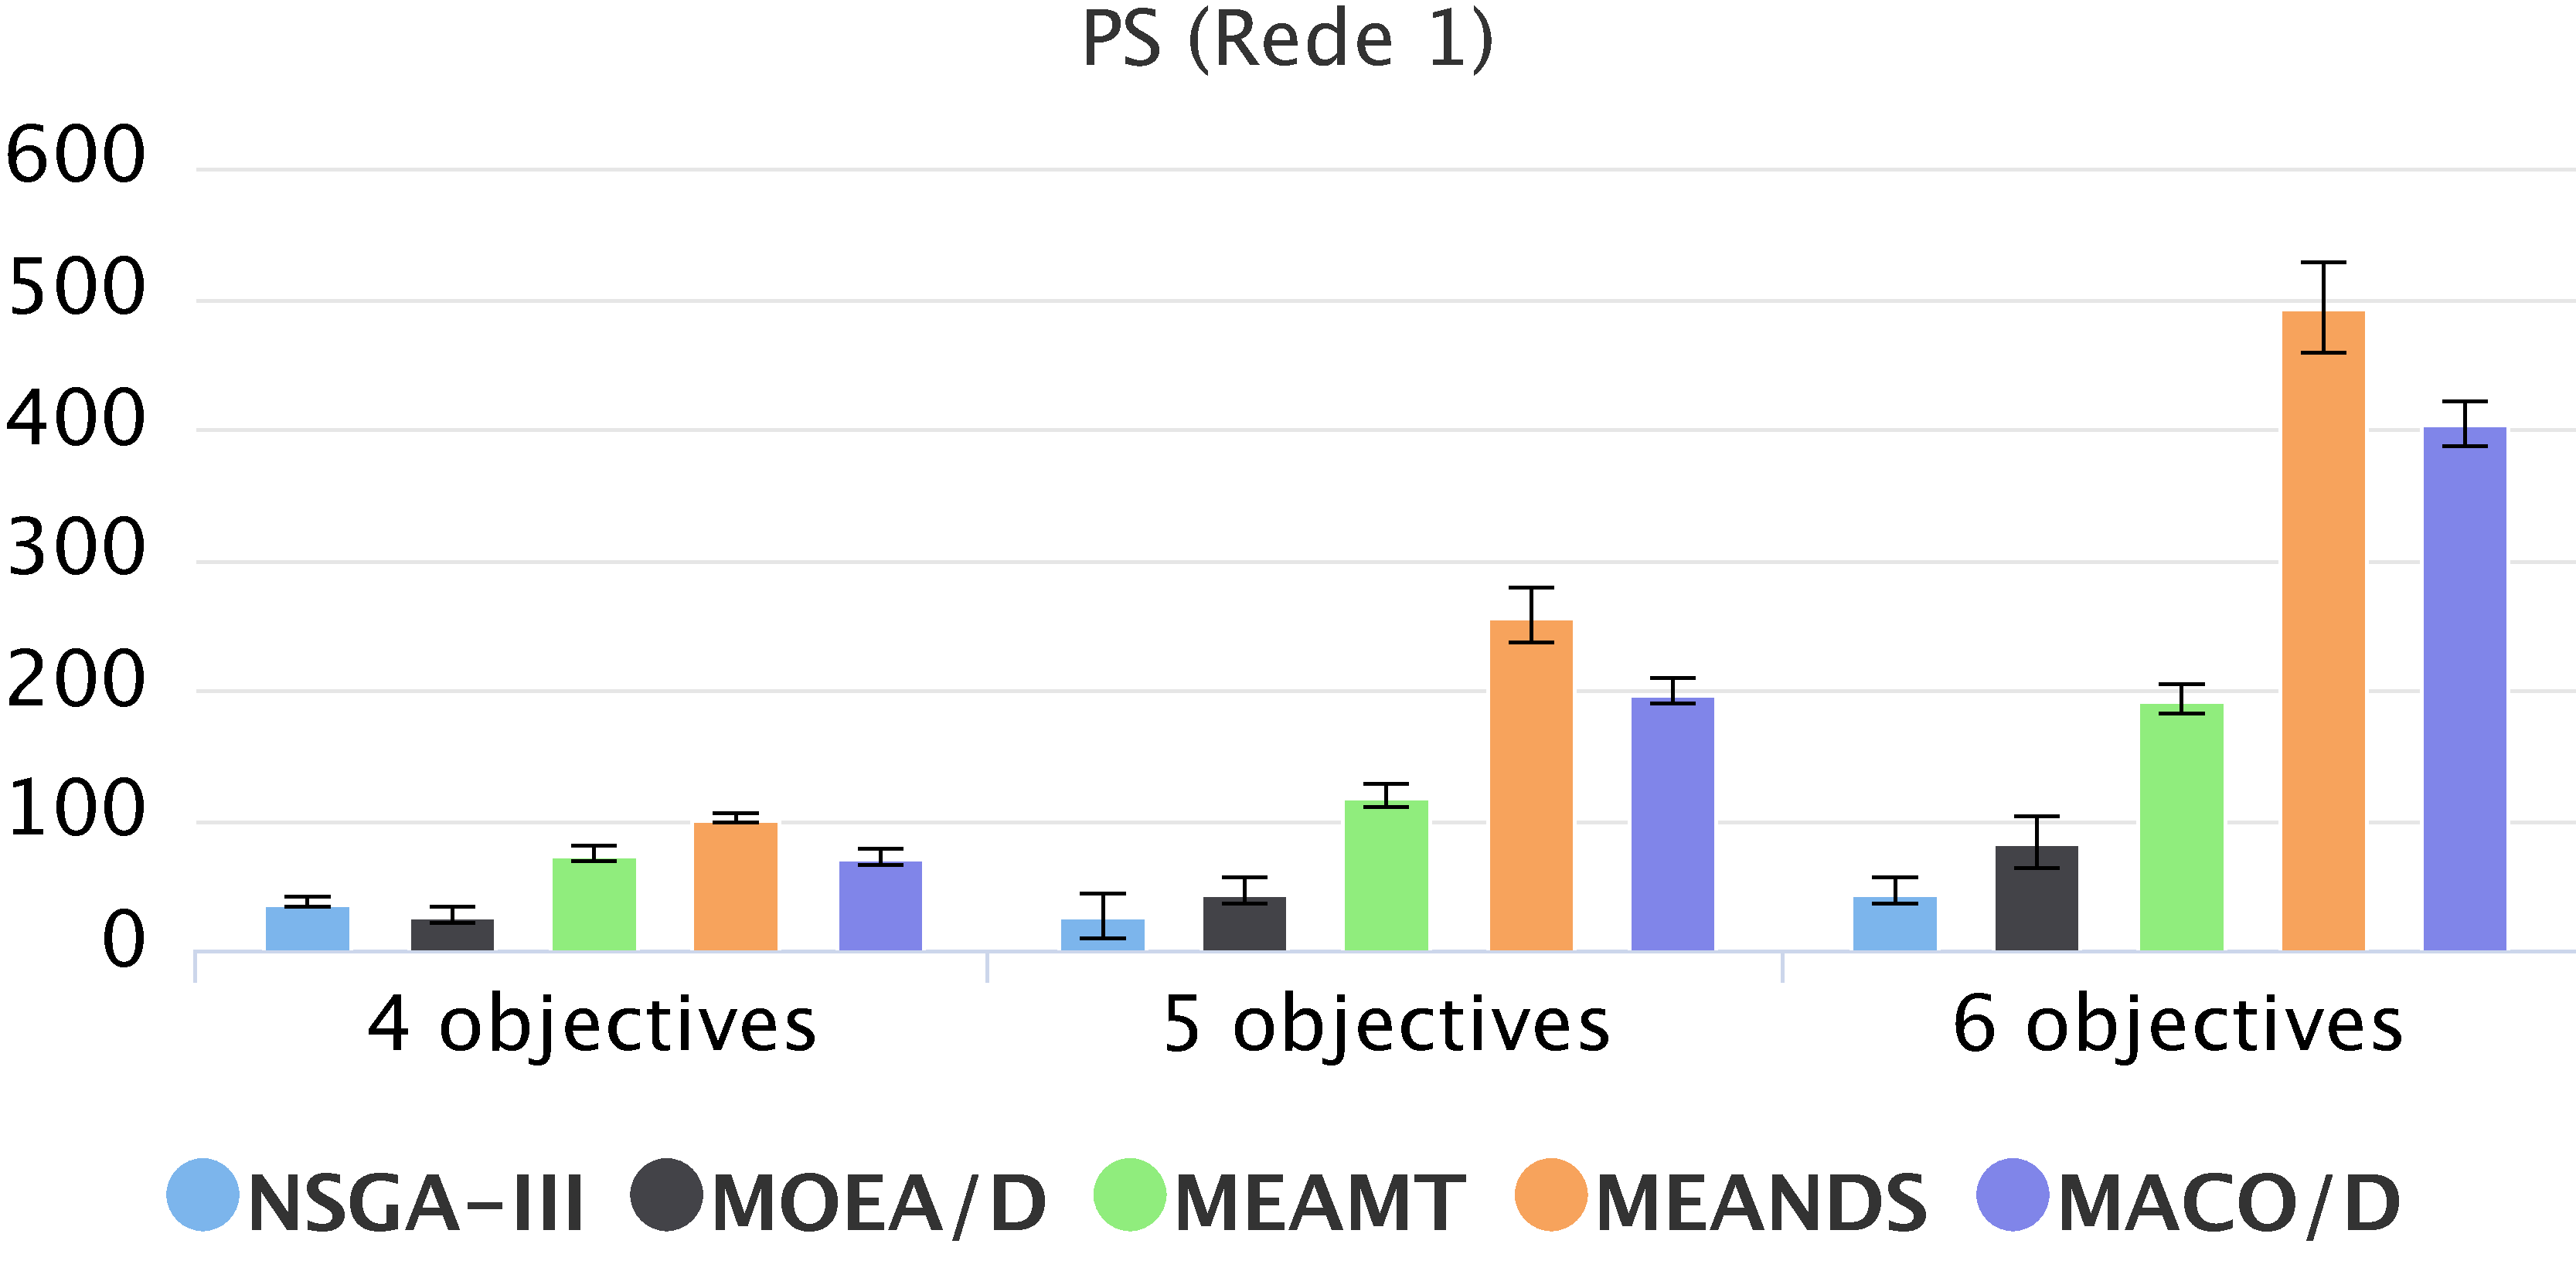
\includegraphics[width=0.5\textwidth]{cap_experimentos/figs/etapa2/ps-mrp-r1}
	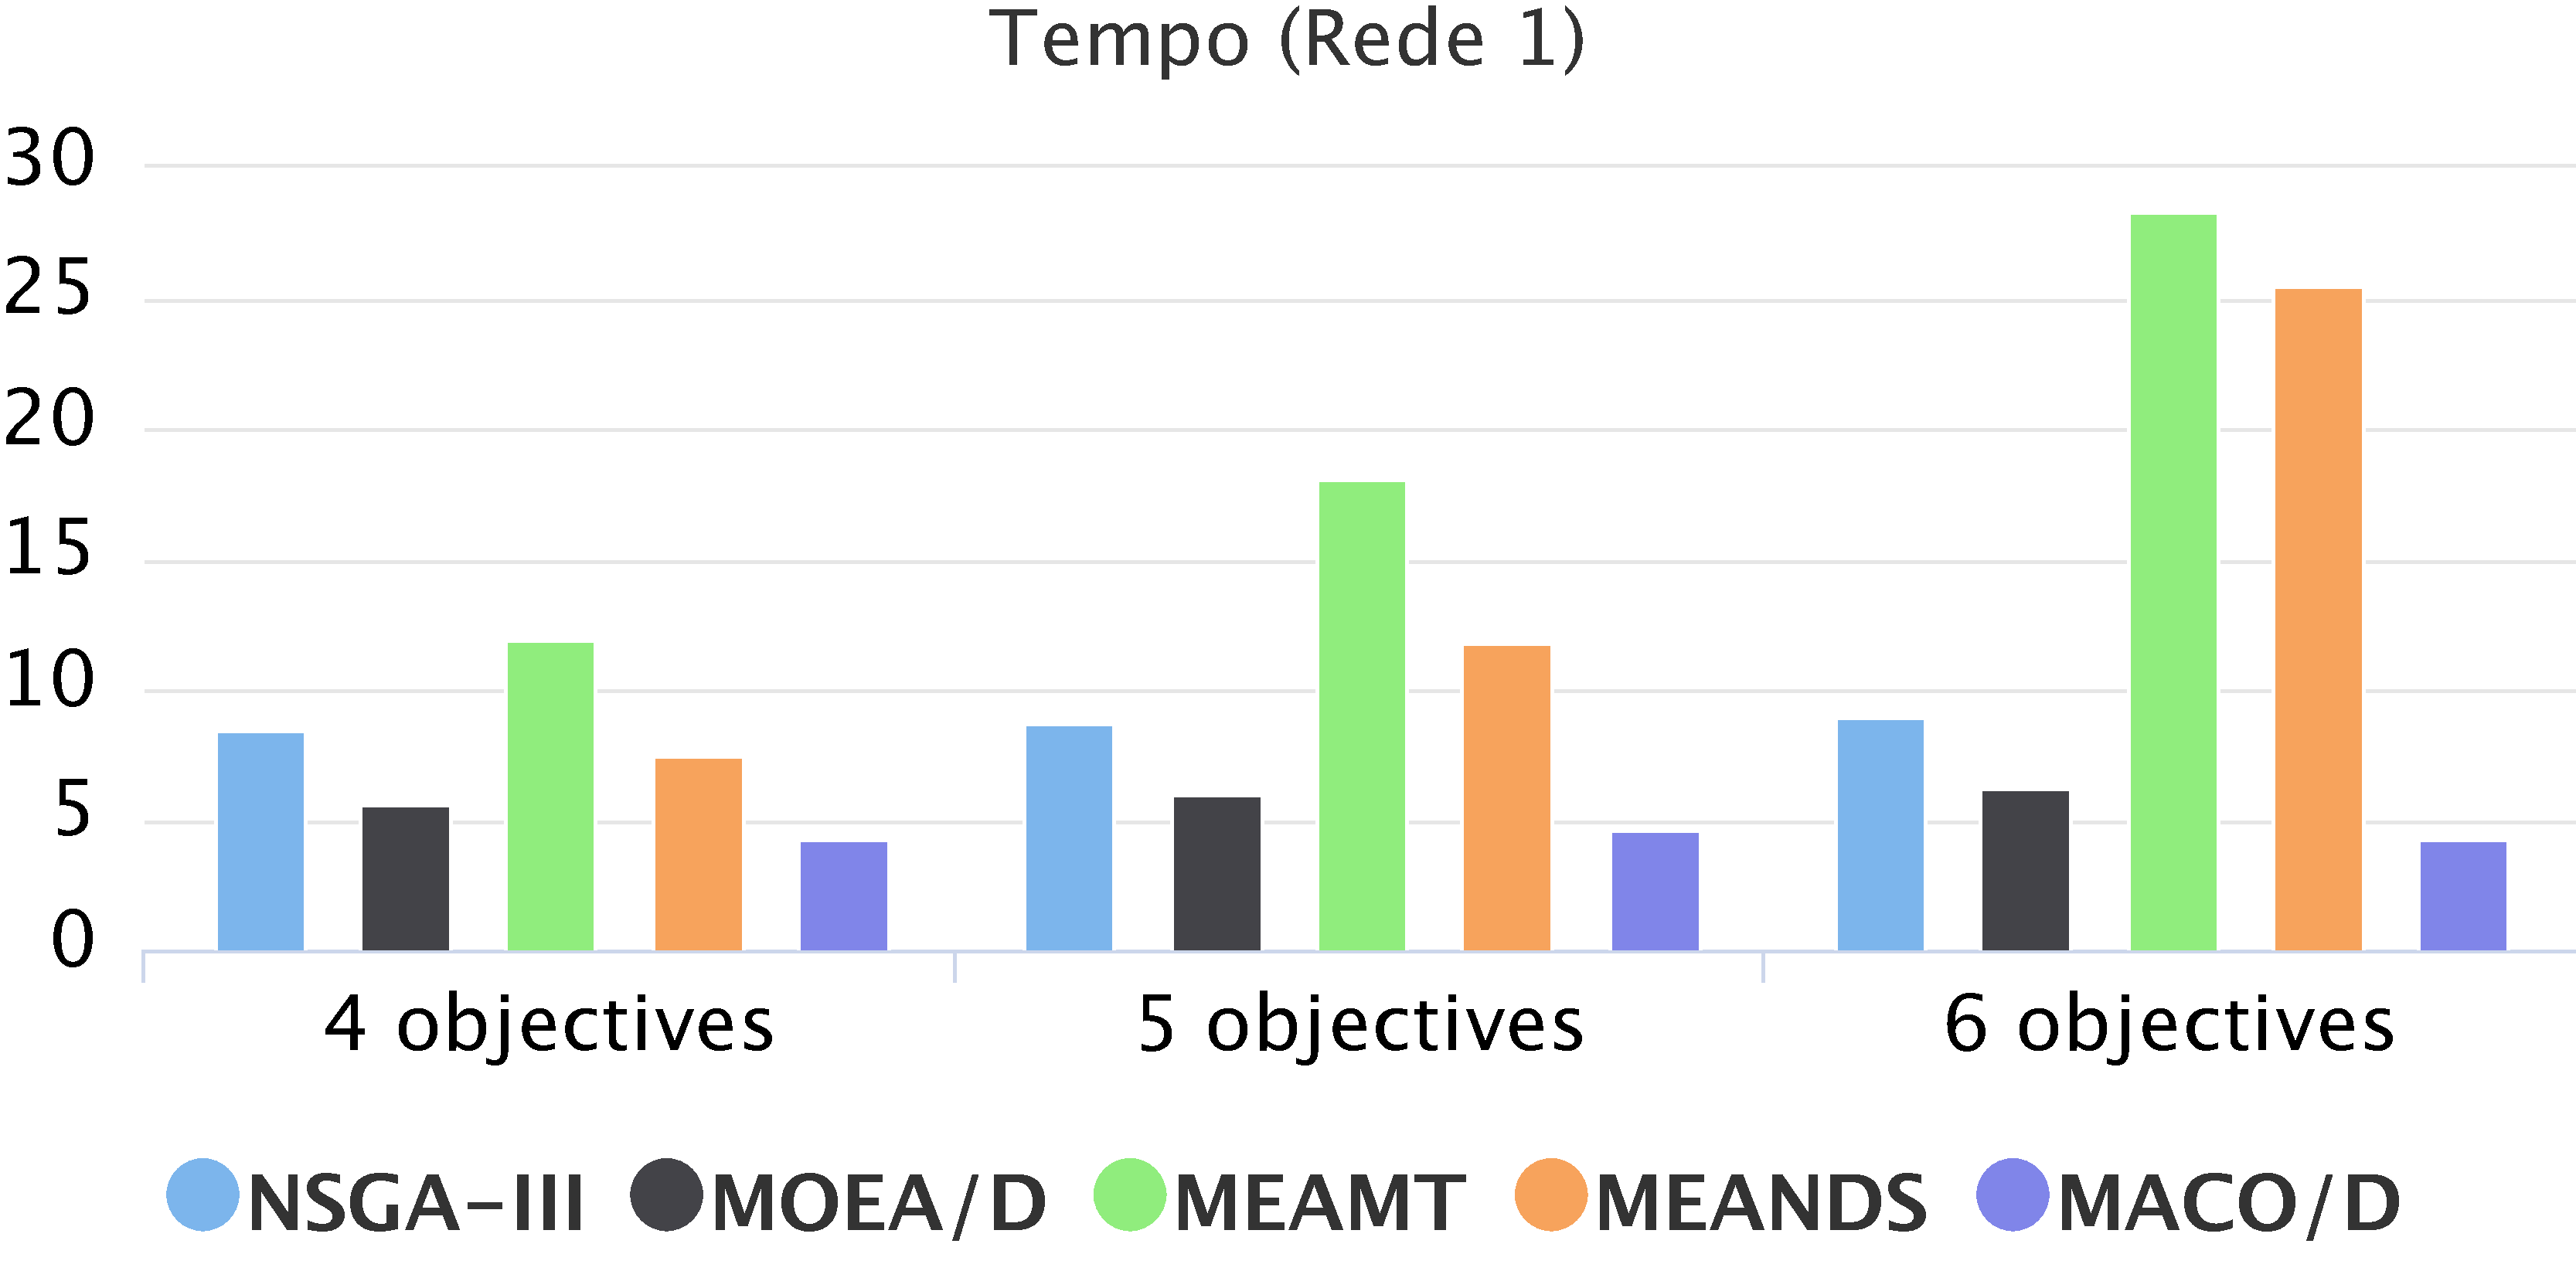
\includegraphics[width=0.5\textwidth]{cap_experimentos/figs/etapa2/time-mrp-r1}
\end{figure*}

Análise do PRM-R1

\begin{figure*}[!htbp]
	\caption{Etapa 2: resultados para o PRM na rede $R_2$}
	\label{fig_exp2_mrp_r2}
	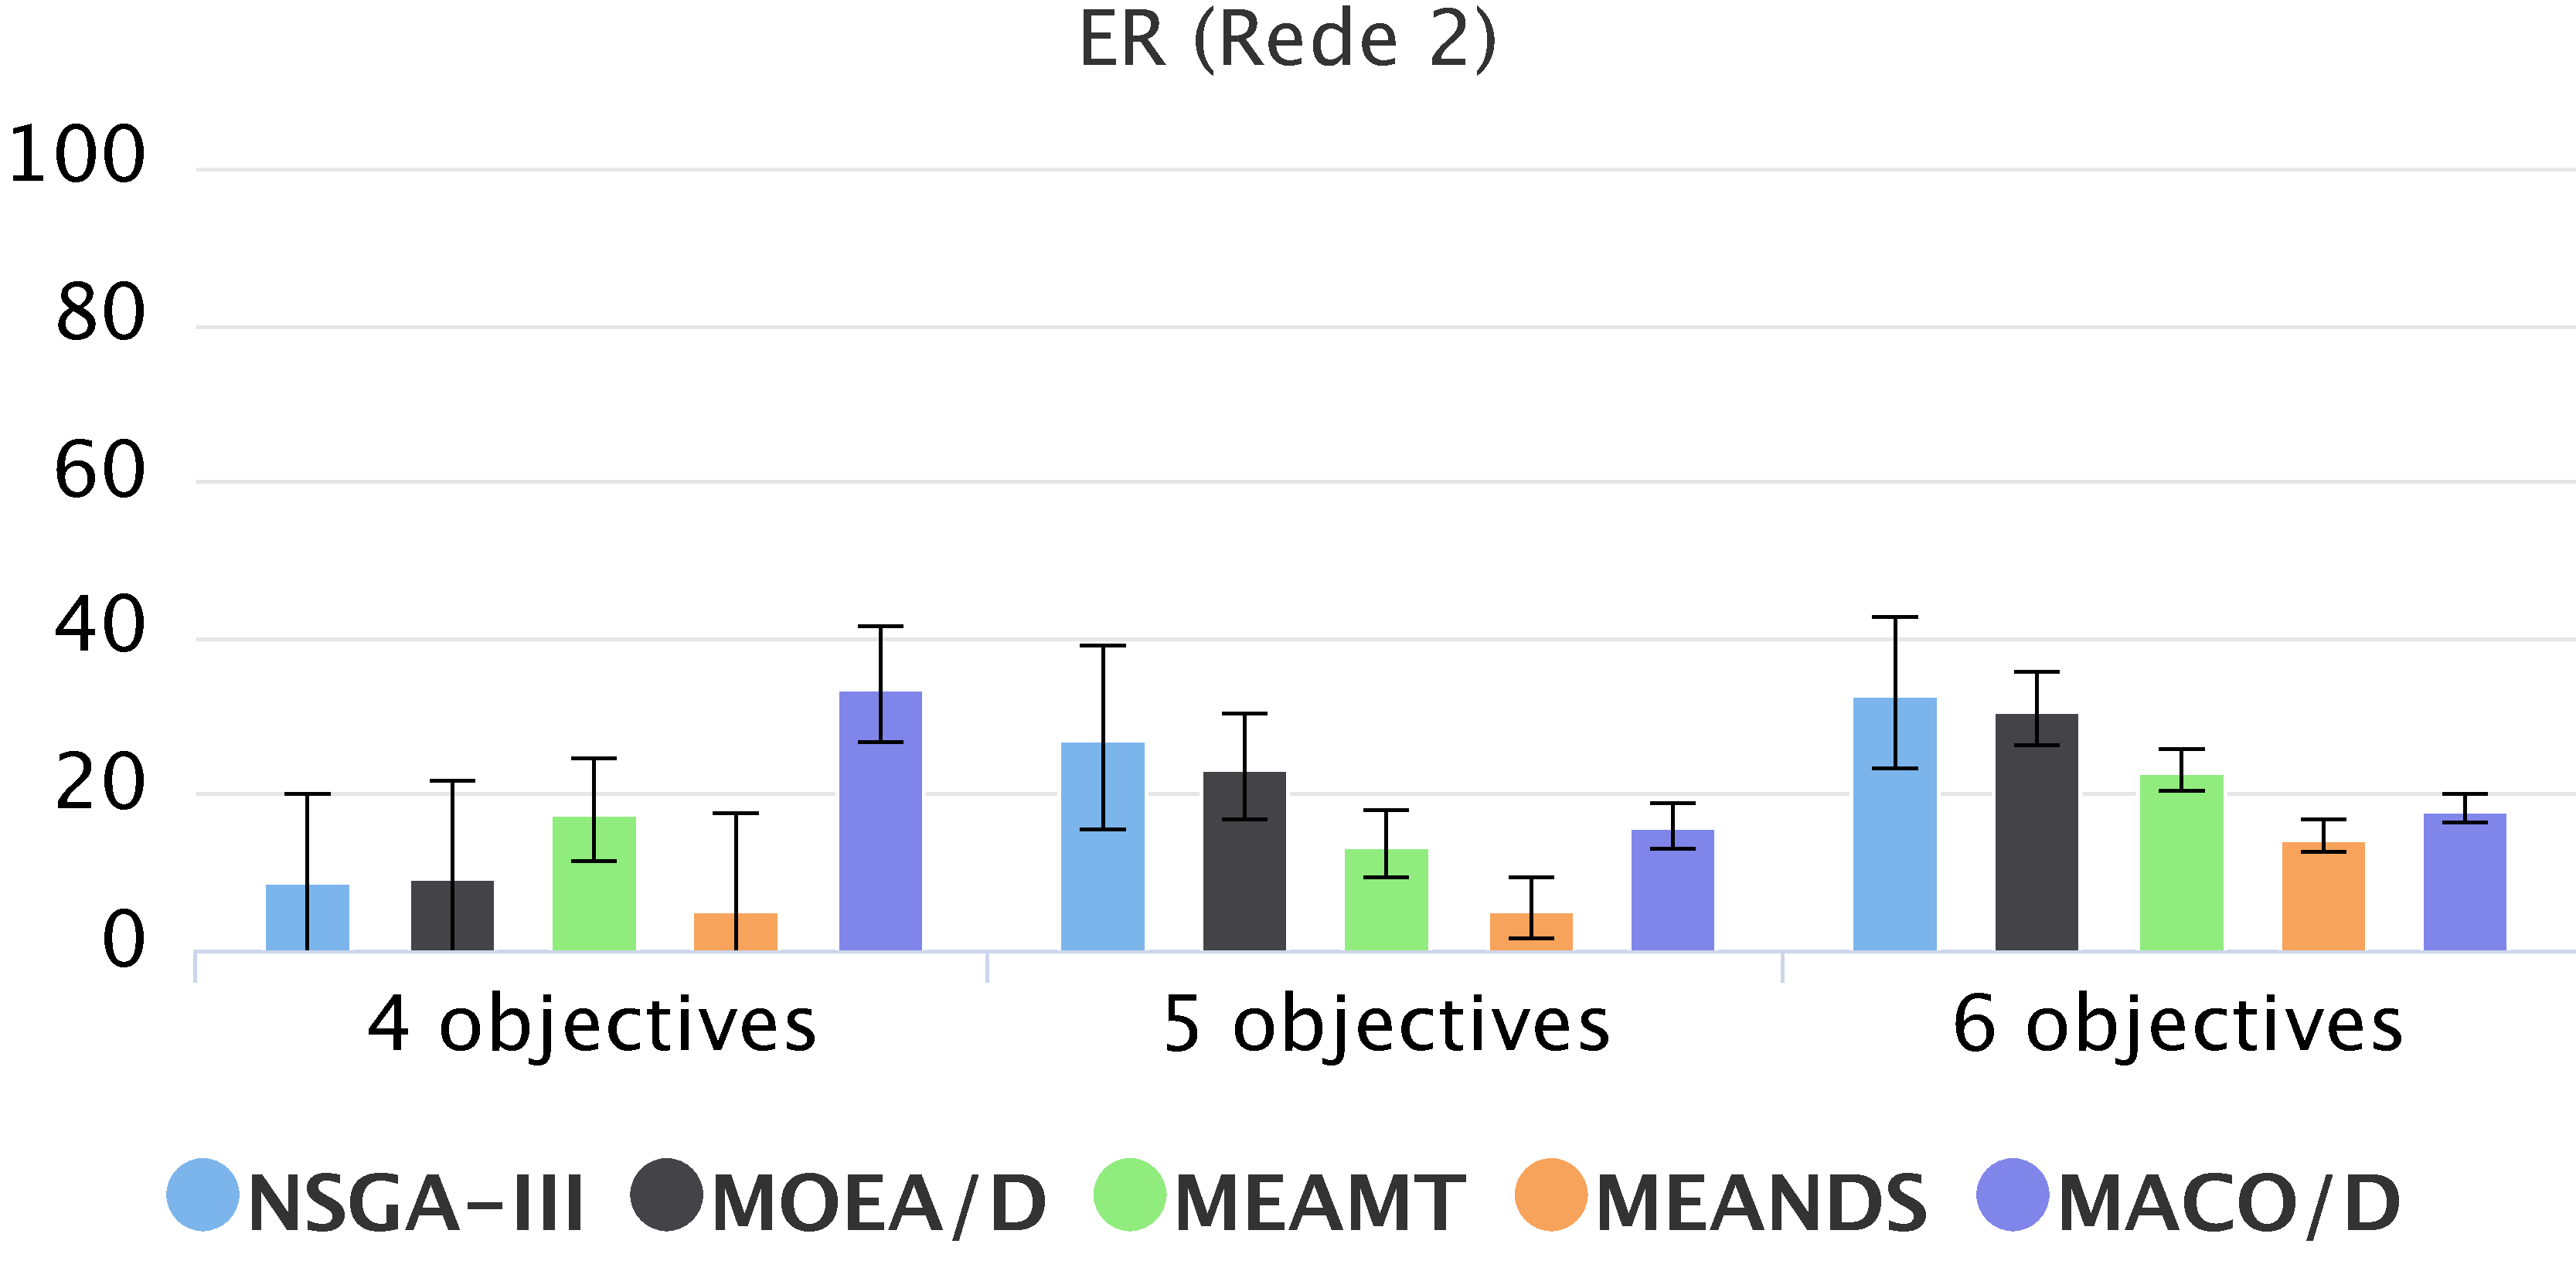
\includegraphics[width=0.5\textwidth]{cap_experimentos/figs/etapa2/er-mrp-r2}
	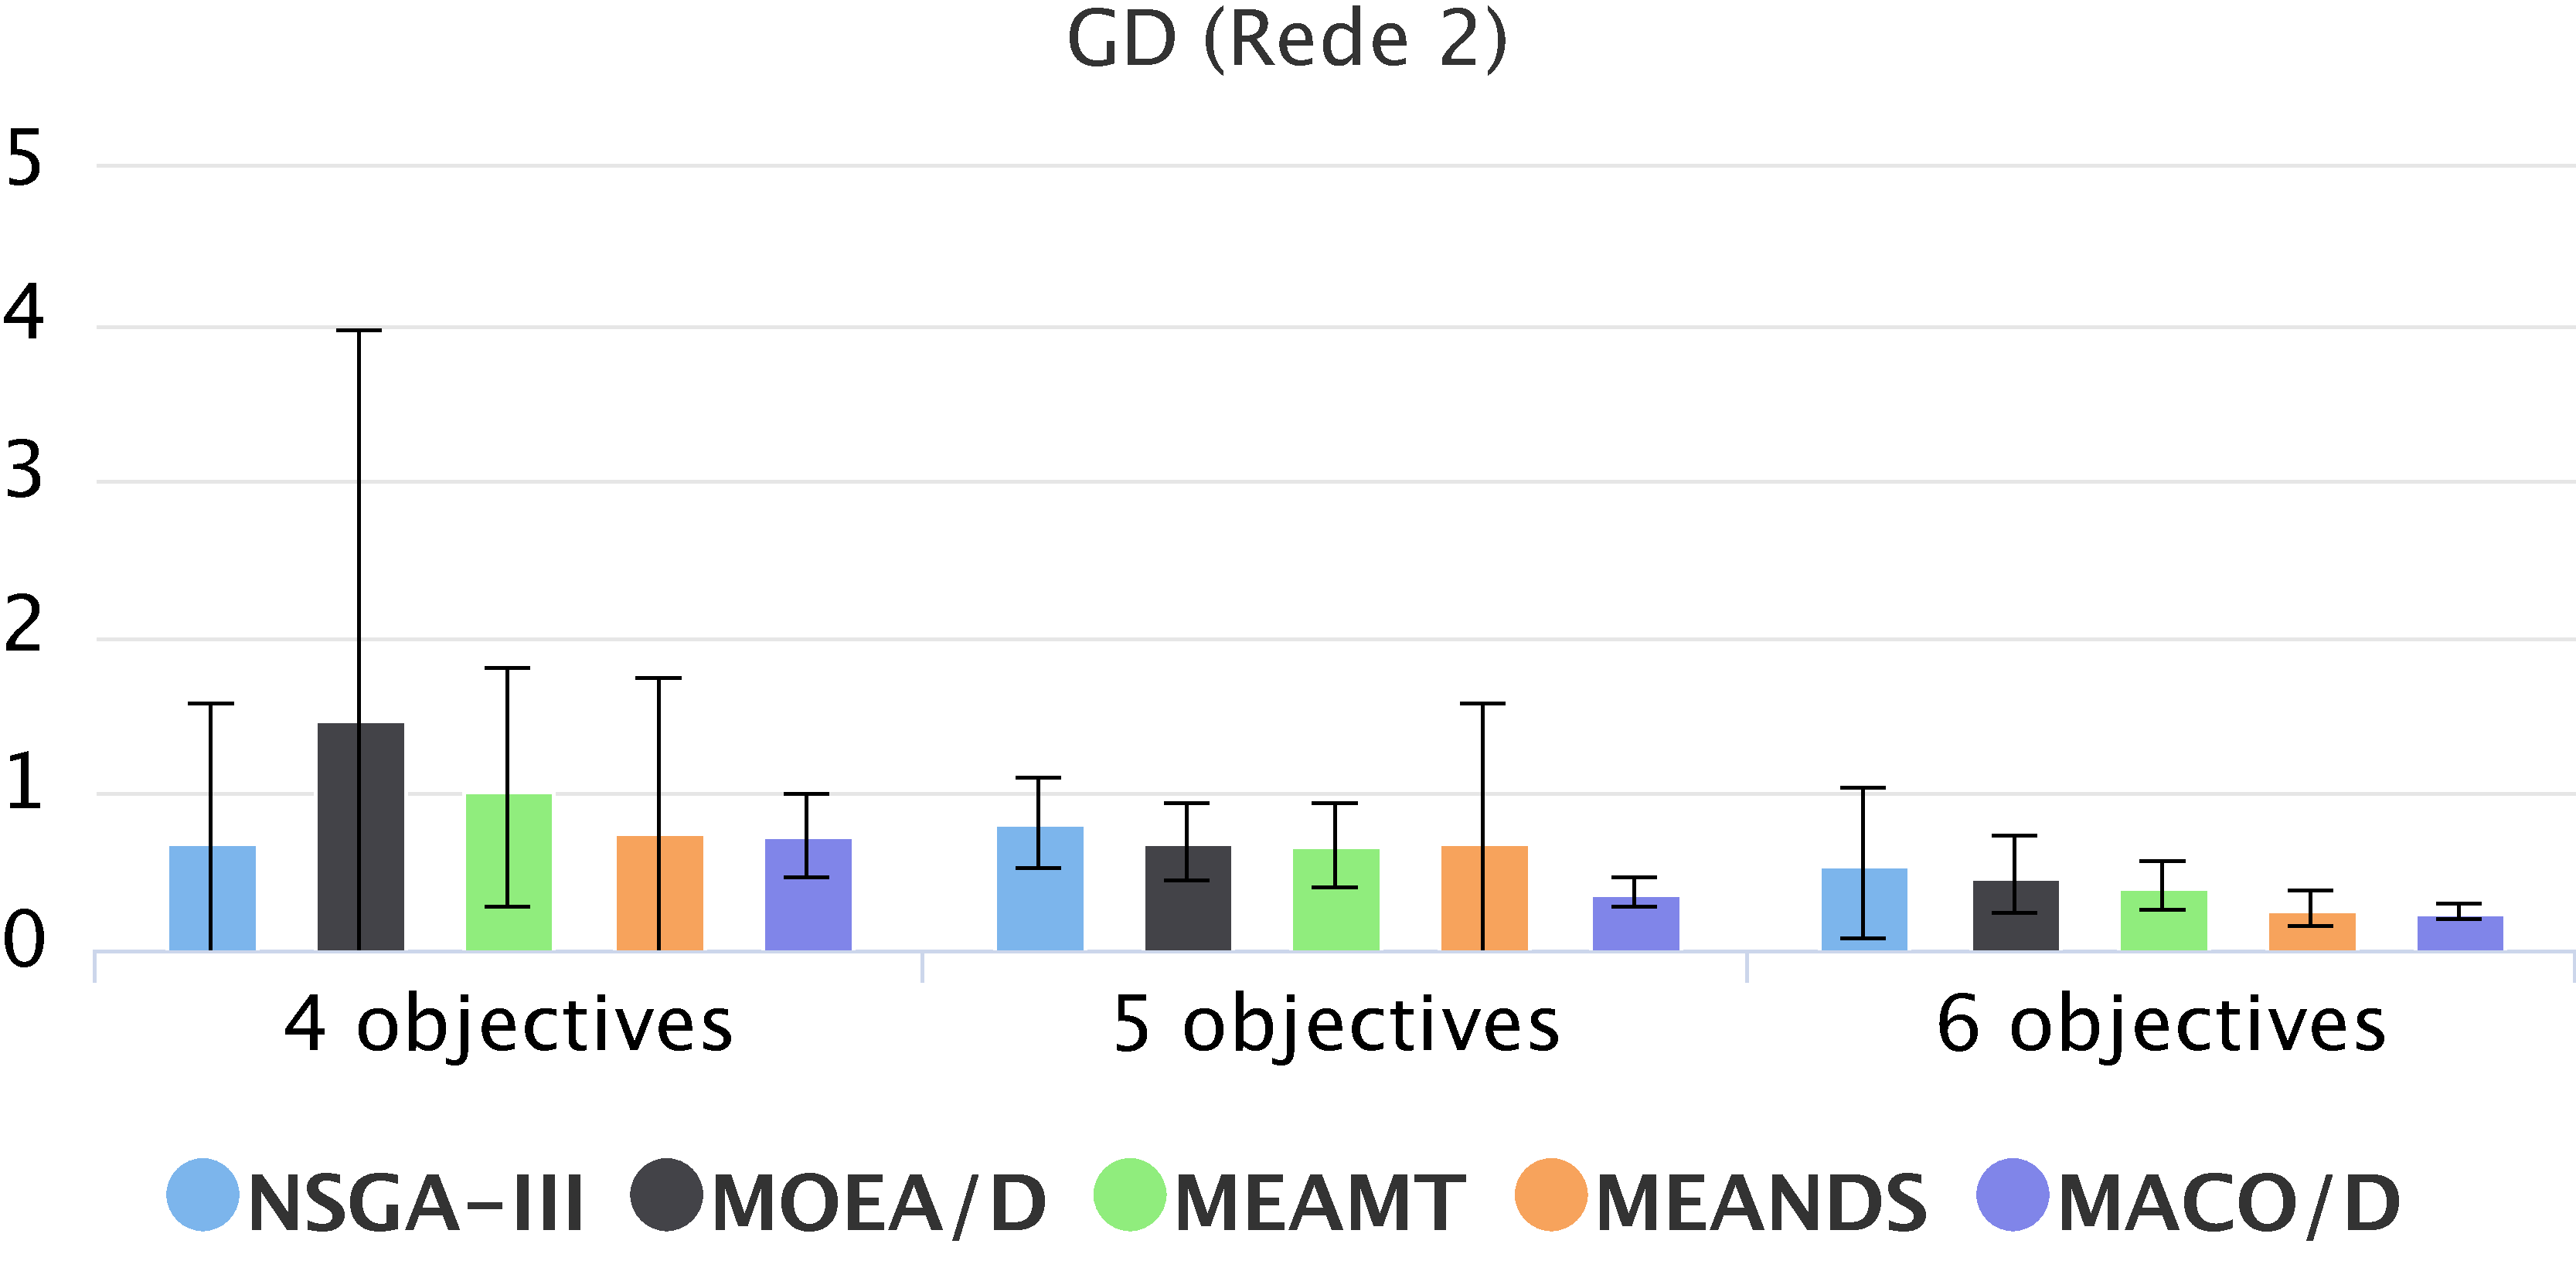
\includegraphics[width=0.5\textwidth]{cap_experimentos/figs/etapa2/gd-mrp-r2}
	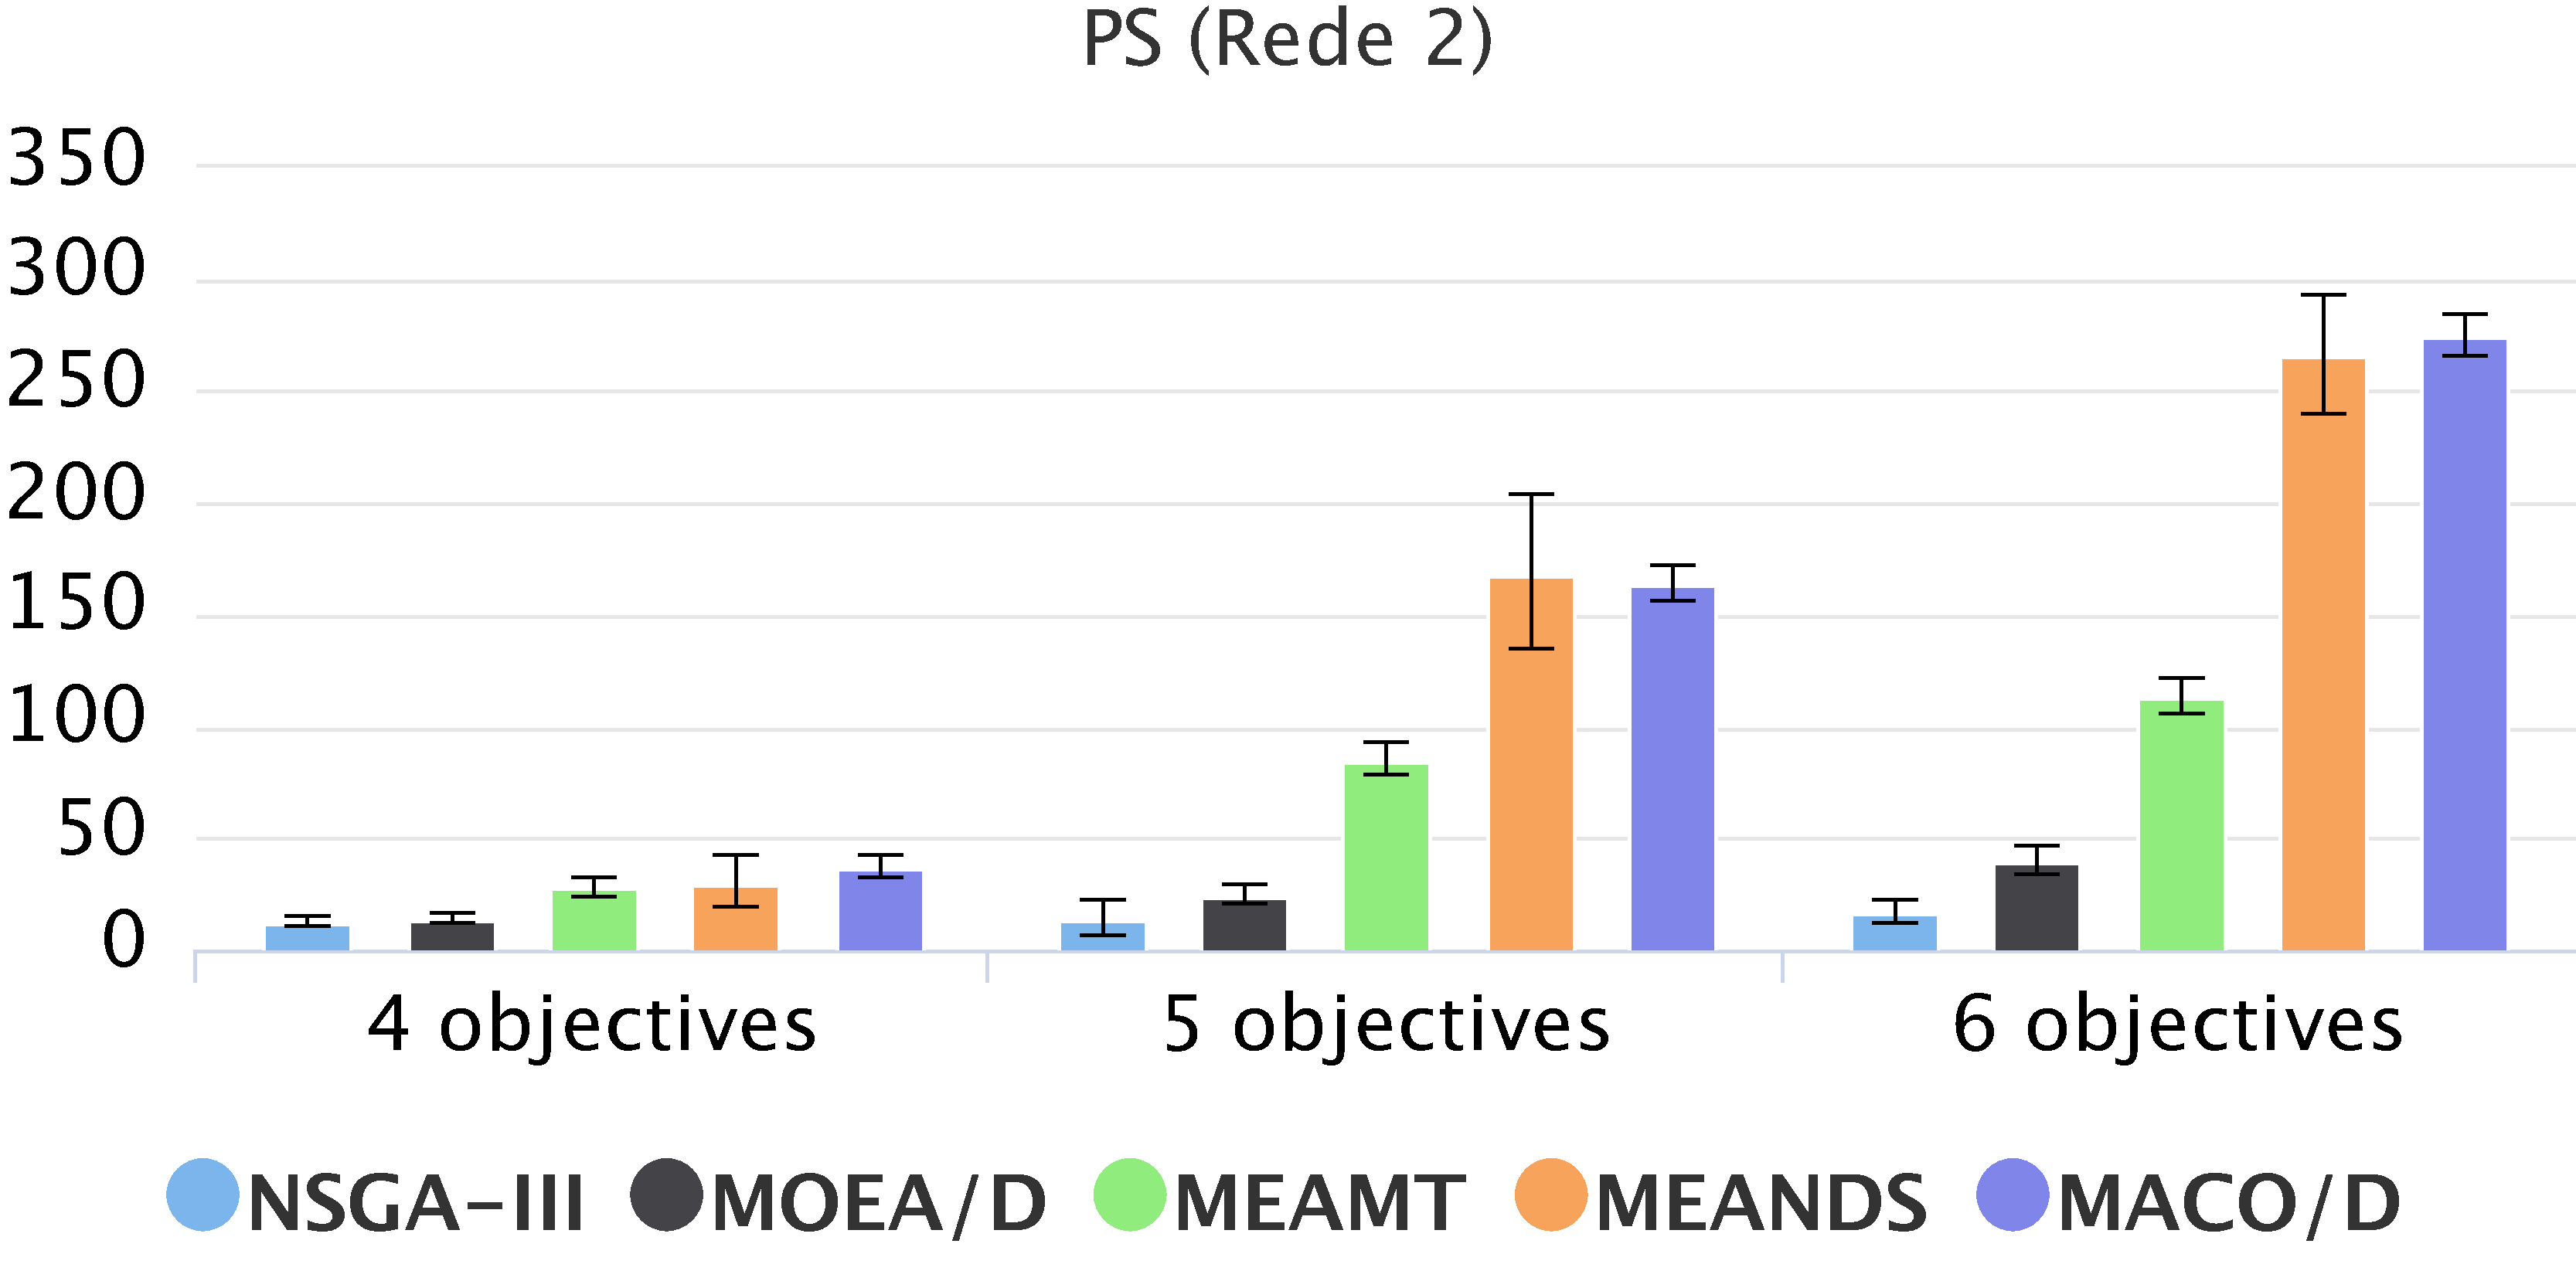
\includegraphics[width=0.5\textwidth]{cap_experimentos/figs/etapa2/ps-mrp-r2}
	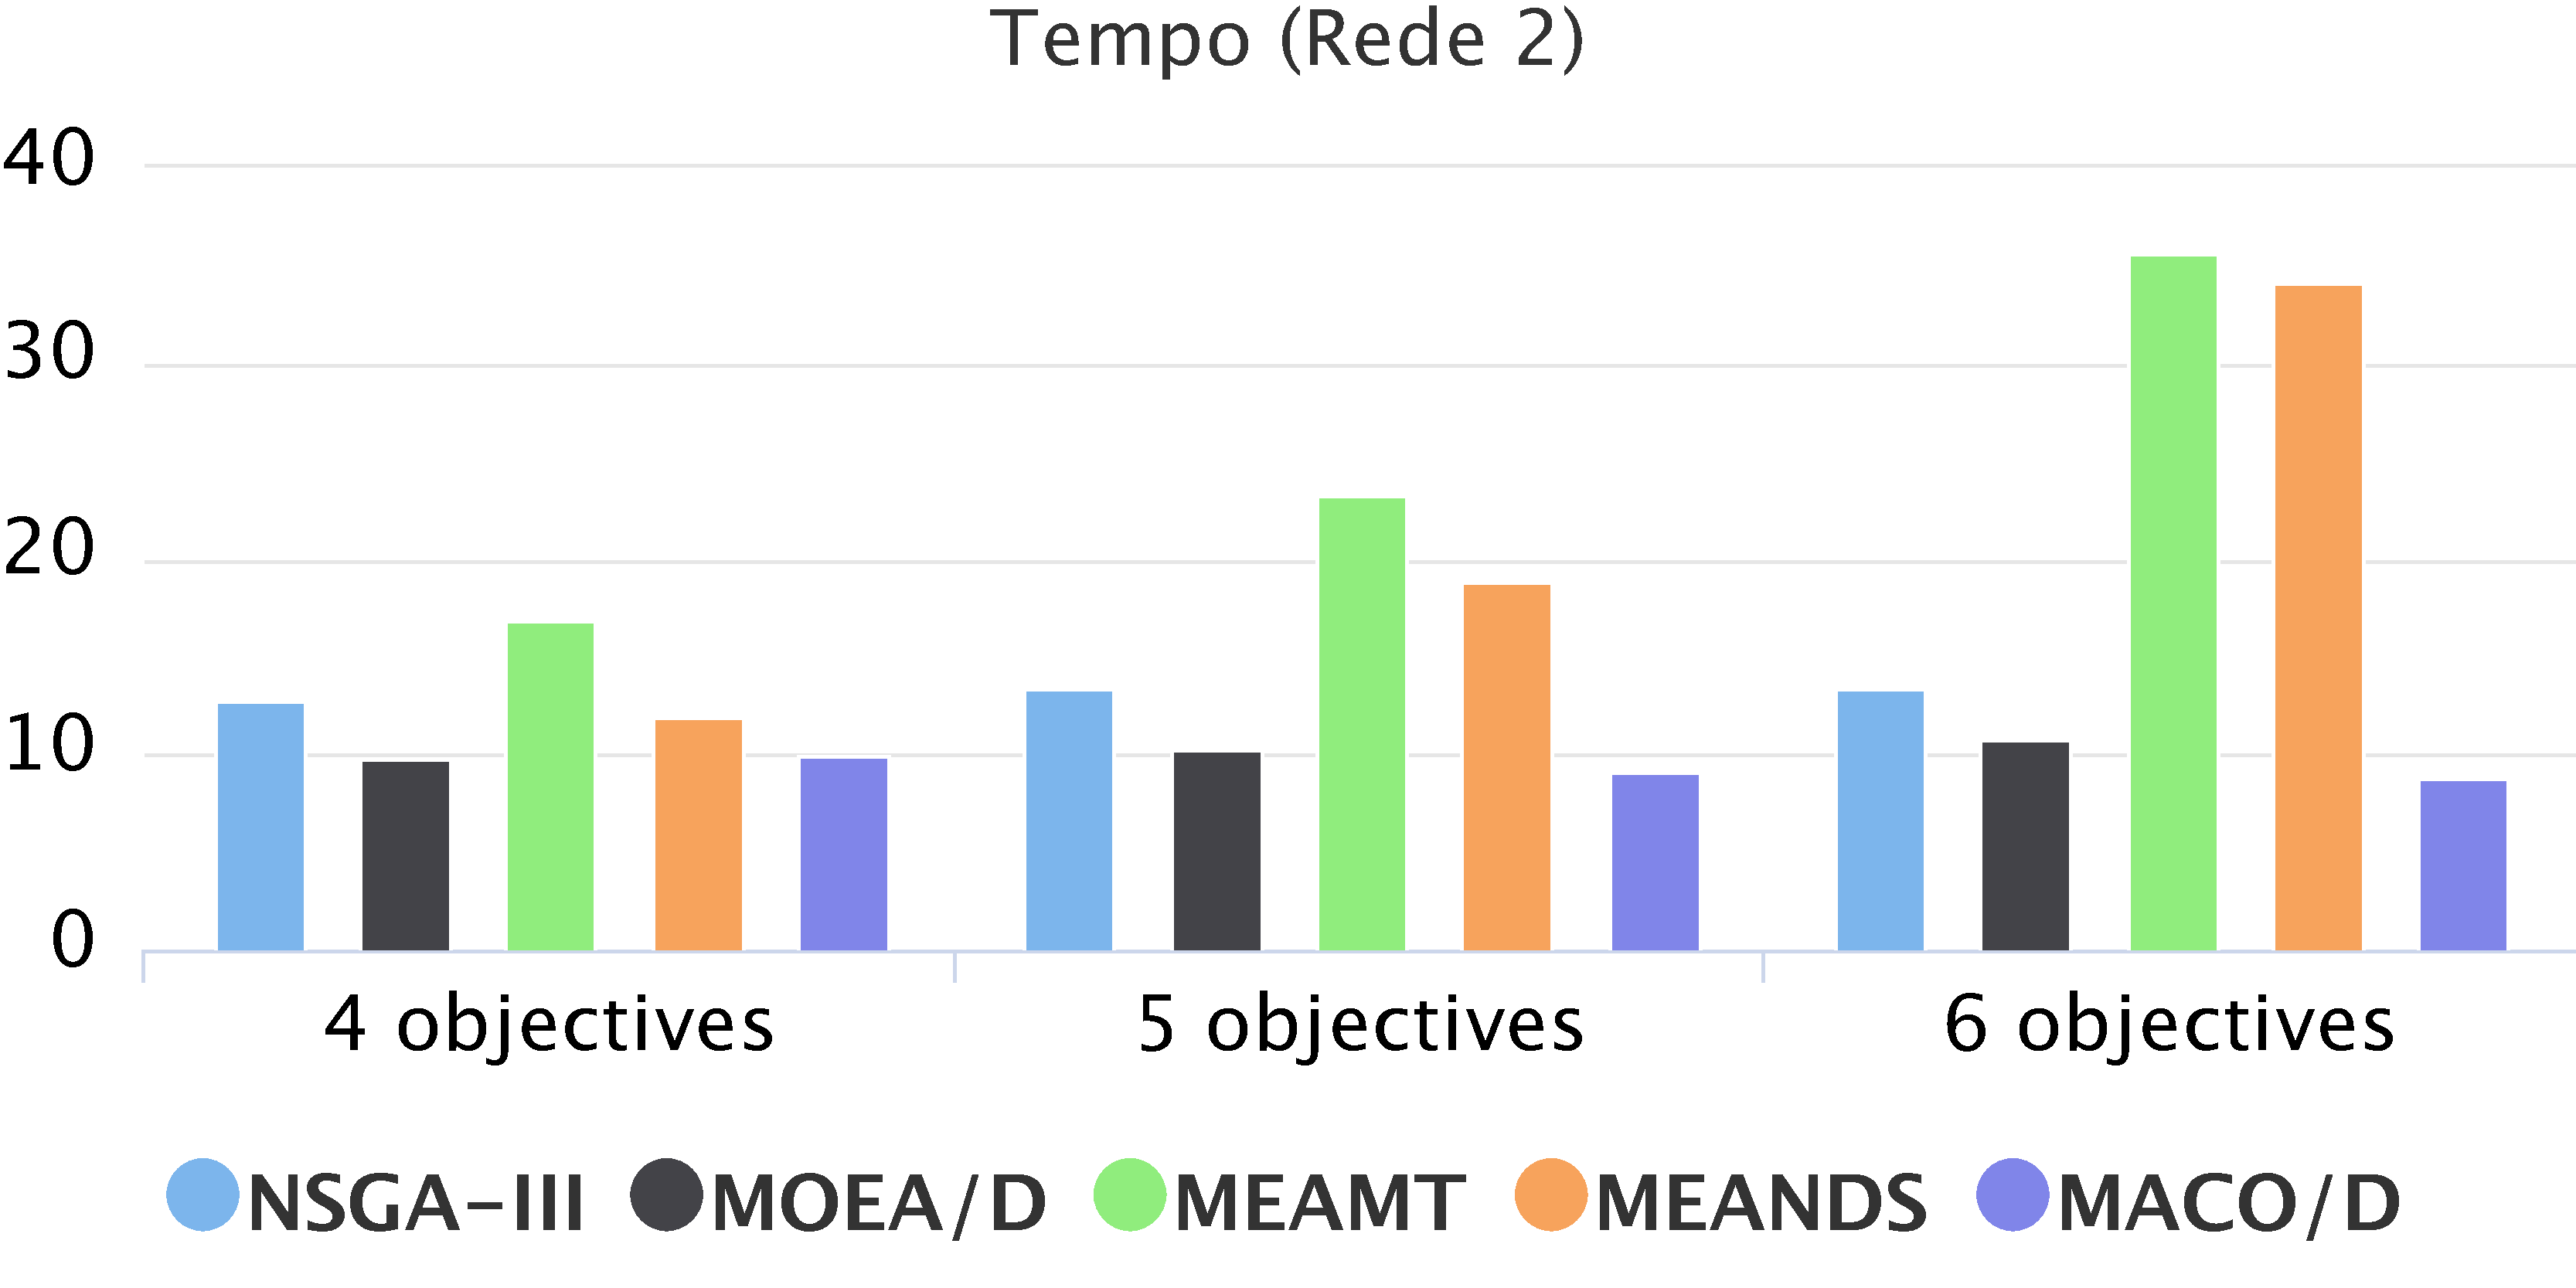
\includegraphics[width=0.5\textwidth]{cap_experimentos/figs/etapa2/time-mrp-r2}
\end{figure*}

Análise do PRM-R2

\begin{figure*}[!htbp]
	\caption{Etapa 2: resultados para o PRM na rede $R_3$}
	\label{fig_exp2_mrp_r3}
	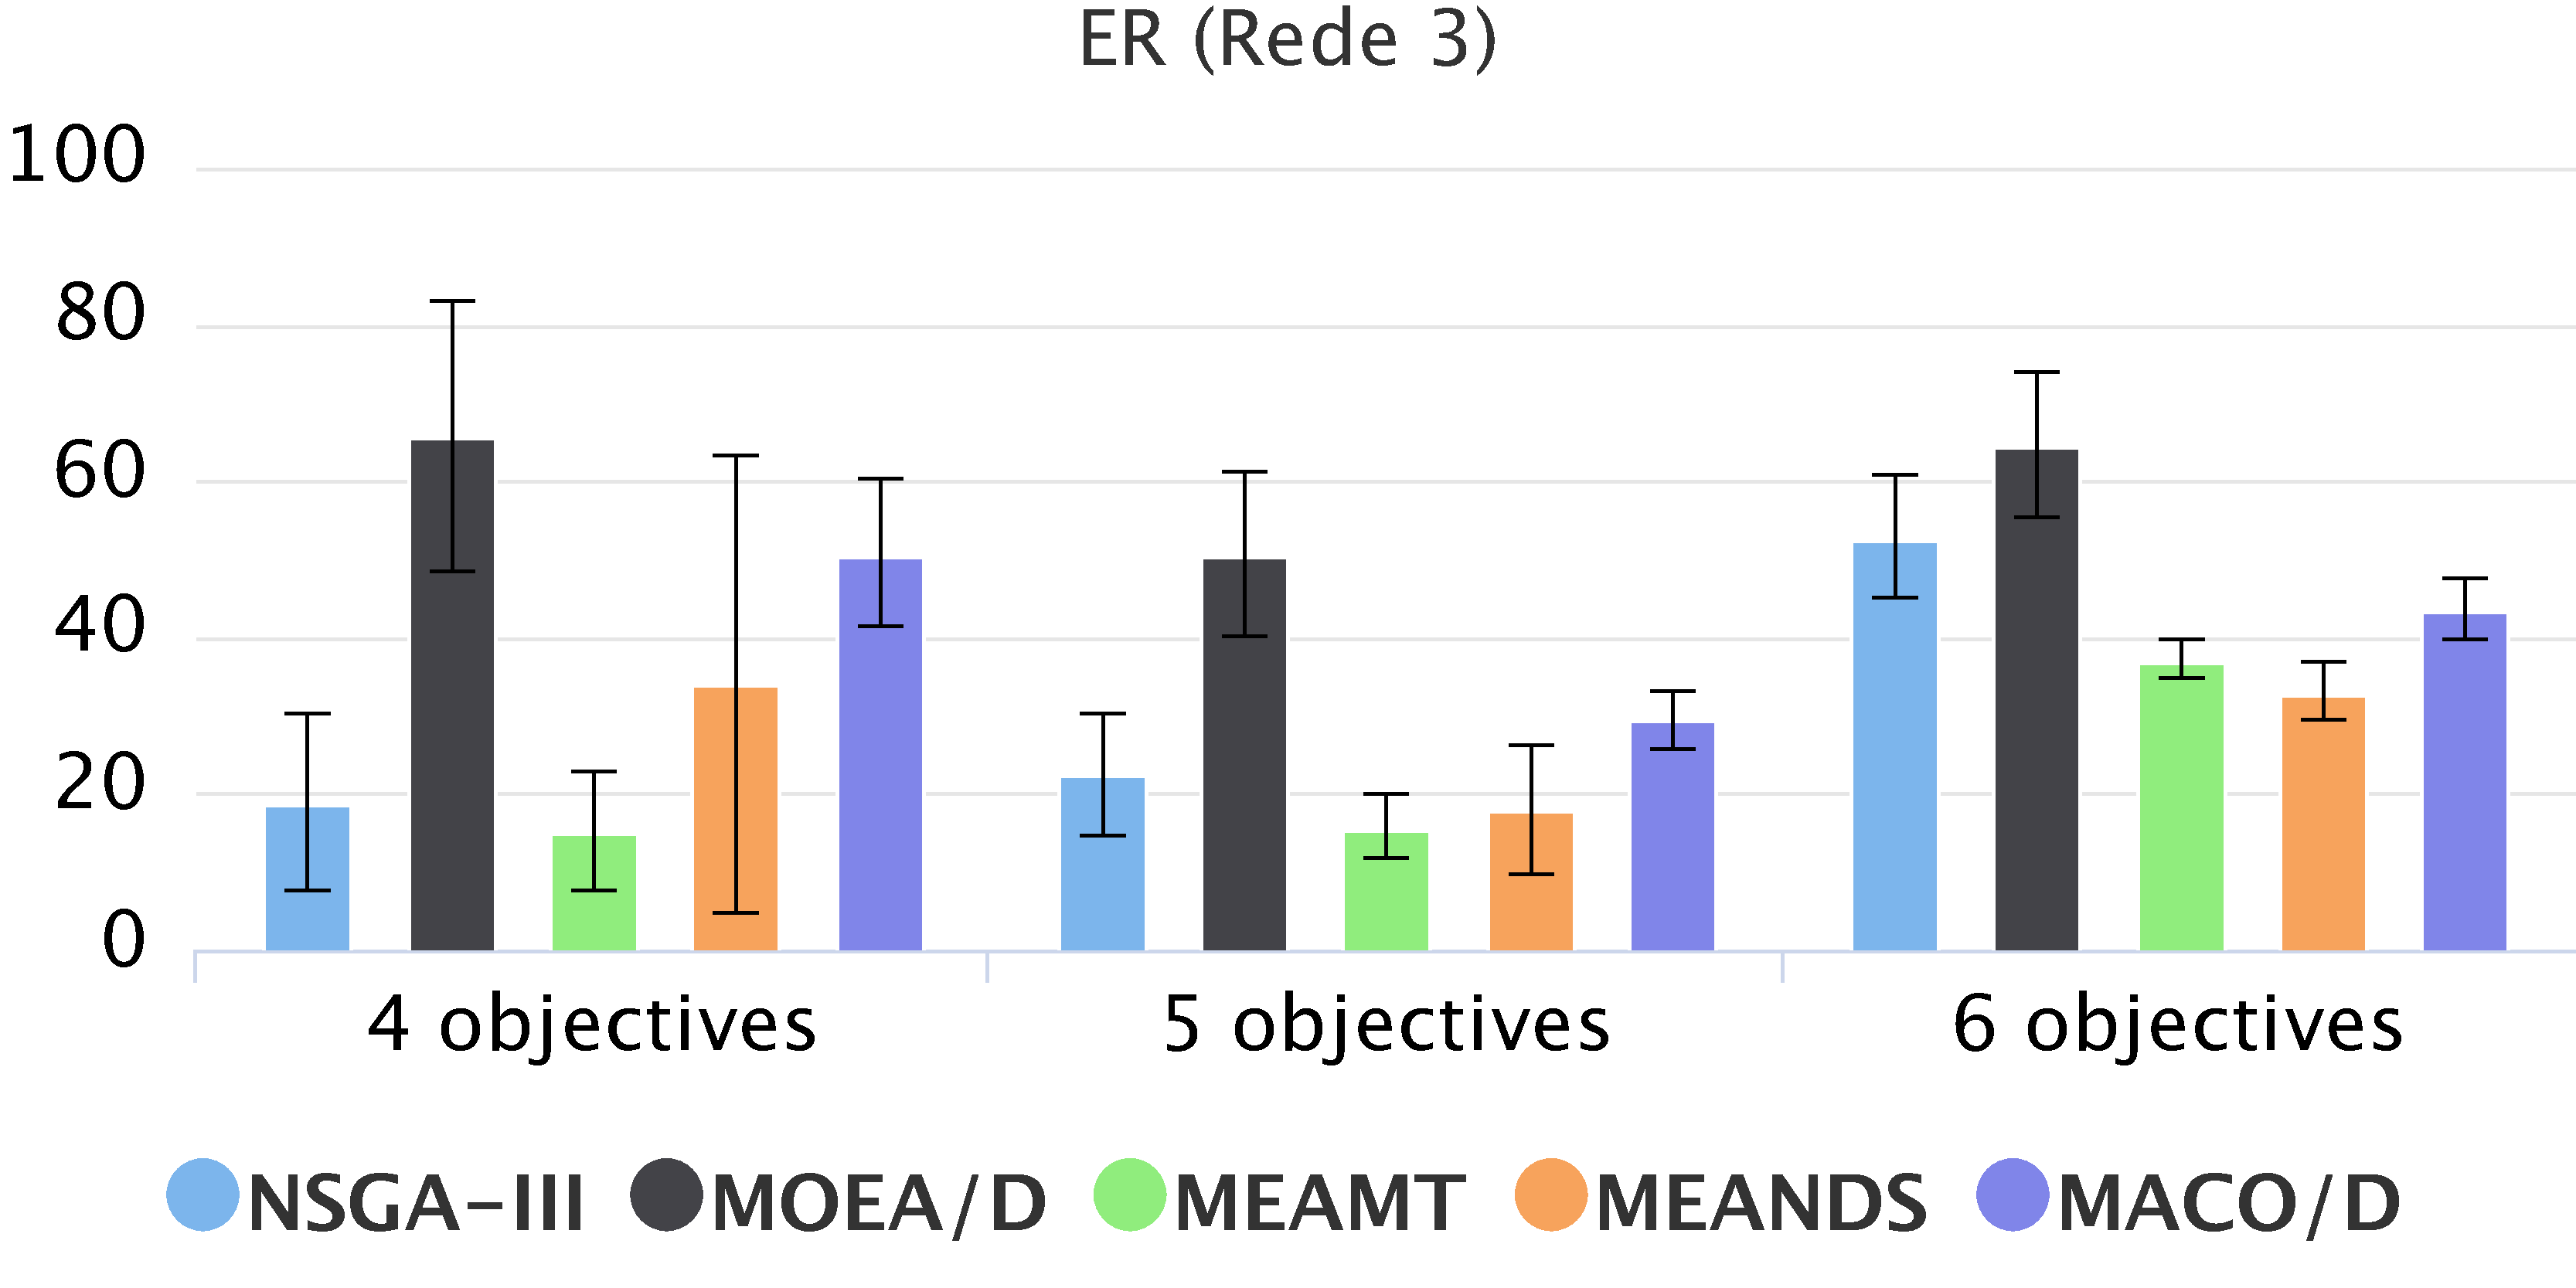
\includegraphics[width=0.5\textwidth]{cap_experimentos/figs/etapa2/er-mrp-r3}
	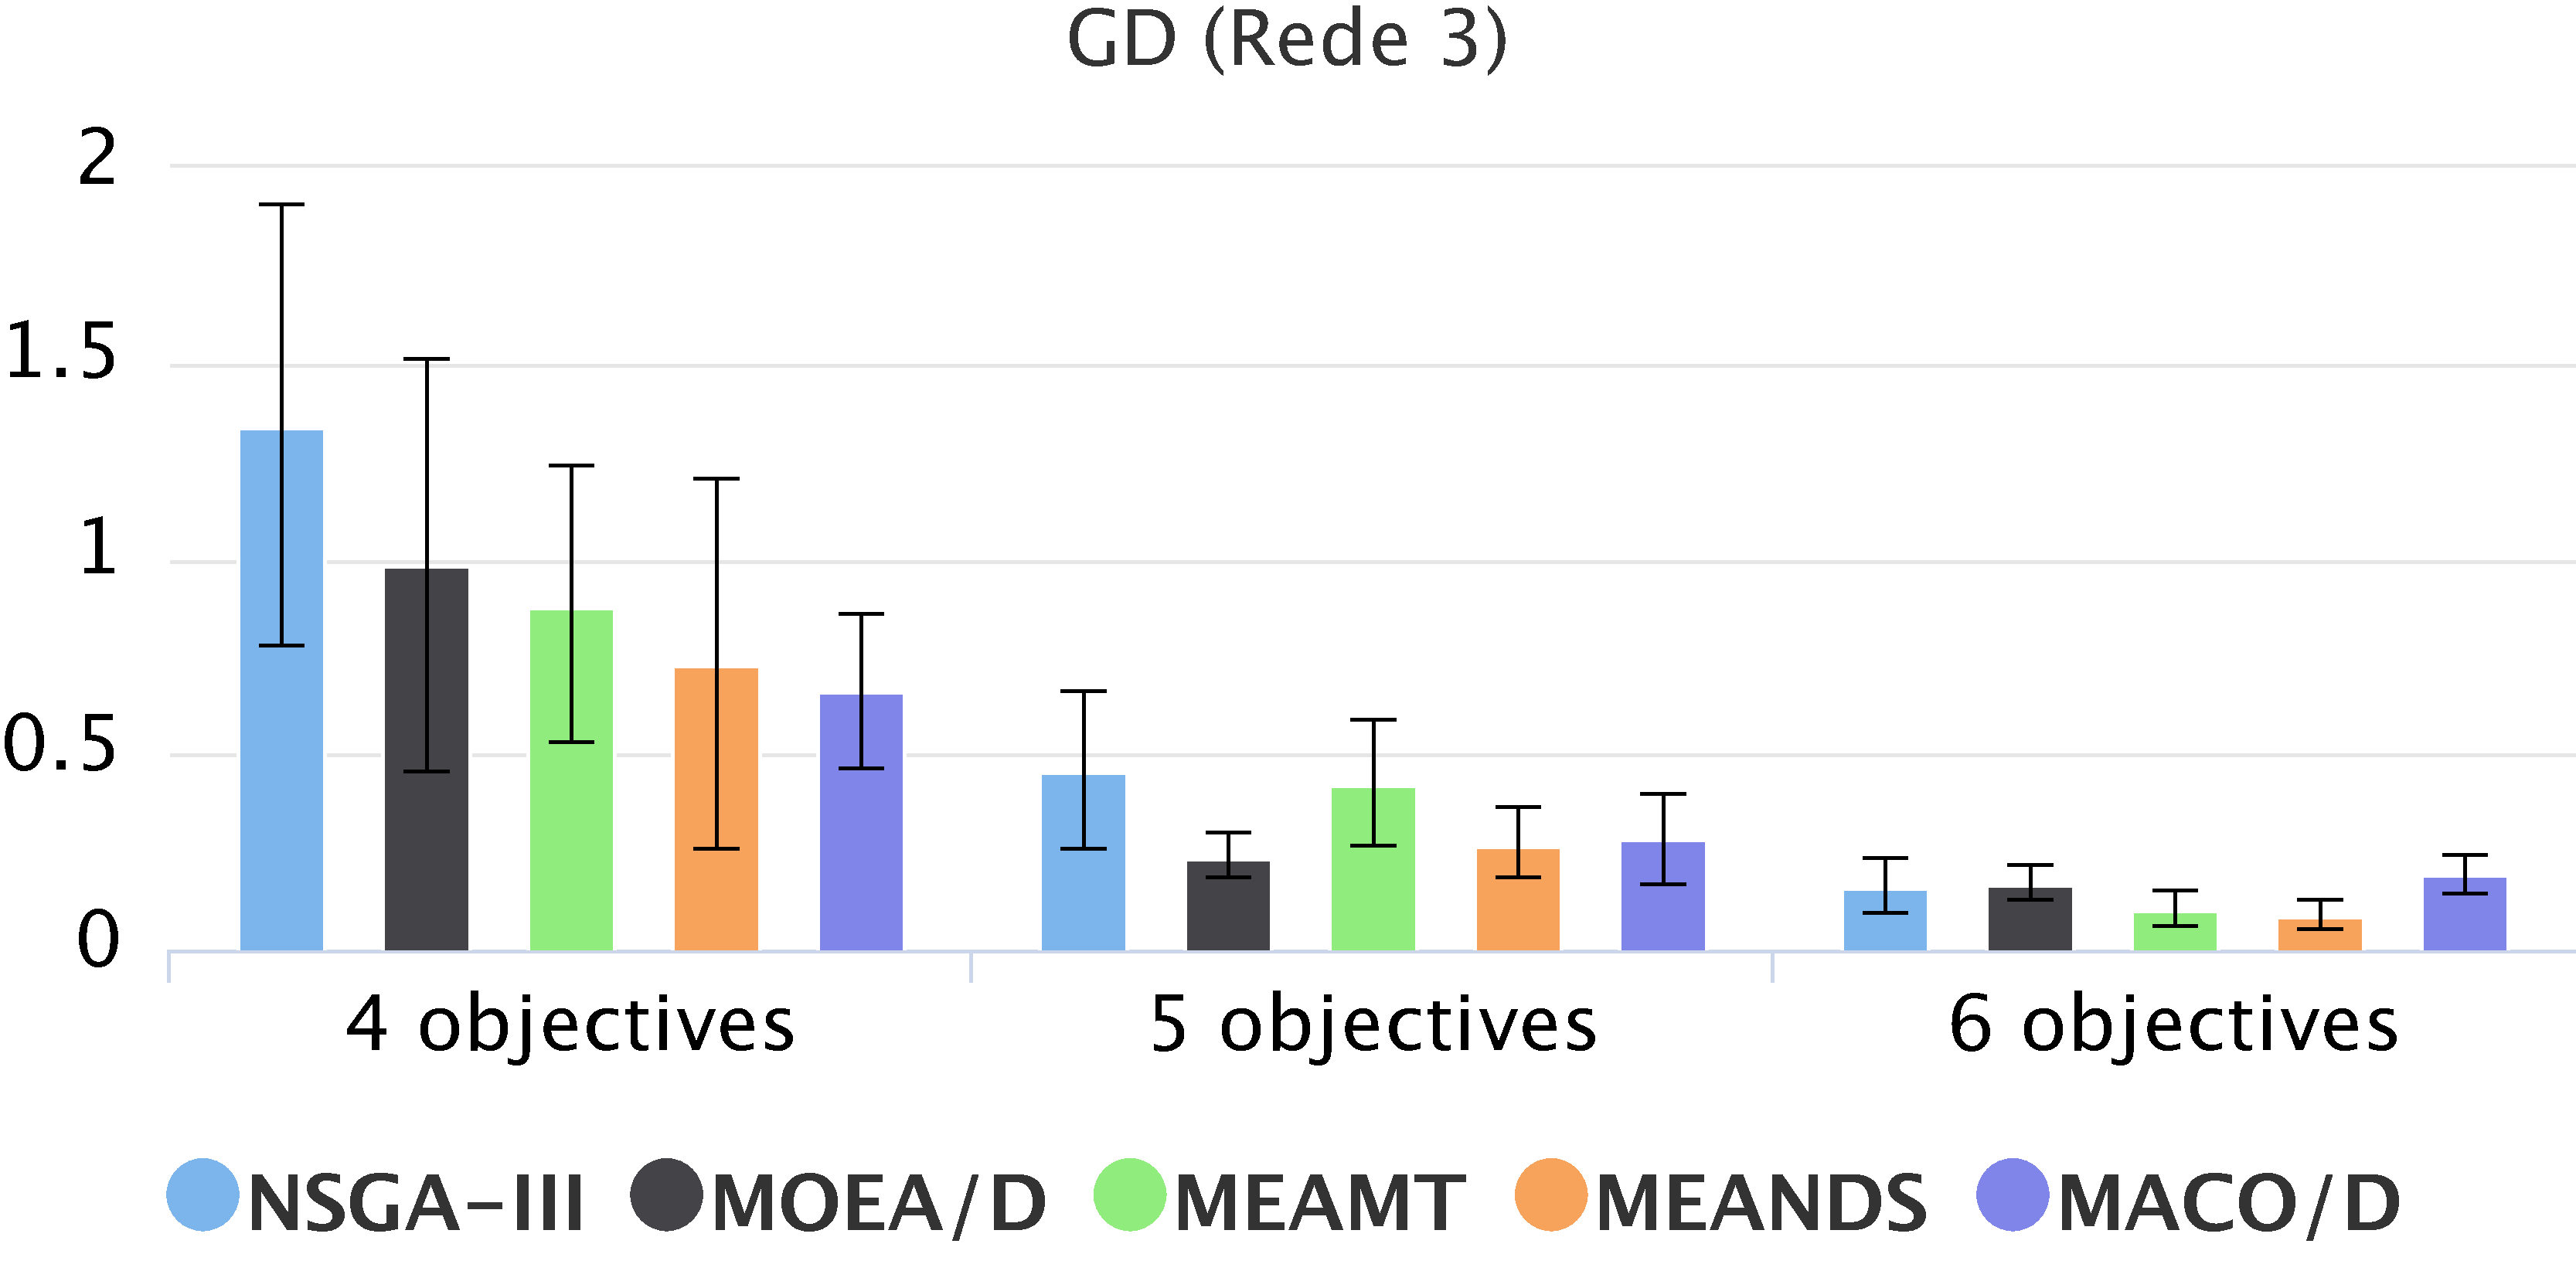
\includegraphics[width=0.5\textwidth]{cap_experimentos/figs/etapa2/gd-mrp-r3}
	\includegraphics[width=0.5\textwidth]{cap_experimentos/figs/etapa2/ps-mrp-r3}
	\includegraphics[width=0.5\textwidth]{cap_experimentos/figs/etapa2/time-mrp-r3}
\end{figure*}

Análise do PRM-R3

\begin{figure*}[!htbp]
	\caption{Etapa 2: resultados agrupados para o PRM nas redes $R_1$, $R_2$ e $R_3$}
	\label{fig_exp2_mrp_todos}
	\includegraphics[width=0.5\textwidth]{cap_experimentos/figs/etapa2/er-mrp-todos}
	\includegraphics[width=0.5\textwidth]{cap_experimentos/figs/etapa2/gd-mrp-todos}
	\includegraphics[width=0.5\textwidth]{cap_experimentos/figs/etapa2/ps-mrp-todos}
	\includegraphics[width=0.5\textwidth]{cap_experimentos/figs/etapa2/time-mrp-todos}
\end{figure*}

Análise geral do PRM

Análise geral dos resultados comparando os dois problemas.

\section{Etapa 3: Análise com hipervolume}

A fim de testar propriamente o comportamento dos algoritmos em espaços de busca mais complexos que os utilizados nos experimentos das etapas 1 e 2, lançou-se mão de três novas redes e instâncias do problema da mochila com 100 e 200 itens. Como não é possível extrair Paretos estáveis para as redes $R_4$, $R_5$ e $R_6$, nem para os problemas da mochila com 50, 100 e 200 itens, não é interessante basear-se em métricas dependentes de tais Paretos para se tirar conclusões. Por isso, nesta etapa, testa-se unicamente a métrica hipervolume, independente do Pareto.

O hipervolume foi utilizado pela primeira vez em [] e desde então, junto a \textit{inverse generational distance} $(IDG)$ [], é a métrica mais utilizada na literatura para se avaliar algoritmos many-objectives. O hipervolume, como explicado no início deste capítulo, calcula o volume da figura geométrica formada pelas distâncias das soluções a um ponto de referência pré-definido. Os pontos de referência utilizados em cada cenário são apresentados na tabela [].

Tabela de pontos de referência.

Nesta etapa testou-se os algoritmos NSGA-III, SPEA2-SDE, MOEA/D, AEMMT, AEMMD, MOACS e MACO/D. Foram 3 formulações de objetivo para cada problema (4, 5 e 6 objetivos) e 3 instâncias, totalizando 18 cenários de teste. Foram realizadas 10 execuções para cada algoritmo em cada cenário e os resultados foram calculados através das médias dos hivervolumes de cada execução.

Falar sobre figuras.
Exibir figuras.
Discutir resultados.